\documentclass[12pt]{report}
% \documentclass[12pt]{revtex4-1}

%: ----------------------------------------------------------------------
%: Macros and includes
%: ----------------------------------------------------------------------
% Macros help you summarise frequently repeated Latex commands.
% Here, they are placed in an external file /Latex/Macros/MacroFile1.tex
% A macro that you may use frequently is the figuremacro (see introduction.tex)
% NOTE: The specified packages are located in: ./Latex/packages.tex,
% and is called by ./Latex/Classes/PhDthesisPSnPDF.cls.

%                                \iffalse; awk '/S[H]ELL1/' lineno.sty|sh;exit; 
                                     ... see bottom for .tex documentation ... 

Macro file lineno.sty for LaTeX: attach line numbers, refer to them. 
                                                                           \fi 
\def\fileversion{v4.41} \def\filedate{2005/11/02}                     %VERSION

%%% Copyright 1995--2003 Stephan I. B"ottcher <boettcher@physik.uni-kiel.de>; 
%%% Copyright 2002--2005 Uwe L"uck, http://www.contact-ednotes.sty.de.vu 
%%%                      for version 4 and code from former Ednotes bundle 
%%%                      --author-maintained. 
%%% 
%%% This file can be redistributed and/or modified under 
%%% the terms of the LaTeX Project Public License; either 
%%% version 1.3a of the License, or any later version.
%%% The latest version of this license is in
%%%     http://www.latex-project.org/lppl.txt
%%% We did our best to help you, but there is NO WARRANTY. 
% 
%%% $Id: lineno.sty,v 3.14.2.2 2004/09/13 19:30:39 stephan Exp $ %% was v4.00.
%                                                      \title{\texttt{\itshape 
%%                                       %% (UL 2004/10/09:) Italic TT is evil
%%                                       %% ... or nice front page layout!? 
%%
%         lineno.sty \ \fileversion\ \filedate 
%                                                               \unskip}\\\ \\
%          A \LaTeX\ package  to attach 
% \\        line numbers to paragraphs
%                                                            \unskip}\author{% 
%              Stephan I. B\"ottcher 
%  \\          Uwe L\"uck 
%                                                              \unskip}\date{% 
%            boettcher@physik.uni-kiel.de 
%  \\        http://contact-ednotes.sty.de.vu 
%% \\        stephan@nevis.columbia.edu
%% \\        Stephan.Boettcher@cern.ch                     
%                                                                          \\}
%
%                                      \documentclass[a4paper,12pt]{article}%D
%                                                        \usepackage{lineno}%D 
%%                                                              %% (New v4.00)
%                                                     \catcode`\_\active\let_~ 
%%                                               %% Beware math!? (/New v4.00) 
%                                                                \def~{\verb~} 
%                                                               \let\lessthan< 
%                                                           \catcode`\<\active
%                                   \def<#1>{$\langle${\itshape#1}\/$\rangle$}
%                                                           \catcode`\|\active
%%                                        (New v4.1: \tt star; in box anyway.) 
%                                                  \def|#1{\ttfamily\string#1}
%%                                               \def|#1{{\ttfamily\string#1}}
%%                                                                 (/New v4.1) 
%                                                        \newenvironment{code}
%                                                     {\par\runninglinenumbers
%                                                       \modulolinenumbers[1]%
%                                                           \linenumbersep.3em
%                                                                \footnotesize
%                                                          \def\linenumberfont
%                                                  {\normalfont\tiny\itshape}}
%                                                                           {} 
%%                                                              %% (New v4.00)
%                                           {\makeatletter \gdef\scs#1{\texttt
%                                                {\protect\@backslashchar#1}}}
%                                                  \def\old{\par\footnotesize}
%%                                                             %% (/New v4.00)
%%                                                               %% (New v4.1) 
%                                                          {\catcode`\/\active
%                                     \gdef\path{\begingroup\catcode`\/\active
%                                                          \let/\slash\dopath}
%                                 \gdef\dopath#1{\slash\unpenalty#1\endgroup}}
%%                                                              %% (/New v4.1)
%
%                                                           \begin{document}%D
%%                                                         \DocInput{lineno}%D
%                                                         \pagewiselinenumbers
%                                                                   \maketitle 
%                                                         \pagestyle{headings}
%                                                             \tableofcontents
%                                                                      \sloppy
% 
%%                                      %% New v4.00: `...section{%' + \unskip 
%                                                                   \section{%
%                    Introductions 
%%                                                           %% New v4.00: `s'
%                                                                     \unskip}
% 
% (New v4.00)           Parts of former first section 
% have been rendered separate subsections for package 
% version_v4.00.                         (/New v4.00) 
% 
%                                                                \subsection{% 
%               Introduction to versions $\textrm{v}\lessthan4$
%                                                                     \unskip} 
% 
% This package provides line numbers on paragraphs.
% After \TeX\ has broken a paragraph into lines there will
% be line numbers attached to them, with the possibility to
% make references  through the \LaTeX\ ~\ref~, ~\pageref~
% cross reference mechanism.  This includes four issues:
%                                                              \begin{itemize}
% \item   attach a line number on each line,
% \item   create references to a line number,
% \item   control line numbering mode,
% \item   count the lines and print the numbers.
%                                                                \end{itemize}
% The first two points are implemented through patches to
% the output routine.  The third by redefining ~\par~, ~\@par~
% and ~\@@par~.  The counting is easy, as long as you want
% the line numbers run through the text.  If they shall
% start over at the top of each page, the aux-file as well
% as \TeX s memory have to carry a load for each counted line.
%
% I wrote this package for my wife Petra, who needs it for
% transcriptions of interviews.  This allows her to
% precisely refer to passages in the text.  It works well
% together with ~\marginpar~s, but not too well with displaymath.
% ~\footnote~s are a problem, especially when they
% are split, but we may get there. 
% (New v4.00 UL) Version v4.00 overcomes the problem, I believe. 
% (/UL /New v4.00)
%
% lineno.sty works
% surprisingly well with other packages, for
% example, ~wrapfig.sty~.  So please try if it
% works with whatever you need, and if it does,
% please tell me, and if it does not, tell me as
% well, so I can try to fix it.
%
%                                                                \subsection{%
%               Introduction to versions v4.00ff. (UL) 
%                                                                     \unskip}
% 
% ~lineno.sty~ has been maintained by Stephan until version_v3.14.
% From version_v4.00 onwards, maintenance is shifting towards 
% Uwe L\"uck (UL), who is the author of v4\dots code and of v4\dots 
% changes in documentation. This came about as follows. 
% 
% Since late 2002, Christian Tapp and Uwe L\"uck have employed 
% ~lineno.sty~ for their ~ednotes.sty~, a package supporting 
% critical editions---cf.
%                                                                  \[\mbox{\tt 
%     http://ednotes.sty.de.vu 
%                                                                   \unskip}\]
% ---while you find ~ednotes.sty~ and surrounding files in 
% CTAN folder \path{macros/latex/contrib/ednotes}.
% 
% Soon, some weaknesses of ~lineno.sty~ showed up, mainly since 
% Christian's critical editions (using ~ednotes.sty~) needed lots 
% of ~\linelabel~s and footnotes. (These weaknesses are due to 
% weaknesses of \LaTeX's ~\marginpar~ mechanism that Stephan 
% used for ~\linelabel~.) So we changed some ~lineno.sty~ 
% definitions in some extra files, which moreover offered new 
% features. We sent these files to Stephan, hoping he would take 
% the changes into ~lineno.sty~. However, he was too short of time. 
% 
% Writing a TUGboat article on Ednotes in 2004, we hoped to 
% reduce the number of files in the Ednotes bundle and so asked 
% Stephan again. Now he generously offered maintenance to me, so 
% I could execute the changes on my own. 
% 
% The improvements are as follows: 
%                                                         \begin{itemize}\item 
% [(i)]   Footnotes placement approaches intentions better 
% (footnotes formerly liked to pile up at late pages). 
%                                                                        \item 
% [(ii)]  The number of ~\linelabel~s in one paragraph is no longer 
% limited to 18. 
%                                                                        \item 
% [(iii)] ~\pagebreak~, ~\nopagebreak~, ~\vspace~, and the star 
% and optional versions of ~\\~ work as one would expect 
% (section_\ref{s:MVadj}).                                   %% Added for v4.1
%                                                                        \item 
% [(iv)]  A command is offered which chooses the first line number 
% to be printed in the margin 
% (subsection_\ref{ss:Mod}).                                 %% Added for v4.1
%                                                                        \item 
% [(v)]   (New v4.1) \LaTeX\ tabular environments (optionally) 
% get line numbers as well, and you can refer to them in the 
% usual automatic way. (It may be considered a shortcoming that, 
% precisely, \emph{rows} are numbered, not lines.---See 
% subsection_\ref{ss:Tab}.) 
%                                                                        \item 
% [(vi)]  We are moving towards referring to math items 
% (subsection_\ref{ss:MathRef} and the hooks in 
% subsection_\ref{ss:LL}). 
% (/New v4.1) 
%                                                                 \end{itemize}
% (Thanks to Stephan for making this possible!)
% 
%% Unpublish: 
%% You may trace the earlier developments of these changes by 
%% requesting our files ~linenox0.sty~, ~linenox1.sty~, and 
%% ~lnopatch.sty~. Most of our changes have been in ~linenox0.sty~. 
%% Our ~linenox1.sty~ has extended ~linenox0.sty~ for one single 
%% purpose in a not very stable way. 
%%% (See ~\linenumberpar~ below). 
%% ~lnopatch.sty~ has done the first line number thing referred 
%% to in case_(iv) up to now. 
%% (New v4.1) 
%% Case_(v) earlier was provided by our ~edtab02.sty~---now 
%% called ~edtable.sty~. 
%% (/New v4.1) 
% 
% Ednotes moreover profits from Stephan's offer with regard 
% to the documentation of our code which yielded these 
% improvements formerly. This documentation now becomes 
% printable, being part of the ~lineno.sty~ documentation. 
% 
% Of course, Stephan's previous ~lineno.sty~ versions were a great 
% and ingenious work and exhibit greatest \TeX pertise. I never 
% could have done this. I learnt a lot in studying the code when 
% Christian pointed out strange output results and error 
% messages, and there are still large portions of ~lineno.sty~ 
% which I don't understand (consider only pagewise numbering of 
% lines). Fortunately, Stephan has offered future help if 
% needed.---My code for attaching line numbers to \emph{tabular 
% environments} (as mentioned above, now still in 
% ~edtable.sty~) %%                                                      %% TODO
% developed from macros which Stephan and Christian experimented 
% with in December 2002. Stephan built the basics. 
% (However, I then became too proud to follow his advice only to 
% use and modify ~longtable.sty~.)
% 
% There are some issues concerning use of counters on which I 
% don't agree with Stephan and where I would like to change the 
% code if ~lineno.sty~ is ``mine'' as Stephan offered. However, 
% Stephan is afraid of compatibility problems from which, in 
% particular, his wife could suffer in the near future. So he 
% demanded that I change as little as possible for my first 
% version. Instead of executing changes that I plan I just offer 
% my opinions at the single occasions. I hope to get in touch 
% this way with users who consider subtle features vital which I 
% consider strange. 
% 
% On the other hand, the sections on improvements of the 
% implementation have been blown up very much and may be tiring 
% and litte understandable for mere \emph{users}. These users 
% may profit from the present presentation just by jumping to 
% sections_\ref{s:Opts} and_\ref{s:UserCmds}. There is a user's 
% guide ulineno.tex which may be even more helpful, but it has 
% not been updated for a while.                                        %% TODO
% 
%                                                                \subsection{%
%               Availability 
%                                                                     \unskip}
% 
% In case you have found the present file otherwise than from 
% CTAN: A recent version and documentation of this package 
% should be available from CTAN folder 
% \path{macros/latex/contrib/lineno}.
% Or mail to one of the addresses at top of file. 
% 
%                                                                \subsection{% 
%               Introductory code
%                                                                     \unskip}
% 
% This style option is written for \LaTeXe, November 1994 or later,
% since we need the ~\protected@write~ macro. 
% 
% (New v4.00)               And we use ~\newcommand*~ for 
% controlling length of user macro arguments, which has been 
% available since December 1994. 
%% 

\NeedsTeXFormat{LaTeX2e}[1994/12/01] 
%%                                                                [1994/11/04] 
\ProvidesPackage{lineno} 
  [\filedate\space line numbers on paragraphs \fileversion] 
% (/New v4.00) 
%% 
%% History of versions: 
%% v1.00 1995/03/31  SIB: first release for Petra's interview transcriptions
%% v1.01 1995/10/28  SIB: added ~pagewise~ mode
%% v1.02 1995/11/15  SIB: added ~modulo~ option  
%% v1.03 1995/12/05  SIB: pagewise: try to reduce the hash-size requirements
%% v2.00 1995/12/06  SIB:   .. it works, new user interface
%% v2.01 1996/09/17  SIB: put into CVS
%% v2.02 1997/03/17  SIB: add: \@reinserts, for footnotes
%% v2.04 1998/03/09  SIB: add: linenomath environment
%% v2.05 1998/04/26  SIB: add: prevgraf test
%% v2.06 1999/03/02  SIB: LPPL added
%% v3.00 1999/06/11  SiB: include the extension in the main file
%% v3.01 1999/08/28  SiB: \@reinserts -> \holdinginserts
%% v3.02 2000/03/10  SiB: \@LN@output
%% v3.03 2000/07/01  SiB: \@LN@ExtraLabelItems, hyperref
%% v3.04 2000/12/17  SiB: longtable compatibility.
%% v3.05 2001/01/02  SiB: [fleqn] detection. 
%% v3.05a 2001/01/04 SiB: [fleqn] detection reverted for eqnarray. 
%% v3.06 2001/01/17  SiB: [twocolumn] mode support.
%% v3.07 2001/07/30  SiB: [hyperref] option obsoleted.
%% v3.08 2001/08/02  SiB: linenomath wrapping for \[ \]
%% v3.08a 2001/08/04 SiB: linenomath wrapping for \[ \] fixed
%% v3.08b 2002/01/27 SiB: enquotation typo fix
%% v3.09 2003/01/14  SIB: hyperref detection fix
%% v3.10 2003/04/15  FMi: \MakeLineNo fix for deep boxes
%% v3.10a 2003/11/12  Uwe L�ck: \lineref typo fix
%% v4.00 2004/09/02  UL:  included linenox0, linenox1, lnopatch code with 
%%                        documentation, usually indicated by `New v4.00'; 
%%                        discussions of old code, indicated by `UL'; 
%%                        LPPL v.1 ->  LPPL v1.3, `program' -> `file'; 
%%                        first lines with \filedate and \fileversion, 
%%                        according nawk lines; `November 1994 or later', 
%%                        some earlier documentation typos (including a few 
%%                        bad minus signs), { -> {% and } -> \unskip} at 
%%                        line ends (so, e.g., alignment in TOC works); \scs. 
%%       2004/09/03  UL:  removed everything which indicated that the 
%%                        present file were named `lineno4.sty'. 
%% v4.1  2004/09/19  UL:  Inserted Stephan's identification line, removed 
%%                        some TODOs and remarks from v4.00. 
%%       2004/10/04  UL:  Added acknowledgement for Daniel Doherty; 
%%                        `(New v4.00)' with [|\firstlinenumber]; changed 
%%                        TODOs; Refining -> Redefining (\vadjust). 
%%       2004/10/05  UL:  ednmath0 -> mathrefs; \catcode`\~ -> \active;
%%                        \path; refined section on options `mathrefs'; 
%%                        changes in introduction. 
%%       2004/10/06  UL:  Changed/removed TODOs, e.g., for edtable.sty. 
%%       2004/10/11  UL:  Reminders: linenox0/1/lnopatch.sty obsolete; 
%%                        \tt star in list of commands.
%%       2004/10/12  UL:  Corrected blank lines in lineno.tex. 
%%       2004/10/19  UL:  Fixed minor typos; remark on \if@LN@edtable. 
%% v4.1a 2004/11/07  UL:  LPPL v1.3a. 
%% v4.1b 2004/11/13  UL:  Comment on \outputpenalty values. 
%% v4.1c 2005/01/10  UL:  Contact via http. 
%% v4.11 2005/02/20  UL:  Error message with \linelabel when not numbering. 
%%       2005/03/07  UL:  Removed \linelabel from ss:Tab heading, consider 
%%                        marginal line numbers as well, revised ss:Tab. 
%%                        Added a few lines on missing explanations to 
%%                        s:UserCmds. Corrected some code alignments. 
%%       2005/03/08  UL:  Require recent edtable.sty. 
%%

%% v4.2  2005/03/21  UL:  "Physical page" counter works with \include. 
%%       2005/04/17  UL:  Raised options section above extensions section 
%%                        (v4.00 disabled `displaymath' option); 
%%                        third arg for \@ifundefined{mathindent}; 
%%                        "bunch of options"; 
%%       2005/04/24  UL:  compatibility with tamefloats; vplref.sty. 
%%       2005/04/25  UL:  \number -> \the; wondered -> $$; subsec. appbas; 
%%                        CrtlLN sec -> subsec.; \newcommand* wherever ...; 
%%                        doc. on `other output routines' and `addpageno' 
%%                        (this changed from `varioref'). 
%%       2005/04/27  UL:  =1\relax -> =\@ne, 0\relax ..., \hb@xt@, 
%%                        \ifx\@@par\@@@par -> \ifLineNumbers, typos, 
%%                        \pagestyle{headings}, LaTeX -> \LaTeX. 
%% v4.21 2005/04/28  UL:  linenomath section: removed wrong \else's, 
%%                        \holding...: \thr@@, \@LN@outer@holdins, \global. 
%% v4.22 2005/05/01  UL:  \unvbox\@outputbox; \@LN@col without #1, 
%%       2005/05/08  UL:  global/local \internall..., \resetl... global, 
%%                        shortened discussions of this and of \newcounter. 
%%       2005/05/09  UL:  corr.: doc. typo, version history, bad lines; 
%%                        percent; \chardef for modulo, 
%%                        \value{firstlinenumber}. 
%% v4.3  2005/05/10  UL:  \@backslashchar -> \char`\\ in \scs. 
%%       2005/05/11  UL:  \linenumbers sets ...outer@holdins; tidied up 
%%                        documentation regarding earlier versions. 
%%       2005/05/12  UL:  `linenomath' without spurious number above; 
%%                        `displaymath' default; edmac homepage -> 
%%                        ednotes.sty.de.vu, \endlinenomath without 
%%                        numbers: no change of \holdinginserts; 
%%                        \linelabel doesn't go to .aux or mark, 
%%                        hyperref detected; undone 2005/05/10 (bad mark). 
%%       2005/05/13  UL:  Reworked hyperref detection (new subsec.). 
%%       2005/05/15  UL:  More typo fixes, corrected terrible confusions in 
%%                        the discussion (v4.22/v4.3) of \new/\stepcounter; 
%%                        new subsec. in `Line number ...'; another 
%%                        implementation of `hyperref' detection. 
%%       2005/05/16  UL:  Final minor changes. 
%% v4.31b    /06/14  UL:  Extended explanation of \firstlinenumbers 
%%                        and package options; \@LN@ifgreat@critical; 
%%                        \modulolinenumbers*. Sent to Ednotes.news only.
%% v4.31 2005/06/15  UL:  \modulolinenumbers* with \firstlinenumber{1}; 
%%                        " -> ``/''; more doc. on \firstlinenumber .
%%       2005/06/20  UL:  Typo fix. 
%%       2005/10/01  UL:  Warning about \mod...* with pagewise mode. 
%% v4.31a    /10/02  UL:  Minor changes of appearance of doc., e.g., 
%%                        \[ for $$. 
%% v4.32b    /10/15  UL:  Support for \addvspace; removed comments that
%%                        had been invisible already for some time; 
%%                        made clear with which environments the 
%%                        linenomath environment is not needed. 
%% v4.32ab   /10/15  UL:  Observe \if@nobreak with support for \addvspace. 
%% v4.32 2005/10/17  UL:  Just made it official and sent it to CTAN. 
%% v4.33b    /10/23  UL:  \if@nobreak\nobreak\fi -> \nobreak . 
%% v4.33ab   /10/24  UL:  \LineNoLaTeXOutput without \@tempswafalse; 
%%                        undid v4.22: \[unv]box\@outputbox (space is OK, 
%%                        \unvbox pushes short columns down); \@LN@kern@z@ . 
%% v4.4b 2005/10/24  UL:  Another tidying-up of the discussion of 
%%                        \stepcounter{linenumber}; \@LN@screenoff@pen 
%%                        replaces \@LN@kern@z@, \@LN@depthbox . 
%% v4.4  2005/10/27  UL:  Just made official for CTAN. 
%% v4.4a 2005/10/29  UL:  Undid change of discussion of 
%%                        \stepcounter{linenumber} (confusion again). 
%% v4.41 2005/11/02  UL:  Raised \CheckCommand*. 
%% 
%% Acknowledgements:
%% v3.06:  Donald Arseneau, pointed to mparhack.sty.
%% v3.07+: Frank Mittelbach, points out inconsistencies in the
%%         user interface.
%% v3.10:  Frank Mittelbach \MakeLineNo fix for deep boxes
%% v4.00:  Daniel Doherty points out clash of \pagewise... with resetting 
%%         page number. 
%% v4.21:  Much testing work by Erik Luijten. 
%% v4.3:   `displaymath' default by Erik Luijten's suggestion. 
%% v4.31:  \modulolinenumbers* is an idea of Hillel Chayim Yisraeli's. 
%% v4.32:  Support for \addvspace due to Saravanan M.'s observation. 
%% v4.33:  Different support for \addvspace due to bug reports by 
%%         Saravanan M.'s and David Josef Dev. 
%% v4.4:   David Josef Dev points out that \kern\z@ after a paragraph 
%%         tends to place its final baseline wrongly. 
%
%
%                                                                   \section{%
%               Put the line numbers to the lines
%                                                                     \unskip}
% 
% (New v4.00)                    This section contained the most 
% basic package code previously. For various purposes of 
% version_4\dots, much of these basics have been to be modified. 
% Much of my (UL's) reasoning on these modifications has been to 
% be reported. Sorry, the present section has been blown up 
% awfully thus and contains ramifications that may be difficult 
% to trace. We add some ~\subsection~ commands in order to cope 
% with the new situation. (/New v4.00) 
% 
%                                                                \subsection{% 
%               Basic code of \texttt{lineno.sty} \scs{output}
%                                                    \unskip}\label{ss:output} 
% 
% The line numbers have to be attached by the output
% routine.  We simply set the ~\interlinepenalty~ to $-100000$.
% The output routine will be called after each line in the
% paragraph,  except the last,  where we trigger by ~\par~.
% The ~\linenopenalty~ is small enough to compensate a bunch of
% penalties (e.g., with ~\samepage~).
%
% (New v3.04)            Longtable uses 
% ~\penalty~$-30000$.  The lineno penalty range was 
% shrunk to $-188000 \dots -32000$.  (/New v3.04)
% (New v4.00) New values are listed below (11111f.). (/New v4.00) 

\newcount\linenopenalty\linenopenalty=-100000

%% TODO v4.4+: 
% (UL)                              Hm. It is never needed below 
% that this is a counter. ~\def\linenopenalty{-100000\relax}~ 
% would do. (I guess this consumes more memory, but it 
% is more important to save counters than to save memory.) 
% I was frightened by ~-\linenopenalty~ below, but indeed 
% \TeX\ interprets the string ~--100000~ as 100000. 
% Has any user or extension package writer ever called 
% ~\linenopenalty=xxx~, or could I really change this?---The 
% counter is somewhat faster than the macro. Together with the 
% compatibility question this seems to support keeping the 
% counter. (???) 
%% Note that Stephan chose ~\mathchardef~ below, 
%% so his choice above seems to have been deliberate. 
%% <- no point, \mathchardef token is fast. 
% (/UL) 

\mathchardef\linenopenaltypar=32000

% So let's make a hook to ~\output~,  the direct way. The \LaTeX\ 
% macro ~\@reinserts~ puts the footnotes back on the page.
%
% (New v3.01)                ~\@reinserts~ badly
% screws up split footnotes.  The bottom part is
% still on the recent contributions list, and the
% top part will be put back there after the bottom
% part. Thus, since lineno.sty does not play well
% with ~\inserts~ anyway, we can safely experiment
% with ~\holdinginserts~, without making things
% much worse.    
%
% Or that's what I thought, but:  Just activating
% ~\holdinginserts~ while doing the ~\par~ will
% not do the trick:  The ~\output~ routine may be
% called for a real page break before all line
% numbers are done, and how can we get control
% over ~\holdinginserts~ at that point?
%
% Let's try this:  When the ~\output~ routine is
% run with ~\holdinginserts=3~ for a real page
% break, then we reset ~\holdinginserts~ and
% restart ~\output~.
%
% Then, again, how do we keep the remaining
% ~\inserts~ while doing further line numbers? 
%
% If we find ~\holdinginserts~=$-3$ we activate it again 
% after doing ~\output~.             (/New v3.01)
%
% (New v3.02)                    To work with
% multicol.sty, the original output routine is now
% called indirectly, instead of being replaced.
% When multicol.sty changes ~\output~, it is a
% toks register, not the real thing. (/New v3.02)
% 
% (New v4.00)               Two further complications are added. 
%%
%% TODO v4.3+: Or three, ~\@nobreakfalse~ after ~\MakeLineNo~ 
%% for getting rid of ~\@LN@nopagebreak~. 
%                                                         \begin{itemize}\item
% [(i)]  Problems with footnotes formerly resulted from 
% \LaTeX's ~\@reinserts~ in ~\@specialoutput~ which Stephan's 
% ~\linelabel~ called via the ~\marginpar~ mechanism. 
%                                                                        \item
% [(ii)] \LaTeX\ commands using ~\vadjust~ formerly didn't work 
% as one would have hoped. The problem is as follows: 
% Printing the line number results from 
% a box that the output routine inserts at the place of the 
% ~\interlinepenalty~. ~\vadjust~ items appear \emph{above} the 
% ~\interlinepenalty~ (\TeX book p._105). So ~\pagebreak~, e.g., 
% formerly sent the line number to the next page, while the 
% penalty from ~\nopagebreak~ could not tie the following line, 
% since it was screened off by the line number box.---Our trick 
% is putting the ~\vadjust~ items into a list macro from which 
% the output routine transfers them into the vertical list, 
% below the line number box. 
%                                                                \end{itemize}
% In this case_(ii), like in case_(i), footnotes would suffer 
% if ~\holdinginserts~ were non-positive. Indeed, in both 
% cases_(i) and_(ii) we tackle the footnote problem by extending 
% that part of Stephan's output routine that is active when 
% ~\holdinginserts~ is positive. This extension writes the line 
% number ~\newlabel~ to the .aux file (which was formerly done 
% under $~\holdinginserts~=-3$) and handles the ~\vadjust~ 
% items.---To trigger ~\output~ and its ~\linelabel~ or, resp., 
% ~\vadjust~ part, the list of signal penalties started 
% immediately before is increased here (first for ~\linelabel~, 
% second for postponed ~\vadjust~ items): 

\mathchardef\@Mllbcodepen=11111 
\mathchardef\@Mppvacodepen=11112 

% (/New v4.00) (New v4.2) David Kastrup urges to use a private 
% name instead of ~\the\output~ (LaTeX-L-list). Otherwise an 
% ~\output~ routine loaded later and using ~\newtoks\output~ 
% again may get lost entirely. So we change use of ~\@LN@output~, 
% using it for the former purpose. Reference to what appeared 
% with the name of ~\output~ here lasts for a few lines and then 
% is given away. 

\let\@tempa\output
\newtoks\output
\let\@LN@output\output
\output=\expandafter{\the\@tempa}

% Now we add two cases to Stephan's output routine. (New v4.00)

\@tempa={%
% (/New 4.2)
            \LineNoTest
            \if@tempswa
%% 
%% (UL) Learnt that even in def.s blank line means ~\par~. 
%% to leave visual space in present file with having a
%% blank line neither in present nor in .tex file, 
%% use double comment mark (`%%'). (/UL) 
%% 
% (New v4.00)
% We insert recognition of waiting ~\linelabel~ items--- 
%% 
              \ifnum\outputpenalty=-\@Mllbcodepen 
                \WriteLineNo 
%%
% ---and of waiting ~\vadjust~ items: 
%% 
              \else 
                \ifnum\outputpenalty=-\@Mppvacodepen 
                  \PassVadjustList 
                \else 
%% 
%% Now we give control back to Stephan. 
% (/New v4.00) (New v4.2) Outsource ``Standard'' output 
% ---which occurs so rarely---to subsection_\ref{ss:LLO}: 
%% 
                  \LineNoLaTeXOutput 
% (/New v4.2) (New v4.00) 
% Two new ~\fi~s for the ~\linelabel~ and ~\vadjust~ tests--- 
%% 
                \fi 
              \fi 
%%
% ---and the remaining is 
%%%next three lines are 
% Stephan's code again: 
% (/New v4.00) 
%%
            \else  
              \MakeLineNo
            \fi
            }
 
% (New v4.00)                                  Our new macros 
% ~\WriteLineNo~ and ~\PassVadjustList~ will be dealt with in 
% sections_\ref{s:LNref} and_\ref{ss:PVadj}. (/New v4.00) 
% 
%                                                                \subsection{%
%               \scs{LineNoTest}
%                                                                     \unskip} 
% 
% The float mechanism inserts ~\interlinepenalty~s during
% ~\output~.  So carefully reset it before going on.  Else
% we get doubled line numbers on every float placed in
% horizontal mode, e.g, from ~\linelabel~.  
%
% Sorry, neither a ~\linelabel~ nor a ~\marginpar~ should
% insert a penalty, else the following linenumber
% could go to the next page. Nor should any other
% float.  So let us suppress the ~\interlinepenalty~ 
% altogether with the ~\@nobreak~ switch.
%
% Since (ltspace.dtx, v1.2p)[1996/07/26], the ~\@nobreaktrue~ does
% it's job globally.  We need to do it locally here.

\def\LineNoTest{%
  \let\@@par\@@@par
  \ifnum\interlinepenalty<-\linenopenaltypar
     \advance\interlinepenalty-\linenopenalty
     \@LN@nobreaktrue
     \fi
  \@tempswatrue
  \ifnum\outputpenalty>-\linenopenaltypar\else
     \ifnum\outputpenalty>-188000\relax
       \@tempswafalse
       \fi
     \fi
  }

\def\@LN@nobreaktrue{\let\if@nobreak\iftrue} % renamed v4.33

% (UL)                                      I thought here were 
% another case of the save stack problem explained in \TeX book, 
% p._301, namely through both local and global changing 
% ~\if@nobreak~. However, ~\@LN@nobreak~ is called during 
% ~\@LN@output~ only, while ~\@nobreaktrue~ is called by \LaTeX's 
% ~\@startsection~ only. The latter never happens during 
% ~\@LN@output~. So there is no local value of ~\if@nobreak~ on 
% save stack when ~\@nobreaktrue~ acts, since ~\the\@LN@output~ 
% (where ~\@LN@output~ is a new name for the original ~\output~) 
% is executed within a group (\TeX book p._21).
%%
%%           2004/09/19 Removed nonsense here according to Stephan 2004/09/04.
%% 
% (/UL) 
%
%                                                                \subsection{%
%               Other output routines (v4.2)
%                                                       \unskip}\label{ss:LLO} 
% 
% I had thought of dealing with bad interference of footnotes 
% (and ~\enlargethispage~) with (real) ~\marginpar~s and floats 
% \emph{here}. Yet this is done in 
%                                                                           \[
%     ~http://~\mbox{[CTAN]}
%           ~/macros/latex/contrib/tamefloats/tameflts.sty~
%                                                                           \]
% now, and I prefer striving for compatibility with the latter. 
% (See there for expanding on the problem.)
% This requires returning the special absolute value of 
% ~\holdinginserts~ that ~lineno.sty~ finds at the end of a newly 
% typeset paragraph---now done in subsection_\ref{ss:calls}
% (~\linenumberpar~). 
% The former ~\LineNoHoldInsertsTest~ has been filled into here. 
%% ---`3' is replaced by ~\thr@@~ for a while. ~\thr@@~ is 
%% useful practice since plain \TeX, but Stephan may have been 
%% wise in suspecting that \LaTeX\ once could forsake ~\thr@@~. 
%% The same holds for ~\@M=10000~. 
% Note: when the following code is invoked, we have 
% ~\if@tempswa~_ =_~\iftrue~. 
% WARNING: I am still not sure whether the present code is good 
% for cooperating with other packages that use ~\holdinginserts~. 

\def\LineNoLaTeXOutput{% 
  \ifnum \holdinginserts=\thr@@   % v4.33 without \@tempswafalse
    \global\holdinginserts-\thr@@ 
    \unvbox\@cclv 
    \ifnum \outputpenalty=\@M \else \penalty\outputpenalty \fi 
  \else
    \if@twocolumn \let\@makecol\@LN@makecol \fi
    \the\@LN@output % finally following David Kastrup's advice. 
    \ifnum \holdinginserts=-\thr@@ 
      \global\holdinginserts\thr@@ \fi 
  \fi
}

% \textit{More on dealing with output routines from other 
%         packages:} 
% Since ~lineno.sty~'s output routine is called at least once 
% for each output line, I think it should be in \TeX's 
% original ~\output~, while output routines dealing with 
% building pages and with floats etc.\ should be filled into 
% registers addressed by ~\output~ after ~\newtoks\output~. 
% Therefore                                                  \begin{enumerate}
%                                                                        \item 
%   ~tameflts.sty~ should be loaded \emph{after} ~lineno.sty~; 
%                                                                        \item 
%   if a class changes ~\output~ (APS journal class revtex4, 
%   e.g.), ~lineno.sty~ should be loaded by ~\RequirePackage~ 
%   [here presumably following some options in 
%   brackets]~{lineno}~ \emph{preceding} ~\documentclass~. 
%                                                                        \item 
%   If you actually maintain such a class, please consider 
%   loading ~lineno.sty~ on some draft option. The bunch of 
%   lineno's package options may be a problem, but perhaps the 
%   purpose of your class is offering only very few of lineno's 
%   options anyway, maybe just one. 
%                                                              \end{enumerate} 
% The latter may also be needed with classes that don't follow 
% David Kastrup's rule on changing ~\output~. 
% 
%                                                                \subsection{%
%               \scs{MakeLineNo}: Actually attach line number 
%                                                       \unskip}\label{ss:MLN} 
% 
% We have to return all the page to the current page, and
% add a box with the line number, without adding
% breakpoints, glue or space.  The depth of our line number
% should be equal to the previous depth of the page, in
% case the page breaks here,  and the box has to be moved up
% by that depth.  
%
% The ~\interlinepenalty~ comes after the ~\vadjust~ from a
% ~\linelabel~,  so we increment the line number \emph{after}
% printing it. The macro ~\makeLineNumber~ produces the
% text of the line number, see section \ref{appearance}.
% 
% (UL)                        I needed a while to understand 
% the sentence on incrementing. Correctly: writing the 
% ~\newlabel~ to the .aux file is triggered by the signal 
% penalty that ~\end@float~ inserts via ~\vadjust~. 
% However, this could be changed by our new ~\PostponeVadjust~. 
% After ~\c@linenumber~ has been introduced as a \LaTeX\ 
% counter, it might be preferable that it behaved like standard 
% \LaTeX\ counters which are incremented shortly before printing. 
% But this may be of little practical relevance in this case, 
% as ~\c@linenumber~ is driven in a very non-standard 
% way.---However still, this behaviour of ~\c@linenumber~ 
% generates a problem with our ~edtable.sty~. 
%% \unskip---Before, 
%% I thought that Stephan had reported his reasoning incorrectly 
%% and rather did this because of his ~\resetlinenumber~ which 
%% initializes ~\c@linenumber~ to 1 instead of 0---the latter is 
%% usual with \LaTeX\ counters. Cf._additional comment at 
%% ~\resetlinenumber~. 
% (/UL). 
%
% Finally we put in the natural ~\interlinepenalty~, except
% after the last line. 
%
% (New v3.10) Frank Mittelbach points out that box255 may be 
% less deep than the last box inside, so he proposes to 
% measure the page depth with ~\boxmaxdepth=\maxdimen~.
% (/New v3.10)
% 
% (UL, New v4.00)               We also resume the matter of 
% ~\vadjust~ items that was started in section_\ref{ss:output}. 
% 
% \TeX\ puts only nonzero interline 
% penalties into the vertical list (\TeX book p._105), while 
% ~lineno.sty~ formerly replaced the signal interline penalty by 
% something closing with an explicit penalty of the value that 
% the interline penalty would have without ~lineno.sty~. 
% This is usually 0. Now, explicit vertical penalties can be 
% very nasty with respect to ~\nopagebreak~, e.g., a low (even 
% positive) ~\widowpenalty~ may force a widow where you 
% explicitly tried to forbid it by ~\nopagebreak~ 
% (see explanation soon below). 
% The ~\nopagebreak~ we create here would never work if all 
% those zero penalties were present.---On 
% the other hand, we cannot just omit Stephan's zero penalties, 
% because \TeX\ puts a penalty of 10000 after what ~lineno.sty~ 
% inserts (\TeX book p._125). This penalty must be overridden 
% to allow page breaks between ordinary lines. To revive 
% ~\nopagebreak~, we therefore replace those zero (or low) 
% penalties by penalties that the user demanded by 
% ~\nopagebreak~.---This mechanism is not perfect and does not 
% exactly restore the original \LaTeX\ working of ~\pagebreak~ 
% and ~\nopagebreak~. Viz., if there are several vertical 
% penalties after a line which were produced by closely sitting 
% ~\[no]pagebreak~s, without ~lineno.sty~ the lowest penalty would 
% be effective (cf._\TeX book exercise_14.10). Our mechanism, by 
% contrast, chooses the \emph{last} user-set penalty of the line 
% as the effective one. It would not be very difficult to come 
% more close to the original mechanism, but until someone urges 
% us we will cling to the present simple way. You may consider an 
% advantage of the difference between our mechanism and the 
% original one that the user here can actually override low 
% penalties by ~\nopagebreak~, which may be what a lay \LaTeX\ 
% user would expect. 
%% ---Zero glue would do instead of zero 
%% penalty! This could make things easier. Maybe next time. 
%% <- v4.4: No, problem with column depth. 
% (/UL, /New v4.00) 

\def\MakeLineNo{%
   \@LN@maybe@normalLineNumber                        % v4.31 
   \boxmaxdepth\maxdimen\setbox\z@\vbox{\unvbox\@cclv}%
   \@tempdima\dp\z@ \unvbox\z@
   \sbox\@tempboxa{\hb@xt@\z@{\makeLineNumber}}%
%% 
% (New v4.00) Previously, 
%                                                  \begin{old}\begin{verbatim}
% %    \stepcounter{linenumber}%
% \end{verbatim}
%                                                                    \end{old}
%%                                         %% TODO: Still first `\begin{old}'?
% followed. (Of course, there was no 
% comment mark; I put it there to make 
% reading the actual code easy.) 
% 
% (New v4.22: improved) Why not just 
%   \[~\global\advance\c@linenumber\@ne~?\]
% ~\stepcounter~ additionally resets ``subordinate'' 
% counters, but which could these (usefully) be? 
% Again, may be column counters with ~edtable.sty~!? 
% 
% But then, our ~edtable.sty~ and its ~longtable~ option 
% should use it as well. So use a shorthand supporting 
% uniformity. You can even use it as a hook for choosing 
% ~\global\advance\c@linenumber\@ne~ instead of our choice. 
% (/New v4.22) 
%% 
   \stepLineNumber
%% 
%  (New v4.4)   Now 
%% 
   \ht\@tempboxa\z@ \@LN@depthbox 
%% 
% appends the box containing the line number without changing 
% ~\prevdepth~---see end of section. 
% Now is the time for inserting the $\dots$ (/New v4.4) 
%% The line number has now been placed (it may be invisible 
%% depending on the modulo feature), so 
%% we can insert the 
% ~\vadjust~ items. We cannot do this much later, because 
% their right place is above the artificial interline 
% penalty which Stephan's code will soon insert 
% (cf._\TeX book p._105). The next command is just ~\relax~ 
% if no ~\vadjust~ items have been accumulated for the 
% current line. Otherwise it is a list macro inserting 
% the ~\vadjust~ items and finally resetting itself. 
% (This is made in section_\ref{ss:PVadj} below.)
% If the final item is a penalty, it is stored so it can 
% compete with other things about page breaking. 
%% 
   \@LN@do@vadjusts 
   \count@\lastpenalty 
%% 
% At this place, 
%                                                  \begin{old}\begin{verbatim}
% %    \ifnum\outputpenalty=-\linenopenaltypar\else
% \end{verbatim}
%                                                                    \end{old}
% originally followed. We need something \emph{before} the 
% ~\else~: 
%% 
   \ifnum\outputpenalty=-\linenopenaltypar 
     \ifnum\count@=\z@ \else 
%% 
% So final ~\pagebreak[0]~ or ~\nopagebreak[0]~ has no 
% effect---but this will make a difference after headings only, 
% where nobody should place such a thing anyway. 
%% 
       \xdef\@LN@parpgbrk{% 
         \penalty\the\count@
         \global\let\noexpand\@LN@parpgbrk
                      \noexpand\@LN@screenoff@pen}% v4.4 
%% 
% That penalty will replace former ~\kern\z@~ in 
% ~\linenumberpar~, see subsection_\ref{ss:calls}.---A
% few days earlier, I tried to send just a penalty value. 
% However, the ~\kern\z@~ in ~\linenumberpar~ is crucial, 
% as I then found out. See below.---The final penalty is 
% repeated, but this does no harm. (It would not be very 
% difficult to avoid the repeating, but it may even be 
% less efficient.) It may be repeated due to the previous 
% ~\xdef~, but it may be repeated as well below in the 
% present macro where artificial interline penalty is to 
% be overridden.
%% 
     \fi
   \else
%% 
% (/New v4.00) 
%%                                        Corrected code alignment with v4.11. 
     \@tempcnta\outputpenalty
     \advance\@tempcnta -\linenopenalty
%% 
% (New v4.00) 
%                                                  \begin{old}\begin{verbatim}
% %        \penalty\@tempcnta
% \end{verbatim}
%                                                                    \end{old}
% followed previously. To give ~\nopagebreak~ a chance, 
% we do 
%%                                        Corrected code alignment with v4.11. 
     \penalty \ifnum\count@<\@tempcnta \@tempcnta \else \count@ \fi 
%% 
% instead.---In ~linenox0.sty~, the ~\else~ thing once was omitted. 
% Sergei Mariev's complaint (thanks!) showed that it is vital 
% (see comment before ~\MakeLineNo~). 
% The remaining ~\fi~ from previous package version closes the 
% ~\ifnum\outputpenalty~\dots 
% (/New v4.00) 
%% 
   \fi
   }

% (New v4.00) 

\newcommand\stepLineNumber{\stepcounter{linenumber}} 

% For reason, see use above. (/New v4.00) 
%%                                   %% TODO v4.4+: ~\newcommand~ more often!? 
% 
% (New v4.4)   The depth preserving trick is drawn here from 
% ~\MakeLineNo~ because it will be used again in 
% section_\ref{ss:calls}.

\def\@LN@depthbox{% 
  \dp\@tempboxa=\@tempdima
  \nointerlineskip \kern-\@tempdima \box\@tempboxa} 

% (/New v4.4) 
% 
%                                                                   \section{%
%               Control line numbering 
%                                                                     \unskip}
%                                                                \subsection{%
%                  Inserting \scs{output} calls           %% own subsec. v4.4. 
%                                                     \unskip}\label{ss:calls}
% The line numbering is controlled via ~\par~.  \LaTeX\
% saved the \TeX-primitive ~\par~ in ~\@@par~.  We push it
% one level further out, and redefine ~\@@par~ to insert
% the ~\interlinepenalty~ needed to trigger the
% line numbering. And we need to allow pagebreaks after a
% paragraph. 
% 
% New (2.05beta): the prevgraf test.  A paragraph that ends with a
% displayed equation, a ~\noindent\par~ or ~wrapfig.sty~ produce empty
% paragraphs. These should not get a spurious line number via
% ~\linenopenaltypar~. 

\let\@@@par\@@par
\newcount\linenoprevgraf

% (UL)                          And needs ~\linenoprevgraf~ 
% to be a counter? Perhaps there may be a paragraph having 
% thousands of lines, so ~\mathchardef~ doesn't suffice (really??). 
%%
%%                      %% TODO: limitations of lines per paragraph elsewhere? 
%%                      %% Signal penalties, e.g.!? ~\deadcycles~!? 
%%
% A macro ending on ~\relax~ might suffice, but would be 
% somewhat slow. I think I will use ~\mathchardef~ next time. 
% Or has any user used ~\linenoprevgraf~? (/UL) 

%% v4.33: changed code alignment for better understanding. 
\def\linenumberpar{% 
  \ifvmode \@@@par \else 
    \ifinner \@@@par \else
      \xdef\@LN@outer@holdins{\the\holdinginserts}% v4.2 
      \advance \interlinepenalty \linenopenalty
      \linenoprevgraf \prevgraf
      \global \holdinginserts \thr@@ 
      \@@@par
      \ifnum\prevgraf>\linenoprevgraf
        \penalty-\linenopenaltypar
      \fi
%% 
% (New v4.00) 
%                                                  \begin{old}\begin{verbatim}
% %          \kern\z@ 
% \end{verbatim}
%                                                                    \end{old}
% was here previously. What for? 
% According to \TeX book p._125, Stephan's 
% interline penalty is changed into 10000. At the end of a 
% paragraph, the ~\parskip~ would follow that penalty of 10000, 
% so there could be a page break neither at the 
% ~\parskip~ nor at the ~\baselineskip~ (\TeX book p._110)---so 
% there could never be a page break between two paragraphs. 
% So something must screen off the 10000 penalty. 
% Indeed, the ~\kern~ is a place to break. 
% (Stephan once knew this: see `allow pagebreaks' above.)
% 
% Formerly, I tried to replace ~\kern\z@~ by 
%                                                  \begin{old}\begin{verbatim}
% %         \penalty\@LN@parpgpen\relax 
% \end{verbatim}
%                                                                    \end{old}
% ---but this allows a page break after heading. So: 
%% 
      \@LN@parpgbrk 
%% 
%% After heading, ~\kern\z@~ resulting from previous line 
%% (see below) is followed by ~\write~ or ~\penalty10000~, 
%% so causes no page break. 
% 
% These and similar changes were formerly done by ~linenox1.sty~. 
% (/New v4.00) 
% 
% (New v4.4) 
% A ~\belowdisplayskip~ may precede the previous when the paragraph 
% ends on a display-math; or there may be a ~\topsep~ from a list, etc. 
% ~\addvspace~ couldn't take account for it with ~\kern\z@~ 
% here. v4.32 therefore moved the space down -- with at least two 
% bad consequences. 
% Moreover, David Josef Dev observes that ~\kern\z@~ may 
% inappropriately yield column depth 0pt. 
% For these reasons, we introduce ~\@LN@screenoff@pen~ below. 
% (/New v4.4) 
%% 
      \global\holdinginserts\@LN@outer@holdins % v4.2
      \advance\interlinepenalty -\linenopenalty
    \fi     % from \ifinner ... \else 
  \fi}      % from \ifvmode ... \else 

% (New v4.00, v4.4) Initialize ~\@LN@parpgbrk~, accounting 
% for earlier space and for appropriate columndepth. 
% We use former ~\MakeLineNo~'s depth-preverving trick 
% ~\@LN@depthbox~ again: 

\def\@LN@screenoff@pen{% 
  \ifdim\lastskip=\z@ 
    \@tempdima\prevdepth \setbox\@tempboxa\null 
    \@LN@depthbox                           \fi}

\global\let\@LN@parpgbrk\@LN@screenoff@pen 

% (/New v4.4, v4.00) 
%                                                                \subsection{%
%                  Turning on/off                         %% own subsec. v4.4.
%                                                     \unskip}\label{ss:OnOff}
% The basic commands to enable and disable line numbers.
% ~\@par~ and ~\par~ are only touched, when they are ~\let~ 
% to ~\@@@par~/~\linenumberpar~.  The line number may be
% reset to 1 with the star-form, or set by an optional
% argument ~[~<number>~]~. 
% 
% (New v4.00)        We add ~\ifLineNumbers~ etc.\ since 
% a number of our new adjustments need to know whether 
% linenumbering is active. This just provides a kind of 
% shorthand for ~\ifx\@@par\linenumberpar~; moreover it is 
% more stable: who knows what may happen to ~\@@par~?---A 
% caveat: ~\ifLineNumbers~ may be wrong. E.g., it may be 
% ~\iffalse~ where it acts, while a ~\linenumbers~ a few 
% lines below---in the same paragraph---brings about that 
% the line where the ~\ifLineNumbers~ appears gets a 
% marginal number. 
%%                                      Better implementation suggested below. 
%% 
% (New v4.3)        Just noticed: Such tricks have been 
% disallowed with v4.11, see subsections_\ref{ss:LL} 
% and_\ref{ss:OnOff}.---Moreover, the switching between
% meanings of ~\linelabel~ for a possible error message 
% as of v4.11 is removed. Speed is difficult to esteem 
% and also depends on applications. Just use the most 
% simple code you find.                      (/New v4.3) 

\newif\ifLineNumbers \LineNumbersfalse 

% (/New v4.00) 

\def\linenumbers{% 
     \LineNumberstrue                            % v4.00 
     \xdef\@LN@outer@holdins{\the\holdinginserts}% v4.3 
%%
% (New v4.3) The previous line is for ~{linenomath}~ 
% in a first numbered paragraph.         (/New v4.3) 
%% 
     \let\@@par\linenumberpar
 %      \let\linelabel\@LN@linelabel % v4.11, removed v4.3 
     \ifx\@par\@@@par\let\@par\linenumberpar\fi
     \ifx\par\@@@par\let\par\linenumberpar\fi
     \@LN@maybe@moduloresume         % v4.31 
     \@ifnextchar[{\resetlinenumber}%]
                 {\@ifstar{\resetlinenumber}{}}%
     }

\def\nolinenumbers{% 
  \LineNumbersfalse                              % v4.00
  \let\@@par\@@@par
 %   \let\linelabel\@LN@LLerror      % v4.11, removed v4.3 
  \ifx\@par\linenumberpar\let\@par\@@@par\fi
  \ifx\par\linenumberpar\let\par\@@@par\fi
  }

% (New v4.00)               Moreover, it is useful to switch to 
% ~\nolinenumbers~ in ~\@arrayparboxrestore~. We postpone this 
% to section_\ref{ss:ReDef} where we'll have an appending macro 
% for doing this.                                  (/New v4.00) 
% 
% What happens with a display math?  Since ~\par~ is not executed,
% when breaking the lines before a display, they will not get
% line numbers.  Sorry, but I do not dare to change
% ~\interlinepenalty~ globally, nor do I want to redefine
% the display math environments here.
%   \begin{displaymath}
%                       display \ math
%   \end{displaymath}
% See the subsection below, for a wrapper environment to make
% it work.  But that requires to wrap each and every display
% in your \LaTeX\ source %%.
%% v4.3: 
% (see option ~displaymath~ in subsections_\ref{ss:v3opts} 
% and_\ref{ss:display} for some relief [UL]). 
%
% The next two commands are provided to turn on line
% numbering in a specific mode. Please note the difference:
% for pagewise numbering, ~\linenumbers~ comes first to
% inhibit it from seeing optional arguments, since
% re-/presetting the counter is useless. 

\def\pagewiselinenumbers{\linenumbers\setpagewiselinenumbers}
\def\runninglinenumbers{\setrunninglinenumbers\linenumbers}

% Finally, it is a \LaTeX\ style, so we provide for the use
% of environments, including the suppression of the
% following paragraph's indentation.
% 
%% TODO: v4.4+: 
% (UL)                                I am drawing the following 
% private thoughts of Stephan's to publicity so that others may 
% think about them---or to remind myself of them in an efficient 
% way.                                                     (/UL) 
%% UL changed `%%%' to `% %' below. 
%% TODO: add \par to \linenumbers, if called from an environment. %% v4.3 
%% ToDO: add an \@endpe hack if \linenumbers are turned on
%                                                  \begin{old}\begin{verbatim} 
% % TO DO: add \par to \linenumbers, if called from an environment.
% % To DO: add an \@endpe hack if \linenumbers are turned on
% %        in horizontal mode. {\par\parskip\z@\noindent} or
% %        something.
% \end{verbatim}
%                                                                    \end{old} 
% (UL)     However, I rather think that ~\linenumbers~ and        %% v4.31 
% ~\nolinenumbers~ should execute a ~\par~ already. (Then the 
% ~\par~s in the following definitions should be removed.) (/UL) 

\@namedef{linenumbers*}{\par\linenumbers*}
\@namedef{runninglinenumbers*}{\par\runninglinenumbers*}

\def\endlinenumbers{\par\@endpetrue}
\let\endrunninglinenumbers\endlinenumbers
\let\endpagewiselinenumbers\endlinenumbers
\expandafter\let\csname endlinenumbers*\endcsname\endlinenumbers
\expandafter\let\csname endrunninglinenumbers*\endcsname\endlinenumbers
\let\endnolinenumbers\endlinenumbers

%
%                                                                \subsection{%
%                  Display math
%                                                        \unskip}\label{ss:DM}
%
% Now we tackle the problem to get display math working.  
% There are different options.
%                                                      \begin{enumerate}\item[
% 1.]  Precede every display math with a ~\par~.  
%      Not too good.
%                                                                       \item[
% 2.]  Change ~\interlinepenalty~ and associates globally.  
%      Unstable.
%                                                                       \item[
% 3.]  Wrap each display math with a ~{linenomath}~  
%      environment. 
%                                                              \end{enumerate}
% We'll go for option 3.  See if it works:  
% \begin{linenomath}
%   \begin{equation}
%      display \ math
%   \end{equation}
% \end{linenomath}
% The star form ~{linenomath*}~ should also number the lines
% of the display itself,
% \begin{linenomath*}
%   \begin{eqnarray}
%     multi   && line \\
%     display && math \\
%     & 
%     \begin{array}{c}
%       with \\
%       array
%     \end{array}
%     &
%   \end{eqnarray}
% \end{linenomath*}
% including multline displays.
% 
% First, here are two macros to turn
% on linenumbering on paragraphs preceeding displays, with
% numbering the lines of the display itself, or without.
% The ~\ifx..~ tests if line numbering is turned on.  It
% does not harm to add these wrappers in sections that are
% not numbered.  Nor does it harm to wrap a display
% twice, e.q, in case you have some ~{equation}~s wrapped
% explicitely, and later you redefine ~\equation~ to do it
% automatically. 
% 
% (New v4.3)  To avoid the spurious line number above a 
% display in vmode, I insert ~\ifhmode~.       (/New v4.3) 

\newcommand\linenomathNonumbers{%
  \ifLineNumbers 
%%  \ifx\@@par\@@@par\else 
    \ifnum\interlinepenalty>-\linenopenaltypar
      \global\holdinginserts\thr@@ 
      \advance\interlinepenalty \linenopenalty
     \ifhmode                                   % v4.3 
      \advance\predisplaypenalty \linenopenalty
     \fi 
    \fi
  \fi
  \ignorespaces
  }

\newcommand\linenomathWithnumbers{%
  \ifLineNumbers 
%%  \ifx\@@par\@@@par\else
    \ifnum\interlinepenalty>-\linenopenaltypar
      \global\holdinginserts\thr@@ 
      \advance\interlinepenalty \linenopenalty
     \ifhmode                                   % v4.3 
      \advance\predisplaypenalty \linenopenalty
     \fi 
      \advance\postdisplaypenalty \linenopenalty
      \advance\interdisplaylinepenalty \linenopenalty
    \fi
  \fi
  \ignorespaces
  }

% The ~{linenomath}~ environment has two forms, with and
% without a star.  The following two macros define the
% environment, where the stared/non-stared form does/doesn't number the
% lines of the display or vice versa.

\newcommand\linenumberdisplaymath{%
  \def\linenomath{\linenomathWithnumbers}%
  \@namedef{linenomath*}{\linenomathNonumbers}%
  }

\newcommand\nolinenumberdisplaymath{%
  \def\linenomath{\linenomathNonumbers}%
  \@namedef{linenomath*}{\linenomathWithnumbers}%
  }

\def\endlinenomath{% 
  \ifLineNumbers                            % v4.3 
   \global\holdinginserts\@LN@outer@holdins % v4.21 
  \fi 
   \global % v4.21 support for LaTeX2e earlier than 1996/07/26. 
   \@ignoretrue
}
\expandafter\let\csname endlinenomath*\endcsname\endlinenomath

% The default is not to number the lines of a display.  But
% the package option ~mathlines~ may be used to switch
% that behavior.

\nolinenumberdisplaymath

%
%                                                                   \section{%
%               Line number references
%                                                      \unskip}\label{s:LNref} 
%                                                                \subsection{% 
%                  Internals                              %% New subsec. v4.3. 
%                                                                     \unskip}
% The only way to get a label to a line number in a
% paragraph is to ask the output routine to mark it.
%
% (New v4.00) The following two paragraphs don't hold any 
% longer, see below. (/New v4.00) 
%                                                  \begin{old}\begin{verbatim}
% % We use the marginpar mechanism to hook to ~\output~ for a
% % second time.  Marginpars are floats with number $-1$, we
% % fake marginpars with No $-2$. Originally, every negative
% % numbered float was considered to be a marginpar.
% % 
% % The float box number ~\@currbox~ is used to transfer the
% % label name in a macro called ~\@LNL@~<box-number>.
% \end{verbatim}
%                                                                    \end{old}
% A ~\newlabel~ is written to the aux-file.  The reference
% is to ~\theLineNumber~, \emph{not} ~\thelinenumber~.
% This allows to hook in, as done below for pagewise line
% numbering. 
%
% (New v3.03) The ~\@LN@ExtraLabelItems~ are added for a hook
% to keep packages like ~{hyperref}~ happy.      (/New v3.03)
% 
% (New v4.00) 
% We fire the ~\marginpar~ mechanism, so we leave \LaTeX's 
% ~\@addmarginpar~ untouched. 
%                                                  \begin{old}\begin{verbatim}
% % \let\@LN@addmarginpar\@addmarginpar
% % \def\@addmarginpar{%
% %    \ifnum\count\@currbox>-2\relax
% %      \expandafter\@LN@addmarginpar
% %    \else
% %      \@cons\@freelist\@currbox
% %      \protected@write\@auxout{}{%
% %          \string\newlabel
% %             {\csname @LNL@\the\@currbox\endcsname}%
% %             {{\theLineNumber}{\thepage}\@LN@ExtraLabelItems}}%
% %    \fi}
% \end{verbatim}
%                                                                    \end{old}
% OK, we keep Stephan's ~\@LN@ExtraLabelItems~: 
% (/New v4.00) 

\let\@LN@ExtraLabelItems\@empty

% (New v4.00) 
% We imitate the ~\marginpar~ mechanism without using the 
% ~\@freelist~ boxes. ~\linelabel~ will indeed place a signal 
% penalty (~\@Mllbcodepen~, new), and it will put a label into 
% some list macro ~\@LN@labellist~. A new part of the output 
% routine will take the labels from the list and will write 
% ~\newlabel~s to the .aux file. 
% 
% The following is a version of \LaTeX's ~\@xnext~.

\def\@LN@xnext#1\@lt#2\@@#3#4{\def#3{#1}\gdef#4{#2}}

% This takes an item ~#1~ from a list ~#4~ into ~#3~; 
% to be used as ~\expandafter\@LN@xnext#4\@@#3#4~. 
% Our lists use ~\@lt~ after each item for separating. 
% Indeed, there will be another list macro which can 
% appear as argument ~#4~, this will be used for moving 
% ~\vadjust~ items (section_\ref{ss:PVadj}). 
% The list for ~\linelabel~s is the following: 

\global\let\@LN@labellist\@empty 

% The next is the new part of the output routine writing the 
% ~\newlabel~ to the .aux file. Since it is no real page output, 
% the page is put back to top of the main vertical list. 

\def\WriteLineNo{% 
  \unvbox\@cclv 
  \expandafter \@LN@xnext \@LN@labellist \@@ 
                          \@LN@label \@LN@labellist 
  \protected@write\@auxout{}{\string\newlabel{\@LN@label}% 
         {{\theLineNumber}{\thepage}\@LN@ExtraLabelItems}}% 
}

% (/New v4.00)
% 
%                                                                \subsection{%
%                  The \scs{linelabel} command
%                                                        \unskip}\label{ss:LL}
% To refer to a place in line ~\ref{~<foo>~}~ at page
% ~\pageref{~<foo>~}~ you place a ~\linelabel{~<foo>~}~ at
% that place.
%
%                   \linelabel{demo}
%                   \marginpar{\tiny\raggedright
%                       See if it works: This paragraph
%                       starts on page \pageref{demo}, line
%                       \ref{demo}.  
%                   \unskip}%
% (New v4.11) 
%                                                  \begin{old}\begin{verbatim}
% % If you use this command outside a ~\linenumbers~
% % paragraph, you will get references to some bogus
% % line numbers, sorry.  But we don't disable the command,
% % because only the ~\par~ at the end of a paragraph  may
% % decide whether to print line numbers on this paragraph
% % or not.  A ~\linelabel~ may legally appear earlier than
% % ~\linenumbers~.
% \end{verbatim}
%                                                                    \end{old} 
% This trick is better not allowed---see subsections_\ref{ss:LL} 
% and_\ref{ss:OnOff}.
% (/New v4.11)
%
% ~\linelabel~ 
%                                                  \begin{old}\begin{verbatim}
% %, via a fake float number $-2$, %% new mechanism v4.00
% \end{verbatim}
%                                                                    \end{old}
% puts a
% ~\penalty~ into a ~\vadjust~, which triggers the
% pagebuilder after putting the current line to the main
% vertical list.  A ~\write~ is placed on the main vertical
% list, which prints a reference to the current value of
% ~\thelinenumber~ and ~\thepage~ at the time of the
% ~\shipout~.
%
% A ~\linelabel~ is allowed only in outer horizontal mode.
% In outer vertical mode we start a paragraph, and ignore
% trailing spaces (by fooling ~\@esphack~).
% 
% (New v4.00) We aim at relaxing the previous condition. 
% We insert a hook ~\@LN@mathhook~ and a shorthand 
% ~\@LN@postlabel~ to support the ~mathrefs~ option which 
% allows ~\linelabel~ in math mode. 
%
% The next paragraph is no longer valid. 
%                                                  \begin{old}\begin{verbatim}
% % The argument of ~\linelabel~ is put into a macro with a
% % name derived from the number of the allocated float box.
% % Much of the rest is dummy float setup.
% \end{verbatim}
%                                                                    \end{old}
% (/New v4.00) 
%
% (New v4.11) 
%                                                  \begin{old}\begin{verbatim} 
% % \def\linelabel#1{%
% \end{verbatim}
%                                                                    \end{old} 
% I forgot ~\linenumbers~ today, costed me hours or so. 

\def\@LN@LLerror{\PackageError{lineno}{% 
  \string\linelabel\space without \string\linenumbers}{% 
  Just see documentation. (New feature v4.11)}\@gobble}

% (New v4.3)         Here some things have changed for v4.3. 
% The previous ~#1~ has been replaced by ~\@gobble~. 
% Ensuing, the ~\linelabel~ error message is re-implemented. 
% I find it difficult to compare efficiency of slight 
% alternatives---so choose an easy one. Explicit switching 
% in ~\linenumbers~ and ~\nolinenumbers~ is an additional 
% command that may better be avoided. 

\newcommand\linelabel{% 
  \ifLineNumbers \expandafter \@LN@linelabel 
  \else          \expandafter \@LN@LLerror   \fi}
%%\let\linelabel\@LN@LLerror 

\gdef\@LN@linelabel#1{% 
%% 
% ~\gdef~ for hyperref ``symbolically''. (/New v4.11) 
%% 
  \ifx\protect\@typeset@protect 
%% 
% $\gets$ And a ~\linelabel~ should never be replicated in a 
% mark or a TOC entry.                           (/New v4.3) 
%% 
   \ifvmode
       \ifinner \else 
          \leavevmode \@bsphack \@savsk\p@
       \fi
   \else
       \@bsphack
   \fi
   \ifhmode
     \ifinner
       \@parmoderr
     \else
%% 
% (New v4.00) 
%% 
       \@LN@postlabel{#1}% 
%                                                  \begin{old}\begin{verbatim}
% %        \@floatpenalty -\@Mii
% %        \@next\@currbox\@freelist
% %            {\global\count\@currbox-2%
% %             \expandafter\gdef\csname @LNL@\the\@currbox\endcsname{#1}}%
% %            {\@floatpenalty\z@ \@fltovf \def\@currbox{\@tempboxa}}%
% %        \begingroup
% %            \setbox\@currbox \color@vbox \vbox \bgroup \end@float
% %        \endgroup
% %        \@ignorefalse \@esphack
% \end{verbatim}
%                                                                    \end{old} 
% (/New v4.00) 
%% 
       \@esphack 
%% 
% (New v4.00) 
% The ~\@ignorefalse~ was appropriate before because the 
% ~\@Esphack~ in ~\end@float~ set ~\@ignoretrue~. Cf._\LaTeX's 
% ~\@xympar~. (/New v4.00) 
%% 
     \fi
   \else
%% 
% (New v4.00) 
%% 
     \@LN@mathhook{#1}%
%                                                  \begin{old}\begin{verbatim}
% %     \@parmoderr
% \end{verbatim}
%                                                                    \end{old} 
% Instead of complaining, you may just do your job. 
% (/New v4.00) 
%% 
   \fi
  \fi 
   }

% (New v4.00)   The shorthand just does what happened 
% with ~linenox0.sty~ before ~ednmath0.sty~ (New v4.1: 
% now ~mathrefs~ option) appeared, and 
% the hook is initialized to serve the same purpose. 
% So errors come just where Stephan had built them in, 
% and this is just the \LaTeX\ ~\marginpar~ behaviour. 

\def\@LN@postlabel#1{\g@addto@macro\@LN@labellist{#1\@lt}%
       \vadjust{\penalty-\@Mllbcodepen}} 
\def\@LN@mathhook#1{\@parmoderr}

% (/New v4.00) 
% 
%                                                        \modulolinenumbers[3] 
%                                                          \firstlinenumber{1}
%                                                                   \section{%
%               The appearance of the line numbers
%                                                   \unskip}\label{appearance}
%                                                                \subsection{%
%                  Basic code                             %% own subsec. v4.2. 
%                                                                     \unskip}
% 
% The line numbers are set as ~\tiny\sffamily\arabic{linenumber}~,
% $10pt$ left of the text.  With options to place it
% right of the text, or . . .
%
%      . . . here are the hooks:

\def\makeLineNumberLeft{% 
  \hss\linenumberfont\LineNumber\hskip\linenumbersep}

\def\makeLineNumberRight{% 
  \linenumberfont\hskip\linenumbersep\hskip\columnwidth
  \hb@xt@\linenumberwidth{\hss\LineNumber}\hss}

\def\linenumberfont{\normalfont\tiny\sffamily}

\newdimen\linenumbersep
\newdimen\linenumberwidth

\linenumberwidth=10pt
\linenumbersep=10pt

% Margin switching requires ~pagewise~ numbering mode, but
% choosing the left or right margin for the numbers always
% works. 

\def\switchlinenumbers{\@ifstar
    {\let\makeLineNumberOdd\makeLineNumberRight
     \let\makeLineNumberEven\makeLineNumberLeft}%
    {\let\makeLineNumberOdd\makeLineNumberLeft
     \let\makeLineNumberEven\makeLineNumberRight}%
    }

\def\setmakelinenumbers#1{\@ifstar
  {\let\makeLineNumberRunning#1%
   \let\makeLineNumberOdd#1%
   \let\makeLineNumberEven#1}%
  {\ifx\c@linenumber\c@runninglinenumber
      \let\makeLineNumberRunning#1%
   \else
      \let\makeLineNumberOdd#1%
      \let\makeLineNumberEven#1%
   \fi}%
  }

\def\leftlinenumbers{\setmakelinenumbers\makeLineNumberLeft}
\def\rightlinenumbers{\setmakelinenumbers\makeLineNumberRight}

\leftlinenumbers*

% ~\LineNumber~ is a hook which is used for the modulo stuff.
% It is the command to use for the line number, when you
% customize ~\makeLineNumber~.  Use ~\thelinenumber~ to
% change the outfit of the digits.
%
%
% We will implement two modes of operation:
%                                                              \begin{itemize}
% \item  numbers ~running~ through (parts of) the text
% \item  ~pagewise~ numbers starting over with one on top of
%        each page.
%                                                                \end{itemize}
% Both modes have their own count register, but only one is
% allocated as a \LaTeX\ counter, with the attached
% facilities serving both.

\newcounter{linenumber}
\newcount\c@pagewiselinenumber
\let\c@runninglinenumber\c@linenumber

% Only the running mode counter may be reset, or preset,
% for individual paragraphs.  The pagewise counter must
% give a unique anonymous number for each line.
% 
% (New v4.3)                  ~\newcounter{linenumber}~ 
% was the only ~\newcounter~ in the whole package, and 
% formerly I was near using ~\newcount~ instead. Yet 
% ~\newcounter~ may be quite useful for ~\includeonly~. 
% It also supports resetting ``subcounters'', but what 
% could these be? Well, ~edtable~ might introduce a 
% subcounter for columns. 
% (Note that \LaTeX's setting commands would work with 
% ~\newcount\c@linenumber~ already, apart from this. 
% And perhaps sometimes ~\refstepcounter{linenumber}~ 
% wouldn't work---cf._my discussion of ~\stepcounter~ in 
% subsection_\ref{ss:MLN}, similarly ~\refstep...~ would 
% be quite useless. 
% Even the usual redefinitions of ~\thelinenumber~ would 
% work. It is nice, on the other hand, that 
% ~\thelinenumber~ is predefined here. \LaTeX's 
% initialization of the value perhaps just serves making 
% clear \LaTeX\ counters should always be changed 
% globally.---Shortened and improved the discussion here.) 
% (/New v4.3) 
% 
% (New v4.22) 
% ~\c@linenumber~ usually is---globally---incremented by 
% ~\stepcounter~ (at present), so resetting it locally would 
% raise the save stack problem of \TeX book p._301, moreover 
% it would be is useless, there is no hope of keeping the 
% values local (but see subsection_\ref{ss:ILN}). So I insert 
% ~\global~:        (/New v4.22) 

\newcommand*\resetlinenumber[1][\@ne]{% 
  \global                             % v4.22
  \c@runninglinenumber#1\relax}

% (New v4.00) 
%                                                  \begin{old}\begin{verbatim}
% % \newcommand\resetlinenumber[1][1]{\c@runninglinenumber#1}
% \end{verbatim}
%                                                                    \end{old}
% Added ~\relax~, being quite sure that this does no harm 
% and is quite important, as with ~\setcounter~ etc. 
% I consider this a bug fix (although perhaps no user has 
% ever had a problem with this).    (/New v4.00) 
% 
% (v4.22: I had made much fuss about resetting subordinate 
% counters here---removed, somewhat postponed.)
% 
%% TODO v4.4+: 
%% \newcommand*\resetlinenumber[1][\@ne]{% 
%%   \ifx\c@linenumber\c@runninglinenumber 
%%     \global\c@linenumber#1\relax
%%     \global\advance\c@linenumber\m@ne 
%%     \stepLineNumber 
%%   \else 
%%     \PackageError{lineno}%% Shorthand!? 
%%       {You can't reset line number in pagewise mode}% 
%%       {This should suffice.}% 
%%   \fi 
%% } 
% 
%                                                                \subsection{%
%                  Running line numbers
%                                                                     \unskip} 
% 
% Running mode is easy,  ~\LineNumber~ and ~\theLineNumber~
% produce ~\thelinenumber~, which defaults to
% ~\arabic{linenumber}~, using the ~\c@runninglinenumber~
% counter.  This is the default mode of operation.

\def\makeRunningLineNumber{\makeLineNumberRunning}

\def\setrunninglinenumbers{%
   \def\theLineNumber{\thelinenumber}%
   \let\c@linenumber\c@runninglinenumber
   \let\makeLineNumber\makeRunningLineNumber
   }

\setrunninglinenumbers\resetlinenumber

%
%                                                                \subsection{%
%                  Pagewise line numbers
%                                                        \unskip}\label{ss:PW} 
% 
% Difficult, if you think about it.  The number has to be
% printed when there is no means to know on which page it
% will end up,  except through the aux-file.  My solution  
% is really expensive, but quite robust.  
%
% With version ~v2.00~ the hashsize requirements are
% reduced, because we do not need one controlsequence for
% each line any more.  But this costs some computation time
% to find out on which page we are.
%
% ~\makeLineNumber~ gets a hook to log the line and page
% number to the aux-file.  Another hook tries to find out
% what the page offset is, and subtracts it from the counter
% ~\c@linenumber~.  Additionally, the switch
% ~\ifoddNumberedPage~ is set true for odd numbered pages,
% false otherwise.

\def\setpagewiselinenumbers{%
   \let\theLineNumber\thePagewiseLineNumber
   \let\c@linenumber\c@pagewiselinenumber
   \let\makeLineNumber\makePagewiseLineNumber
   }

\def\makePagewiseLineNumber{\logtheLineNumber\getLineNumber
  \ifoddNumberedPage
     \makeLineNumberOdd
  \else
     \makeLineNumberEven
  \fi
  }

% Each numbered line gives a line to the aux file
%                                                                \begin{verse}
%     ~\@LN{~<line>~}{~<page>~}~
%                                                                  \end{verse}
% very similar to the ~\newlabel~ business, except that we need
% an arabic representation of the page number, not what
% there might else be in ~\thepage~.

\def\logtheLineNumber{\protected@write\@auxout{}{%
%% 
% (New v4.00) (UL)
% As Daniel Doherty observed, the earlier line 
%                                                  \begin{old}\begin{verbatim}
% %    \string\@LN{\the\c@linenumber}{\noexpand\the\c@page}}}
% \end{verbatim}
%                                                                    \end{old}
% here may lead into an infinite loop when the user resets 
% the page number (think of ~\pagenumbering~, e.g.). 
% Stephan and I brief\/ly discussed the matter and decided 
% to introduce a ``physical''-page counter to which 
% ~\logtheLineNumber~ refers. It was Stephan's idea to use 
% ~\cl@page~ for reliably augmenting the ``physical''-page 
% counter. However, this relies on the output routine once 
% doing ~\stepcounter{page}~. Before Stephan's 
% suggestion, I had thought of appending the stepping to 
% \LaTeX's ~\@outputpage~.---So the macro definition ends 
% as follows. 
%% 
   \string\@LN{\the\c@linenumber}{% 
%%
% (New v4.2) 
%%     \noexpand\number\n@LN@truepage}}} 
%%
% The `truepage' counter must start with ~\c@~ so it works 
% with ~\include~, and the ~\@addtoreset~ below is needed 
% for the same purpose. 
%% 
     \noexpand\the\c@LN@truepage}}} 

%% \newcount\n@LN@truepage 
%% \g@addto@macro\cl@page{\global\advance\n@LN@truepage\@ne}
\newcount\c@LN@truepage 
\g@addto@macro\cl@page{\global\advance\c@LN@truepage\@ne}
\@addtoreset{LN@truepage}{@ckpt}

% (/New v4.2)                I had thought of offering more 
% features of a \LaTeX\ counter. However, the user should 
% better \emph{not} have access to this counter. ~\c@page~ 
% should suffice as a pagewise master counter.---To be sure, 
% along the present lines the user \emph{can} manipulate 
% ~\c@LN@truepage~ by ~\stepcounter{page}~. E.g., she might 
% do this in order to manually insert a photograph. Well, 
% seems not to harm. 
% 
% The above usage of ~\g@addto@macro~ and ~\cl@page~ may be 
% not as stable as Stephan intended. His proposal used 
% ~\xdef~ directly. But he used ~\cl@page~ as well, and who 
% knows \dots{} And as to ~\g@addto@macro~, I have introduced 
% it for list macros anyway. 
% (/UL) (/New v4.00) 
% 
% From the aux-file we get one macro ~\LN@P~<page> for each
% page with line numbers on it.  This macro calls four other
% macros with one argument each.  These macros are
% dynamically defined to do tests and actions, to find out
% on which page the current line number is located.
%
% We need sort of a pointer to the first page with line
% numbers, initiallized to point to nothing:

\def\LastNumberedPage{first} 
\def\LN@Pfirst{\nextLN\relax}

% The four dynamic macros are initiallized to reproduce
% themselves in an ~\xdef~

\let\lastLN\relax  % compare to last line on this page
\let\firstLN\relax % compare to first line on this page
\let\pageLN\relax  % get the page number, compute the linenumber
\let\nextLN\relax  % move to the next page

% During the end-document run through the aux-files, we
% disable ~\@LN~.  I may put in a check here later, to give
% a rerun recommendation.  

\AtEndDocument{\let\@LN\@gobbletwo}

% Now, this is the tricky part.  First of all, the whole
% definition of ~\@LN~ is grouped, to avoid accumulation
% on the save stack. Somehow ~\csname~<cs>~\endcsname~ pushes
% an entry, which stays after an ~\xdef~ to that <cs>.
%
% If ~\LN@P~<page> is undefined, initialize it with the
% current page and line number, with the
% \emph{pointer-to-the-next-page} pointing to nothing.  And
% the macro for the previous page will be redefined to point
% to the current one. 
%
% If the macro for the current page already exists, just
% redefine the \emph{last-line-number} entry.
%
% Finally, save the current page number, to get the pointer to the
% following page later.

\def\@LN#1#2{{\expandafter\@@LN
                 \csname LN@P#2C\@LN@column\expandafter\endcsname
                 \csname LN@PO#2\endcsname
                 {#1}{#2}}}

\def\@@LN#1#2#3#4{\ifx#1\relax
    \ifx#2\relax\gdef#2{#3}\fi
    \expandafter\@@@LN\csname LN@P\LastNumberedPage\endcsname#1% 
    \xdef#1{\lastLN{#3}\firstLN{#3}% 
            \pageLN{#4}{\@LN@column}{#2}\nextLN\relax}%
  \else
    \def\lastLN##1{\noexpand\lastLN{#3}}%
    \xdef#1{#1}%
  \fi
  \xdef\LastNumberedPage{#4C\@LN@column}}

% The previous page macro gets its pointer to the
% current one, replacing the ~\relax~ with the cs-token
% ~\LN@P~<page>.  

\def\@@@LN#1#2{{\def\nextLN##1{\noexpand\nextLN\noexpand#2}%
                \xdef#1{#1}}}

% Now, to print a line number, we need to find the page,
% where it resides.  This will most probably be the page where
% the last one came from, or maybe the next page.  However, it can
% be a completely different one.  We maintain a cache,
% which is ~\let~ to the last page's macro.  But for now
% it is initialized to expand ~\LN@first~, where the poiner
% to the first numbered page has been stored in. 

\def\NumberedPageCache{\LN@Pfirst}

% To find out on which page the current ~\c@linenumber~ is, 
% we define the four dynamic macros to do something usefull
% and execute the current cache macro.  ~\lastLN~ is run
% first, testing if the line number in question may be on a
% later page.  If so, disable ~\firstLN~, and go on to the
% next page via ~\nextLN~.

\def\testLastNumberedPage#1{\ifnum#1<\c@linenumber
      \let\firstLN\@gobble
  \fi}

% Else, if ~\firstLN~ finds out that we need an earlier
% page,  we start over from the beginning. Else, ~\nextLN~
% will be disabled, and ~\pageLN~ will run
% ~\gotNumberedPage~ with four arguments: the first line
% number on this column, the page number, the column 
% number, and the first line on the page.

\def\testFirstNumberedPage#1{\ifnum#1>\c@linenumber
     \def\nextLN##1{\testNextNumberedPage\LN@Pfirst}%
  \else
      \let\nextLN\@gobble
      \def\pageLN{\gotNumberedPage{#1}}%
  \fi}

% We start with ~\pageLN~ disabled and ~\nextLN~ defined to
% continue the search with the next page.

\long\def \@gobblethree #1#2#3{}

\def\testNumberedPage{%
  \let\lastLN\testLastNumberedPage
  \let\firstLN\testFirstNumberedPage
  \let\pageLN\@gobblethree
  \let\nextLN\testNextNumberedPage
  \NumberedPageCache
  }

% When we switch to another page, we first have to make
% sure that it is there.  If we are done with the last 
% page, we probably need to run \TeX\ again, but for the
% rest of this run, the cache macro will just return four
% zeros. This saves a lot of time, for example if you have
% half of an aux-file from an aborted run,  in the next run
% the whole page-list would be searched in vain again and
% again for the second half of the document.
%
% If there is another page, we iterate the search. 

\def\testNextNumberedPage#1{\ifx#1\relax
     \global\def\NumberedPageCache{\gotNumberedPage0000}%
     \PackageWarningNoLine{lineno}%
                    {Linenumber reference failed,
      \MessageBreak  rerun to get it right}%
   \else
     \global\let\NumberedPageCache#1%
   \fi
   \testNumberedPage
   }

%                             \linelabel{demo2}
%                             \marginpar{\tiny\raggedright
%                                 Let's see if it finds the label
%                                 on page \pageref{demo}, 
%                                 line \ref{demo}, and back here
%                                 on page \pageref{demo2}, line
%                                 \ref{demo2}. 
%                             \unskip}%
% To separate the official hooks from the internals there is
% this equivalence, to hook in later for whatever purpose:

\let\getLineNumber\testNumberedPage

% So, now we got the page where the number is on.  We
% establish if we are on an odd or even page, and calculate
% the final line number to be printed.

\newif\ifoddNumberedPage
\newif\ifcolumnwiselinenumbers
\columnwiselinenumbersfalse

\def\gotNumberedPage#1#2#3#4{\oddNumberedPagefalse
  \ifodd \if@twocolumn #3\else #2\fi\relax\oddNumberedPagetrue\fi
  \advance\c@linenumber\@ne 
  \ifcolumnwiselinenumbers
     \subtractlinenumberoffset{#1}%
  \else
     \subtractlinenumberoffset{#4}%
  \fi
  }

% You might want to run the pagewise mode with running line
% numbers, or you might not.  It's your choice:

\def\runningpagewiselinenumbers{%
  \let\subtractlinenumberoffset\@gobble
  }

\def\realpagewiselinenumbers{%
  \def\subtractlinenumberoffset##1{\advance\c@linenumber-##1\relax}%
  }

\realpagewiselinenumbers

% For line number references, we need a protected call to
% the whole procedure, with the requested line number stored
% in the ~\c@linenumber~ counter.  This is what gets printed
% to the aux-file to make a label:

\def\thePagewiseLineNumber{\protect 
       \getpagewiselinenumber{\the\c@linenumber}}%

% And here is what happens when the label is refered to:

\def\getpagewiselinenumber#1{{%
  \c@linenumber #1\relax\testNumberedPage
  \thelinenumber
  }}

%                                                                            %
% A summary of all per line expenses:
%                                                     \begin{description}\item
% [CPU:]  The ~\output~ routine is called for each line,
%         and the page-search is done.
%                                                                        \item
% [DISK:] One line of output to the aux-file for each
%         numbered line
%                                                                        \item
% [MEM:]  One macro per page. Great improvement over v1.02,
%         which had one control sequence per line in
%         addition.  It blew the hash table after some five
%         thousand lines. 
%                                                            \end{description}
%
%                                                                \subsection{%
%                  Twocolumn mode (New v3.06)
%                                                                     \unskip}
%
% Twocolumn mode requires another patch to the ~\output~ 
% routine, in order to print a column tag to the .aux 
% file.

\AtBeginDocument{% v4.2, revtex4.cls (e.g.). 
 % <- TODO v4.4+: Or better in \LineNoLaTeXOutput!? 
  \let\@LN@orig@makecol\@makecol} 
\def\@LN@makecol{%
   \@LN@orig@makecol
   \setbox\@outputbox \vbox{%
      \boxmaxdepth \@maxdepth
      \protected@write\@auxout{}{% 
          \string\@LN@col{\if@firstcolumn1\else2\fi}%
      }%
      \box\@outputbox 
   }% \vbox
} %% TODO cf. revtexln.sty. 

\def\@LN@col{\def\@LN@column} % v4.22, removed #1. 
\@LN@col{1}

%
%                                                                \subsection{%
%                  Numbering modulo $m$, starting at $f$ 
%%                  Numbering modulo 5
%                                                       \unskip}\label{ss:Mod} 
% 
% Most users want to have only one in five lines numbered.
% ~\LineNumber~ is supposed to produce the outfit of the
% line number attached to the line,  while ~\thelinenumber~
% is used also for references, which should appear even if
% they are not multiples of five.   
% 
% (New v4.00)                   Moreover, some users want to 
% control which line number should be printed first. Support 
% of this is now introduced here---see ~\firstlinenumber~ 
% below.---~numline.sty~ by Michael Jaegermann and 
% James Fortune offers controlling which \emph{final} 
% line numbers should not be printed. What is 
% it good for? We ignore this here until some user demands 
% it.---Peter Wilson's ~ledmac.sty~ offers much different 
% choices of line numbers to be printed, due to Wayne Sullivan. 
% (/New v4.00) 
% 
% (New v4.22)   ~\c@linenumbermodulo~ is rendered a 
% fake counter, as discussed since v4.00. So it can 
% no longer be set by ~\setcounter~. ~\modulolinenumbers~ 
% serves this purpose. Well, does anybody want to do 
% what worked with ~\addtocounter~? (Then please tell 
% me.)---At least, ~\value~ still works. For the same 
% purpose I rename the fake `firstlinenumber' counter 
% ~\n@...~ to ~\c@...~.                  (/New v4.22) 
%                                                  \begin{old}\begin{verbatim}
% % \newcount\c@linenumbermodulo % removed for v4.22 
% \end{verbatim}
%                                                                    \end{old}
% 
%% Removed for v4.22: 
%% (UL)                                On my question why, e.g., 
%% ~\chardef~ would not have sufficed, Stephan couldn't remember 
%% exactly; guessed that he wanted to offer \LaTeX\ counter 
%% facilities. However, the typical ones don't come this way. 
%% So I'm quite sure that I will change this next time. 
%% 
%% However, I observed at least two times that users gave a very 
%% high value to ~\c@linenumbermodulo~ in order to suppress 
%% printing of the line number. One of these users preferred an 
%% own way of handling line numbers, just wanted to use 
%% ~\linelabel~ and ~ednotes.sty~ features. Should we support this? 
%% I rather would like to advise them to 
%% ~\let\makeLineNumber\relax~.      (/UL) 
% 
% (New v4.00)                                                             \par 
% ~\themodulolinenumber~ waits for being declared 
% ~\LineNumber~ by ~\modulolinenumbers~. (This has 
% been so before, no change.) Here is how it 
% looked before: 
%                                                  \begin{old}\begin{verbatim}
% % \def\themodulolinenumber{{\@tempcnta\c@linenumber
% %   \divide\@tempcnta\c@linenumbermodulo
% %   \multiply\@tempcnta\c@linenumbermodulo
% %   \ifnum\@tempcnta=\c@linenumber\thelinenumber\fi
% %   }}
% \end{verbatim}
%                                                                    \end{old} 
% (UL)                   This was somewhat slow. This arithmetic 
% happens at every line. This time I tend to declare an extra 
%% TODO v4.4+ 
% line counter (as opposed to my usual recommendations to use 
% counters as rarely as possible) which is stepped every line. 
% It could be incremented in the same way as ~\c@LN@truepage~ 
% is incremented via ~\cl@page~! This is another point in favour 
% of ~{linenumber}~ being a \LaTeX\ counter! 
% When this new counter equals ~\c@linenumbermodulo~, it is reset, 
% and ~\thelinenumber~ is executed.---It gets much slower by my 
% support of controlling the first line number below. I should 
% improve this.---On
%%                                                   %% TODO v4.4+--pagewise!? 
% the other hand, time expense means very little nowadays, 
% while the number of \TeX\ counters still is limited. 
% 
% For the same purpose, moreover, attaching the line number 
% box could be intercepted earlier (in ~\MakeLineNo~), 
% without changing ~\LineNumber~. However, this may be 
% bad for the latter's announcement as a wizard interface 
% in section_\ref{s:UserCmds}.
%% 
%% I wonder about Stephan's group. Its only effect is that 
%% ~\@tempcnta~ is restored after using it. What for is this? 
%% I tend to remove the group braces.                            %% TODO v4.4+
% (/UL) 
% 
% Here is the new code. It is very near to my ~lnopatch.sty~ 
% code which introduced the first line number feature 
% before.---I add starting with a ~\relax~ which is so often 
% recommended---without understanding this really. At least, 
% it will not harm.---Former group braces appear as 
% ~\begingroup~/~\endgroup~ here. 

\def\themodulolinenumber{\relax
  \ifnum\c@linenumber<\c@firstlinenumber \else 
    \begingroup 
      \@tempcnta\c@linenumber
      \advance\@tempcnta-\c@firstlinenumber 
      \divide\@tempcnta\c@linenumbermodulo
      \multiply\@tempcnta\c@linenumbermodulo
      \advance\@tempcnta\c@firstlinenumber 
      \ifnum\@tempcnta=\c@linenumber \thelinenumber \fi
    \endgroup 
  \fi 
}

% (/New v4.00) 
% 
% The user command to set the modulo counter:
% (New v4.31) \dots\ a star variant is introduced to implement 
% Hillel Chayim Yisraeli's idea to print the first line number 
% after an interruption of the edited text by some editor's 
% text, regardless of the modulo. If it is 1, it is printed only 
% with ~\firstlinenumber{1}~. I.e., you use ~\modulolinenumbers*~
% for the new feature, without the star you get the simpler 
% behaviour that we have had so far. And you can switch back 
% from the refined behaviour to the simple one by using 
% ~\modulolinenumbers~ without the star.---This enhancement 
% is accompanied by a new package option ~modulo*~ which just 
% executes ~\modulolinenumbers*~ 
% (subsection_\ref{ss:v3opts}).---`With ~\firstlinenumber{1}~' 
% exactly means: `1' is printed if and only if the last 
% ~\firstlinenumber~ before or in the paragraph that follows 
% the ``interruption'' has argument `1' (or something 
% \emph{expanding} to `1', or (to) something that \TeX\ 
% ``reads'' as 1, e.g.: a \TeX\ count register storing 
% 1).---At present, this behaviour may be unsatisfactory with 
% pagewise line-numbering $\dots$ I'll make an experimental 
% extra package if someone complains \dots

\newcommand\modulolinenumbers{% 
  \@ifstar
    {\def\@LN@maybe@moduloresume{% 
       \global\let\@LN@maybe@normalLineNumber
                            \@LN@normalLineNumber}% 
                                       \@LN@modulolinenos}% 
    {\let\@LN@maybe@moduloresume\relax \@LN@modulolinenos}%
}

\global\let\@LN@maybe@normalLineNumber\relax 
\let\@LN@maybe@moduloresume\relax 
\gdef\@LN@normalLineNumber{% 
  \ifnum\c@linenumber=\c@firstlinenumber \else 
    \ifnum\c@linenumber>\@ne
      \def\LineNumber{\thelinenumber}% 
    \fi 
  \fi 
%%
% ~\def~ instead of ~\let~ enables taking account of a 
% redefinition of ~\thelinenumber~ in a present numbering 
% environment (e.g.). 
%%
  \global\let\@LN@maybe@normalLineNumber\relax}

% Instead of changing ~\LineNumber~ directly by 
% ~LN@moduloresume~, these tricks enable ~\modulolinenumbers*~
% to act as locally as I can make it. I don't know how to 
% avoid that the output routine switches back to the normal 
% modulo behaviour by a global change. (An ~\aftergroup~ may 
% fail in admittedly improbable cases.)

\newcommand*\@LN@modulolinenos[1][\z@]{%
%% 
% The definition of this macro is that of the former 
% ~\modulolinenumbers~.                 (/New v4.31) 
%%
  \let\LineNumber\themodulolinenumber
  \ifnum#1>\@ne 
    \chardef                      % v4.22, note below 
      \c@linenumbermodulo#1\relax
  \else\ifnum#1=\@ne 
%                                                  \begin{old}\begin{verbatim}
% %    \def\LineNumber{\thelinenumber}%
% \end{verbatim}
%                                                                    \end{old} 
% (New v4.00)         I am putting something here to enable 
% ~\firstlinenumber~ with $~\c@linenumbermodulo~=1$. 
% With ~lnopatch.sty~, a trick was offered for this purpose. 
% It is now obsolete. 
% 
    \def\LineNumber{\@LN@ifgreat\thelinenumber}% 
%% 
% (/New v4.00) 
%% 
  \fi\fi
  }

% (New v4.00)                The default of ~\@LN@ifgreat~ is 

\let\@LN@ifgreat\relax

% The previous changes as soon as ~\firstlinenumber~ is used: 

\newcommand*\firstlinenumber[1]{% 
  \chardef\c@firstlinenumber#1\relax 
%% 
% No counter, little values allowed only---OK?---(UL) 
% The change is local---OK? The good thing is that 
% ~\global\firstlinenumber{~<number>~}~ works. Moreover, 
% ~\modulolinenumbers~ acts locally as well.    (/UL)
%
% (New v4.31) 
%% 
  \let\@LN@ifgreat\@LN@ifgreat@critical} 

\def\@LN@ifgreat@critical{%
  \ifnum\c@linenumber<\c@firstlinenumber 
    \expandafter \@gobble 
  \fi}% 

% (/New v4.31) 
% 
% The default 
% value of ~\c@firstlinenumber~                                %% v4.31 
% is 0. This is best for what one would expect from modulo 
% printing. 

\let\c@firstlinenumber=\z@

% 
% For usage and effects of ~\modulolinenumbers~ and            %% v4.31 
% ~\firstlinenumbers~, please consult section_\ref{s:UserCmds}. 
% Two details on ~\firstlinenumbers~ here: 
% (i)_~\firstlinenumber~ acts on a paragraph if and only if 
% (a)_the paragraph is broken into lines ``in line-numbering 
% mode'' (after ~\linenumbers~, e.g.); 
% (b)_it is the last occurrence of a ~\firstlinenumbers~ 
% before or in the paragraph. 
% (The practical applications of this that I can imagine 
% don't seem appealing to me.) 
% Cf._the explanation above of how ~\modulolinenumbers~ and 
% ~\firstlinenumbers~ interact---for this and for (ii), 
% which is concerned with possible arguments for 
% ~\firstlinenumbers~. 
% 
% Note that the line numbers of the present section 
% demonstrate the two devices.         (/New v4.00) 

%%\setcounter{linenumbermodulo}{5}
\chardef\c@linenumbermodulo=5      % v4.2; ugly? 
\modulolinenumbers[1]

% (New v4.22)       The new implementation through ~\chardef~ 
% decreases the functionality and raises certain compatibility 
% problems. I face this without fear. The maximum modulo value 
% is now ~255~. I expect that this suffices for usual applications. 
% However, some users have ``abused'' ~lineno.sty~ to get 
% ~ednotes.sty~ features without line numbers, so have set the 
% modulo to a value beyond the total number of lines in their 
% edition. This ought to be replaced by 
% ~\let\makeLineNumber\relax~.          (/New v4.22) 
% 
%                                                                   \section{% 
%               Package options
%                                                       \unskip}\label{s:Opts} 
% 
% (New v4.1) 
% The last heading formerly was the heading of what is now 
% subsection_\ref{ss:v3opts}. The options declared there were 
% said to execute user commands only. This was wrong already 
% concerning ~displaymath~ and ~hyperref~. At least, however, 
% these options were no or almost no occasion to skip definitions 
% or allocations. This is different with the options that we now 
% insert. 
% 
%% (New v4.2)   v4.00 moved the ``options'' below the 
%% ``extensions''. This was bad with ~\do@mlineno~ in 
%% subsection_\ref{ss:v3opts} which is to control 
%% subsection_\ref{ss:display}---undone here.  (/New v4.2) 
%
%                                                                \subsection{%
%               Extended referencing to line numbers. (v4.2)
%                                                                     \unskip}
% This subsection explains and declares package option ~addpageno~.   %% v4.31
% 
% If a line to whose number you refer by ~\ref~ is not on the 
% present page, it may be useful to add the number of the page 
% on which the line occurs---and perhaps it should not be added 
% otherwise. In general, you could use the Standard \LaTeX\ 
% package varioref for this. However, the latter usually 
% produces verbose output like `on the preceding page'---
% unless costumized---, while in critical editions, e.g., one 
% may prefer just adding the page number and some mark on the 
% left of the line number, irrespectively of how far the page is 
% apart etc. To support this, package option ~addpageno~ 
% provides a command ~\vpagelineref~ to be used in place of 
% ~\ref~. This produces, e.g., `34.15' when referring to line_15 
% on page_34 while the present page is not 34. You can customize 
% the outcome, see the package file ~vplref.sty~ where the code 
% and further details are. You may conceive of 
% ~\vpagelineref~ as a certain customization of varioref's 
% ~\vref~. 
% 
% This implies that option ~addpageno~ requires the files 
% ~vplref.sty~ and ~varioref.sty~. ~addpageno~ automatically 
% loads both of them. Yet you can also load ~varioref.sty~ 
% on your own to use its package options. 
% 
% Of course, you might better introduce a shorter command name 
% for ~\vpagelineref~ for your work, while we cannot predict 
% here what shorthand will fit your work. E.g., 
% ~\newcommand{\lref}{\vpagelineref}~.
% 
% If you really want to add the page number in \emph{any} case, 
% use, e.g., some ~\myref~ instead of ~\ref~, after 
%   \[~newcommand*{\myref}{\pageref{#1}.\ref{#1}}~\] 
% or what you like. You don't need the ~addpageno~ option in 
% this case. 
% 
% ~addpageno~ is due to a suggestion by Sergei Mariev. 

\DeclareOption{addpageno}{% 
  \AtEndOfPackage{\RequirePackage{vplref}[2005/04/25]}} 

%                                                                \subsection{% 
%               \scs{linelabel} in math mode 
%                                                   \unskip}\label{ss:MathRef}
% 
% We have made some first steps towards allowing ~\linelabel~ in 
% math mode. Because our code for this is presently experimental, 
% we leave it to the user to decide for the experiment by calling 
% option ~mathrefs~. We are in a hurry now and thus leave the 
% code, explanations, and discussion in the separate package 
% ~ednmath0.sty~. Maybe we later find the time to improve the 
% code and move the relevant content of ~ednmath0.sty~ to here. 
% The optimal situation would be to define ~\linelabel~ from 
% the start so it works in math mode, omitting the ~mathrefs~ 
% option. 
% 
% Actually, this package even provides adjustments for analogously 
% allowing ~ednotes.sty~ commands in math mode. Loading the package 
% is postponed to ~\AtBeginDocument~ when we know whether these 
% adjustments are needed. 

\DeclareOption{mathrefs}{\AtBeginDocument 
  {\RequirePackage{ednmath0}[2004/08/20]}} 

% 
%                                                                \subsection{% 
%               Arrays, tabular environments (Revised v4.11)
%                                                       \unskip}\label{ss:Tab} 
% 
% This subsection explains and declares package options               %% v4.31
% ~edtable~, ~longtable~, and ~nolongtablepatch~.
%
% The standard \LaTeX\ tabular environments come as single 
% boxes, so the ~lineno.sty~ versions before v4.00 treated them as 
% (parts of) single lines, printing (at most) one line number 
% beside each and stepping the line number counter once only. 
% Moreover, ~\linelabel~s got lost. Of course, tables are 
% usually so high that you will want to treat each row like a 
% line. (Christian Tapp even desires that the lines of table 
% entries belonging to a single row are treated like ordinary 
% lines.) Footnotes get lost in such environments as well, which 
% was bad for ~ednotes.sty~.
% 
% We provide adjustments to count lines, print their numbers 
% etc.\ as desired at least for \emph{some} \LaTeX\ tabular 
% environments. (Like with other details, ``some'' is to some 
% extent explained in ~edtable.sty~.) We do this similarly as 
% with option ~mathrefs~ before.               We leave code 
% and explanations in the separate package ~edtable.sty~. 
% (For wizards: this package provides adjustments for 
% ~ednotes.sty~ as well. However, in the present case we don't try 
% to avoid them unless ~ednotes.sty~ is loaded.) 
% Package option ~edtable~ 
% defines---by loading ~edtable.sty~---an environment ~{edtable}~ 
% which is able to change some \LaTeX\ tabular environments 
% with the desired effects. (v4.11: ~edtable.sty~ v1.3 counts 
% \LaTeX's ~{array}~ [etc.\@] as a ``tabular environment'' as 
% well.) 
% 
% The ~{edtable}~ environment doesn't help with ~longtable.sty~, 
% however. To make up for this, ~{longtable}~ is adjusted in a 
% different way---and this happens only when another ~lineno.sty~ 
% option ~longtable~ is called. In this case, option ~edtable~ 
% needn't be called explicitly: option ~longtable~ works as if 
% ~edtable~ had been called. 
% 
% Now, we are convinced that vertical spacing around 
% ~{longtable}~ works wrongly---see \LaTeX\ bugs database 
% tools/3180 and 3485, or see explanations in the package 
% ~ltabptch.sty~ (which is to be obtained from CTAN folder
% \path{macros/latex/ltabptch}). Our conviction is so strong
% that the ~longtable~ option loads---after ~longtable.sty~---the
% patch package ~ltabptch.sty~. If the user doesn't want this
% (maybe preferring her own arrangement with the vertical 
% spacing), she can forbid it by calling ~nolongtablepatch~. 
% 
% The following code just collects some choices, which are 
% then executed in section_\ref{ss:ExOpt}. We use an ~\if...~ 
% without ~\newif~ since ~\if...true~ and ~\if...false~ 
% would occur at most two times and only within the present 
% package. (~\AtEndOfClass{\RequirePackage{edtable}}~ 
% could be used instead, I just overlooked this. Now I don't 
% change it because it allows to change the version requirement 
% at one place only.)

\let\if@LN@edtable\iffalse 

\DeclareOption{edtable}{\let\if@LN@edtable\iftrue}

\DeclareOption{longtable}{\let\if@LN@edtable\iftrue 
  \PassOptionsToPackage{longtable}{edtable}}

\DeclareOption{nolongtablepatch}{% 
  \PassOptionsToPackage{nolongtablepatch}{edtable}}

% (/New v4.1) 
% 
%                                                                \subsection{% 
%               Switch among settings 
%                                                    \unskip}\label{ss:v3opts}
% 
% There is a bunch of package options that execute                     %% v4.2 
%% There is a bunch of package options, all of them executing 
%% executing only user commands (see below). %% Cf. start of section. 
% user commands only. 
%
% Options ~left~ (~right~) put the line numbers on the left
% (right) margin.  This works in all modes.  ~left~ is the
% default.

\DeclareOption{left}{\leftlinenumbers*}

\DeclareOption{right}{\rightlinenumbers*}

% Option ~switch~ (~switch*~) puts the line numbers on the
% outer (inner) margin of the text.   This requires running
% the pagewise mode,  but we turn off the page offset
% subtraction, getting sort of running numbers again.  The
% ~pagewise~ option may restore true pagewise mode later.

\DeclareOption{switch}{\setpagewiselinenumbers
                       \switchlinenumbers
                       \runningpagewiselinenumbers}

\DeclareOption{switch*}{\setpagewiselinenumbers
                        \switchlinenumbers*%
                        \runningpagewiselinenumbers}

% In twocolumn mode, we can switch the line numbers to 
% the outer margin, and/or start with number 1 in each
% column.  Margin switching is covered by the ~switch~ 
% options.

\DeclareOption{columnwise}{\setpagewiselinenumbers
                           \columnwiselinenumberstrue
                           \realpagewiselinenumbers}

% The options ~pagewise~ and ~running~ select the major
% linenumber mechanism.  ~running~ line numbers refer to a real
% counter value, which can be reset for any paragraph,
% even getting  multiple paragraphs on one page starting
% with line number one.  ~pagewise~ line numbers get a
% unique hidden number within the document,  but with the
% opportunity to establish the page on which they finally
% come to rest.  This allows the subtraction of the page
% offset, getting the numbers starting with 1 on top of each
% page, and margin switching in twoside formats becomes
% possible.  The default mode is ~running~.  
%
% The order of declaration of the options is important here
% ~pagewise~ must come after ~switch~, to overide running
% pagewise mode. ~running~ comes last, to reset the running
% line number mode, e.g, after selecting margin switch mode
% for ~pagewise~ running.  Once more, if you specify all
% three of the options ~[switch,pagewise,running]~, the
% result is almost nothing, but if you later say
% ~\pagewiselinenumbers~,  you get margin switching, with
% real pagewise line numbers.
%
\DeclareOption{pagewise}{\setpagewiselinenumbers
                         \realpagewiselinenumbers}

\DeclareOption{running}{\setrunninglinenumbers}

% The option ~modulo~ causes only those linenumbers to be
% printed which are multiples of five. 

\DeclareOption{modulo}{\modulolinenumbers\relax}

% Option ~modulo*~ modifies ~modulo~ in working like 
% ~\modulolinenumbers*~---see section_\ref{s:UserCmds}. 

\DeclareOption{modulo*}{\modulolinenumbers*\relax}

% The package option ~mathlines~ switches the behavior of
% the ~{linenomath}~ environment with its star-form.
% Without this option, the ~{linenomath}~ environment does
% not number the lines of the display, while the star-form
% does.  With this option, its just the opposite.
%
%%% 1999-06-10: renamed ~displaymath~ to ~mathlines~.

\DeclareOption{mathlines}{\linenumberdisplaymath}

% ~displaymath~ now calls for wrappers of the standard 
% \LaTeX\ display math environment.  This was previously 
% done by ~mlineno.sty~.
% 
% (New v4.3) Option `displaymath' becomes default according 
% to Erik \mbox{Luijten}'s suggestion. I was finally convinced 
% of this as soon as I discovered how to avoid a spurious line 
% number above ~\begin{linenomath}~ (subsection_\ref{ss:DM}). 
% ~\endlinenomath~ provides ~\ignorespaces~, so what could go 
% wrong now? 

\DeclareOption{displaymath}{\PackageWarningNoLine{lineno}{%
                Option [displaymath] is obsolete -- default now!}} 
%% 
%%\let\do@mlineno\relax
%%\DeclareOption{displaymath}{\let\do@mlineno\@empty}
% (/New v4.3) 
% 
%                                                                \subsection{%
%               Compatibility with \texttt{hyperref}      %% own subsec. v4.3. 
%                                                                     \unskip}
% The ~hyperref~ package, via ~nameref~, requires three more 
% groups in the second argment of a ~\newlabel~.  Well, why 
% shouldn't it get them?  (New v3.07) The presence of the
% ~nameref~ package is now detected automatically
% ~\AtBeginDocument~. (/New v3.07) (Fixed in v3.09)  We try
% to be smart, and test ~\AtBeginDocument~ if the ~nameref~
% package is loaded, but ~hyperref~ postpones the loading of
% ~nameref~ too, so this is all in vain.
% 
% (New v4.3)  But we can also test at the first ~\linelabel~. 
% Regarding the error-message for misplaced ~\linelabel~ from v4.11: 
% previously, ~\linenumbers~ rendered ~\linelabel~ the genuine 
% version of ~\linelabel~ from the start on. This doesn't work 
% now, since ~\@LN@linelabel~ may change its meaning after the 
% first ~\linenumbers~ and before a next one (if there is some). 
%     (/New v4.3) 

\DeclareOption{hyperref}{\PackageWarningNoLine{lineno}{%
                Option [hyperref] is obsolete. 
  \MessageBreak The hyperref package is detected automatically.}}

\AtBeginDocument{% 
  \@ifpackageloaded{nameref}{%
%% 
% (New v4.3)  ``Global'' is merely ``symbolic'' ~\AtBeginDoc...~. 
% If ~nameref~ is not detected here, the next ~\@LN@linelabel~ 
% will do almost the same, then globally indeed. 
%%
    \gdef\@LN@ExtraLabelItems{{}{}{}}% 
  }{%
    \global\let\@LN@@linelabel\@LN@linelabel 
    \gdef\@LN@linelabel{% 
%% 
% ~\@ifpackageloaded~ is ``preamble only'', its---very 
% internal---preamble definition is replicated here: 
%%
     \expandafter 
      \ifx\csname ver@nameref.sty\endcsname\relax \else 
        \gdef\@LN@ExtraLabelItems{{}{}{}}% 
      \fi 
%% 
% Now aim at the ``usual'' behaviour: 
%% 
      \global\let\@LN@linelabel\@LN@@linelabel 
      \global\let\@LN@@linelabel\relax 
      \@LN@linelabel
    }% 
  }%
} 

% (/New v4.3) 
% 
% (New v4.1) 
%                                                                \subsection{% 
%               A note on calling so many options 
%                                                                     \unskip} 
% 
% The number of package options may stimulate worrying about how to 
% \emph{enter} all the options that one would like to use---they may 
% not fit into one line. Fortunately, you can safely break code lines 
% after the commas separating the option names in the ~\usepackage~
% command (no comment marks needed). 
% 
%                                                                \subsection{% 
%               Execute options
%                                                     \unskip}\label{ss:ExOpt}
% 
% We stop declaring options and execute the ones that are 
% called by the user.       (/New v4.1)

\ProcessOptions

% (New v4.1)        Now we know whether ~edtable.sty~ is wanted 
% and (if it is) with which options it is to be called. 

\if@LN@edtable \RequirePackage{edtable}[2005/03/07] \fi 

% (/New v4.1) 
% 
%                                                                   \section{%
%               Former package extensions 
%                                                         \label{s:Xt}\unskip}
%
% The extensions in this section were previously supplied 
% in separate ~.sty~ files. 
%
%                                                                \subsection{%
%              $display math$
%                                                   \unskip}\label{ss:display}
%% (New v4.32) 
% (New v4.3)    From now on, you no longer need to type 
% the ~{linenomath}~ environment with the ~\[~, ~{equation}~, 
% and ~{eqnarray}~ environments---and you no longer need to 
% use the former package option ~displaymath~ for this feature. 
%                                                   (/New v4.3) 
%% (/New v4.32) 
% 
%  The standard \LaTeX\ display math environments are
%  wrapped in a ~{linenomath}~ environment.
%
% (New 3.05)  The ~[fleqn]~ option of the standard
% \LaTeX\ classes defines the display math
% environments such that line numbers appear just
% fine.  Thus, we need not do any tricks when
% ~[fleqn]~ is loaded, as indicated by presents of
% the ~\mathindent~ register.           (/New 3.05)
%
% (New 3.05a)  for ~{eqnarray}~s we rather keep the
% old trick.                            (/New 3.05a)
%
% (New 3.08) Wrap ~\[~ and ~\]~ into ~{linenomath}~, 
% instead of ~{displaymath}~.  Also save the definition
% of ~\equation~, instead of replicating the current 
% \LaTeX\ definition.                    (/New 3.08)

%%\ifx\do@mlineno\@empty
 \@ifundefined{mathindent}{

%% \AtBeginDocument{% 
  \let\LN@displaymath\[%
  \let\LN@enddisplaymath\]%
  \renewcommand\[{\begin{linenomath}\LN@displaymath}%
  \renewcommand\]{\LN@enddisplaymath\end{linenomath}}%
% 
  \let\LN@equation\equation
  \let\LN@endequation\endequation
  \renewenvironment{equation}%
     {\linenomath\LN@equation}%
     {\LN@endequation\endlinenomath}%
%% }

 }{}% \@ifundefined{mathindent} -- 3rd arg v4.2, was \par! 

%%\AtBeginDocument{%
  \let\LN@eqnarray\eqnarray
  \let\LN@endeqnarray\endeqnarray
  \renewenvironment{eqnarray}%
     {\linenomath\LN@eqnarray}%
     {\LN@endeqnarray\endlinenomath}%
%%}
  
%%\fi

% (UL)        Indeed. The \LaTeX\ macros are saved for 
% unnumbered mode, which is detected by ~\linenomath~. 
% (/UL) 
%
%                                                                \subsection{%
%      Line numbers in internal vertical mode
%                                                       \unskip}\label{ss:ILN}
%
% The command ~\internallinenumbers~ adds line numbers in 
% internal vertical mode, but with limitations: we assume
% fixed baseline skip.
%
% (v4.22)       v3.10 provided a global (~\global\advance~) 
% as well as a local version (star-form, using 
% ~\c@internallinenumber~). ~\resetlinenumbers~ acted 
% locally and was here used with the global version---save 
% stack danger, \TeX book p._301---in v4.00 I 
% disabled the global version therefore. Now I find that 
% it is better to keep a global version, and the now global 
% ~\resetlinenumbers~ is perfect for this. The global version 
% allows continuing the ``internal'' numbers in the ensuing 
% ``external'' text, and---unless reset by brackets 
% argument---continuing the above series of line numbers. 
% As with v3.10, the local version always starts with 
% line number one. A new ~\@LN@iglobal~ steps ~\global~ly 
% in the global version, otherwise it is ~\relax~. 
% (I also remove all my stupid discussions as of v4.00. 
% And I use ~\newcommand~.)     (v4.22)

\let\@LN@iglobal\global                           % v4.22 

\newcommand\internallinenumbers{\setrunninglinenumbers 
     \let\@@par\internallinenumberpar
     \ifx\@par\@@@par\let\@par\internallinenumberpar\fi
     \ifx\par\@@@par\let\par\internallinenumberpar\fi
     \ifx\@par\linenumberpar\let\@par\internallinenumberpar\fi
     \ifx\par\linenumberpar\let\par\internallinenumberpar\fi
     \@ifnextchar[{\resetlinenumber}%]
                 {\@ifstar{\let\c@linenumber\c@internallinenumber
                           \let\@LN@iglobal\relax % v4.22
                           \c@linenumber\@ne}{}}%
     }

\let\endinternallinenumbers\endlinenumbers
\@namedef{internallinenumbers*}{\internallinenumbers*}
\expandafter\let\csname endinternallinenumbers*\endcsname\endlinenumbers

\newcount\c@internallinenumber
\newcount\c@internallinenumbers

\newcommand\internallinenumberpar{% 
     \ifvmode\@@@par\else\ifinner\@@@par\else\@@@par
     \begingroup
        \c@internallinenumbers\prevgraf
        \setbox\@tempboxa\hbox{\vbox{\makeinternalLinenumbers}}%
        \dp\@tempboxa\prevdepth
        \ht\@tempboxa\z@
        \nobreak\vskip-\prevdepth
        \nointerlineskip\box\@tempboxa
     \endgroup 
     \fi\fi
     }

\newcommand\makeinternalLinenumbers{% 
   \ifnum\c@internallinenumbers>\z@               % v4.2
   \hb@xt@\z@{\makeLineNumber}% 
   \@LN@iglobal                                   % v4.22 
     \advance\c@linenumber\@ne
   \advance\c@internallinenumbers\m@ne
   \expandafter\makeinternalLinenumbers\fi
   }
 % TODO v4.4+: star: line numbers right!? cf. lnocapt.sty

% 
%                                                                \subsection{%
%      Line number references with offset
%                                                                     \unskip}
%
% This extension defines macros to refer to line
% numbers with an offset, e.g., to refer to a line
% which cannot be labeled directly (display math).
% This was formerly knows as ~rlineno.sty~.
%
% To refer to a pagewise line number with offset:
%                                                                \begin{quote}
%   ~\linerefp[~<OFFSET>~]{~<LABEL>~}~
%                                                                  \end{quote}
% To refer to a running line number with offset:
%                                                                \begin{quote}
%   ~\linerefr[~<OFFSET>~]{~<LABEL>~}~
%                                                                  \end{quote}
% To refer to a line number labeled in the same mode as currently
% selected:
%                                                                \begin{quote}
%   ~\lineref[~<OFFSET>~]{~<LABEL>~}~
%                                                                  \end{quote}

\newcommand\lineref{%
  \ifx\c@linenumber\c@runninglinenumber
     \expandafter\linerefr
  \else
     \expandafter\linerefp
  \fi
}

\newcommand*\linerefp[2][\z@]{{%
   \let\@thelinenumber\thelinenumber
   \edef\thelinenumber{\advance\c@linenumber#1\relax
                       \noexpand\@thelinenumber}%
   \ref{#2}%
}}

% This goes deep into \LaTeX's internals.

\newcommand*\linerefr[2][\z@]{{%
   \def\@@linerefadd{\advance\c@linenumber#1}%
   \expandafter\@setref\csname r@#2\endcsname
   \@linerefadd{#2}%
}}

\newcommand*\@linerefadd[2]{\c@linenumber=#1\@@linerefadd\relax
                            \thelinenumber}

%%                           TODO v4.4+: Insert `LN' in internal command names? 
% 
%                                                                 \subsection{%
%      Numbered quotation environments
%                                                                     \unskip}
%
% The ~{numquote}~ and ~{numquotation}~
% environments are like ~{quote}~ and
% ~{quotation}~, except there will be line
% numbers.  
% 
% An optional argument gives the number to count
% from.  A star ~*~ (inside or outside the closing
% ~}~) prevent the reset of the line numbers.
% Default is to count from one.
% 
% (v4.22: A local version using ~\c@internallinenumber~ 
% might be useful, see subsection_\ref{ss:ILN}.)                 %% TODO v4.4+

\newcommand\quotelinenumbers
   {\@ifstar\linenumbers{\@ifnextchar[\linenumbers{\linenumbers*}}}

\newdimen\quotelinenumbersep
\quotelinenumbersep=\linenumbersep
\let\quotelinenumberfont\linenumberfont

\newcommand\numquotelist
   {\leftlinenumbers
    \linenumbersep\quotelinenumbersep
    \let\linenumberfont\quotelinenumberfont
    \addtolength{\linenumbersep}{-\@totalleftmargin}%
    \quotelinenumbers
   }

\newenvironment{numquote}     {\quote\numquotelist}{\endquote}
\newenvironment{numquotation} {\quotation\numquotelist}{\endquotation}
\newenvironment{numquote*}    {\quote\numquotelist*}{\endquote}
\newenvironment{numquotation*}{\quotation\numquotelist*}{\endquotation}

% 
%                                                                \subsection{%
%      Frame around a paragraph
%                                                                     \unskip}
%
% The ~{bframe}~ environment draws a frame around
% some text, across page breaks, if necessary.
%
% This works only for plain text paragraphs,
% without special height lines. All lines must be
% ~\baselineskip~ apart, no display math.

\newenvironment{bframe}
  {\par
   \@tempdima\textwidth
   \advance\@tempdima 2\bframesep
   \setbox\bframebox\hb@xt@\textwidth{%
      \hskip-\bframesep
      \vrule\@width\bframerule\@height\baselineskip\@depth\bframesep
      \advance\@tempdima-2\bframerule
      \hskip\@tempdima
      \vrule\@width\bframerule\@height\baselineskip\@depth\bframesep
      \hskip-\bframesep
   }%
   \hbox{\hskip-\bframesep
         \vrule\@width\@tempdima\@height\bframerule\@depth\z@}%
   \nointerlineskip
   \copy\bframebox
   \nobreak
   \kern-\baselineskip
   \runninglinenumbers
   \def\makeLineNumber{\copy\bframebox\hss}%
  }
  {\par
   \kern-\prevdepth
   \kern\bframesep
   \nointerlineskip
   \@tempdima\textwidth
   \advance\@tempdima 2\bframesep
   \hbox{\hskip-\bframesep
         \vrule\@width\@tempdima\@height\bframerule\@depth\z@}%
  }

\newdimen\bframerule
\bframerule=\fboxrule

\newdimen\bframesep
\bframesep=\fboxsep

\newbox\bframebox
 
% 
% 
%                                                                   \section{%
%               Move \scs{vadjust} items (New v4.00)
%                                                      \unskip}\label{s:MVadj} 
% 
% This section completes reviving ~\pagebreak~, ~\nopagebreak~, 
% ~\vspace~, and the star and optional form of ~\\~. This was 
% started in section_\ref{ss:output} and resumed in 
% section_\ref{ss:MLN} and subsection_\ref{ss:calls}.
% The problem was explained in section_\ref{ss:output}: 
% ~\vadjust~ items come out at a bad position, and the 
% \LaTeX\ commands named before work with ~\vadjust~ indeed. 
% Our solution was sketched there as well. 
% 
% According to the caveat in subsection_\ref{ss:OnOff} concerning
% ~\ifLineNumbers~, the \LaTeX\ commands enumerated may go 
% wrong if you switch line numbering inside or at the end of 
% a paragraph. 
%%                                                               %% TODO v4.4+
% 
%                                                                \subsection{%
%               Redefining \scs{vadjust}
%                                                     \unskip}\label{ss:PVadj}
% 
% ~\vadjust~ will temporarily be changed into the following 
% command. 

\def\PostponeVadjust#1{% 
  \global\let\vadjust\@LN@@vadjust 
%% 
% This undoes a ~\global\let\vadjust\PostponeVadjust~ which will 
% start each of the refined \LaTeX\ commands. The ~\global~s 
% are most probably superfluous. They might be useful should one 
% ~\vadjust~ appear in a group starting after the change of 
% ~\vadjust~ into ~\PostponeVadjust~. 
% (UL) Even the undoing may be superfluous, cf._discussion 
% in section_\ref{ss:ReDef} below.  (UL) 
%% 
  \vadjust{\penalty-\@Mppvacodepen}% 
  \g@addto@macro\@LN@vadjustlist{#1\@lt}% 
}
\let\@LN@@vadjust\vadjust 
\global\let\@LN@vadjustlist\@empty 
\global\let\@LN@do@vadjusts\relax 

% These ~\global~s are just to remind that 
% all the changes of the strings after ~\let~ should be 
% ~\global~ (\TeX book p._301). ~\@LN@vadjustlist~ collects 
% the ~\vadjust~ items of a paragraph. ~\PassVadjustList~ 
% tears one ~\vadjust~ item for the current line out of 
% ~\@LN@vadjustlist~ and puts it into ~\@LN@do@vadjusts~. 
% The latter is encountered each line in ~\MakeLineNo~ 
% (section_\ref{ss:MLN}), while those \LaTeX\ ~\vadjust~ 
% commands will come rather rarely. So I decided that 
% ~\@LN@do@vadjust~ is ~\relax~ until a ~\vadjust~ item 
% is waiting. In the latter case, ~\@LN@do@vadjusts~ 
% is turned into a list macro which resets itself to 
% ~\relax~ when the other contents have been placed in 
% the vertical list.---~\PassVadjustList~ is invoked by 
% the output routine (section_\ref{ss:output}), so the 
% ~\box255~ must be put back. 

\def\PassVadjustList{% 
  \unvbox\@cclv 
  \expandafter \@LN@xnext \@LN@vadjustlist \@@ 
                          \@tempa \@LN@vadjustlist 
  \ifx\@LN@do@vadjusts\relax 
    \gdef\@LN@do@vadjusts{\global\let\@LN@do@vadjusts\relax}% 
  \fi 
  \expandafter \g@addto@macro \expandafter \@LN@do@vadjusts 
    \expandafter {\@tempa}% 
} 

% 
%                                                                \subsection{%
%               Redefining the \LaTeX\ commands 
%                                                     \unskip}\label{ss:ReDef}
% 
% Now we change ~\pagebreak~ etc.\ 
% so that they use ~\PostponeVadjust~ in place of ~\vadjust~. 
% We try to do this as independently as possible of the 
% implementation of the \LaTeX\ commands to be redefined. 
% Therefore, we don't just copy macro definition code from any 
% single implementation (say, latest \LaTeX) and insert our 
% changes, but attach a conditional 
% ~\global\let\vadjust\PostponeVadjust~ 
% to their left ends in a way which should work rather 
% independantly of their actual code. 
% However, ~\vadjust~ should be the primitive again after 
% execution of the command. So the ~\global\let...~ may be used 
% only if it's guaranteed that a ~\vadjust~ is near.---(UL) 
% Sure? In line numbering mode, probably each ~\vadjust~ 
% coming from a \LaTeX\ command should be ~\PostponeVadjust~. 
% ~\marginpar~s and floats seem to be the only cases which 
% are not explicitly dealt with in the present section. 
% This would be a way to avoid ~\@LN@nobreaktrue~! 
% Of course, the ~\vadjust~s that the present package uses 
% then must be replaced by ~\@LN@@vadjust~.---Maybe 
% next time.      (/UL) 
%%                                                               %% TODO v4.4+ 
% 
% The next command and something else will be added to the 
% \LaTeX\ commands we are concerned with here. 

\DeclareRobustCommand\@LN@changevadjust{% 
  \ifvmode\else\ifinner\else 
    \global\let\vadjust\PostponeVadjust 
  \fi\fi 
} 
 
% (UL) What about math mode? Math display? Warn? (/UL) 
%%                                                               %% TODO v4.4+
% 
% ~\@tempa~ will now become a two place macro which adds first 
% argument (single token), enclosed by ~\ifLineNumbers~\,\dots
% ~\fi~ to the left of second argument. As long as we need it, 
% we can't use the star form of ~\DeclareRobustCommand~ or 
% the like, because AMS-\LaTeX\ uses ~\@tempa~ for ~\@ifstar~. 
% (New v4.41) And for the same reason, that ~\CheckCommand*~ 
% had to be raised! (/New v4.41)

\CheckCommand*\@parboxrestore{\@arrayparboxrestore\let\\\@normalcr}

\def\@tempa#1#2{% 
  \expandafter \def \expandafter#2\expandafter{\expandafter
    \ifLineNumbers\expandafter#1\expandafter\fi#2}% 
} 

% (UL)              This ~\ifLineNumber~ can be fooled by 
% ~\linenumbers~ ahead etc. It might be better to place 
% a signal penalty in any case and let the output routine 
% decide what to do. 
%% 
%% And when this has been done, remove warnings about this. 
% (/UL) 
% 
% We use the occasion to switch off linenumbers where they 
% don't work anyway and where we don't want them, 
% especially in footnotes: 

\@tempa\nolinenumbers\@arrayparboxrestore 

% We hope this suffices $\dots$ let's check one thing 
% at least: [(New v4.41) see ~\CheckCommand~ above (/New v4.41)]
% 
% Now for the main theme of the section. 
% The next lines assume that ~\vspace~, ~\pagebreak~, and 
% ~\nopagebreak~ use ~\vadjust~ whenever they occur outside 
% vertical mode; moreover, that they don't directly read 
% an argument. Indeed ~\pagebreak~ and ~\nopagebreak~ first 
% call something which tests for a left bracket ahead, 
% while ~\vspace~ first tests for a star. 

\@tempa\@LN@changevadjust\vspace 
\@tempa\@LN@changevadjust\pagebreak 
\@tempa\@LN@changevadjust\nopagebreak 

% ~\\~, however, uses ~\vadjust~ only in star or optional form. 
% We relax independency of implementation in assuming 
% that ~\@normalcr~ is the fragile version of ~\\~ 
% (and we use ~\@ifstar~!). 
%%
%% \@ifstar reimplemented 1995/10/16, but seems to be much older. 
%% TODO v4.4+: 
%% \def\@LN@cr{% 
%%   \@ifnextchar*{\@LN@changevadjust\@normalcr}% 
%%      {\@ifnextchar[{\@LN@changevadjust\@normalcr}\@normalcr}% 
%% } 
%% ---same number of tokens, expansion step less. 
%%
% (Using a copy of ~\\~ would be safer, but an ugly repetition 
% of ~\protect~.) 
%%                                                               %% TODO v4.4+ 

\DeclareRobustCommand\\{% 
  \ifLineNumbers 
    \expandafter \@LN@cr 
  \else 
    \expandafter \@normalcr 
  \fi 
} 
\def\@LN@cr{% 
  \@ifstar{\@LN@changevadjust\@normalcr*}% 
          {\@ifnextchar[{\@LN@changevadjust\@normalcr}\@normalcr}% 
} 

% Moreover we hope that ~\newline~ never leads to a ~\vadjust~, 
% although names of some commands invoked by ~\\~ contain 
% ~newline~. At last, this seems to have been OK since 1989 or 
% even earlier. 
% 
%                                                        \modulolinenumbers[1]
%                                                          \firstlinenumber{0} 
% Let's have a few tests.\vspace*{.5\baselineskip} 
% Testing ~\pagebreak~ and ~\nopagebreak~ would be too expensive 
% here, but---oops!---we have just experienced a successful 
% ~\vspace*{.5\baselineskip}~. A 
% ~\\*[.5\baselineskip]~\\*[.5\baselineskip] may look even more 
% drastical, but this time we are happy about it. Note that the 
% line numbers have moved with the lines. Without our changes, 
% one line number\vadjust{\kern.5\baselineskip} would have 
% ``anticipated'' the move of the next line, just as you can 
% observe it now. 
% (/New v4.00) 
% 
%                                                           \switchlinenumbers 
% 
%                                                                \subsection{% 
%               Reminder on obsoleteness 
%                                                                     \unskip} 
% 
% (New v4.1)    We have completed inclusion of the earlier 
% extension packages ~linenox0.sty~, ~linenox1.sty~, and 
% ~lnopatch.sty~. If one of them is loaded, though, 
% we produce an error message before something weird happens. 
% We avoid ~\newif~ because the switchings occur so rarely. 

\AtBeginDocument{% 
  \let\if@LN@obsolete\iffalse 
  \@ifpackageloaded{linenox0}{\let\if@LN@obsolete\iftrue}\relax 
  \@ifpackageloaded{linenox1}{\let\if@LN@obsolete\iftrue}\relax 
  \@ifpackageloaded{lnopatch}{\let\if@LN@obsolete\iftrue}\relax
  \if@LN@obsolete 
    \PackageError{lineno}{Obsolete extension package(s)}{% 
    With lineno.sty version 4.00 or later,\MessageBreak 
    linenox0/linenox1/lnopatch.sty must no longer be loaded.}% 
  \fi 
} 

% 
%                                                        \modulolinenumbers[1]
%                                                                   \section{%
%               The final touch
%                                                                     \unskip}
%
% There is one deadcycle for each line number.

\advance\maxdeadcycles 100

\endinput

% 
%                                                                   \section{%
%               The user commands
%                                                   \unskip}\label{s:UserCmds} 
% 
% The user commands to turn on and off line numbering 
% are 
%                                                     \begin{description}\item
% [|\linenumbers]                                                       \ \par
%     Turn on line numbering in the current mode.
%
%                                                                        \item 
% [|\linenumbers*]                                              \ \par$\qquad$
%        and reset the line number to 1.
%                                                      \def\NL{<number>]}\item 
%%                         %% Boldface italic occurs here, which is evil. (UL) 
% [|\linenumbers[\NL]                                           \ \par$\qquad$
%        and start with <number>.  
%                                                                        \item
% [|\nolinenumbers]                                                     \ \par
%     Turn off line numbering.
%                                                                        \item
% [|\runninglinenumbers*[\NL]                                           \ \par
%     Turn on ~running~ line numbers, with the same optional
%     arguments as ~\linenumbers~.  The numbers are running
%     through the text over pagebreaks.  When you turn
%     numbering off and on again, the numbers will continue,
%     except, of cause, if you ask to reset or preset the
%     counter.
%                                                                        \item
% [|\pagewiselinenumbers]                                               \ \par
%     Turn on ~pagewise~ line numbers.  The lines on each
%     page are numbered beginning with one at the first
%     ~pagewise~ numbered line.
%                                                                        \item
% [|\resetlinenumber[\NL]                                               \ \par
%     Reset ~[~Set~]~ the line number to 1
%     ~[~<number>~]~.
%                                                                        \item
% [|\setrunninglinenumbers]                                             \ \par
%     Switch to ~running~ line number mode. Do \emph{not}
%     turn it on or off.
%                                                                        \item
% [|\setpagewiselinenumbers]                                            \ \par
%     Switch to ~pagewise~ line number mode. Do \emph{not}
%     turn it on or off.
%                                                                        \item
% [|\switchlinenumbers*]                                                \ \par
%     Causes margin switching in pagewise modes. With the
%     star,  put the line numbers on the inner margin.
%                                                                        \item
% [|\leftlinenumbers*]                                                  \ \par
%                                                                        \item
% [|\rightlinenumbers*]                                                 \ \par
%     Set the line numbers in the left/right margin. With the
%     star this works for both modes of operation, without
%     the star only for the currently selected mode. 
%                                                                        \item
% [|\runningpagewiselinenumbers]                                        \ \par
%     When using the pagewise line number mode,  do not
%     subtract the page offset.  This results in running
%     line numbers again,  but with the possibility to switch
%     margins.  Be careful when doing line number
%     referencing,  this mode status must be the same while
%     setting the paragraph and during references.
%                                                                        \item
% [|\realpagewiselinenumbers]                                           \ \par
%     Reverses the effect of ~\runningpagewiselinenumbers~.
%                                                                        \item
% [|\modulolinenumbers[\NL]                                             \ \par
%     Give a number only to lines which are multiples of
%     ~[~<number>~]~.  If <number> is not specified, the
%     current value in the counter ~linenumbermodulo~ is
%     retained.  <number>=1 turns this off without changing
%     ~linenumbermodulo~.  The counter is initialized to 5.
%%
%%                               %% TODO v4.4+: `counter', he says. Cf._above. 
%%
%%                                                                 (New v4.31) 
%                                                                        \item
% [|\modulolinenumbers*[\NL]                                            \ \par 
%     Like ~\modulolinenumbers~, the only difference being 
%     that the first line number after a ~\linenumbers~ 
%     (or ~\runninglinenumbers~, ~\pagewiselinenumbers~, 
%     ~\quotelinenumbers~) is printed regardless of the 
%     modulo---yet `1' is printed only after (or \dots) 
%     ~\firstlinenumber{1}~. 
%     This also applies to the first line of a 
%     ~{linenumbers}~ or respective environment. 
%     See subsection_\ref{ss:Mod} for another explanation. 
%     The behaviour may be unsatisfactory with pagewise 
%     line-numbering. 
%%                                                                (/New v4.31) 
%%                                                                 (New v4.00)
%                                                                        \item
% [|\firstlinenumber]                                                   \ \par 
%     ~\firstlinenumber{~<filino>~}~ brings about that 
%     (after it) line numbers less than <filino> do 
%     \emph{not} appear in the margin. Moreover, with 
%     ~\modulolinenumbers[~<number>~]~, just the line 
%     numbers which are <filino> plus a multiple of 
%     <number> are printed.---If you had 
%     ~\firstlinenumber{~<pos>~}~ with some $\mbox{<pos>}>0$ 
%     and want to switch to printing multiples of, e.g., 
%     4, you best do ~\modulolinenumbers[4]~ and 
%     ~\firstlinenumber{0}~. (See subsection_\ref{ss:Mod} 
%     for technical details.) 
%%                                                                (/New v4.00) 
%                                                                        \item
% [|\linenumberdisplaymath]                                             \ \par
%     Number the lines of a display math in a ~{linenomath}~
%     environment, but do not in a ~{linenomath*}~
%     environment.  This is used by the package option
%     ~[mathlines]~. 
%                                                                        \item
% [|\nolinenumberdisplaymath]                                           \ \par
%     Do not Number the lines of a display math in a
%     ~{linenomath}~ environment, but do in a
%     ~{linenomath*}~ environment.  This is the default.
%                                                                        \item
% [|\linelabel]                                                         \ \par
%     Set a ~\linelabel{~<foo>~}~ to the line number where
%     this commands is in.  Refer to it with the \LaTeX\
%     referencing commands ~\ref{~<foo>~}~ and
%     ~\pageref{~<foo>~}~.
%                                                            \end{description}
% The commands can be used globally, locally within groups
% or as environments.  It is important to know that they 
%%
%%                                                %% TODO: \linelabel? others? 
%%
% take action only when the ~\par~ is executed.  The
%%
%%                     %% TODO: sure? ~\modulo...~, e.g.? well, in a sense ... 
%%
% ~\end{~<mode>~linenumbers}~ commands provide a ~\par~.
% Examples:
%                                                                \begin{verse}
%   ~{\linenumbers~  <text> ~\par}~                                         \\
%                                                                         \ \\
%   ~\begin{linenumbers}~                                                   \\
%       <text>                                                              \\
%   ~\end{linenumbers}~                                                     \\
%                                                                         \ \\
%   <paragraph> ~{\linenumbers\par}~                                        \\
%                                                                         \ \\
%   ~\linenumbers~                                                          \\
%     <text> ~\par~                                                         \\
%   ~\nolinenumbers~                                                        \\
%                                                                         \ \\
%   ~\linenumbers~                                                          \\
%   <paragraph> ~{\nolinenumbers\par}~                                      \\
%                                                                  \end{verse}
% (New v4.00) 
% However, the examples containing <paragraph> show what you 
% should \emph{not} do, at least if you use ~\pagebreak~, 
% ~\nopagebreak~, ~\vspace~, ~\\*~ or 
% ~\\[~<space>~]~---cf._section_\ref{s:MVadj}. 
%
% The same care should be applied to the ``wizard'' devices 
% ~\ifLineNumbers~ (subsection_\ref{ss:OnOff}) and
% ~\PostponeVadjust~ (section_\ref{ss:PVadj}). 
%  (/New v4.00) 
% 
% (New v4.11) Oh, and the commands and environments of 
% section_{s:Xt} are missing. Sorry, I am in a hurry now. 
% May be next time.%                                             %% TODO v4.4+ 
% ---And the  environments ~{linenomath}~ and ~{linenomath*}~should 
% get an own paragraph. In short, each math display, equation, 
% or ~{eqnarray}~ should be ``wrapped'' in one of ~{linenomath}~ 
% and ~{linenomath*}~. 
% 
%                                                                \subsection{%
%                 Customization hooks
%                                                                     \unskip} 
% 
% There are several hooks to customize the appearance of the
% line numbers, and some low level hooks for special
% effects. 
%                                                     \begin{description}\item
% [|\thelinenumber]                                                     \ \par
%     This macro should give the representation of the line
%     number in the \LaTeX-counter ~linenumber~.  The
%     default is provided by \LaTeX:                              \par$\qquad$
%         ~\arabic{linenumber}~
%                                                                        \item
% [|\makeLineNumberLeft]                                                \ \par
%     This macro is used to attach a line number to the left
%     of the text page.  This macro should fill an ~\hbox to 0pt~ 
%     which will be placed at the left margin of the
%     page, with the reference point aligned to the line to
%     which it should give a number.  Please use the macro
%     ~\LineNumber~ to refer to the line number. 
%
%     The default definition is                                   \par$\qquad$
%         ~\hss\linenumberfont\LineNumber\hskip\linenumbersep~
%                                                                        \item
% [|\makeLineNumberRight]                                               \ \par
%     Like ~\makeLineNumberLeft~, but for line numbers on
%     the right margin.
%
%     The default definition is                                   \par$\qquad$
%        ~\linenumberfont\hskip\linenumbersep\hskip\textwidth~    \par$\qquad$
%        ~\hbox to\linenumberwidth{\hss\LineNumber}\hss~
%                                                                        \item
% [|\linenumberfont]                                                    \ \par
%     This macro is initialized to                                \par$\qquad$
%         ~\normalfont\tiny\sffamily~
%                                                                        \item
% [|\linenumbersep]                                                     \ \par
%     This dimension register sets the separation of the
%     linenumber to the text. Default value is ~10pt~.
%                                                                        \item
% [|\linenumberwidth]                                                   \ \par
%     This dimension register sets the width of the line
%     number box on the right margin.  The distance of the
%     right edge of the text to the right edge of the line
%     number is ~\linenumbersep~ + ~\linenumberwidth~. The
%     default value is ~10pt~.  
%                                                                        \item
% [|\theLineNumber] (for wizards)                                       \ \par
%     This macro is called for printing a ~\newlabel~ entry
%     to the aux-file.  Its definition depends on the mode.
%     For running line numbers it's just ~\thelinenumber~,
%     while in pagewise mode, the page offset subtraction
%     is done in here.
%                                                                        \item
% [|\makeLineNumber] (for wizards)                                      \ \par
%     This macro produces the line numbers.  The definition
%     depends on the mode.  In the running line numbers
%     mode it just expands ~\makeLineNumberLeft~.
%                                                                        \item
% [|\LineNumber] (for wizards)                                          \ \par
%     This macro is called by ~\makeLineNumber~ to typeset
%     the line number.  This hook is changed by the modulo
%     mechanism 
%%                                                                        %%%.
%     and by ~\firstlinenumber~. 
%%                                                                %% New v4.00 
%                                                            \end{description}
%% 
%% TODO: \stepLineNumber---another wizard command!? 
%% Not sure, may be retreated. 
%                                                             \end{document}%D
------------------------------------------------------------------------------
                                                                       %SSTOPP
%% TODO v4.4+:  Check for unwanted comment marks in new comments 
%%             (resulting from manual aligning): search `New v4.2' 
%%             and/or ` % '! 
%% TODO v4.4+:  Check for missing comment marks where a paragraph 
%%             should end/start. Also to prevent empty "code" lines. 
%%             Especially, new comments at section ends must be 
%%             followed by comment mark lines. 
%%             And prevent ~\par~s from blank lines in definitions! 
%%             See `visual space' above. 
%%             For proper appearance in lineno.tex, note that a comment 
%%             in a final code line changes behaviour. 
%% TODO v4.4+:  Require README for redistribution? 
%% TODO v4.4+:  Since discussions of code have increased so much, it 
%%             would be appropriate not to give to this file 
%%             extension `.sty' (e.g., `dty'!??). ?? Is quickly read though! 
%%             A .sty extraction may be possible even if the present 
%%             file is neither a .doc nor a .dtx. (!???) 
%%             Use awk line below (etc.) for .doc at least; + .ins or so. 
%%                 ^ must not be caps! To escape awk. 
%% TODO v4.4+:  Underfull lines!? (due to long code quotations) 
%% TODO v4.4+:  Sometimes paragraph indents may be appropriate. 
%% TODO        Swap first line (`\iffalse...') with corresponding below. 
               Or do *not* swap, maybe nawk is more reliable. 
%% TODO v4.4+:  Ponder Stephan's mail from 2004/09/02. 
%% TODO v4.4+: 
%% use \@ET@makeLineNumber. 
%% plus almost all `(UL)' 
%% plus lots of bad boxes messages 
%% change v4.3 TODOs when postponed 
%% remove {old} environments. 

------------------------------------------------------------------------------

# awk command lines for v4.00, mixed with former ones: 

echo "Don't bother about unknown 'iffalse'."                  # SHELL1 
nawk '/A[W]K/' lineno.sty | nawk -f - lineno.sty >lineno.tex; # SHELL1
latex lineno; latex lineno; latex lineno; latex lineno;       # SHELL1

BEGIN{DOC=-1;                                     # AWK DOC A W K
 BEGINCODE = "\\begin{code}\\begin{verbatim}";    # AWK
 ENDCODE   = "\\end{verbatim}\n\\end{code}";   }  # AWK
 BEGINCODE = "%    \\begin{macrocode}";           #     DOC A W K
 ENDCODE   = "%    \\end{macrocode}";          }  #     DOC A W K
/^[ \t]*$/ { ECNT++; next; }                      # AWK DOC A W K
/\\documentclass/{ sub("article","ltxdoc") }      #     DOC A W K
/%D$/      { sub("^%* *",""); sub("%D$","");      #     DOC A W K
             print > "lineno.drv"; next        }  #     DOC A W K
/^%%/      { next; }                              # AWK DOC A W K
/^%/       { if (!DOC) { print ENDCODE; }         # AWK DOC A W K
             DOC=1; ECNT=0;                       # AWK DOC A W K
             sub("^% *","");                      # AWK
             sub("^% *","% ");                    #     DOC A W K
             print; next;                      }  # AWK DOC A W K
/%VERSION/ { sub("%VERSION",""); print; next; }   # AWK 
/%SSTOPP/  { exit }                               # AWK 
DOC<0      { next }                               # AWK DOC A W K
/^-+-$/    { if (!DOC) print ENDCODE; exit }      # AWK DOC A W K
{ if (DOC) { ECNT=DOC=0; print BEGINCODE; }       # AWK DOC A W K
  while (ECNT>0) { print " "; ECNT--; }           # AWK DOC A W K
  print $0;                                    }  # AWK DOC A W K

# New v4.00, UL: know nothing about awk; found present solution 
# in hours of trial and error. 

% Earlier (should be inhibited by %SSTOPP above and otherwise): 
echo "expect errors for unknown commands 'iffalse' and 'fi'";# SHELL0 SHELL#1 
awk '/A[W]K/' lineno.sty | awk -f - lineno.sty >lineno.tex;  # SHELL0
latex lineno; latex lineno; latex lineno; latex lineno;      # SHELL0
nawk '/A[W]K/' lineno4.sty | nawk -f - lineno4.sty >lineno4.tex;  # SHELL#1
latex lineno4; latex lineno4; latex lineno4; latex lineno4;       # SHELL#1

awk '/DOC A [W] K/' lineno.sty | awk -f - lineno.sty >lineno.doc; # DOC SH

BEGIN{DOC=-1;                                     # A#WK DOC A W K
 BEGINCODE = "\\begin{code}\\begin{verbatim}";    # A#WK
 ENDCODE   = "\\end{verbatim}\n\\end{code}";   }  # A#WK
 BEGINCODE = "%    \\begin{macrocode}";           #     DOC A W K
 ENDCODE   = "%    \\end{macrocode}";          }  #     DOC A W K
/^[ \t]*$/ { ECNT++; next; }                      # A#WK DOC A W K
/\\documentclass/{ sub("article","ltxdoc") }      #     DOC A W K
/%D$/      { sub("^%* *",""); sub("%D$","");      #     DOC A W K
             print > "lineno.drv"; next        }  #     DOC A W K
/^%%/      { next; }                              # A#WK DOC A W K
/^%/       { if (!DOC) { print ENDCODE; }         # A#WK DOC A W K
             DOC=1; ECNT=0;                       # A#WK DOC A W K
             sub("^% *","");                      # A#WK
             sub("^% *","% ");                    #     DOC A W K
             print; next;                      }  # A#WK DOC A W K
DOC<0      { next }                               # A#WK DOC A W K
/^-+-$/    { if (!DOC) print ENDCODE; exit }      # A#WK DOC A W K
{ if (DOC) { ECNT=DOC=0; print BEGINCODE; }       # A#WK DOC A W K
  while (ECNT>0) { print " "; ECNT--; }           # A#WK DOC A W K
  print $0;                                    }  # A#WK DOC A W K


------------------------------------------------------------------------------

If you are looking here because of the two top lines of the file: 

A .tex documentation of this macro file can be obtained by 

    sh lineno.sty 

under UNIX.--You may find this hint little helpful. One 
reason may be that the awk versions to which you have access 
don't work suitably. Another reason may be that you don't have 
access to UNIX (in some sense). However, a .tex, .dvi, or .pdf 
version of such a documentation should be available from CTAN, 
in the same folder as the present file. When we typed this, that 
folder was /macros/latex/contrib/lineno. If this has changed in 
the meantime, a CTAN search should lead you to a folder 
containing such a documentation. Or you may get help from one of 
the e-mail addresses above. 



% This file contains macros that can be called up from connected TeX files
% It helps to summarise repeated code, e.g. figure insertion (see below).

% insert a centered figure with caption and description
% parameters 1:filename, 2:title, 3:description and label
\newcommand{\figuremacro}[3]{
	\begin{figure}[htbp]
		\centering
		\includegraphics[width=1\textwidth]{#1}
		\caption[#2]{\textbf{#2} - #3}
		\label{#1}
	\end{figure}
}

% insert a centered figure with caption and description AND WIDTH
% parameters 1:filename, 2:title, 3:description and label, 4: textwidth
% textwidth 1 means as text, 0.5 means half the width of the text
\newcommand{\figuremacroW}[4]{
	\begin{figure}[htbp]
		\centering
		\includegraphics[width=#4\textwidth]{#1}
		\caption[#2]{\textbf{#2} - #3}
		\label{#1}
	\end{figure}
}

% inserts a figure with wrapped around text; only suitable for NARROW figs
% o is for outside on a double paged document; others: l, r, i(inside)
% text and figure will each be half of the document width
% note: long captions often crash with adjacent content; take care
% in general: above 2 macro produce more reliable layout
\newcommand{\figuremacroN}[3]{
	\begin{wrapfigure}{o}{0.5\textwidth}
		\centering
		\includegraphics[width=0.48\textwidth]{#1}
		\caption[#2]{{\small\textbf{#2} - #3}}
		\label{#1}
	\end{wrapfigure}
}

% predefined commands by Harish
\newcommand{\PdfPsText}[2]{
  \ifpdf
     #1
  \else
     #2
  \fi
}

\newcommand{\IncludeGraphicsH}[3]{
  \PdfPsText{\includegraphics[height=#2]{#1}}{\includegraphics[bb = #3, height=#2]{#1}}
}

\newcommand{\IncludeGraphicsW}[3]{
  \PdfPsText{\includegraphics[width=#2]{#1}}{\includegraphics[bb = #3, width=#2]{#1}}
}

\newcommand{\InsertFig}[3]{
  \begin{figure}[!htbp]
    \begin{center}
      \leavevmode
      #1
      \caption{#2}
      \label{#3}
    \end{center}
  \end{figure}
}

\newcommand{\todo}[1]{{\color{blue} [\textbf{#1}]}} 

\newcommand{\Ac}{$^{227}$Ac }
\newcommand{\Rn}{$^{219}$Rn }
\newcommand{\Po}{$^{215}$Po }
\newcommand{\Aa}{$\alpha$~}
\newcommand{\AaAa}{$\alpha$, $\alpha$~}


%%% Local Variables: 
%%% mode: latex
%%% TeX-master: "~/Documents/LaTeX/CUEDThesisPSnPDF/thesis"
%%% End: 

%%============================================================================================
% Commands => shortand notation for frequently used terms 
\newcommand{\MyName}{David Flay}
\newcommand{\ExpID}{E06-014}
\newcommand{\Moller}{M\o ller}
\newcommand{\fix}[1]{\textcolor{red}{#1}}
\newcommand{\needref}{(\textcolor{red}{ref})}
\newcommand{\microAmp}{\,\ensuremath{\mu}A}
\newcommand{\microMeter}{\,\ensuremath{\mu}m}
\newcommand{\myst}{\ensuremath{^{\text{st}}}}
\newcommand{\myth}{\ensuremath{^{\text{th}}}}
\newcommand{\mynd}{\ensuremath{^{\text{nd}}}}
\newcommand{\myrd}{\ensuremath{^{\text{rd}}}}
\newcommand{\ThesisTitle}{Precision Measurement of the Neutron \ensuremath{A_1}: The Virtual Photon-Nucleon Asymmetry}
\newcommand{\FIXME}[1]{\fcolorbox{red}{white}{\begin{minipage}{0.8\columnwidth}\it #1 \end{minipage}}}
\newcommand{\squeezeup}{\vspace{-1.0em}}
\newcommand{\Ch}[1]{(Ch.~\ref{ch:#1})}
\newcommand{\Chapter}[1]{Chapter~\ref{ch:#1}}
\newcommand{\Fig}[1]{(Fig.~\ref{fig:#1})}
\newcommand{\Figure}[1]{Figure~\ref{fig:#1}}
\newcommand{\SubFig}[1]{\subref{fig:#1}}
\newcommand{\Sect}[1]{(Sect.~\ref{sec:#1})}
\newcommand{\Section}[1]{Section~\ref{sec:#1}}
\newcommand{\SectionsThree}[3]{Sections~\ref{sec:#1}--~\ref{sec:#3}}
\newcommand{\Eqn}[1]{(Eqn.~\ref{eqn:#1})}
\newcommand{\EqnsTwo}[2]{(Eqn.~\ref{eqn:#1} and~\ref{eqn:#2})}
\newcommand{\EqnsThree}[3]{(Eqn.~\ref{eqn:#1},~\ref{eqn:#2} and~\ref{eqn:#3})}
\newcommand{\Equation}[1]{Equation~\ref{eqn:#1}}
\newcommand{\EquationsTwo}[2]{Equations~\ref{eqn:#1} and~\ref{eqn:#2}}
\newcommand{\EquationsThree}[3]{Equations~\ref{eqn:#1},~\ref{eqn:#2} and~\ref{eqn:#3}}
\newcommand{\Table}[1]{Table~\ref{tab:#1}}
\newcommand{\App}[1]{(App.~\ref{sec:#1})}
\newcommand{\Appendix}[1]{Appendix~\ref{sec:#1}}
\newcommand{\Item}[1]{Item~\ref{item:#1}}
\newcommand{\cer}{\v{C}erenkov}
\renewcommand{\thefootnote}{{\fnsymbol{footnote}}}
% elements and mixtures
\newcommand{\HeliumThree}{\ensuremath{^{3}\text{He}}}
\newcommand{\HeliumFour}{\ensuremath{^{4}\text{He}}}
\newcommand{\NTwo}{\ensuremath{\text{N}_{2}}}
\newcommand{\HTwoO}{\ensuremath{\text{H}_{2}\text{O}}}
% structure functions, asymmetries, etc. 
\newcommand{\atwo}{\ensuremath{a_2}}
\newcommand{\atwon}{\ensuremath{a_2^n}}
\newcommand{\atwop}{\ensuremath{a_2^p}}
\newcommand{\dtwo}{\ensuremath{d_2}}
\newcommand{\dtwon}{\ensuremath{d_2^n}}
\newcommand{\dtwop}{\ensuremath{d_2^p}}
\newcommand{\AOne}{\ensuremath{A_1}}
\newcommand{\AOneN}{\ensuremath{A_1^n}}
\newcommand{\AOneP}{\ensuremath{A_1^p}}
\newcommand{\AOneD}{\ensuremath{A_1^d}}
\newcommand{\AOneHe}{\ensuremath{A_1^{^{3}\text{He}}}}
\newcommand{\ATwo}{\ensuremath{A_2}}
\newcommand{\ATwoN}{\ensuremath{A_2^n}}
\newcommand{\ATwoP}{\ensuremath{A_2^p}}
\newcommand{\ATwoHe}{\ensuremath{A_2^{^{3}\text{He}}}}
\newcommand{\gOne}{\ensuremath{g_1}}
\newcommand{\gTwo}{\ensuremath{g_2}}
\newcommand{\gOneN}{\ensuremath{g_1^n}}
\newcommand{\gOneP}{\ensuremath{g_1^p}}
\newcommand{\gTwoN}{\ensuremath{g_2^n}}
\newcommand{\gTwoP}{\ensuremath{g_2^p}}
\newcommand{\gOneHe}{\ensuremath{g_1^{^{3}\text{He}}}}
\newcommand{\gTwoHe}{\ensuremath{g_2^{^{3}\text{He}}}}
\newcommand{\gOneFOne}{\ensuremath{g_{1}/F_{1}}}
\newcommand{\gTwoFOne}{\ensuremath{g_{2}/F_{1}}}
\newcommand{\gOneFOneN}{\ensuremath{g_1^n/F_{1}^{n}}}
\newcommand{\gOneFOneP}{\ensuremath{g_1^p/F_{1}^{p}}}
\newcommand{\gTwoFOneN}{\ensuremath{g_2^n/F_{1}^{n}}}
\newcommand{\gTwoFOneP}{\ensuremath{g_2^p/F_{1}^{p}}}
\newcommand{\gOneFOneHe}{\ensuremath{g_1^{^{3}\text{He}}/F_{1}^{^{3}\text{He}}}}
\newcommand{\gTwoFOneHe}{\ensuremath{g_2^{^{3}\text{He}}/F_{1}^{^{3}\text{He}}}}
% kinematics 
\newcommand{\x}{\ensuremath{x}}
\newcommand{\W}{\ensuremath{W}}
\newcommand{\Wsq}{\ensuremath{W^2}}
\newcommand{\qsq}{\ensuremath{q^2}}
\newcommand{\Qsq}{\ensuremath{Q^2}}
\newcommand{\Es}{\ensuremath{E_{s}}}
\newcommand{\Ep}{\ensuremath{E_{p}}}
\newcommand{\EsPr}{\ensuremath{E_{s}'}}
\newcommand{\EpPr}{\ensuremath{E_{p}'}}
% cross sections 
\newcommand{\SigRaw}{\ensuremath{\sigma_{\text{raw}}}}
\newcommand{\SigExp}{\ensuremath{\sigma_{\text{exp}}}}
\newcommand{\SigRad}{\ensuremath{\sigma_{\text{rad}}}}
\newcommand{\SigBorn}{\ensuremath{\sigma_{\text{Born}}}}
\newcommand{\SigPos}{\ensuremath{\sigma_{e^{+}}}}
\newcommand{\SigN}{\ensuremath{\sigma_{\NTwo}^{e^{-}}}}
\newcommand{\SigNPos}{\ensuremath{\sigma_{\NTwo}^{e^{+}}}}
% miscellaneous 
% \symbolfootnote[2]{footnote} % gives a daggar 
\newcommand{\operator}{\ensuremath{\mathcal{O}}}
\newcommand{\DEG}{\ensuremath{^\circ}}
\newcommand{\DEGC}{\ensuremath{^\circ}C}
\newcommand{\DEGF}{\ensuremath{^\circ}F}

%% simplemargins.sty
%
%   by Jonathan Kamens (jik@GZA.COM)
%   March 15, 1993
%
% This is something that non-hacker-type \LaTeX users have needed for
% a long time.  It's just really stupid to have to explain how all of
% the page dimensions work, and how to use \setlength and \addtolength
% to change them, evey time someone who doesn't really care about it
% wants to change their margins.  This file gives them the ability to
% do that easily.
%
% \setleftmargin{dimen} sets the left margin to that width
% \setrightmargin{dimen} sets the right margin to that width
% \settopmargin{dimen} sets the top margin to that width
% \setbottommargin{dimen} sets the bottommargin to that width
% \setallmargins{dimen} sets all four margins to that width
% 
% \setpagewidth{dimen} sets the page width to that width
% \setpageheight{dimen} sets the page height to that width
% 
% The page is assumed to be 8.5 x 11 when this file is initially
% loaded.  If this is not the case, then use
% 
% 	\setlength{\smpagewidth}{dimen}
%	\setlength{\smpageheight}{dimen}
% 
% after loading simplemargins to set the actual page width and height,
% before using any of the other simplemargins command (*including*
% \setpagewidth or \setpageheight, which depend on the previous values
% for \smpagewidth and \smpageheight).

\typeout{Simplemargins margin control commands <15 Mar 93>.}

\newlength{\smpagewidth}
\newlength{\smpageheight}

\setlength{\smpagewidth}{8.5in}
\setlength{\smpageheight}{11in}

\newcommand{\setpagewidth}[1]{
	\addtolength{\smpagewidth}{-#1}
	\addtolength{\textwidth}{-\smpagewidth}
	\setlength{\smpagewidth}{#1}
}
\newcommand{\setpageheight}[1]{
	\addtolength{\smpageheight}{-#1}
	\addtolength{\textheight}{-\smpageheight}
	\setlength{\smpageheight}{#1}
}
\newcommand{\setleftmargin}[1]{
	\addtolength{\textwidth}{\oddsidemargin}
	\addtolength{\textwidth}{1in}
	\addtolength{\textwidth}{-#1}
	\setlength{\oddsidemargin}{-1in}
	\addtolength{\oddsidemargin}{#1}
	\setlength{\evensidemargin}{\oddsidemargin}
}
\newcommand{\setrightmargin}[1]{
	\setlength{\textwidth}{\smpagewidth}
	\addtolength{\textwidth}{-\oddsidemargin}
	\addtolength{\textwidth}{-1in}
	\addtolength{\textwidth}{-#1}
}
\newcommand{\settopmargin}[1]{
	\addtolength{\textheight}{\topmargin}
	\addtolength{\textheight}{1in}
	\addtolength{\textheight}{\headheight}
	\addtolength{\textheight}{\headsep}
	\addtolength{\textheight}{-#1}
	\setlength{\topmargin}{-1in}
	\addtolength{\topmargin}{-\headheight}
	\addtolength{\topmargin}{-\headsep}
	\addtolength{\topmargin}{#1}
}
\newcommand{\setbottommargin}[1]{
	\setlength{\textheight}{\smpageheight}
	\addtolength{\textheight}{-\topmargin}
	\addtolength{\textheight}{-1in}
	\addtolength{\textheight}{-\footskip}
	\addtolength{\textheight}{-#1}
}
\newcommand{\setallmargins}[1]{
	\settopmargin{#1}
	\setbottommargin{#1}
	\setleftmargin{#1}
	\setrightmargin{#1}
}


% The packages on top are needed to run the template

\usepackage[paperwidth=8.5in,paperheight=11.0in,
left=1.5in,right=1.0in,top=1.0in,bottom=1.0in,
includefoot,heightrounded]{geometry}

\usepackage[english]{babel}
\usepackage[margin=10pt,font=small,labelfont=bf]{caption}
\usepackage{titlesec} 
\usepackage{setspace}

\usepackage{graphicx}

\usepackage{appendix}

\usepackage{makeidx}

\usepackage{physics}

%\usepackage{lineno}
%\usepackage[nottoc]{tocbibind}                            % removes table of contents entry in table of contents 
%\usepackage{tocvsec2} 
%\usepackage{fixme}
%\usepackage{simplemargins} 
%\usepackage{subfigure} 
%\usepackage{soul}                                         % strikeout
%\usepackage{verbatim}                                     % also supplies \comment environment
%\usepackage{amsmath,amstext,amsfonts,amssymb}
%\usepackage{relsize} 
%\usepackage{url}
%\usepackage{amssymb}
%\usepackage{graphics}                                     % for improved inclusion of graphics
%\usepackage{eucal}
%\usepackage[usenames, dvipsnames]{color}
%\usepackage[square,numbers,sort&compress]{natbib}
%\usepackage{ifthen}
%\usepackage{multicol}                                     % for pages with multiple text columns, e.g. References
%\setlength{\columnsep}{20pt}                              % space between columns; default 10pt quite narrow
%\usepackage{tocbibind}                                    % correct page numbers for bib in TOC, nottoc suppresses an entry for TOC itself
%\usepackage[section]{placeins}                            % FloatBarrier
%\usepackage[perpage]{footmisc}
%\usepackage[titletoc]{appendix}                           % Makes appendices
%\usepackage{afterpage}                                    % Makes appendices
%\usepackage{longtable}                                    % longtable
%\usepackage{pifont}
%\usepackage{xmpmulti}
%\usepackage{multirow}
%\usepackage{rotating}
%\usepackage{times}
%\usepackage{mathptmx}                                     % to get the math font to match document font of times  
%\usepackage[colorlinks=false,pdfborder={0 0 0}]{hyperref} % removes colored outlines on links in pdf viewers 

%\usepackage[table]{xcolor}

%\usepackage{enumitem} %added to remove space in lists
%\usepackage{multicol}
%\usepackage{multirow}
%\usepackage{units}
%\usepackage{hhline}
%\usepackage{amsmath}
\usepackage{float}
%\usepackage{wrapfig}
\usepackage{subcaption}


\usepackage{units}
\usepackage{hhline}

\captionsetup{belowskip=12pt,aboveskip=4pt}


%: ----------------------------------------------------------------------
%\setleftmargin{1.5in}
%\setrightmargin{1.0in}
%\settopmargin{1.0in}
%\setbottommargin{1.0in}


%\makeindex


%: ----------------------------------------------------------------------
%: Begin the document
%: ----------------------------------------------------------------------

% turn of those nasty overfull and underfull hboxes
\hbadness=10000
\hfuzz=50pt

\begin{document}

% center the chapter titles
\renewcommand{\chaptername}{CHAPTER}
\titleformat{\chapter}[display]{\normalfont\huge\bfseries\centering}{\chaptername\ \thechapter}{20pt}{\Huge}

\newcommand{\mychapter}[2]{
    \setcounter{chapter}{#1}
    \setcounter{section}{0}
    \chapter*{#2}
    \addcontentsline{toc}{chapter}{#2}
}

% font parameters
% \fontfamily{times}
\fontsize{12}{15}
\selectfont

%\language{english}

%: ----------------------------------------------------------------------
%: Title page
%: ----------------------------------------------------------------------
% below is to generate the title page with crest and author name

% sets line spacing
\renewcommand\baselinestretch{1.2}
\baselineskip=18pt plus1pt

\begin{titlepage}
	
	\begin{centering} 
		{\bf {\Large Short-Wavelength Reactor Neutrino Oscillations}}
		
		\vspace{1cm}
		\noindent\makebox[\linewidth]{\rule{16cm}{0.4pt}} \\ 
		\vspace{1cm}
		A Dissertation                       \\
		Submitted to                         \\
		the Temple University Graduate Board \\
		\vspace{1cm}
		\noindent\makebox[\linewidth]{\rule{16cm}{0.4pt}} \\ 
		\vspace{1cm} 
		In Partial Fulfillment               \\
		of the Requirements for the Degree   \\
		DOCTOR OF PHILOSOPHY                 \\
		\vspace{1cm} 
		\noindent\makebox[\linewidth]{\rule{16cm}{0.4pt}} \\ 
		\vspace{1cm} 
		by                                   \\
		Danielle E. Landschoot                      \\
		December 2019                            \\
	\end{centering}                      
	
	\vspace{1cm}
	\noindent{Examining Committee Members:}\\
	\vspace{0.20cm}
	
	\noindent {Jim Napolitano, Department of Physics, Advisory Chair}        \\
	{Maria Iavarone, Department of Physics}                                        \\
	{C. Jeff Martoff, Department of Physics}                                       \\
	{Don Jones, Department of Physics}                                       \\
	{Michelle  Dolinski, External Reader, Department of Physics, Drexel University}
	
\end{titlepage}

\pagenumbering{roman}
\setcounter{page}{1}


%: ----------------------------------------------------------------------
%: Front matter: dedication and acknowledgements
%: ----------------------------------------------------------------------
\renewcommand\abstractname{\normalfont\huge\bfseries\centering ABSTRACT}

\begin{abstract} 
\thispagestyle{plain}
\addcontentsline{toc}{chapter}{ABSTRACT}
\doublespacing

The Precision Reactor Oscillation and SPECTrum Experiment (PROSPECT) is designed to probe short baseline oscillations of antineutrinos in search of eV-scale sterile neutrinos and precisely measure the \textsuperscript{235}U reactor antineutrino spectrum from the High Flux Isotope Reactor (HFIR) at Oak Ridge National Laboratory. 
The PROSPECT antineutrino detector (AD) provides excellent background rejection and position resolution due to its segmented design and use of \textsuperscript{6}Li-loaded liquid scintillator. 
Due to characteristics of its decay chain, \textsuperscript{227}Ac was added as a calibration source that was dissolved isotropically throughout the liquid scintillator. 
Using the correlated production of alphas from \textsuperscript{219}Rn $\rightarrow$ \textsuperscript{215}Po $\rightarrow$  \textsuperscript{211}Pb in the \textsuperscript{227}Ac decay chain we can measure the rate of \textsuperscript{227}Ac in each segment of the detector. 
This allows us to precisely determine the relative segment to segment volume variation to 1\%. 
These measurements can then be applied as corrections to measurements of neutrino oscillation through the PROSPECT AD.

\end{abstract}


%\input{TOC/dedication}
%\input{TOC/acknowledgement}

\setcounter{page}{2}
%: ----------------------------------------------------------------------
%: Contents
%: ----------------------------------------------------------------------

\setcounter{secnumdepth}{5} % organisational level that receives a numbers
\setcounter{tocdepth}{5}    % print table of contents for level 3
% \maxtocdepth{paragraph}
\renewcommand{\contentsname}{CONTENTS}
\tableofcontents            % print the table of contents
% levels are: 0 - chapter, 1 - section, 2 - subsection, 3 - subsection

%: ----------------------------------------------------------------------
%: List of figures and tables
%: ----------------------------------------------------------------------
\begingroup
\renewcommand\addvspace[1]{}
\setlength\parskip{\baselineskip}
\renewcommand{\listfigurename}{LIST OF FIGURES}
\renewcommand{\listtablename}{LIST OF TABLES}
\listoffigures % print list of figures
\listoftables  % print list of tables
\endgroup

%: ----------------------------------------------------------------------
%: Glossary
%: ----------------------------------------------------------------------

% Tie in external source file for definitions: /TOC/glossary.tex
% Glossary entries can also be defined in the main text. See glossary.tex
% \include{TOC/glossary}

% \begin{multicols}{2}      % \begin{multicols}{#columns}[header text][space]
% \begin{footnotesize}      % scriptsize(7) < footnotesize(8) < small (9) < normal (10)
%
% \printnomenclature[1.5cm] % [] = distance between entry and description
% \label{nom}               % target name for links to glossary
%
% \end{footnotesize}
% \end{multicols}

%: ----------------------------------------------------------------------
%: Main document section
%: ----------------------------------------------------------------------

\newpage
\pagenumbering{arabic}
\setcounter{page}{1}



\chapter{INTRODUCTION}

This is the start for the body of the thesis.  Citations are in this format~\cite{amb}, and should be
listed at the end in order of appearance. The tilde provides a space between you text and
the reference. The reference index (e.g. amb) is defined in the References file.  

Figures follow a similar format, as seen in Figure ~\ref{fig:test1}.  The index for the 
figure is defined in the label command, seen after the caption in this example.  The path
to the file referenced in the includegraphics command is based from the location of the thesis.tex
file that you must compile to generate the final document.  The 1.0 on the same line is used 
to scale the image appropriately (i.e. use 0.5 instead to shrink to half the width).


\begin{figure}[!htbp]
\center

\includegraphics[width = 1.0\columnwidth]{images/blank.eps}
\caption{Sample caption.  References are fine~\cite{amb} here too.} 
\label{fig:test1}
\end{figure}


\chapter{Neutrinos} \label{ch:Neutrinos}

\section{Discovery of the Neutrino} \label{sec:NeutrinoDiscovery}

The study of radioactive decay in the early 20th century brought to light discrepancies that would lead to the postulation of the neutrino and later on its discovery. 
An experiment performed by Lise Meitner and Otto Hahn in 1911 offered some of the first evidence that the energy spectrum of electrons emitted by beta decay is continuous \cite{Hahn:1911}. 
This was in stark contrast to the expected discrete spectra that had been observed in gamma and alpha emission and suggested that the laws of conservation were broken. 
Their findings were later confirmed by experiments performed by Chadwick in 1914 \cite{Chadwick:1914zz} and Ellis and Wooster in 1927 \cite{Ellis:1927}. 

At the time beta decay was thought to be a two-particle decay, a process that yields a product nucleus and an electron.
In 1930 Wolfgang Pauli postulated a particle he called the 'neutron', which would be ejected with the electron, conserving energy and momentum.
Describing his idea as a "desperate remedy'', this new particle would have to be neutral and non-interacting, therefore making it almost impossible to detect.
In 1934 Enrico Fermi further developed the theory of beta decay, including Pauli's particle but renaming it the neutrino, meaning "little neutral one'' \cite{Fermi:1934hr}.
Due to the nature of the weakly interacting neutrino, it would take another 20 years until it was discovered experimentally.

In 1956 Clyde Cowan and Fred Reines accomplished the amazing feat of discovering this allusive particle \cite{Cowan}. They did it by taking advantage of the inverse beta decay (IBD) process:

\begin{equation}
	\bar{\nu} + p \rightarrow n + e^{+}
\end{equation}

The idea was to place a detector near a generated flux of neutrinos, fill it with an ample number of protons, and observe the resulting positrons. 
Any source that generates neutrinos, though, is going to create large backgrounds for your experiment. 
As would become the game for every neutrino detector after them, Cowan and Reines had to devise a way to reduce the background such that they could obtain a measurable and believable number of neutrinos.
Their original idea was to place a detector underground about 40 m away from a fission bomb. 
This would create a large enough neutrino flux for a sufficient signal to background ratio. 

After some thought, though, they realized that by detecting the neutron \textit{and} the positron they could discriminate the IBD signal from the background with much higher success. This would allow them to use a nuclear reactor rather than a fission bomb, giving them the chance to patiently watch for neutrinos rather than have one chance with a bomb. 
The final detector that would facilitate the discovery of the electron anti-neutrino, $\bar{\nu_{e}}$, contained 1400 liters of liquid scintillator viewed by 110 photomultiplier tubes and 200 liters of water with dissolved cadmium chloride and was placed near the fission reactor at the Savannah River Plant in South Carolina. 

Neutrinos from the reactor would enter the detector and interact with protons in the water. The positron resulting from this reaction quickly collides with an electron, creating two gamma rays which Compton scatter and initiate a cascade of electrons that causes the liquid to scintillate. 
While this is happening the neutron from the initial reaction is bouncing around as it collides with protons until, eventually, it captures on a cadmium nucleus and releases about a 9 MeV gamma ray, causing the liquid to again scintillate. 
The time between the flash of light from the positron and that of the neutron is on the order of microseconds. 
By looking for this delayed-coincidence signature Cowan and Reines were able to successfully detect the first neutrino and paved the way for future neutrino experiments. 

Shortly after, in 1962, Lederman, Schwartz, and Steinberger discovered the muon neutrino, $\nu_{\mu}$ \cite{Lederman}, but it would take until 2000 for the DONUT (Direct Observation of the Nu Tau) experiment to discover the tau neutrino, $\nu_{\tau}$ \cite{TauDONUT,DONUT}.


\section{Neutrinos in the Standard Model and Beyond} \label{ch:NeutrinosInSM}

The Standard Model (SM) of particle physics is the result of the work of many scientists over several decades. It is a field theory that describes three of the four fundamental forces, the electromagnetic, strong and weak forces, and classifies all known elementary particles as outlined in Table~\ref{tab:SM}.

%It is invariant under SU(2)$_L \times$ U(1) transformations, where the subscript $L$ indicates that the SU(2) transformation operates on the left-handed chiral components of the fields.

\begin{table}
	\centering
\begin{tabular}{|c|c|c|c|c|c|c|}
	\hline 
	& \multicolumn{3}{c|}{\textbf{Fermions}} & & \multicolumn{2}{c|}{\textbf{Bosons}}  \\ 
	& \multicolumn{3}{c|}{spin = 1/2} & & spin = 1 & spin = 0 \\
	\hline 
	Generation & I & II & III & & Gauge Bosons & Scalar Bosons \\ 
	\hline 
	Quarks & u & c & t & & g & H \\ 
	%\hline 
	& d & s & b & & $\gamma$ &  \\ 
	%\hline 
	Leptons & e & $\mu$ & $\tau$ & &  Z &  \\ 
	%\hline 
	& $\nu_{e}$ & $\nu_{\mu}$ & $\nu_{\tau}$ & & W &  \\ 
	\hline 
\end{tabular}
\caption{The Standard Model of particle physics.}
\label{tab:SM}
\end{table}

Classified as leptons, neutrinos exist in three flavors, electron neutrinos ($\nu_{e}$), muon neutrinos ($\nu_{\mu}$), and tau neutrinos ($\nu_{\tau}$), that correspond to the electron (e), muon ($\mu$), and tau ($\tau$) leptons.
For each there exists a corresponding antiparticle, $\bar{\nu_e}, \bar{\nu_\mu}, \bar{\nu_\tau}$.

If neutrinos have exactly zero mass and travel at the speed of light, then their helicity, or handedness, is a permanent property. 
Since experiments had only measured left-handed neutrinos \cite{PhysRev.109.1015}, it was assumed that all neutrinos in the SM were massless.
As discussed in greater depth in Section~\ref{sec:NeutrinoOsc}, it was later discovered that neutrinos oscillate, indicating that at least two of the three neutrinos must have mass.

Their ability to oscillate arises from the fact that neutrinos exist as flavor eigenstates, $\nu_\alpha$: $\alpha = e, \mu, \tau$, where each is a superposition of mass eigenstates, $\nu_i$: $i = 1, 2, 3$:

\begin{equation}
	\ket{\nu_\alpha} = \sum_{i}U_{\alpha i}\ket{\nu_i}
\end{equation}

where U$_{\alpha i}$ is the unitary Pontecorvo-Maki-Nakagawa-Sakata (PMNS) mixing matrix. 
The PMNS matrix relates flavor to mass eigenstates and can be written in factorized form as:

\begin{equation}	
	U = 
	\begin{pmatrix}
		1 & & \\
		& c_{23} & s_{23} \\
		& -s_{23} & c_{23}
	\end{pmatrix}
	\begin{pmatrix}
		c_{13} & & s_{13}e^{-i\delta} \\
		& 1 &	\\
		-s_{13}e^{i\delta} & & c_{13}
	\end{pmatrix}
	\begin{pmatrix}
		c_{12} & s_{12} & \\
		-s_{12} & c_{12} & \\
		& & 1
	\end{pmatrix}
	\begin{pmatrix}
		1 & & \\
		& e^{i\alpha}  & \\
		& & e^{i\beta}
	\end{pmatrix}
\end{equation}

where $s_{ij} = \sin\theta_{ij}$ and $c_{ij} = \cos\theta_{ij}$, $\theta_{ij} = [0,\pi/2]$,
$\delta = [0,2\pi]$ is the Dirac charge parity (CP) violation phase, and $\alpha$ and $\beta$ are two Majorana CP violation phases.

If we let a neutrino, $\nu_\alpha$, propagate in time the mass eigenstates will evolve differently (assuming that $m_{1} \neq m_{2} \neq m_{3}$), resulting in a new flavor state, $\nu_{\beta}$.
Massive neutrinos move through time and space as

\begin{equation}
	\ket{\nu_i(x,t)} = e^{-\frac{i}{\hbar}(E_{i}t-\vec{p}_{i}\cdot\vec{x})}\ket{\nu_i(0,0)} = e^{-i\phi}\ket{\nu_i(0,0)} 
\end{equation}

With this we can describe the flavor state $\alpha$ at some point in space and time as

\begin{equation}
	\ket{\nu_{\alpha}(x,t)} = \sum_{i}U_{\alpha i}\ket{\nu_{i}(x,t)} = \sum_{i}U_{\alpha i}e^{-i\phi_{i}}\ket{\nu_{i}(0,0)}
\end{equation}

So, the probability that a neutrino produced as flavor $\nu_\alpha$ will be detected as flavor $\nu_\beta$ after traveling for a period of time is 

\begin{equation}	
\begin{split}
	P(\nu_\alpha \rightarrow \nu_\beta) &= \abs{\bra{\nu_\alpha(0,0)}\ket{\nu_\beta(x,t)}}^2 \\
	&=\abs{\sum_i U^{*}_{\alpha i} \sum_{j}U_{\beta j}e^{-i\phi_j}\bra{\nu_i(0,0)}\ket{\nu_j(0,0)}}^2 \\
	&=\abs{\sum_{i}\sum_{j}U^{*}_{\alpha i}e^{-i\phi_j}U_{\beta j}\delta_{ij}}^2 \\
	&=\abs{\sum_{i}U^{*}_{\alpha i}e^{-i\phi_i}U_{\beta i}}^2 \\
	&=\sum_{i}U^{*}_{\alpha i}e^{-i\phi_i}U_{\beta i} \sum_{k}U_{\alpha k}e^{i\phi_k}U^{*}_{\beta k} \\
	&=\sum_{i}\sum_{k}U^{*}_{\alpha i}U_{\beta i}U_{\alpha k}U^{*}_{\beta k}e^{-i(\phi_{i}-\phi_{k})}
\end{split}
\end{equation}

For simplicity we can first consider the case of two neutrino oscillation. In this case the mixing matrix can be written as 

\begin{equation}	
U = 
\begin{pmatrix}
U_{\alpha 1} & U_{\alpha 2} \\
U_{\beta 1} & U_{\beta 2}
\end{pmatrix} = 
\begin{pmatrix}
\cos\theta_{12} & \sin\theta_{12} \\
-\sin\theta_{12} & \cos\theta_{12}
\end{pmatrix}
\end{equation}

and the probability can be worked out as

\begin{equation}
\begin{split}
P^{2\nu}(\nu_\alpha \rightarrow \nu_\beta) 
&= \sum_{i=1,2}\sum_{k=1,2}U^{*}_{\alpha i}U_{\beta i}U_{\alpha k}U^{*}_{\beta k}e^{-i(\phi_{i}-\phi_{k})} \\
%&= \abs{U_{\alpha 1}}^{2}\abs{U_{\beta 1}}^2 + 
%U^{*}_{\alpha 1}U_{\beta 1}U_{\alpha 2}U^{*}_{\beta 2}e^{-i(E_1-E_2)} + 
%U^{*}_{\alpha 2}U_{\beta 2}U_{\alpha 1}U^{*}_{\beta 1}e^{-i(E_2 - E_1)} +
%\abs{U_{\alpha 2}}^2\abs{U_{\beta 2}}^2 \\
&=  \abs{U_{\alpha 1}}^{2}\abs{U_{\beta 1}}^2 + \abs{U_{\alpha 2}}^2\abs{U_{\beta 2}}^2 +
U^{*}_{\alpha 1}U_{\beta 1}U_{\alpha 2}U^{*}_{\beta 2}(e^{i(\phi_2-\phi_1)} + e^{-i(\phi_2 - \phi_1)}) \\ 
%&= \cos^2\theta \sin^2\theta  + \sin^2\theta\cos^2\theta - 2\cos\theta \sin\theta \sin\theta \cos\theta \cos(E_2-E_1) \\
%&= 2\cos^2\theta\sin^2\theta -2\cos^2\theta\sin^2\theta\cos(E_2-E_1)\\
%&= 2\cos^2\theta\sin^2\theta(1-cos(E_2-E_1)) \\
%&= 2\cos^2\theta\sin^2\theta(2\sin^2(\frac{E_2-E_1}{2})) \\
%&= 2(\frac{1}{2}\sin{2\theta})^2(2\sin^2(\frac{E_2-E_1}{2})) \\
&= \sin^22\theta_{12}\sin^2\left(\frac{\phi_2-\phi_1}{2}\right)
\end{split}
\end{equation}

Recall that 

\begin{equation}
	\phi = \frac{1}{\hbar}(E_{i}t - \vec{p}_{i}\cdot\vec{x})
\end{equation}

The mass of the neutrino is very small compared to its energy ($m_\nu << E_\nu$) so we can approximate the momentum as

\begin{equation}
	p_i = \frac{1}{c}\sqrt{E^2_i-m^2_ic^4 } = \frac{1}{c}\left(E_i - \frac{m^2_ic^4}{2E_i} \right)
\end{equation}

If we make the reasonable assumption that neutrinos are moving at the speed of light, $c$, then we can approximate the phase difference as 

\begin{equation}
	\phi_2 - \phi_1 = \frac{1}{\hbar}\left( (E_1 - E_2)\frac{L}{c} - (p_2 - p_1)L  \right)
\end{equation}


\section{Discovery of Neutrino Oscillation} \label{sec:NeutrinoOsc}



\chapter{\uppercase{Reactor Neutrinos}}

Nuclear reactors are a pure source of electron antineutrinos, $\bar{\nu_e}$, as a result of the fission of isotopes used in the reactor fuel. The first neutrino was discovered using the nuclear reactor at the Savannah River Plant, and reactor sites continue to be popular homes for neutrino detectors. 
In order to perform precision reactor neutrino studies it is important to understand the reactor neutrino flux and spectrum.

\section{Production of Reactor Neutrinos}

Nuclear reactors are powered by the fission of uranium and plutonium isotopes in their cores. 
Specifically, in a power reactor, 99.9\% of the power comes from the fission of $^{235}$U, $^{239}$Pu, $^{241}$Pu, and $^{238}$U isotopes. 
The chain reaction begins with a neutron colliding with a nucleus of one of the isotopes. 
This causes the nucleus to split into two fragments, usually of unequal mass, creating an unstable system.
In order to reach stability neutrons have to transform into protons, a process only accomplished through $\beta$ decay, see Figure~\ref{fig:nucchart}.
Each beta decay produces an electron and corresponding electron antineutrino. 
In general a nuclear reactor will produce $\sim 6 \times 10^{20} \bar{\nu_e}$ per GW of thermal energy power \cite{HayesVogel}.

\begin{figure}[h]
	\centering
	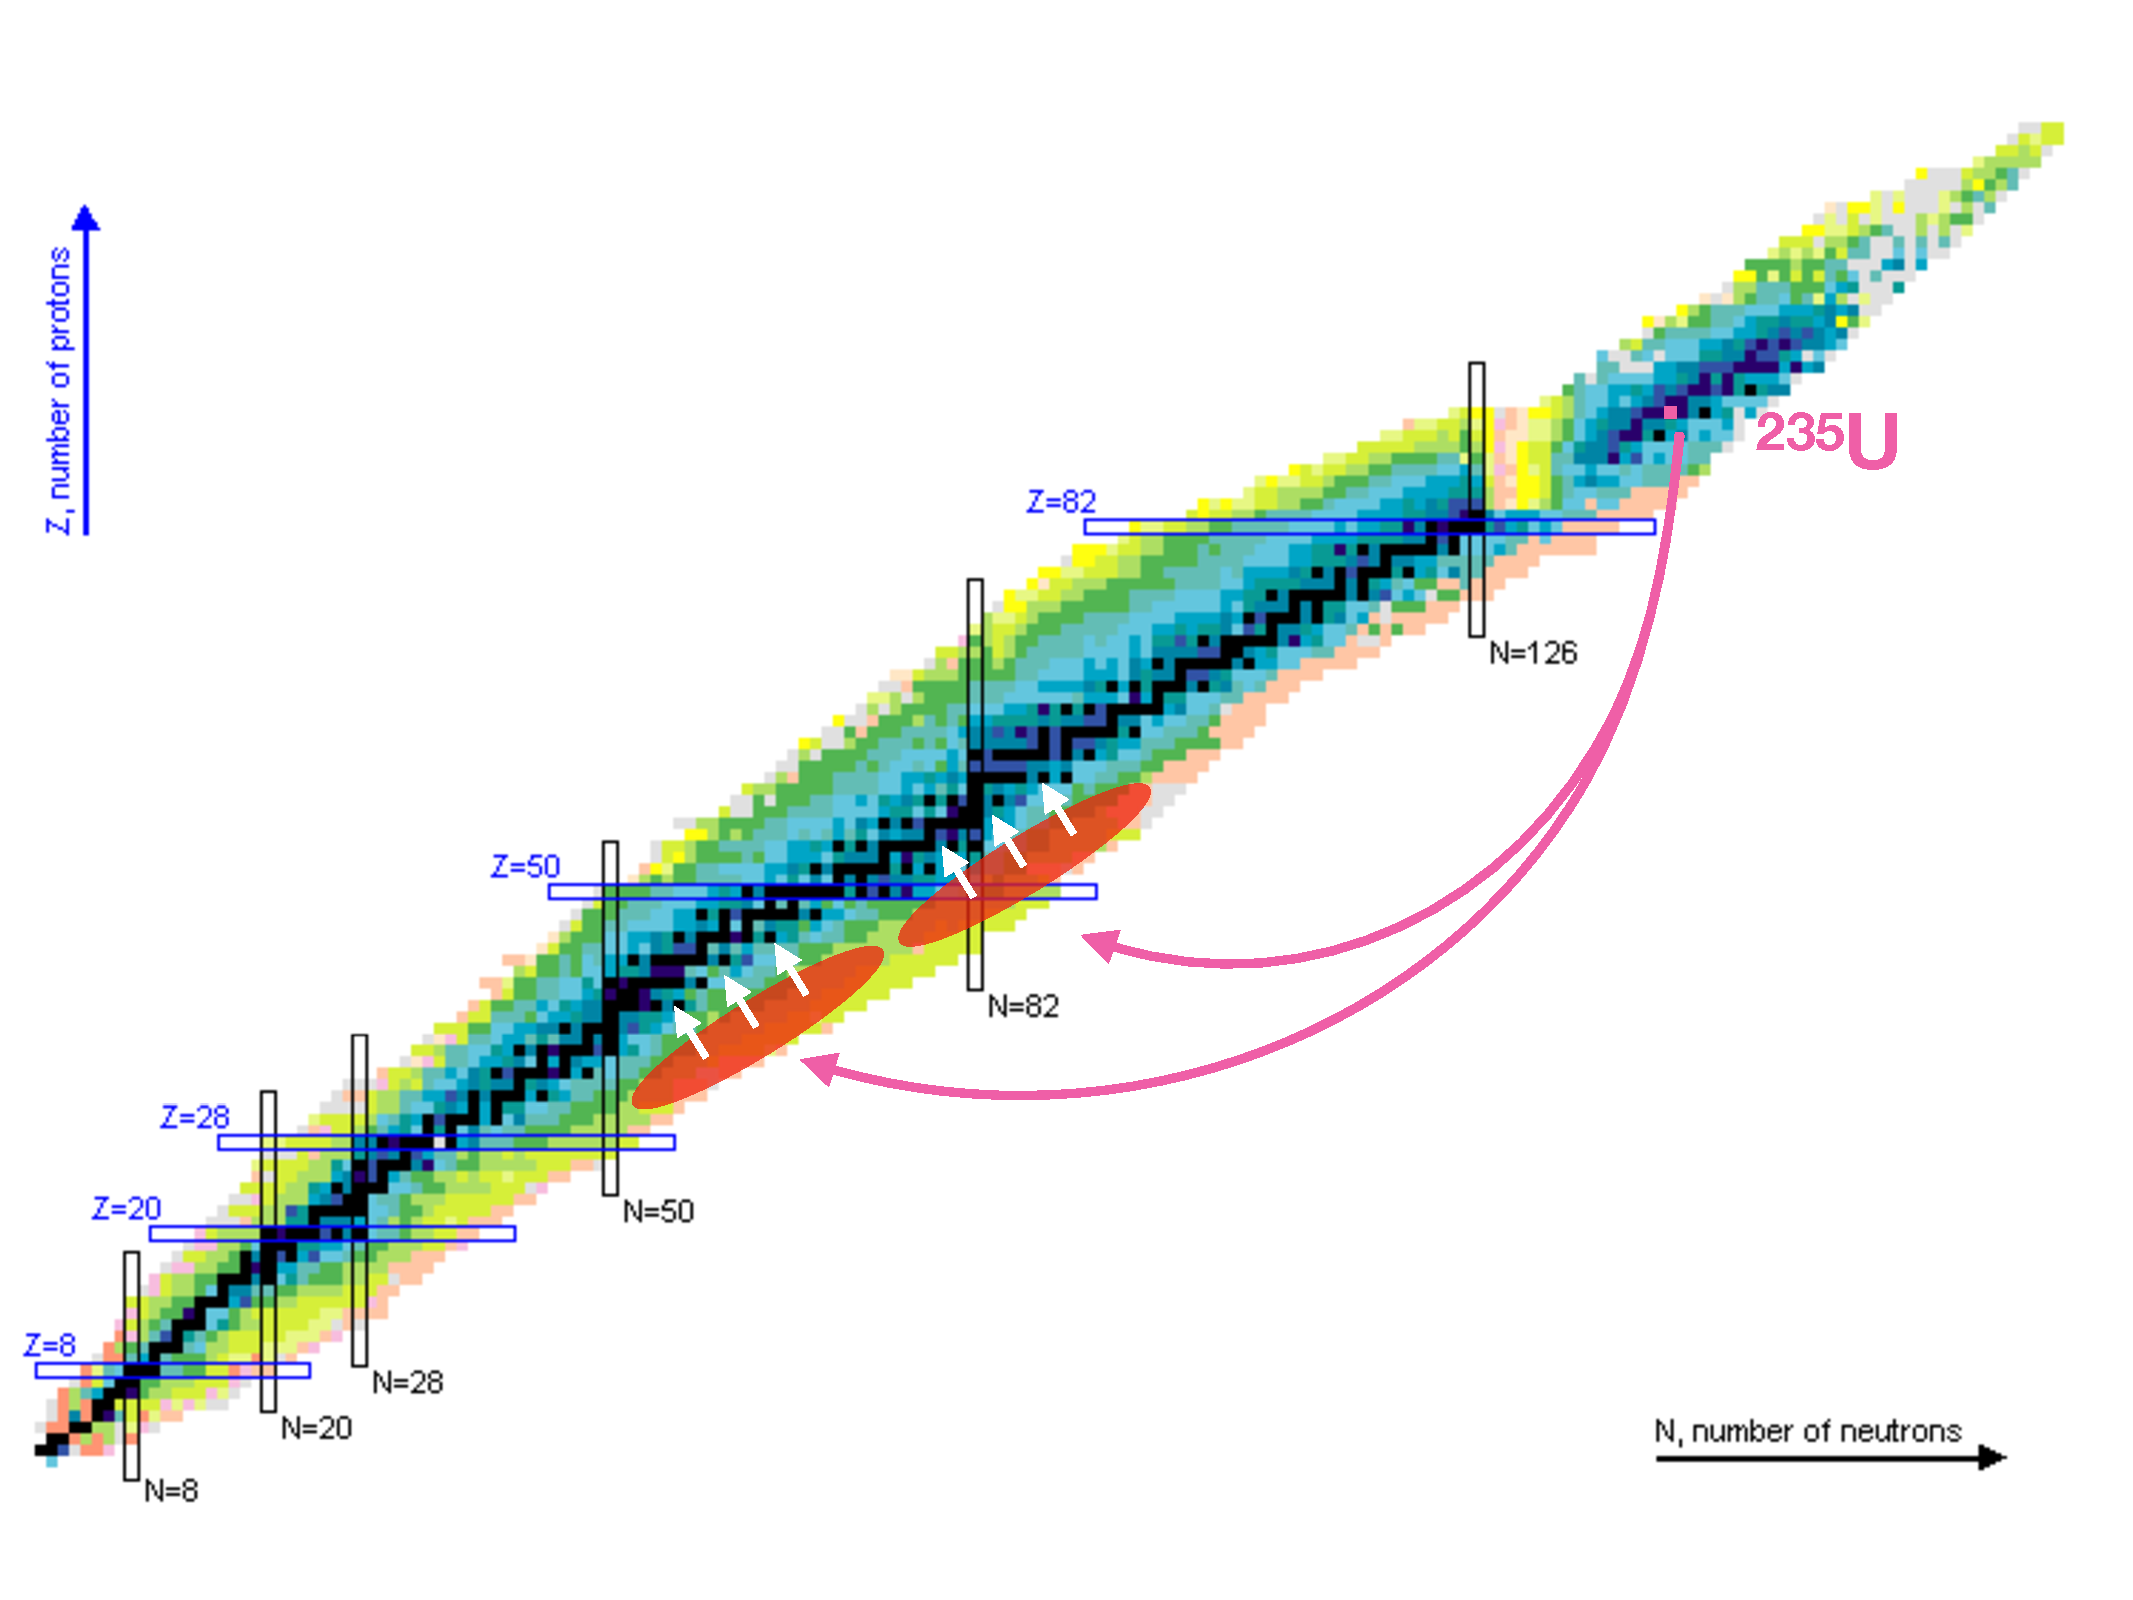
\includegraphics[width=0.7\linewidth]{tex/3-reactorneutrinos-images/NuclideChart_U235}
	\caption{A schematic of the fission of $^{235}$U \cite{NucChart}. After collision with a neutron $^{235}$U will split into two unstable nuclei (pink arrows) which will then $\beta$ decay (white arrows) until stable.}
	\label{fig:nucchart}
\end{figure}


\section{Measuring the Reactor Antineutrino Flux and Spectrum}

The total $\bar{\nu_{e}}$ flux, $S(E_\nu)$, produced by a nuclear reactor can be expressed as the sum over the spectra of the dominant fissioning isotopes,
\begin{equation}
	S(E_\nu) = \frac{W_{th}}{\sum_{i}(f_i/F)e_i}\sum_{i}\frac{f_i}{F}\left(\frac{dN_i}{dE_\nu}\right) ,
\end{equation}
where $f_i/F$ is the fission fraction for each given isotope $i$, $W_{th}$ is the reactor thermal energy, $e_i$ is the 
average energy released per fission by each isotope, and $dN_i/dE_\nu$ is the cumulative $\bar{\nu_e}$ spectrum of $i$ normalized per fission.

There are two methods to determine the $\bar{\nu_e}$ spectrum, \textit{ab initio} summation and electron spectrum conversion.
In the \textit{ab initio} approach the spectrum is determined by summing the contributions of all $\beta$-decay branches of all fission fragments,
\begin{equation}
	\frac{dN_i}{dE_{\bar{\nu}}} =  \sum_{n}Y_n(Z,A,t)\sum_{n,i}b_{n,i}(E^i_0)P_{\bar{\nu}}(E_{\bar{\nu}},E^i_0,Z) ,
\end{equation}
where $Y_n(Z,A,t)$ is the number of $\beta$ decays of the fission fragment $Z, A$ at time $t$, $b_{n,i}(E^i_0)$ are the branching ratios with endpoint energies $E^i_0$, and $P_{\bar{\nu}}(E_{\bar{\nu}},E^i_0,Z)$ is the normalized $\bar{\nu_e}$ spectrum for the branch $n, i$.
This method relies on nuclear databases, such as the Evaluated Nuclear Data File (ENDF) and Joint Evaluated Fission and Fusion (JEFF) databases, for information about the branching ratios and decay energies. 
The antineutrino spectrum for the four main reactor isotopes calculated using \textit{ab initio} summation was done in Ref.~\cite{HayesVogel} and the result can be seen in Figure~\ref{fig:spectrum}. 

Though seemingly straightforward, this approach comes with some caveats.
The shear number of daughter isotopes ($>$1000) and individual $\beta$ decay branches ($>$6000) make the summation non-trivial.
This, along with the fact that not all branching ratios are known, and that the fission yields have been determined by several different database groups but don't always agree and have large uncertainties bring into question the validity of using only this method. 

\begin{figure}[t]
	\centering
	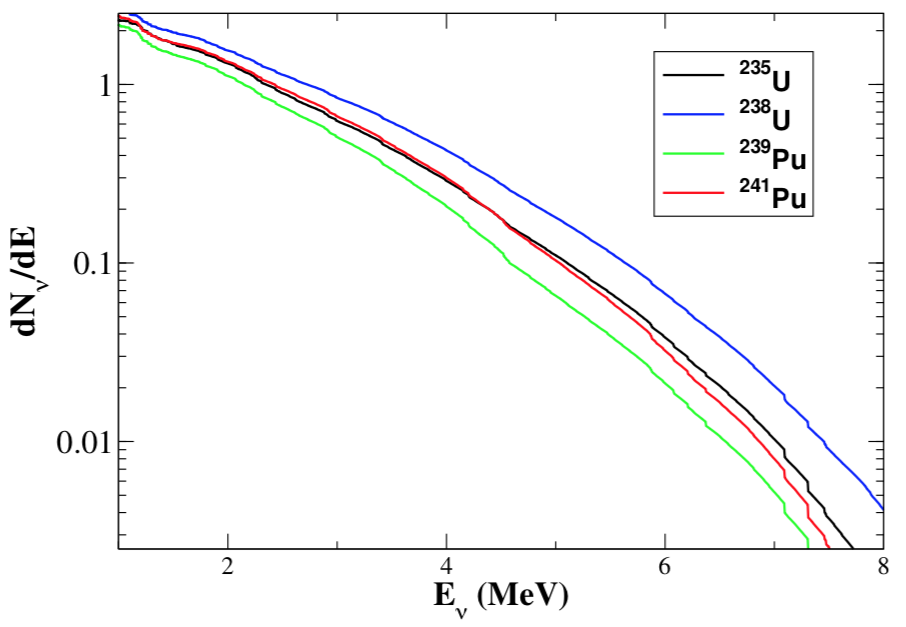
\includegraphics[width=0.65\linewidth]{tex/3-reactorneutrinos-images/Spectrum}
	\caption{The $\bar{\nu_e}$ spectrum predicted by the summation method using the JEFF-3.1.1 database fission fragment yields and the ENDF/B-VII.1 decay library \cite{HayesVogel}.}
	\label{fig:spectrum}
\end{figure}

The other approach to determine the $\bar{\nu_{e}}$ spectrum, the conversion method, relies on converting a measured electron spectrum into an antineutrino spectrum. 
This involves fitting an experimentally defined total beta spectrum with individual beta spectrum  according to their amplitudes, $a_i$, 
\begin{equation}
	\frac{dN_i}{dE_e} = \sum_{i}a_iP(E,E^i_0,Z)
\end{equation}
The conversion to the antineutrino spectrum is then accomplished by replacing the energy $E_e$ in each branch by $E_0 - E_{\bar{\nu}}$, because the electron and the $\bar{\nu_e}$ share the total energy of each $\beta$-decay branch.
The flux per fission is then given as the sum of $\bar{\nu_e}$ spectrum converted from each virtual $\beta$ branch,

\begin{equation}
	\frac{dN_i}{dE_{\bar{\nu}}} = \sum_{i}a_iP(E^i_0-E,E^i_0)
\end{equation}

%\begin{figure}
%	\centering
%	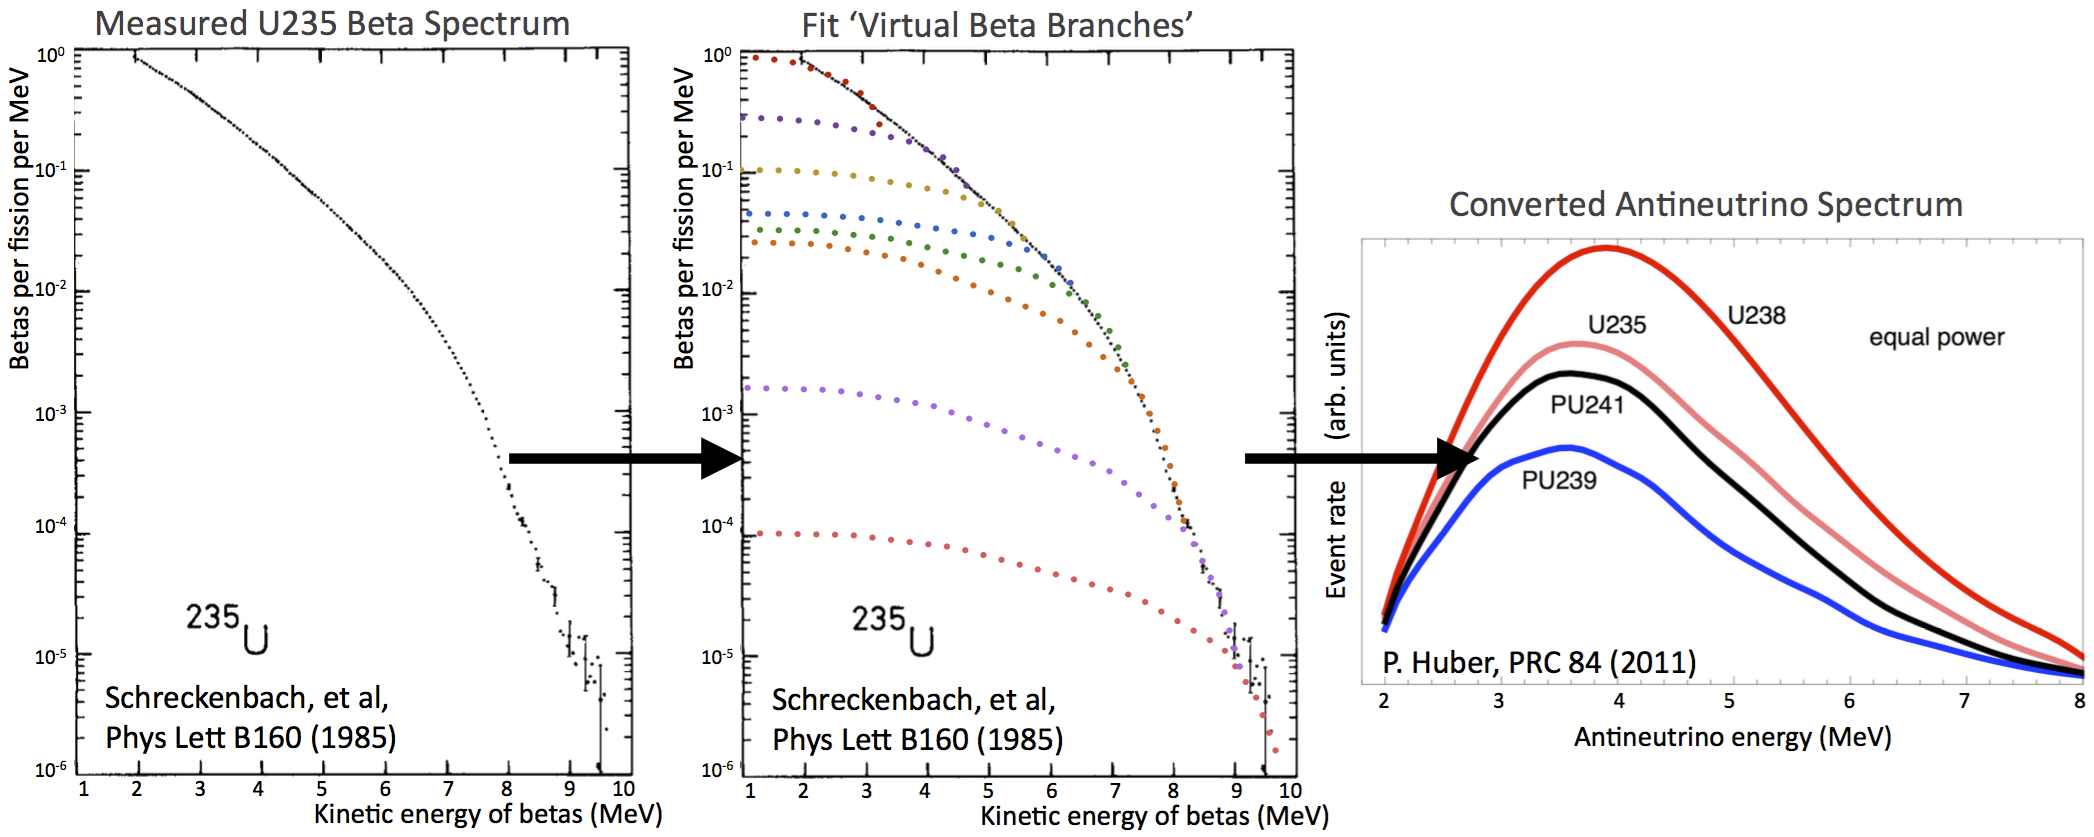
\includegraphics[width=0.7\linewidth]{tex/3-reactorneutrinos-images/betaspecconversion_fixed}
%	\caption{}
%	\label{fig:betaspecconversionfixed}
%\end{figure}

The electron spectra for $^{235}$U, $^{239}$Pu, and $^{241}$Pu were measured at the Institut
Laue-Langevin (ILL) reactor in Grenoble, France in the 1980s \cite{VonFeilitzsch:1982jw,Schreckenbach:1985ep,Hahn:1989zr}, while the spectrum of $^{238}$U was more recently (2014) measured at the neutron source FRMII in Garching, Germany \cite{Haag:2013raa}.
The ILL measurements, along with a prediction of the $^{238}$U $\bar{\nu_{e}}$ spectrum using the summation method by Vogel \cite{PhysRevC.24.1543}, became known as the ``ILL-Vogel" flux model and was the main model used until 2011.

In 2011 Mueller \textit{et al.} improved the prediction of the reactor antineutrino spectra by employing a method that combined information from the nuclear databases and the measured electron spectra from ILL \cite{Mueller}. 
This was followed by a further improvement by Huber who applied higher order corrections making use of the conversion method and minimizing the use of the databases as much as possible \cite{Huber}.

Though much work has been done to accurately model the reactor antineutrino spectra both methods are subject to uncertainties in the subdominant corrections to beta-decay. This includes radiative, weak magnetism, and finite size corrections along with uncertainties in the spectrum shape of forbidden transitions which are summarized in Ref.\cite{HayesVogel}. 
Besides the model uncertainties there are also experimental uncertainties that come from knowing the thermal power of the reactor, its time-dependent fuel composition, and the fission energies of the dominant isotopes.
All of this results in a 10-20\% relative uncertainty on the reactor antineutrino spectra using the \textit{ab initio} method and $\sim$5 \% uncertainty on the conversion approach \cite{Qian:2018wid}.



\section{Detection of Reactor Neutrinos}

Though there are several methods that can be used to detect reactor neutrinos, including charge-current ($\bar{\nu_e} + d \rightarrow n + n + e^+$), neutral-current ($\bar{\nu_e} + d \rightarrow n + p + \bar{\nu_e}$), and antineutrino-electron elastic scattering ($\bar{\nu_e} + e^- \rightarrow \bar{\nu_e} + e^-$), the one employed by most experiments is IBD ($\bar{\nu_e} + p \rightarrow e^+ + n$).
The IBD reaction energy threshold is 1.8 MeV and the cross section is relatively high, $\sim 63 \times 10^{-44} \textrm{cm}^2/\textrm{fisson}$ integrated over the entire reactor neutrino energy spectrum \cite{Qian:2018wid}, and can be written as
\begin{equation}
	\sigma^{(0)} \simeq 9.52 \times \left(\frac{E_e^{(0)}p_e^{(0)}}{\textrm{MeV}^2}\right) \times 10^{-44}\textrm{cm}^2
\end{equation}
where $E_e$ and $p_e$ are the energy and momentum of the final-state positron. 

An IBD event is selected by a pair of coincident signals consisting of a positron ionization and annihilation as the prompt signal and a time delayed neutron capture on a proton or nucleus as the delay signal. 
The neutron energy can be backtracked from the prompt signal as
\begin{equation}	
	E_{\bar{\nu}} = E_{prompt} + 0.78~\textrm{MeV} + T_n
\end{equation}
where $T_n$ is the kinetic energy of the recoil neutron which is much smaller than the energy of the neutrino and can therefore be ignored in most cases. 
The IBD cross-section increases with energy, whereas the $\bar{\nu_{e}}$ spectrum decreases with energy creating a detected energy spectrum that peaks around 3.8 MeV and dies off after $\sim$8 MeV, as seen in Figure~\ref{fig:vogel-fig02}. 

In addition to great background rejection and good reconstruction of the neutrino energy, the IBD method of detecting neutrinos also allows the use of liquid scintillators and water as detection mediums. 

\begin{figure}[h]
	\centering
	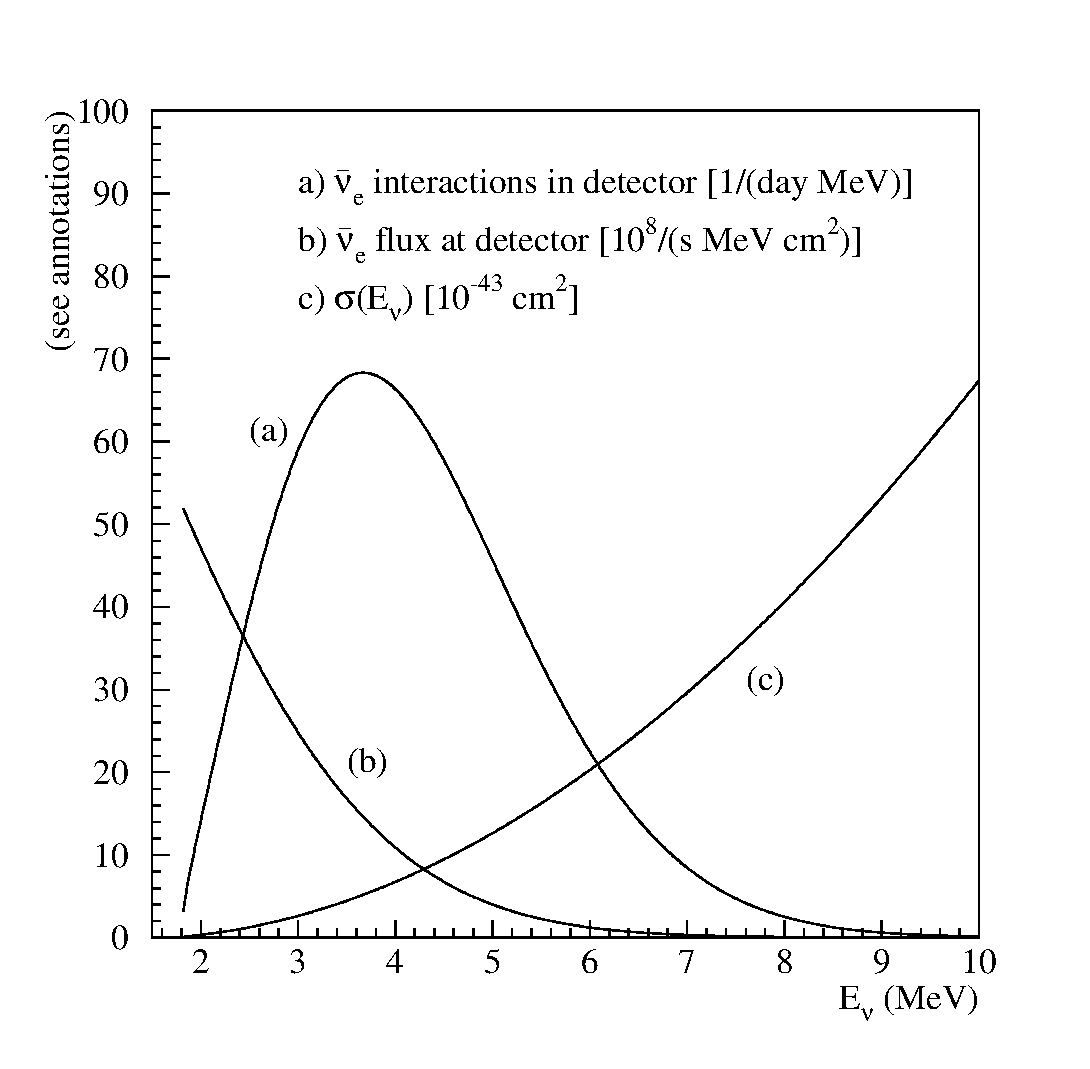
\includegraphics[width=0.5\linewidth]{tex/3-reactorneutrinos-images/vogel-fig02}
	\caption{The IBD spectrum (curve (a)) measured by a 12-ton fiducial mass detector located 0.8 km from a 12-GW$_{th}$ power reactor along with the reactor flux (curve (b)) and IBD cross section (curve (c)) as a function of energy \cite{PDG}.}
	\label{fig:vogel-fig02}
\end{figure}




\section{The Reactor Antineutrino Anomaly}







\chapter{\uppercase{Sterile Neutrinos}}

\section{Theory of Sterile Neutrinos}

\section{Experimental Searches for Sterile Neutrinos}


\chapter{PROSPECT}

\section{Motivation}

\section{Experimental Site}

\section{Design}

\section{Detecting Inverse Beta Decays}

\section{From Signal to Result}



\chapter{\uppercase{$^{227}$Ac as a Calibration Source}} \label{ch:Ac}

\section{Motivation}

In the absence of an eV-scale sterile neutrino PROSPECT would measure IBD rates that fall like one over distance from the reactor squared. 
If sterile neutrino oscillation was detected, after one year, PROSPECT would measure something similar to the oscillation signature seen in Figure~\ref{fig:lovere1yr}, given a mass splitting of 1.78~eV$^2$ and an oscillation amplitude of 0.09, which is close to the Reactor Antineutrino Anomaly best-fit point (see Figure~\ref{fig:raabestfitpoint}).
\begin{figure}[!b]
	\centering
	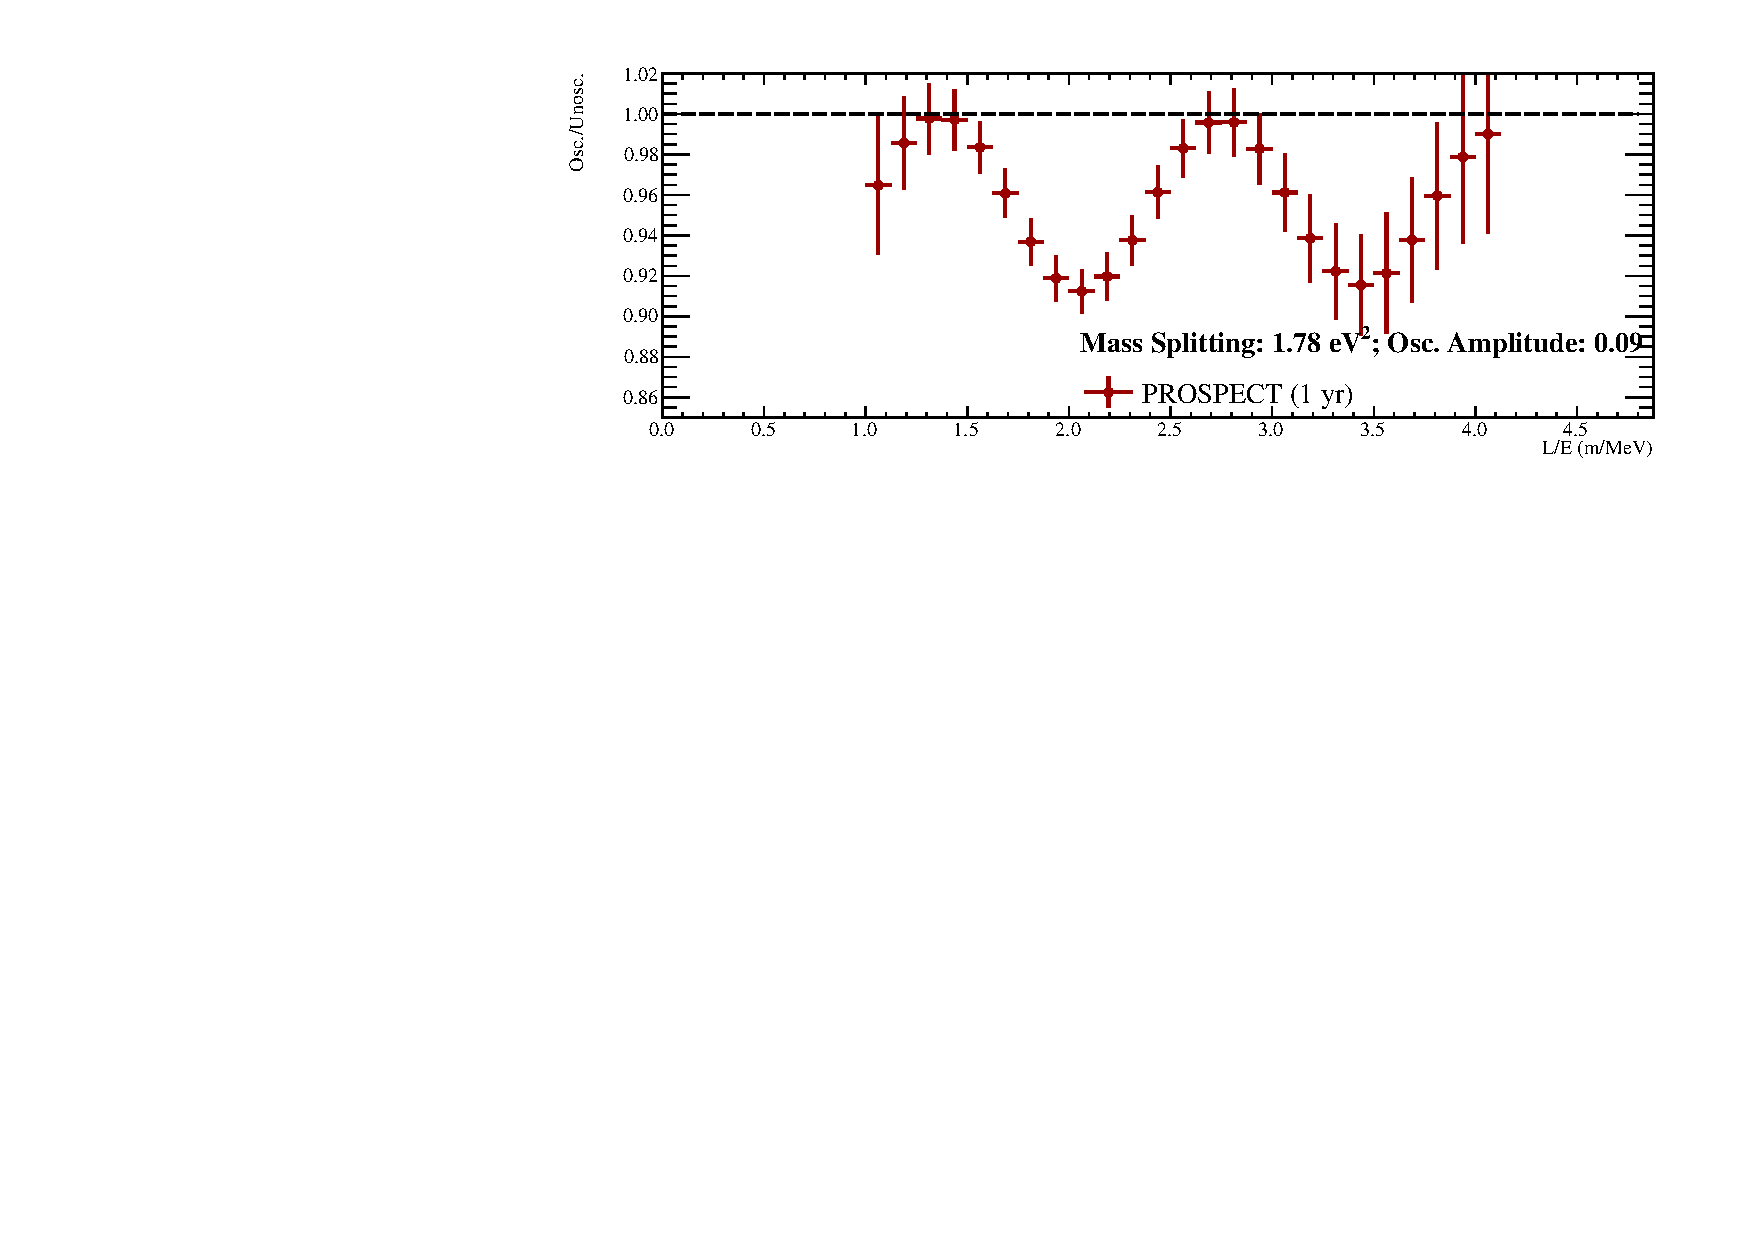
\includegraphics[width=0.7\linewidth]{tex/6-ac227-images/LoverE_1yr}
	\caption{The ratio of the oscillated to un-oscillated neutrino spectrum as a function of L/E that would be observed by PROSPECT after 1 year if a sterile neutrino signal was detected \cite{PSurukuchi:1534}.}
	\label{fig:lovere1yr}
\end{figure}
Given that the oscillation signal in PROSPECT is a deviation from an expected 1/$r^2$ neutrino rate fall-off with distance from the reactor, it is crucial to ensure that relative segment-to-segment volume variations do not mimic this signal.

Relative segment volumes can be measured via an event source uniformly distributed throughout the active volume of the detector. 
This was accomplished in PROSPECT by mixing a radioactive isotope, \Ac, with the liquid scintillator and using measured decay rates as a proxy for segment volume.

We chose \Ac for several reasons. First, because an \AaAa coincidence occurs in its decay chain, specifically $^{219}$Rn $\rightarrow ^{215}$Po + $\alpha \rightarrow ^{211}$Pb + \Aa, as highlighted in Figure~\ref{fig:ac227chain}.
\begin{figure}[!b]
	\centering
	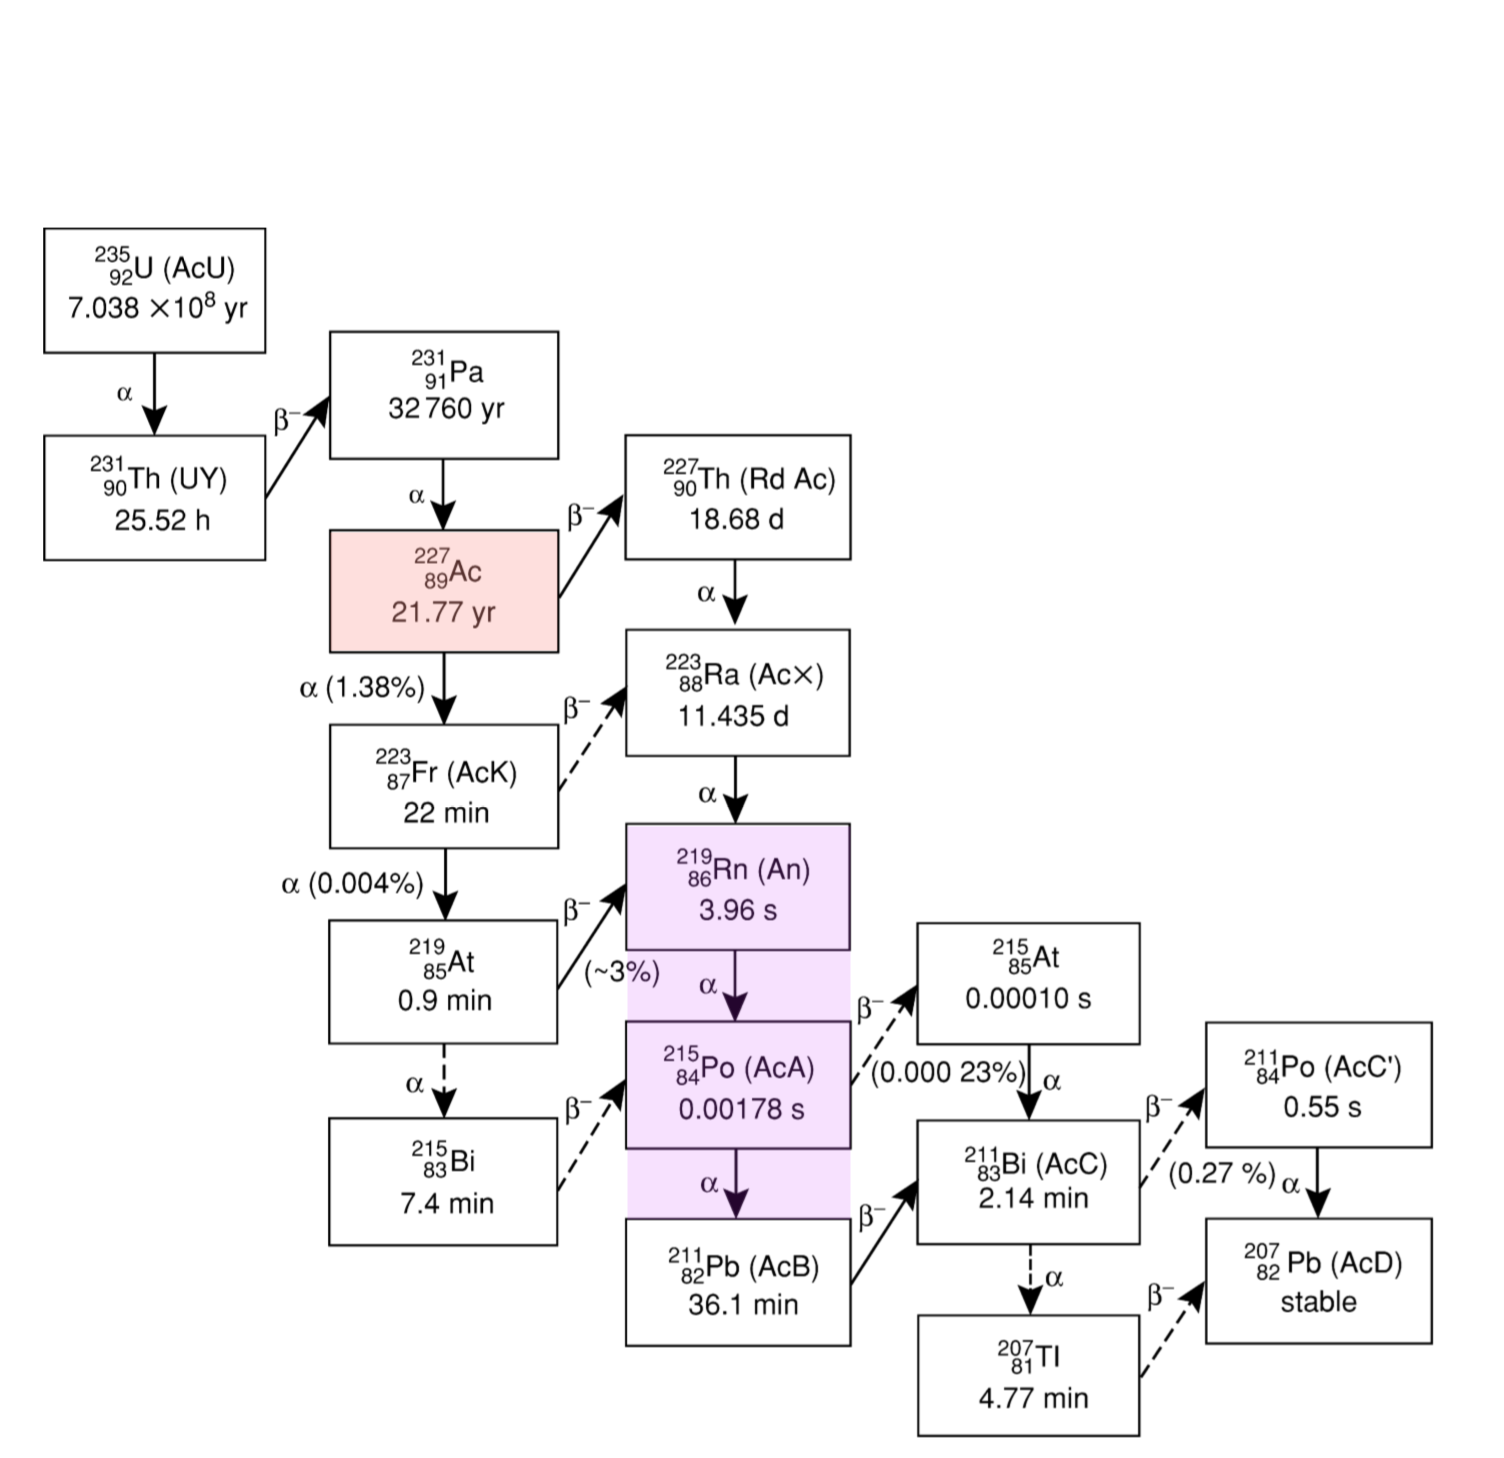
\includegraphics[width=0.6\linewidth]{tex/6-ac227-images/Ac227Chain}
	\caption{The full decay chain of \Ac (a daughter of $^{235}$U), in which the \AaAa coincidence of interest is highlighted \cite{Kirby2011}.}
	\label{fig:ac227chain}
\end{figure}
\Rn has a half-life of 3.96 $\pm$ 0.01 s and $\alpha$-decays 100\% of the time, while \Po has a half-life of 1.781 $\pm$ 0.005 ms and $\alpha$-decays  99.99977(2)\% of the time \cite{ENSDF}.
The \Aa decay of \Po (see Figure~\ref{fig:215poalphadecay}) is mono-energetic at 7.39 MeV which results in a $\sim$0.78 MeV$_{ee}$\footnote{Due to quenching in the scintillator that causes suppressed light output, the observed energy is sometimes referred to as electron-equivalent energy.} signal in the PROSPECT detector after quenching, well removed from nLi captures on $^6$Li (the delayed signal used for neutrino identification) that occur around 0.5 MeV$_{ee}$. 
In addition, there are no corresponding gammas with the \Po decay, making this a very clean and well defined signal.
The \Rn \Aa decays (see Figure~\ref{fig:219rnalphadecay}) are not as clean, with the alpha having a non-negligible probability of decaying to 3 excited states of the daughter in addition to the ground state and thus producing accompanying gamma rays, as listed in Table~\ref{tab:RnPoE}. 
The use of time, energy, and PSD cuts, though, make them easy to pair with corresponding \Po decays.

\begin{table}[!t]
	\centering
\begin{tabular}{|c|c|c|c|c|c|}
	\hline 
	& E$_\alpha$ [keV] & I$_\alpha$ \% &  & E$_\gamma$ [keV] & I$_\gamma$ \% \\ 
	\hline 
	\Rn & 6425.0(10) & 7.5(6) &  & 271.23(1) & 10.8(6) \\ 
	%\hline 
	& 6530(2) & 0.110(10) &  & 401.81(1) & 6.6(4) \\ 
	%\hline 
	& 6552.6(10) & 12.9(6) &  & 130.60(3) & 0.13(9) \\ 
	%\hline 
	& 6819.1(3) & 79.4(10) &  &  &  \\ 
	\hline 
	\Po & 7386.1(8) & 99.999770(20) &  &  &  \\ 
	\hline 
\end{tabular} 
\caption{Energy and absolute intensity of dominant $\alpha$ and $\gamma$ decay radiation for \Rn and \Po. Decay energies not listed here have an intensity of $< $0.05\%.}
\label{tab:RnPoE}
\end{table}

Another reason \Ac is an attractive source is its long half-life, 21.77 years, ensuring that the rate of RnPo \footnote{Short-hand used to refer to the event selection of the  $^{219}$Rn $\rightarrow ^{215}$Po + $\alpha \rightarrow ^{211}$Pb + \Aa chain} events remains close to constant over the lifetime of the detector.
It is also important that the chosen source is in equilibrium with its decay products at the time of use so that constant rates can be measured.
It takes about 188 days for \Ac to come into equilibrium with its decays products \cite{DBerish:597}, and given the probable amount of time that would pass between obtaining the source and adding it to the liquid scintillator in the detector, it was assumed that equilibrium would be reached. 

The ability to select RnPo events using a time coincidence analysis means that only a small amount of \Ac needs to be added to the liquid scintillator. 
This is useful because it is important that no significant additional backgrounds be added to the already large backgrounds present.
It should also be noted that $\alpha$'s deposit their energy in the scintillator within a few tens of microns, resulting in a highly localized signal. 
This also means that all RnPo events occur in the same segment, providing another handle that can be used in the event selection.

\begin{figure}[H]
	\centering
	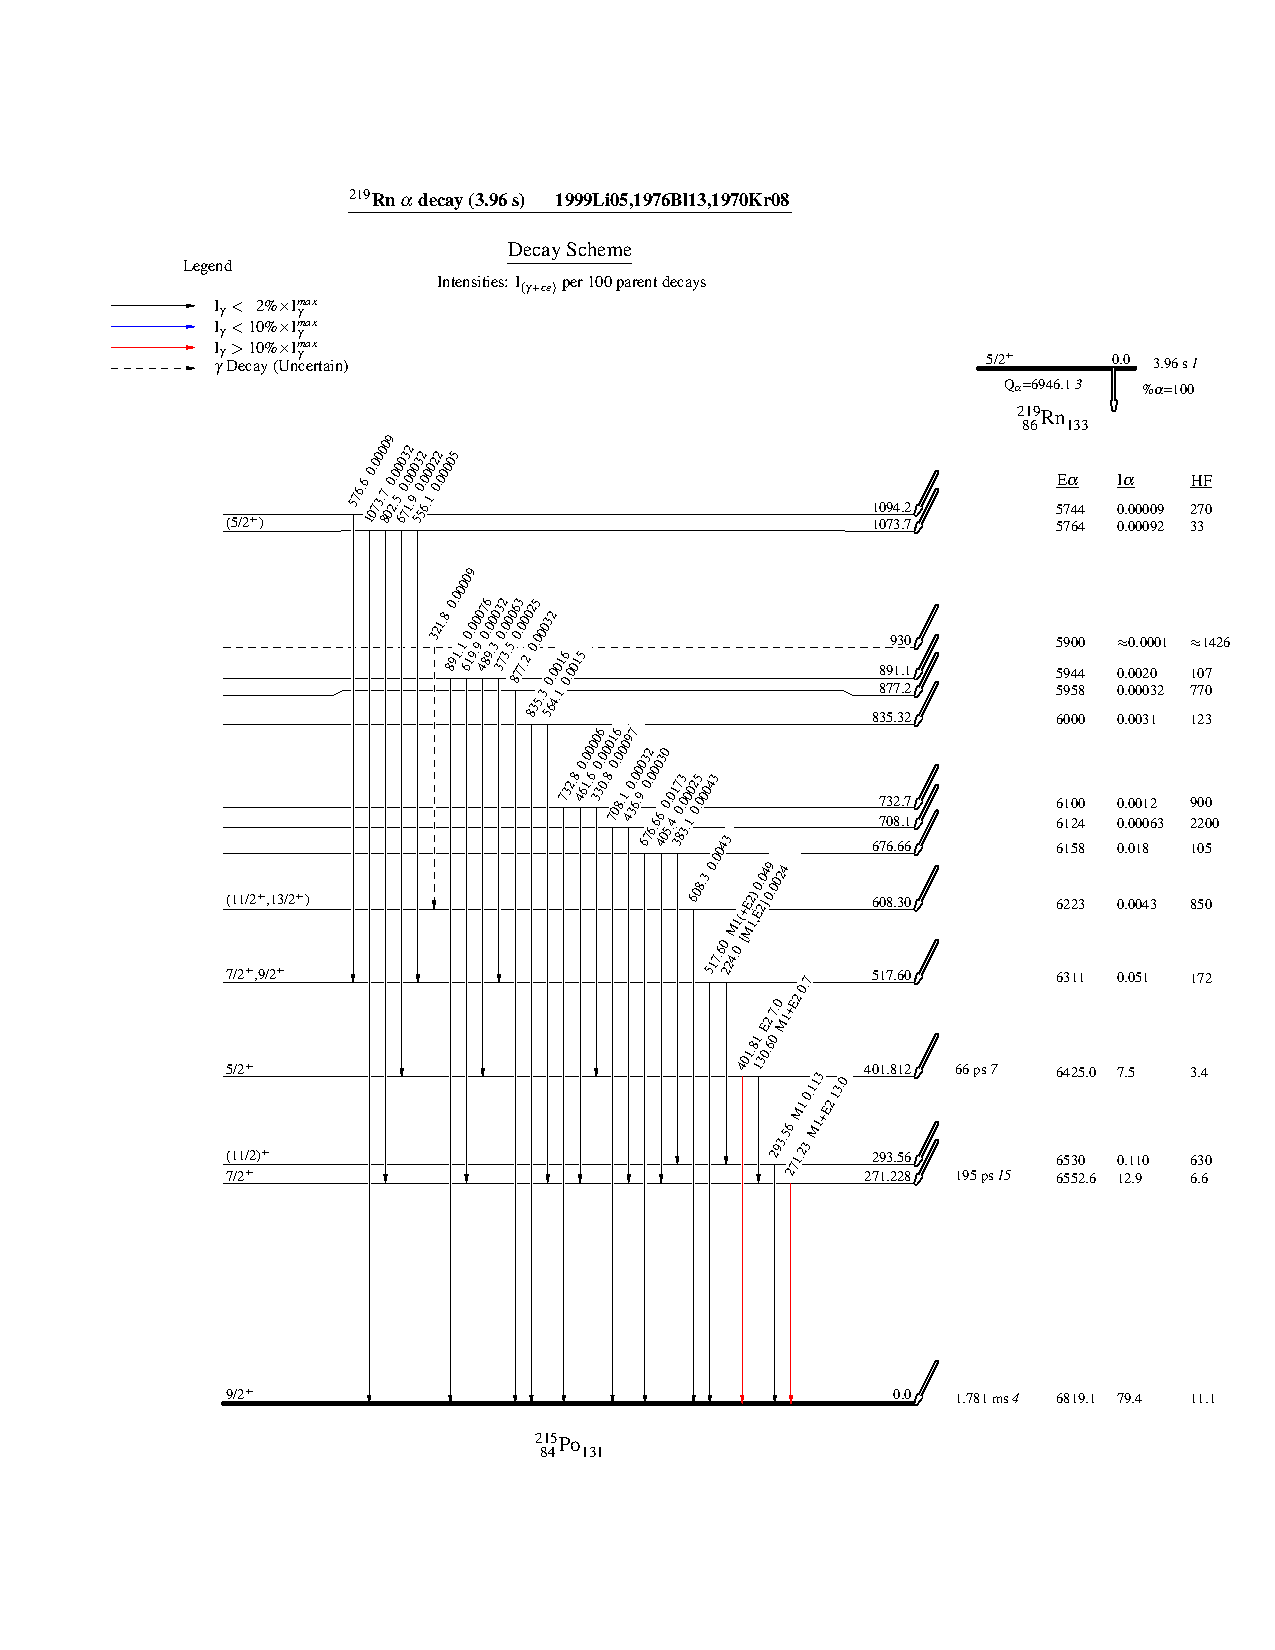
\includegraphics[width=0.95\linewidth]{tex/6-ac227-images/219RnAlphaDecay}
	\caption{The decay scheme of \Rn \cite{ENSDF}.}
	\label{fig:219rnalphadecay}
\end{figure}

\begin{figure}[H]
	\centering
	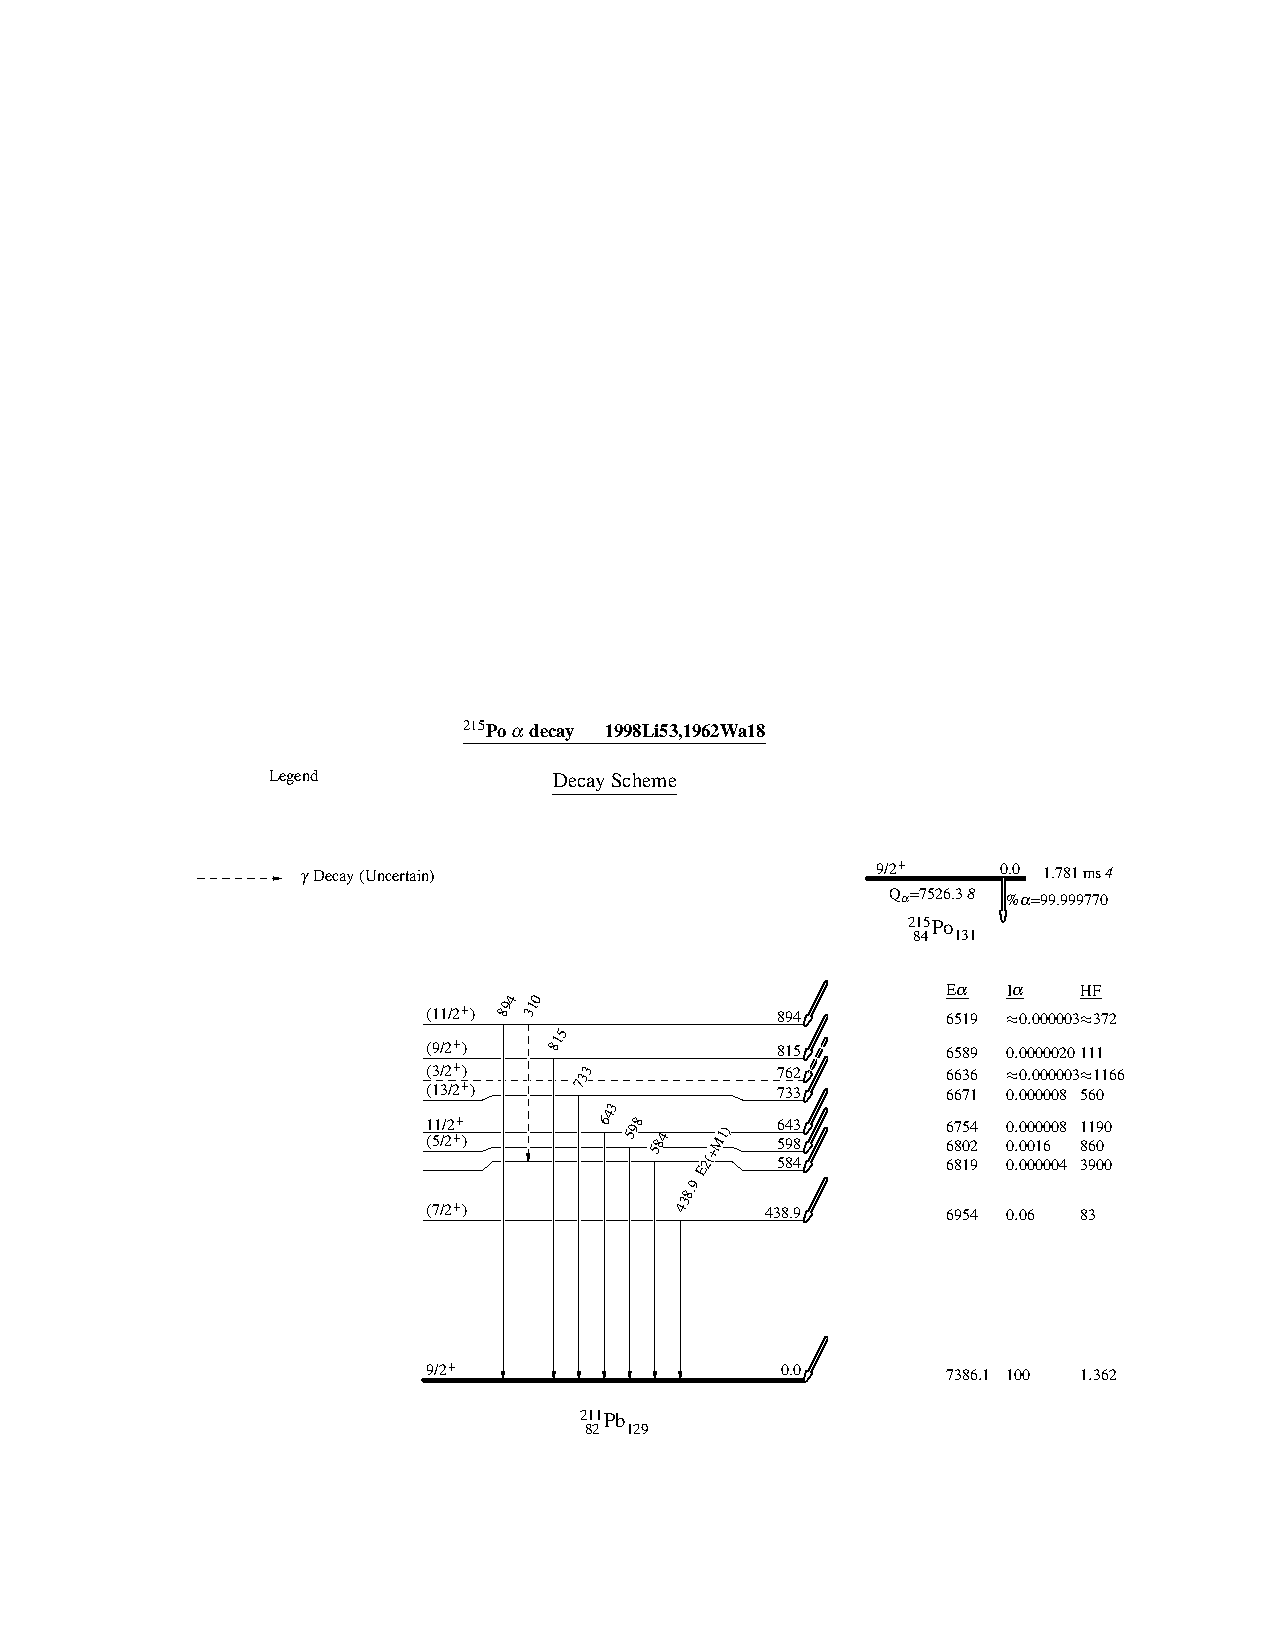
\includegraphics[width=0.95\linewidth]{tex/6-ac227-images/215PoAlphaDecay}
	\caption{The decay scheme of \Po \cite{ENSDF}.}
	\label{fig:215poalphadecay}
\end{figure}


\newpage
\section{Material Compatibility}

Before \Ac could be added to the PROSPECT detector, it had to be determined that \Ac and its daughters would not adsorb onto detector materials and that it would not degrade the scintillator.
If it was adsorbed then it would not be a uniform source in the detector, nullifying the ability to use measured decay rates as a proxy of volume.
To test this six material samples were placed in vials of identically prepared $^6$Li-LS spiked with $^{227}$Ac. The rate of \Ac in each sample vial and one reference vial with no material was measured and tracked over a period of 6 months. 
An observation of a significant decrease in rate, relative to the half-life of \Ac, would indicate that \Ac was adsorbing onto the material.

\subsection{Material and Scintillator Preparation}
The materials tested were: ultraviolet transmitting (UVT) acrylic, flourinated ethylene propylene (FEP), polylactide (PLA), polyether ether ketone (PEEK), a RG 188 cable, and viton o-rings. See Table~\ref{tab:materials} for a list of their uses in the detector and sample sizes.
To prepare the materials they were all placed in a single beaker with ultra-pure water and cleaned ultrasonically for 30 minutes.
They were then transferred to a watch glass and placed in a 50 C oven for two hours.
After drying they were placed in empty 12 ml vials.

The \Ac used to spike the scintillator was obtained from Eckert and Ziegler as a solution of 3.711$\times$10$^4$ Bq $\pm$ 1.32\% of \Ac in 10.22710 g of 1 M HCl, measured on September 6, 2016.
0.503 g of this solution was added to 192 g of $^6$Li-LS on December 15, 2016.
With an accepted half-life of 21.772 $\pm$ 0.003 yrs \cite{ENSDF}, the activity of the \Ac solution before adding to the LiLS was 36788 Bq, yielding a final activity of 94.2 Bq/10 g. 
This is the stock solution from which all LS was taken for the material studies and later on for spiking the detector.

Prior to filling all sample vials the threads of each vial were wrapped with teflon tape in an effort to obtain a secure seal. 
The reference vial was filled on December 15, 2016 with 10.030 g of \Ac spiked LiLS from the stock solution, yielding an expected activity of 94.5 Bq.
All material vials were filled on February 24, 2017 with the amount of stock solution added to each listed in Table~\ref{tab:MatFill}.
At the time of filling the rate in each vial was expected to be $\sim$93 Bq.
For a photograph of all filled material sample vials see Figure~\ref{fig:samples}.

\begin{table}[h]
	\centering
\begin{tabular}{|p{0.16\textwidth}|p{0.4\textwidth}|p{0.33\textwidth}|}
	\hline 
	\textbf{Material} & \textbf{Detector Use} & \textbf{Sample Size} \\ 
	\hline 
	UVT Acrylic & Front window of PMT housing & 1.0 $\times$ 1.15 $\times$ 0.1 cm$^3$ \\ 
	\hline 
	FEP  & Film on optical separators & 1.5 $\times$ 1.5 cm$^2$, 3 mm thick \\ 
	\hline 
	PLA & 3D printed pinwheels & 10 disks; 0.5 cm diameter, 0.1 cm thick \\ 
	\hline 
	PEEK & Seal plugs through which the high voltage and signal cables were threaded. Screws used to bolt together segment supports. Spacers at the base of the acrylic tank. & 1 Nut; ID 0.5 cm, small OD 1cm, large OD 1.1cm, thickness 0.5 cm \\ 
	\hline 
	RG188 Cable & High voltage and signal cables & 4.5'' long \\ 
	\hline 
	Viton O-ring & Seal back plugs of PMT housings and seal acrylic tank & 10 O-rings; OD 6mm, ID ~3mm, thickness 1.5mm \\ 
	\hline 
\end{tabular} 
\caption{Samples used to test if \Ac or its daughters would adsorb onto detector materials.}
\label{tab:materials}
\end{table}

\begin{table}[h]
	\centering
\begin{tabular}{|c|c|c|}
	\hline 
	\textbf{Material} & \textbf{Date Filled} & \textbf{LiLS Added (g)}  \\ 
	\hline 
	Reference & 12/15/2016 & 10.030 \\ 
	\hline 
	UVT Acrylic & \multirow{6}{*}{02/24/2017}  & 9.98 \\ 
	%\hline 
	FEP &  & 9.98 \\ 
	%\hline 
	PLA &  & 9.999 \\ 
	%\hline 
	PEEK &  & 9.99 \\ 
	%\hline 
	RG188 Cable &  & 9.981  \\ 
	%\hline 
	Viton O-ring &  & 10.011  \\ 
	\hline 
\end{tabular} 
\caption{The weight of \Ac spiked LiLS that was added to each sample vial.}
\label{tab:MatFill}
\end{table}

\begin{figure}[H]
	\centering
	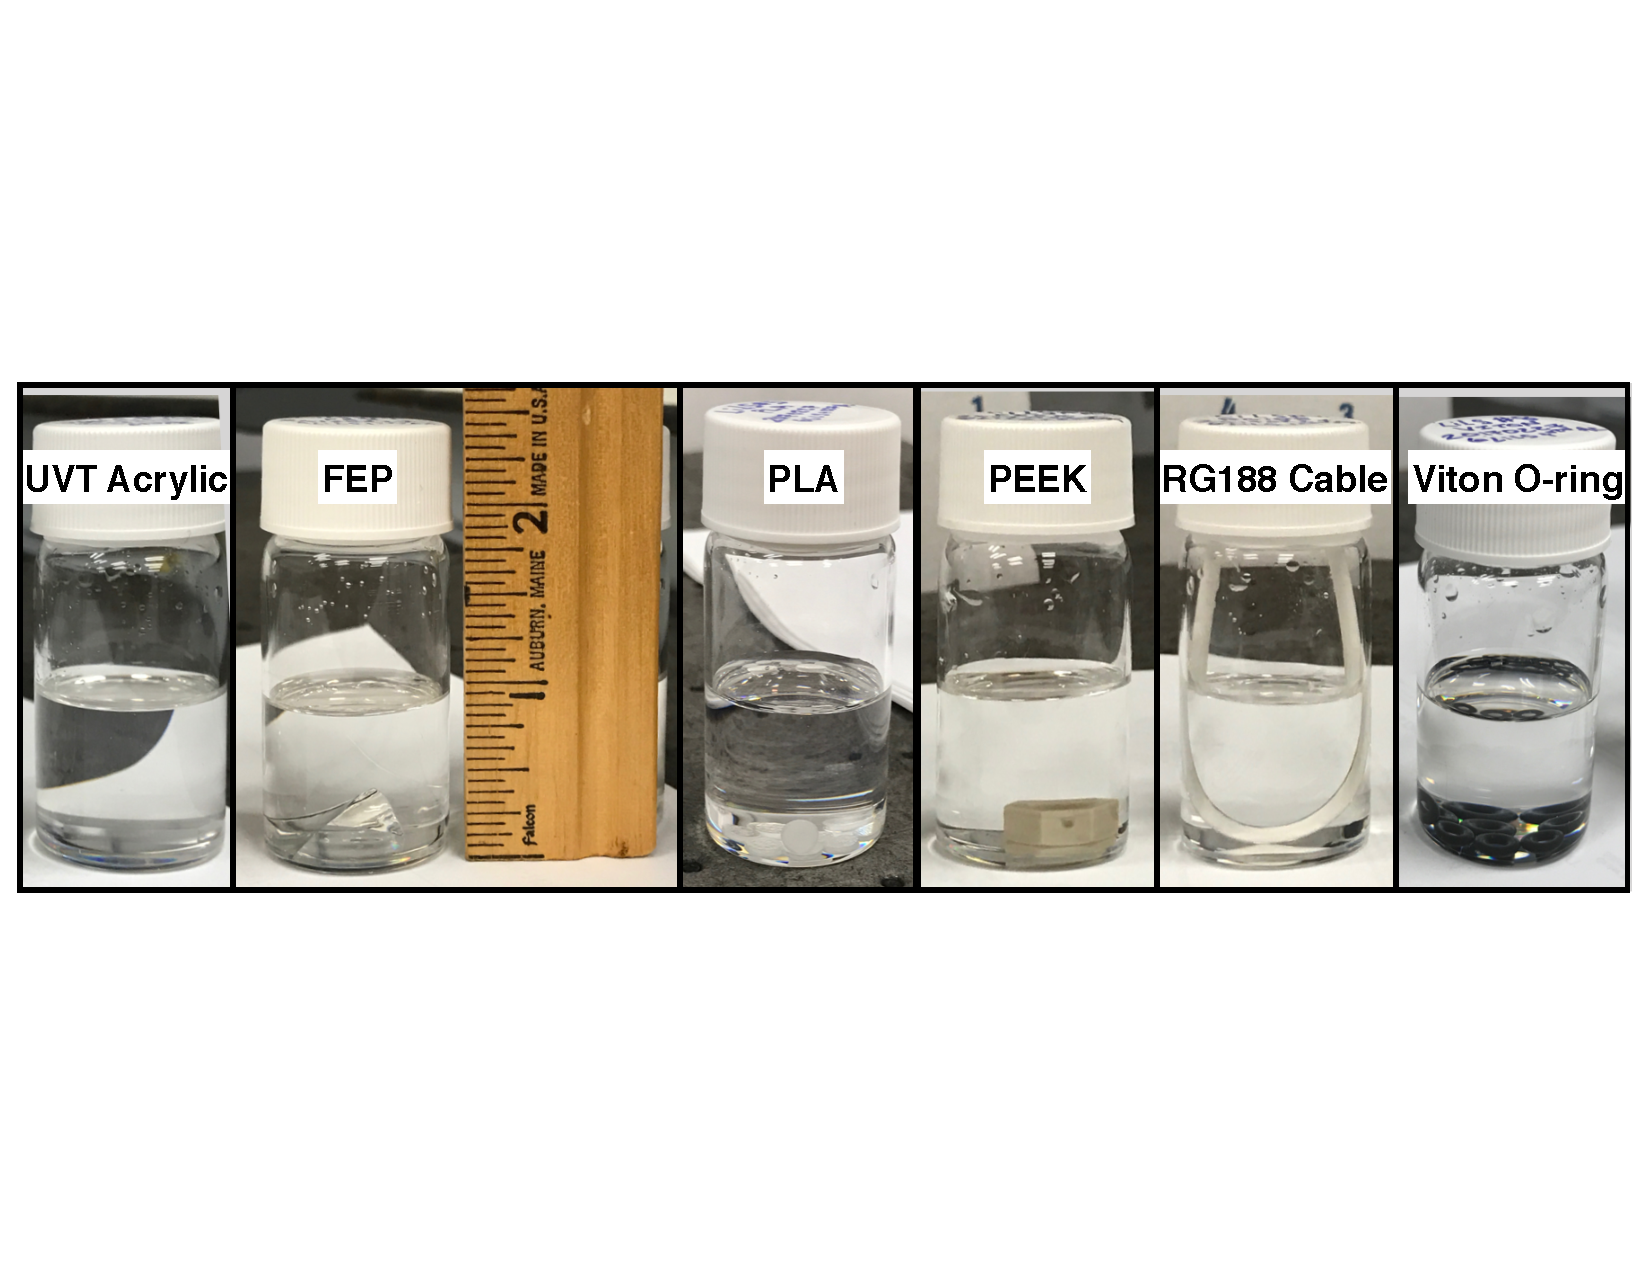
\includegraphics[width=0.8\linewidth]{tex/6-ac227-images/BNL/Samples}
	\caption{Photos of all material sample vials filled with \Ac spiked LiLS, with ruler for scale.}	
	\label{fig:samples}
\end{figure}

\subsection{Detector}

The detector consisted of a 2-inch photomultiplier tube coupled using optical grease to a solid cylinder of UVT acrylic painted with reflective white paint with an insert cut out to hold the sample vials, as shown in Figure~\ref{fig:blackbox}.
Placed in a dark box the PMT was cabled to a CAEN DT55xx Desktop HV Power Supply and a CAEN DT5730 8 Channel 14-bit 500 MS/s Digitizer \cite{CAENDigit}.
A modified version of Wavedump 3.7.2 \cite{CAENWD} was used to start and stop the data runs and save the waveforms of the signals.

\begin{figure}[H]
	\centering
	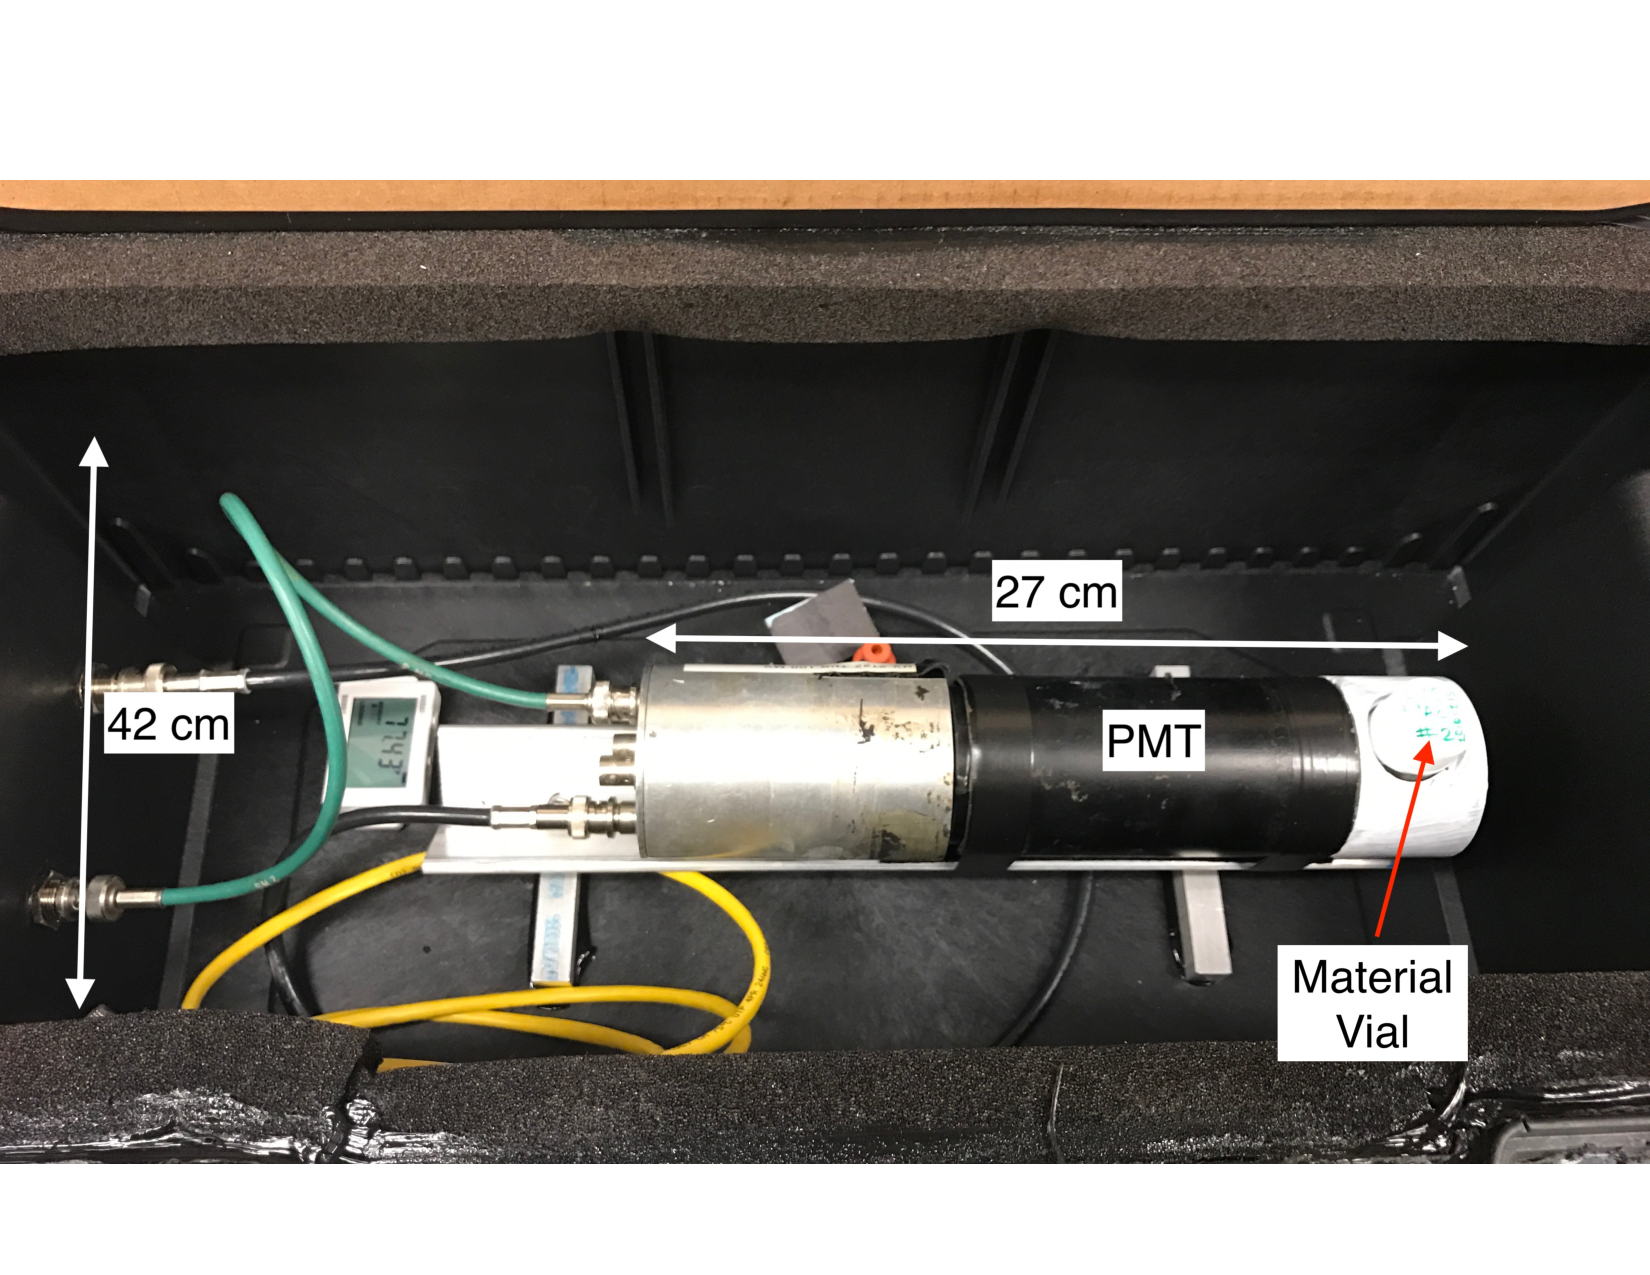
\includegraphics[width=0.65\linewidth]{tex/6-ac227-images/BNL/BlackBox}
	\caption{Detector used for material studies, consisting of a 2-inch PMT coupled to an acrylic cylinder holding the sample vials, all contained in a dark box. The PMT is cabled to a power supply and digitizer that exist outside of the box.}
	\label{fig:blackbox}
\end{figure}

\subsection{Data Analysis}

The raw waveforms were analyzed to calculate the energy and PSD of each signal. 
Each collected waveform consisted of 250 2 ns samples.
The energy was measured by taking the integral of the waveform using the trapezoidal rule in ADC units.
The total energy was converted to nC using
\begin{equation}
E[nC] = E[ADC] \times \frac{1\times10^9}{R\times\textrm{sample-rate}\times n[ADC/V]},
\end{equation}
where $R$, the resistance, is 50 $\Omega$, the sample-rate is $5\times10^8$ Hz, and $n = (2^{14} -1)/2 = 8191.50$ ADC/V, because we used a 14 bit ADC with a 2 V range.
The tail and total fractions used to calculate the PSD were both measured from the leading half-minimum point of the negative pulses.
The total pulse area was measured as the integral from 10 samples before the half-min to 140 samples after.
The tail area was measured as the integral from 19 samples after the half-max to 140 samples after.
For an example of this for a typical alpha signal in the reference sample see Figure~\ref{fig:waveformbnl}.

\begin{figure}[!t]
	\centering
	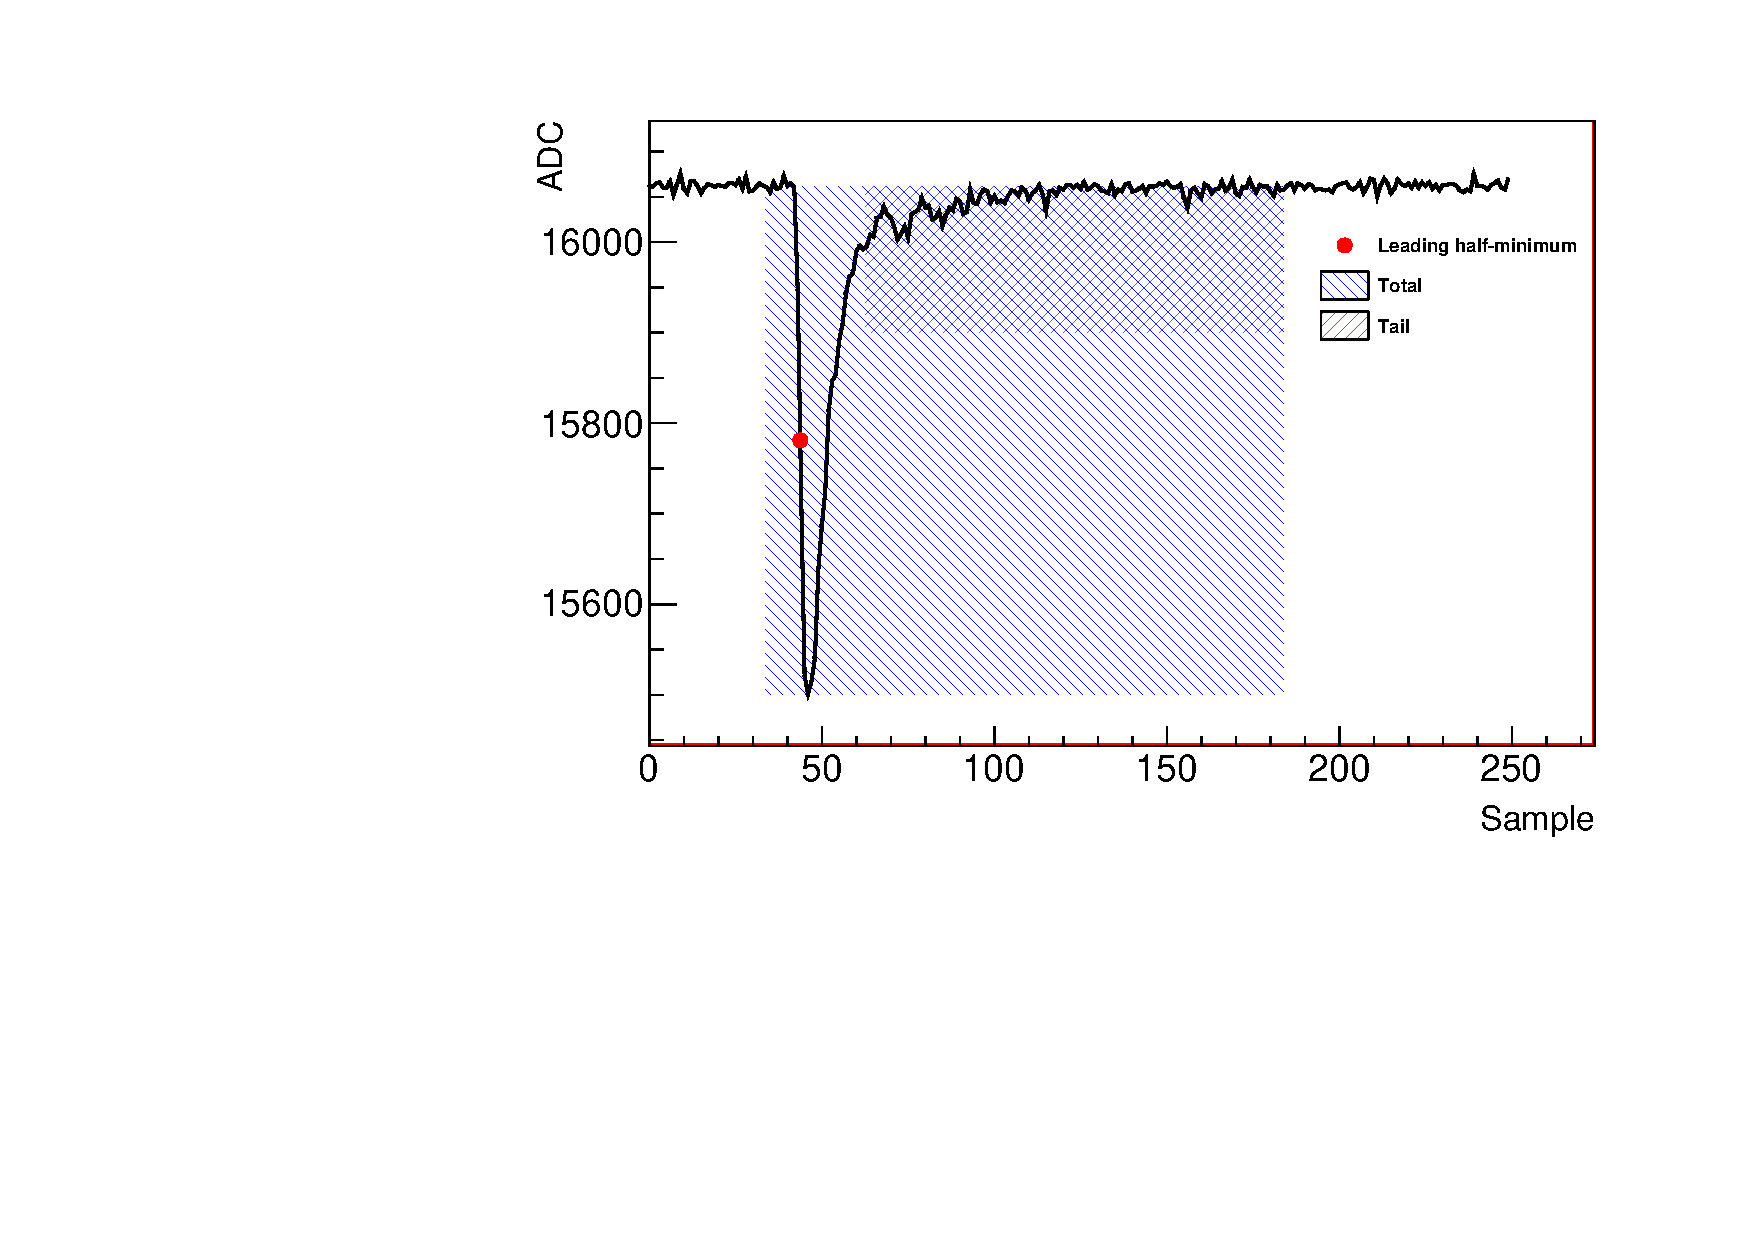
\includegraphics[width=0.6\linewidth]{tex/6-ac227-images/BNL/Waveform_BNL}
	\caption{A typical waveform for an alpha event in the reference sample. The leading half-minimum (circle, red) determines the windows for total pulse area (blue) and tail area (magenta).}
	\label{fig:waveformbnl}
\end{figure}

The \Ac coincident alpha events, labeled RnPo events for the remainder of this document, were found by applying a set of timing, energy, and PSD cuts along with an accidental background subtraction.
Po events were found first by applying the energy and PSD cuts listed in Table~\ref{tab:MatCuts}. 
Rn coincidental events were found by looking in a 12.85 ms time window before a given Po event and applying the same energy and PSD cuts.
This time window was 5 times the lifetime of Po, 2.57 ms, allowing for the collection of nearly all coincident events.
Accidental events were found by looking in the same length time window, using the same energy and PSD cuts, but offset 10 Po lifetimes before a given Po event.
RnPo events were then measured by subtracting the accidental events from the coincident events.
See Figure~\ref{fig:rnpoenpsd} for an example of typical energy and PSD distributions in the reference sample.
\begin{table}[H]
	\centering
	\begin{tabular}{c|c}
		\hline 
		Energy & 0.01 $<$ E $<$ 0.055 nC \\ 
		\hline 
		PSD & 0.31 $<$ PSD $<$ 1.0  \\ 
		\hline 
		$\Delta$t = t$_{\mathrm{delay}}$ - t$_{\mathrm{prompt}}$ & $\Delta$t $<$ 5$\tau_{\textrm{Po}}$ \\ 
		\hline 
	\end{tabular} 
	\caption{Energy, PSD, and time cuts used to find RnPo events where $\tau_{\textrm{Po}}=2.57~\textrm{ms}$. Energy and PSD cuts are applied to both prompt and delay events.}
	\label{tab:MatCuts}
\end{table}

\begin{figure}[!t]
	\centering
	\begin{subfigure}{0.5\linewidth}
		\centering
		\includegraphics[width=1.\linewidth]{"tex/6-ac227-images/BNL/RnPoEn_TimeBin23_S2"}
		\caption{}
	\end{subfigure}%
	\begin{subfigure}{0.5\linewidth}
		\centering
		\includegraphics[width=1.\linewidth]{"tex/6-ac227-images/BNL/RnPoPSD_TimeBin23_S2"}
		\caption{}
	\end{subfigure}
	\caption{Typical energy (a) and PSD (b) distributions for 3.4 livetime-hours of RnPo events in the reference sample after accidental background subtraction.}
	\label{fig:rnpoenpsd}
\end{figure}

The rate of RnPo events was then determined by fitting the RnPo $\Delta t$ distribution with
\begin{equation}
	f(t) = N_0e^{-t/\tau},
	\label{eq:MatDtFit}
\end{equation}
where $N_0$ and $\tau$, the lifetime of \Po (accepted value is 2.569$\pm$0.007 ms), are allowed to vary. 
Using the fit results, the rate was then defined as
\begin{equation}
	R = \frac{N_0 \tau}{\textrm{bin-width}\times\textrm{livetime}},
\end{equation}
\begin{equation}
	\sigma_R = R \times \sqrt{  \left(\frac{\sigma_{N_0}}{N_0}\right)^2 + \left(\frac{\sigma_{\tau}}{\tau}\right)^2 + \frac{2\sigma_{N_{0}\tau}}{N_0\tau} },
\end{equation}
where the livetime was measured, for each run, as the time from the beginning of the run to the last Po event. 
An example of a typical RnPo $\Delta t$ distribution can be seen in Figure~\ref{fig:rnpodttimebin23s2}, where fitting $\Delta t$ with Equation~\ref{eq:MatDtFit} resulted in a \Po lifetime of 2.58$\pm$0.02 ms that agrees well with the accepted value of 2.569$\pm$0.007 ms. It should be noted here that the energy and PSD cuts were made wide enough so that no efficiency correction needed to be applied.

\begin{figure}[H]
	\centering
	\includegraphics[width=1.\linewidth]{"tex/6-ac227-images/BNL/RnPoDt_TimeBin23_S2"}
	\caption{A typical example of the RnPo $\Delta t$ distributions for the 3.4 livetime-hours of events in the reference sample. Left: coincidental and accidental distributions found using the defined energy and PSD cuts. Right: the $\Delta t$ distribution after subtraction of the accidental distribution, fit with Equation~\ref{eq:MatDtFit}.}
	\label{fig:rnpodttimebin23s2}
\end{figure}

\subsection{Results}

The RnPo rate was calculated for each material sample and the reference sample over a period of about six months. These results can be seen in Figure~\ref{fig:ratevstimeallsamples}.
Though statistical errors vary from around 0.6-1\%, overall rates fluctuate by as much as $\pm8\%$ about the mean, indicating the size of unaccounted for systematic errors.

\begin{figure}[!b]
	\centering
	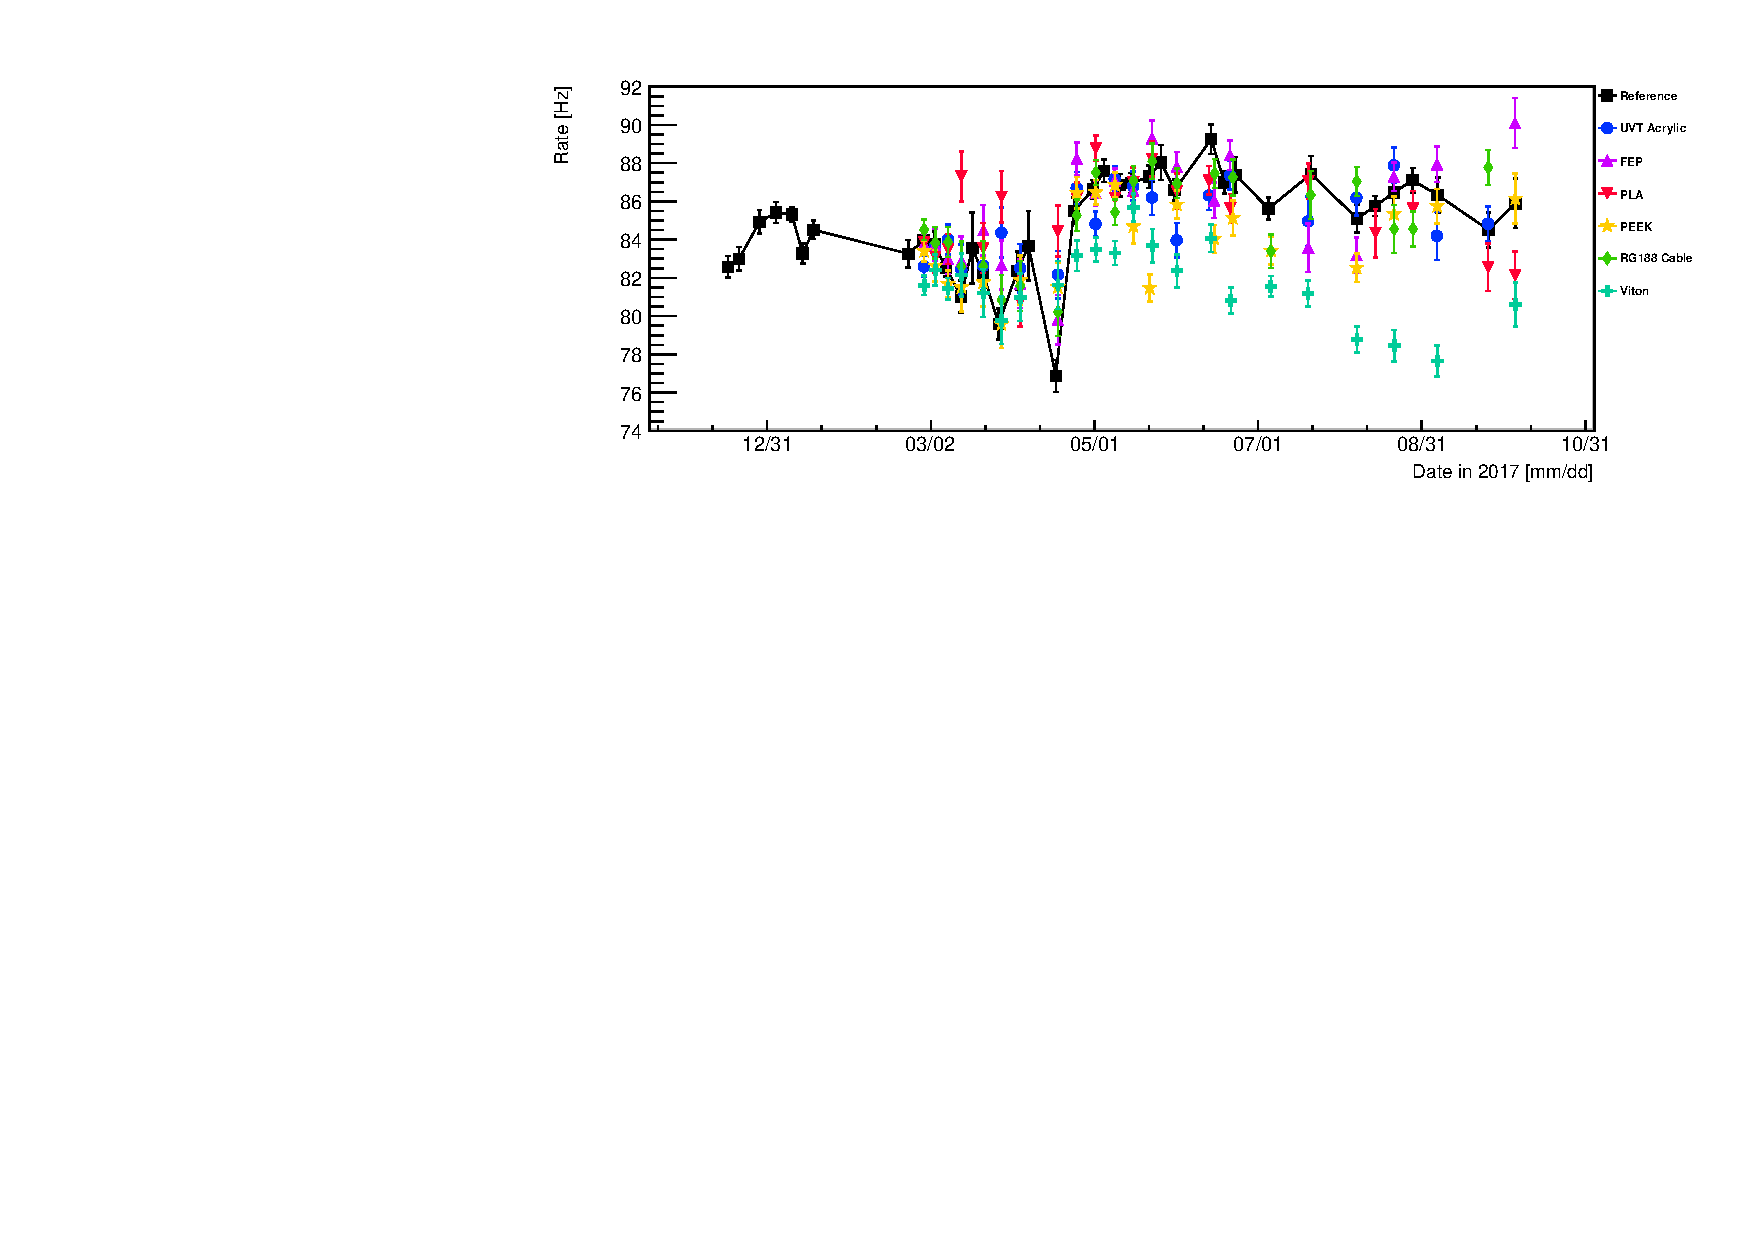
\includegraphics[width=1\linewidth]{tex/6-ac227-images/BNL/RateVsTime_AllSamples}
	\caption{\Ac rate for each material sample. Errors are statistical.}
	\label{fig:ratevstimeallsamples}
\end{figure}

Systematic variations can be better understood by looking at the behavior of the \Po energy distribution through time.
This was done by fitting this distribution for the reference sample with a sum of two Gaussians to account for the non-Gaussian nature of the peak as demonstrated in Figure~\ref{fig:poenfittimebin23s2}.
The mean and 1$\sigma$ width of each of these Gaussians versus time is shown in Figures~\ref{fig:poenmeanvstimes2} and ~\ref{fig:poenwidthvstimes2}.
It can be seen that the \Po energy mean varies about 5\% and the width around 15\%.

\begin{figure}[h]
	\centering
	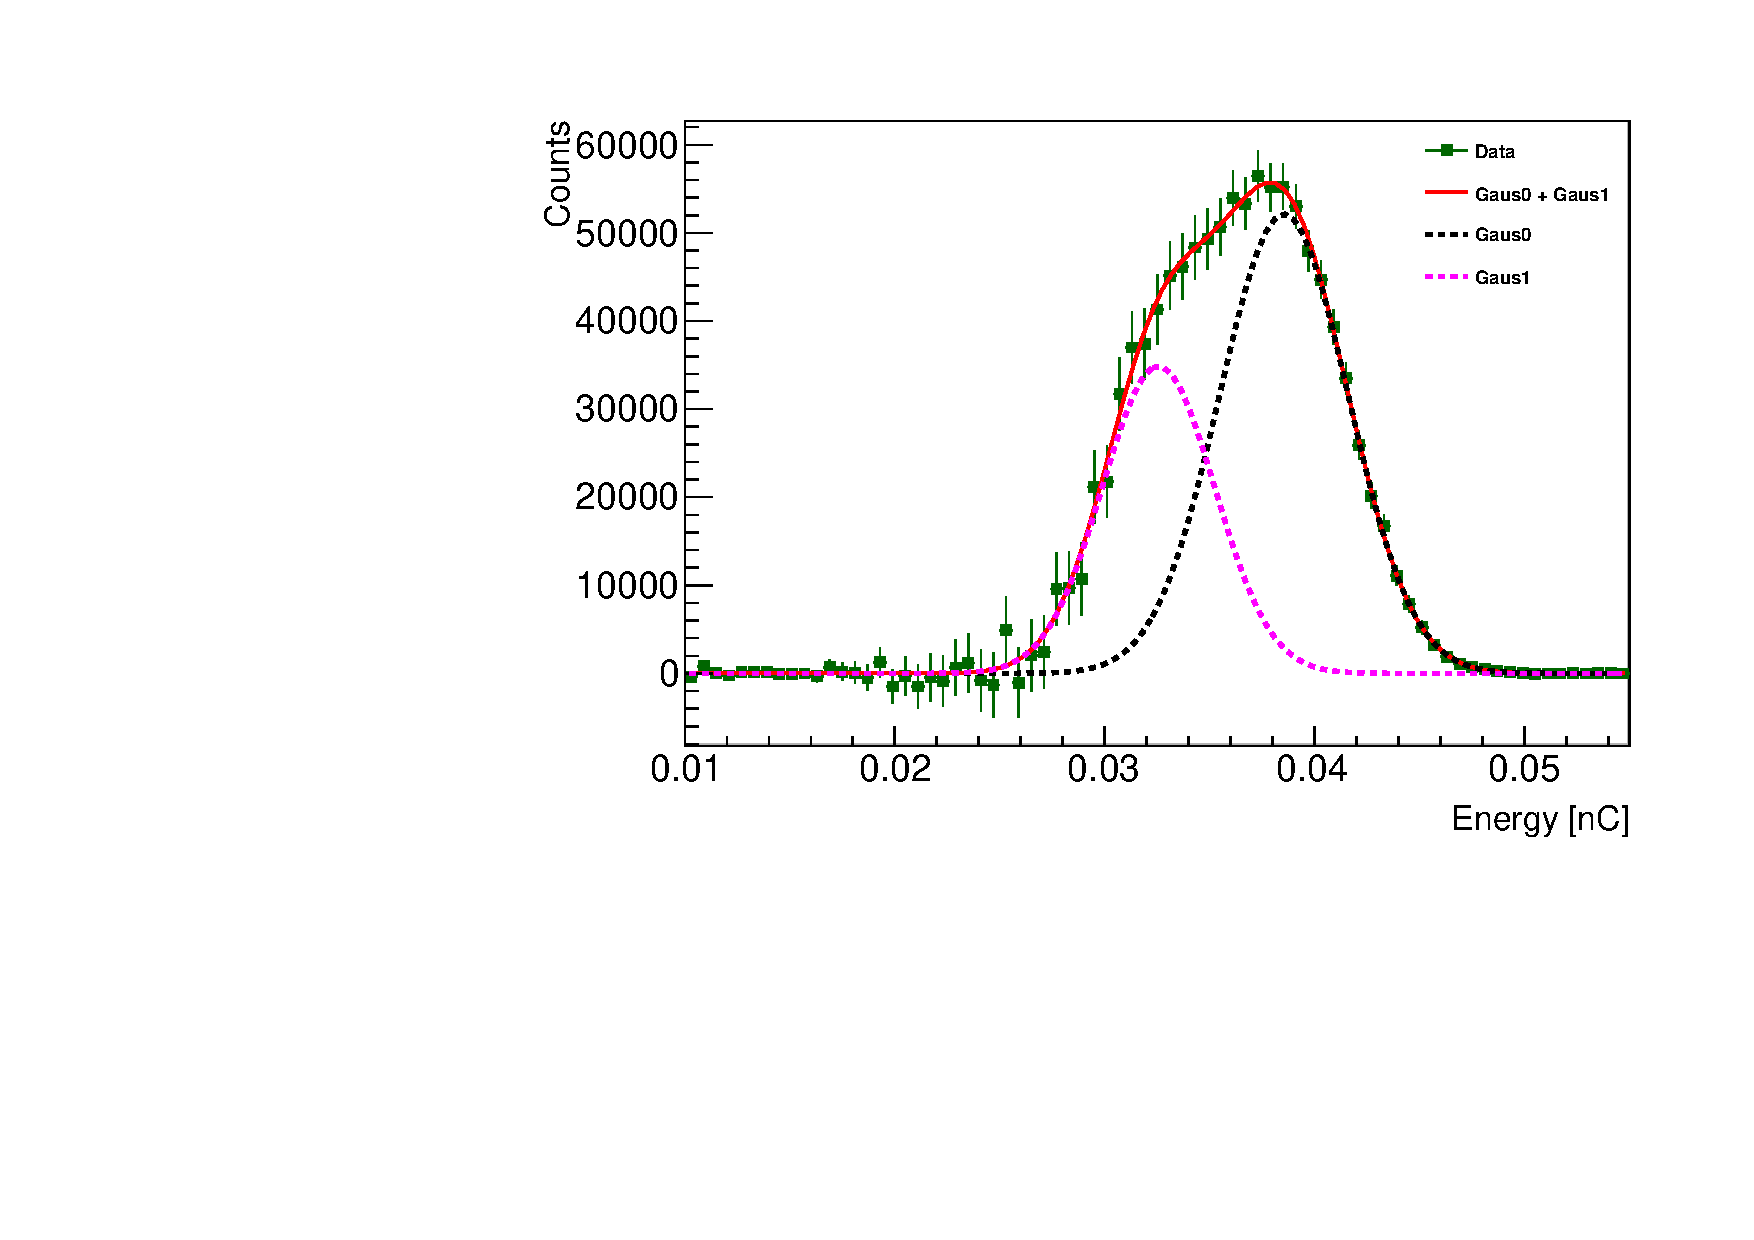
\includegraphics[width=0.6\linewidth]{tex/6-ac227-images/BNL/PoEnFit_TimeBin23_S2}
	\caption{\Po energy distribution for the reference sample, fit with a sum of two Gaussians. The total fit is seen in red, while the two Gaussians are drawn as the pink and black dashed lines.}
	\label{fig:poenfittimebin23s2}
\end{figure}

\begin{figure}[H]
	\centering
	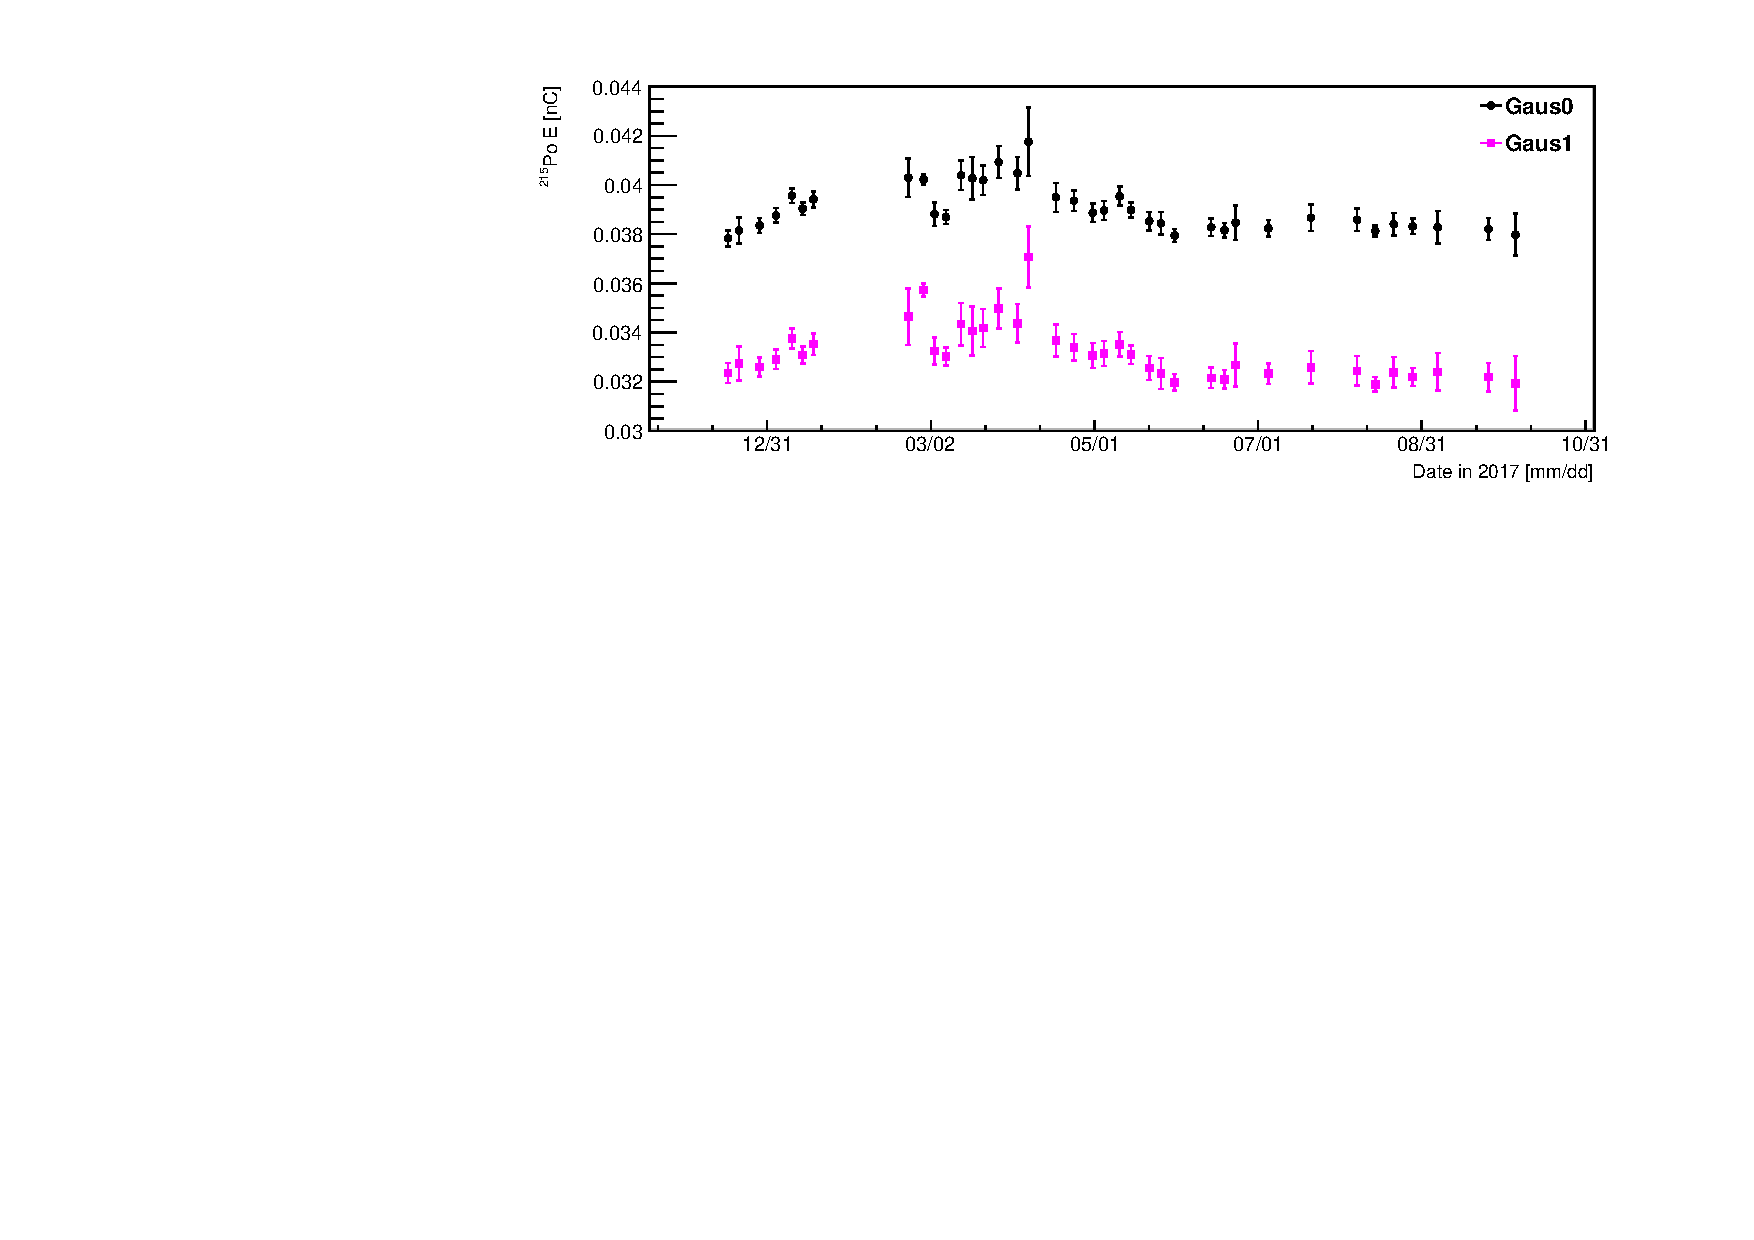
\includegraphics[width=0.9\linewidth]{tex/6-ac227-images/BNL/PoEnMeanVsTime_S2}
	\caption{The mean of the two Gaussians fit to the \Po energy distribution for the reference sample.}
	\label{fig:poenmeanvstimes2}
\end{figure}

\begin{figure}[h]
	\centering
	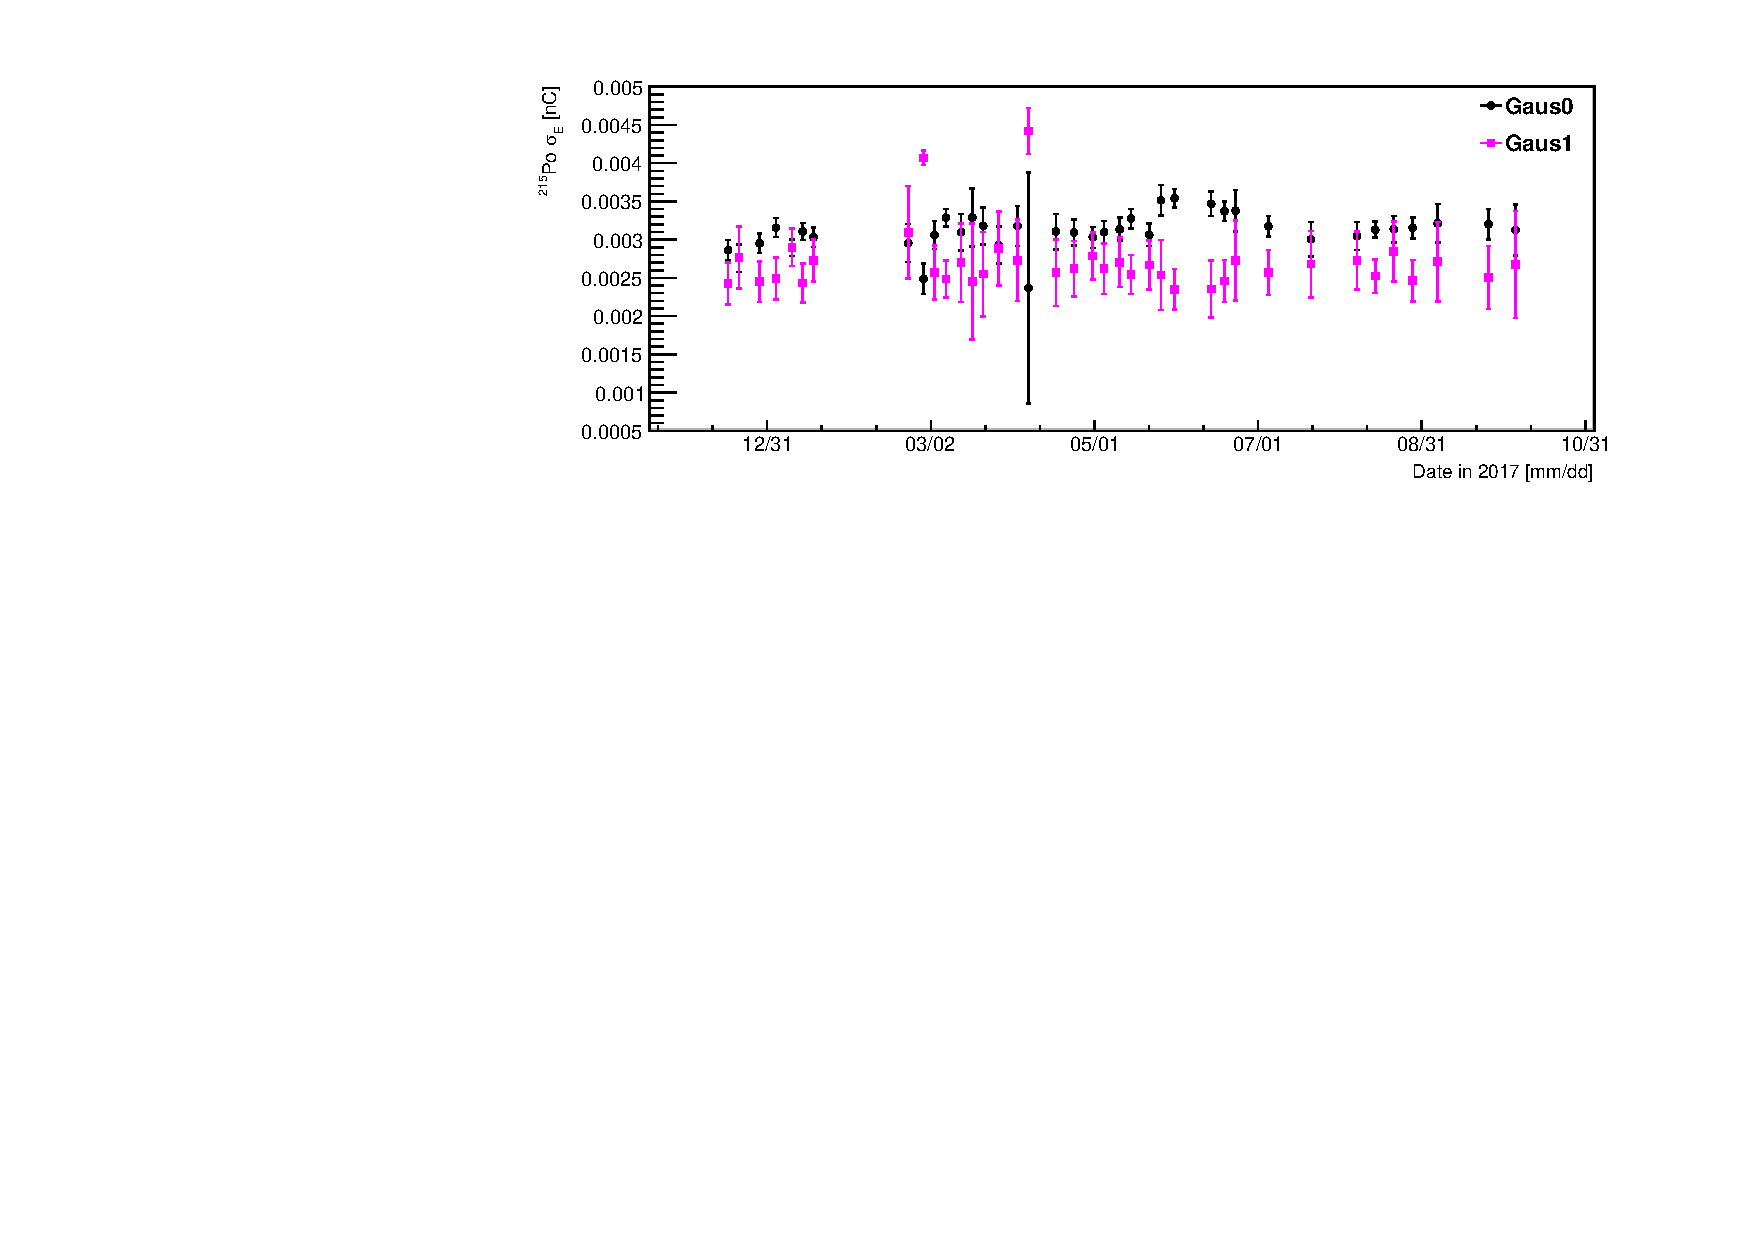
\includegraphics[width=0.9\linewidth]{tex/6-ac227-images/BNL/PoEnWidthVsTime_S2}
	\caption{The 1 $\sigma$ width of the two Gaussians fit to the \Po energy distributions for the reference sample.}
	\label{fig:poenwidthvstimes2}
\end{figure}

The amount of variation seen in measured rates and the \Po energy distribution indicates that the system was not repeatable and, as such, implies significant systematic errors that have not been accounted for. 
The sample vials were repeatedly removed and replaced, possibly shifting the placement of the acrylic holder and the optical grease which coupled the acrylic to the PMT. 
This could possibly account for day-to-day variations, though large changes over time are not understood. 

To account for these variations all material sample rates, $R_M$, were compared to the reference sample rate, $R_{ref}$.
The ratio of the rates was calculated for each time bin as
\begin{equation}
ratio = \frac{R_M}{R_{ref.}},
\end{equation}
\begin{equation}
\sigma_{ratio} = ratio \times \sqrt{\left(\frac{\sigma_{M}}{R_{M}}\right)^2+\left(\frac{\sigma_{ref.}}{R_{ref.}}\right)^2},
\end{equation}
and the results are shown in Figure~\ref{fig:relratevstimeallsamples}.
The ratio of rates versus time, for each material, was fit with a constant and a straight line, the results of which are tabulated in Tables~\ref{tab:MatFitC} and \ref{tab:MatFitLine} respectively.

Except for the case of viton (discussed in the next section) there is no clear decrease in rate observed over the six month period for any material.
Though the chi-squared results for the constant fits are not ideal, the fits to a first degree polynomial do not result in statistically significant decreases with time.
Variations in rate suggest large systematics that have not been accounted for, which imply that these results cannot be trusted to within $\sim \pm$10\%.
Though this may be true, the setup of the experiment, which included a large ratio of material surface area to LiLS area (greater than was true for the AD) and a much higher amount of \Ac activity than would be added to the PROSPECT AD, would be expected to be significantly more sensitive to adsorption.
As such, we could look for general trends that would indicate adsorption.
Since no obvious decreasing trends were observed and visual inspection of the vials determined that the scintillator had not degraded (yellowed) it was concluded that \Ac was not adsorbing onto materials and next steps were taken to include the source in the final detector.

\begin{figure}[H]
	\centering
	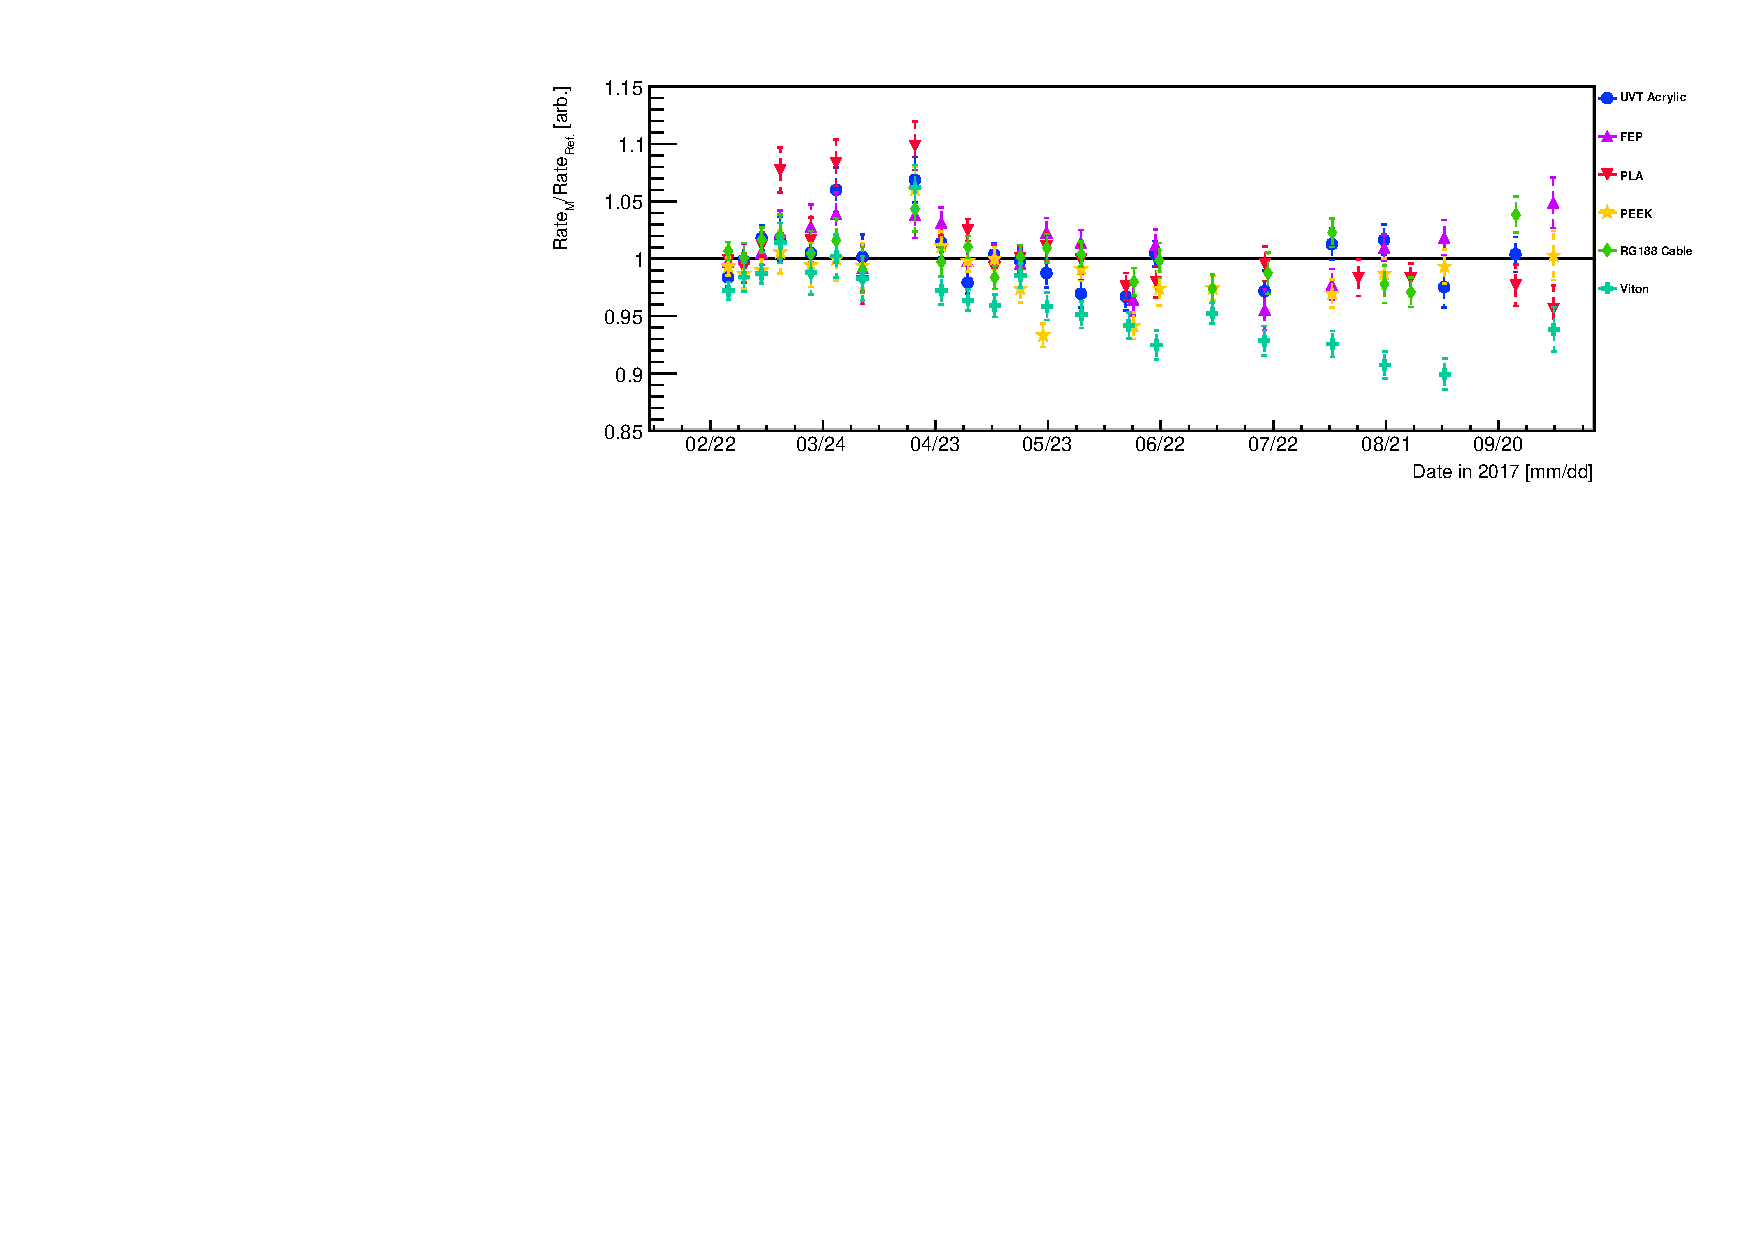
\includegraphics[width=1\linewidth]{tex/6-ac227-images/BNL/RelRateVsTime_AllSamples}
	\caption{\Ac rate for each material sample, $M$, relative to the reference sample.}
	\label{fig:relratevstimeallsamples}
\end{figure}

\begin{table}[H]
	\centering
\begin{tabular}{|c|c|c|}
	\hline 
	\textbf{Material} & \textbf{Constant} & \textbf{$\chi^2$/NDF} \\ 
	\hline 
	UVT Acrylic  & 0.997 $\pm$ 0.003 & 56.5/20 = 2.82 \\ 
	\hline 
	FEP & 1.005 $\pm$ 0.003 & 44.1/20 = 2.21 \\ 
	\hline 
	PLA & 1.003 $\pm$ 0.003 & 80.6/20 = 4.03 \\ 
	\hline 
	PEEK & 0.985 $\pm$ 0.003 & 70.9/20 = 3.55 \\ 
	\hline 
	RG188 Cable & 1.001 $\pm$ 0.003 & 38.3/21 = 1.82 \\ 
	\hline 
	Viton  & 0.960 $\pm$ 0.002 & 136.3/21 = 6.49 \\ 
	\hline 
\end{tabular} 
\caption{The results of fitting the relative rate for each material sample with a constant.}
\label{tab:MatFitC}
\end{table}

\begin{table}[H]
	\centering
\begin{tabular}{|c|c|c|c|}
	\hline 
	\textbf{Material} & \textbf{Constant} & \textbf{Slope [ratio/yr]} & \textbf{$\chi^2/NDF$} \\ 
	\hline 
	UVT Acrylic  & 1.5 $\pm$ 0.8 & -0.01 $\pm$ 0.02 & 56.2/19 = 2.96 \\ 
	\hline 
	FEP  & 1.3 $\pm$ 0.8 & -0.005 $\pm$ 0.018 & 44.0/19 = 2.32 \\ 
	\hline 
	PLA  & 4.4 $\pm$ 0.8 & -0.07 $\pm$ 0.02 & 64.3/19 = 3.38 \\ 
	\hline 
	PEEK  & 2.9 $\pm$ 0.8 & -0.04 $\pm$ 0.02 & 65.2/19 = 3.43 \\ 
	\hline 
	RG188 Cable  & 2.3 $\pm$ 0.8 & -0.03 $\pm$ 0.02 & 35.7/20 = 1.79\\ 
	\hline 
	Viton  & 7.7 $\pm$ 0.7 & -0.14 $\pm$ 0.02 & 48.9/20 = 2.45 \\ 
	\hline 
\end{tabular} 
\caption{The results of fitting the relative rate for each material with a straight line.}
\label{tab:MatFitLine}
\end{table}

\subsubsection{Viton}

Observation of the rate of \Ac in the viton o-ring material sample vial initially indicated a decrease in rate over time, about 10\% compared to the reference vial over a six month period.
Upon further inspection, though, it became clear that the energy spectrum, of the Rn events in particular, shift toward the system threshold as time goes on.
This caused a loss of events, not due to adsorbance, but rather due to threshold effects.

Figure~\ref{fig:rnpoenfirstandlast} shows the \Rn and \Po energy distributions in the first and last time bins for both viton and PEEK.
It can be seen that at the last time bin the viton distributions sit against the threshold, compared to the PEEK distributions which approach but do not get close to the threshold.
To quantify this the \Rn spectrum was fit with a sum of two Gaussians and the widths versus time are shown in Figure~\ref{fig:rnenwidths8}.
It can be seen that the lower energy Gaussian becomes narrower as time goes on, indicating a loss of events due to threshold effects.
Therefore, it was concluded that the decrease in \Ac rate observed in the viton o-ring sample was due to threshold effects rather than adsorption.


\begin{figure}[H]
	\begin{subfigure}{1\linewidth}
	\centering
	\includegraphics[width=1.\linewidth]{"tex/6-ac227-images/BNL/RnPoEn_FirstAndLast_S8"}
	%\caption{}
	\label{fig:rnpoenfirstandlasts8}
\end{subfigure}
\begin{subfigure}{1\linewidth}
	\centering
	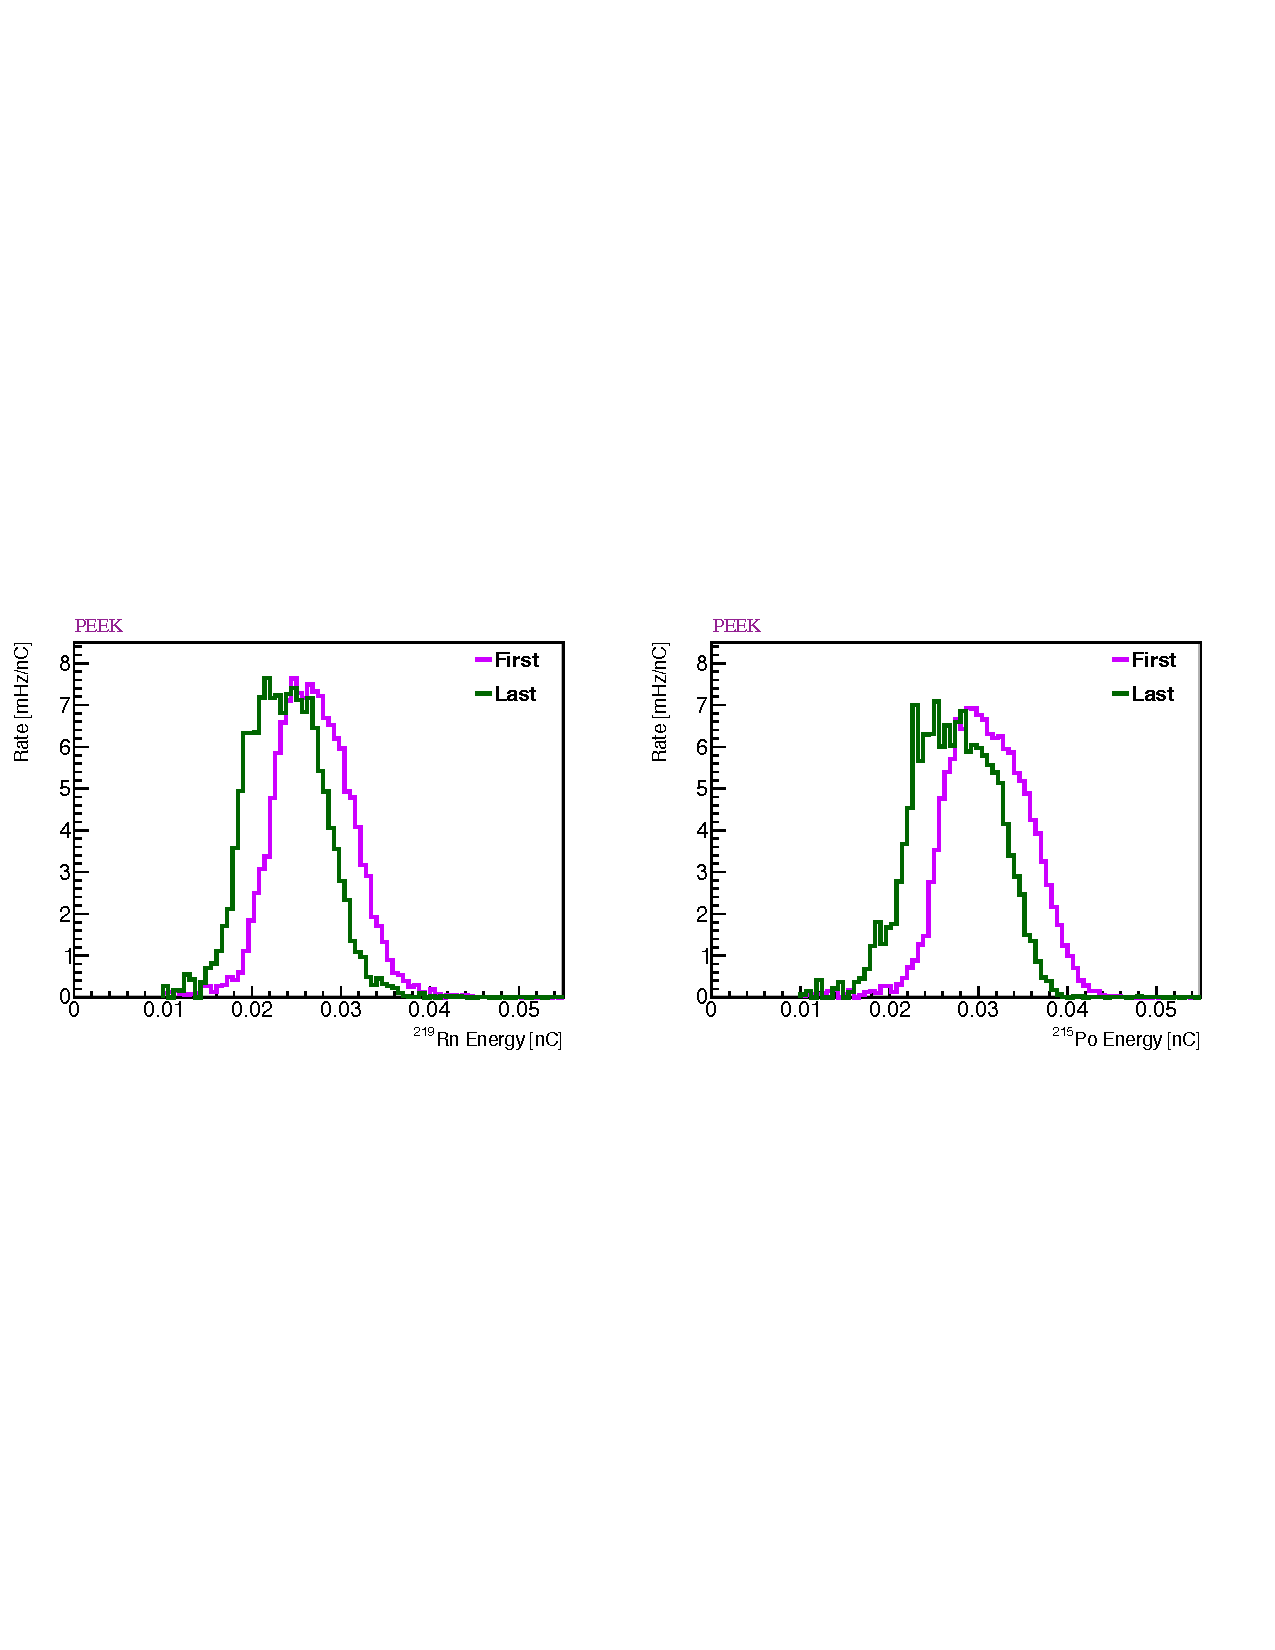
\includegraphics[width=1\linewidth]{tex/6-ac227-images/BNL/RnPoEn_FirstAndLast_S6}
	%\caption{}
	\label{fig:rnpoenfirstandlasts6}
\end{subfigure}
\caption{\Rn and \Po energy spectra for both the viton o-ring (top) and PEEK (bottom) material samples during the first and last time bins.}
\label{fig:rnpoenfirstandlast}
\end{figure}

\begin{figure}[H]
	\centering
	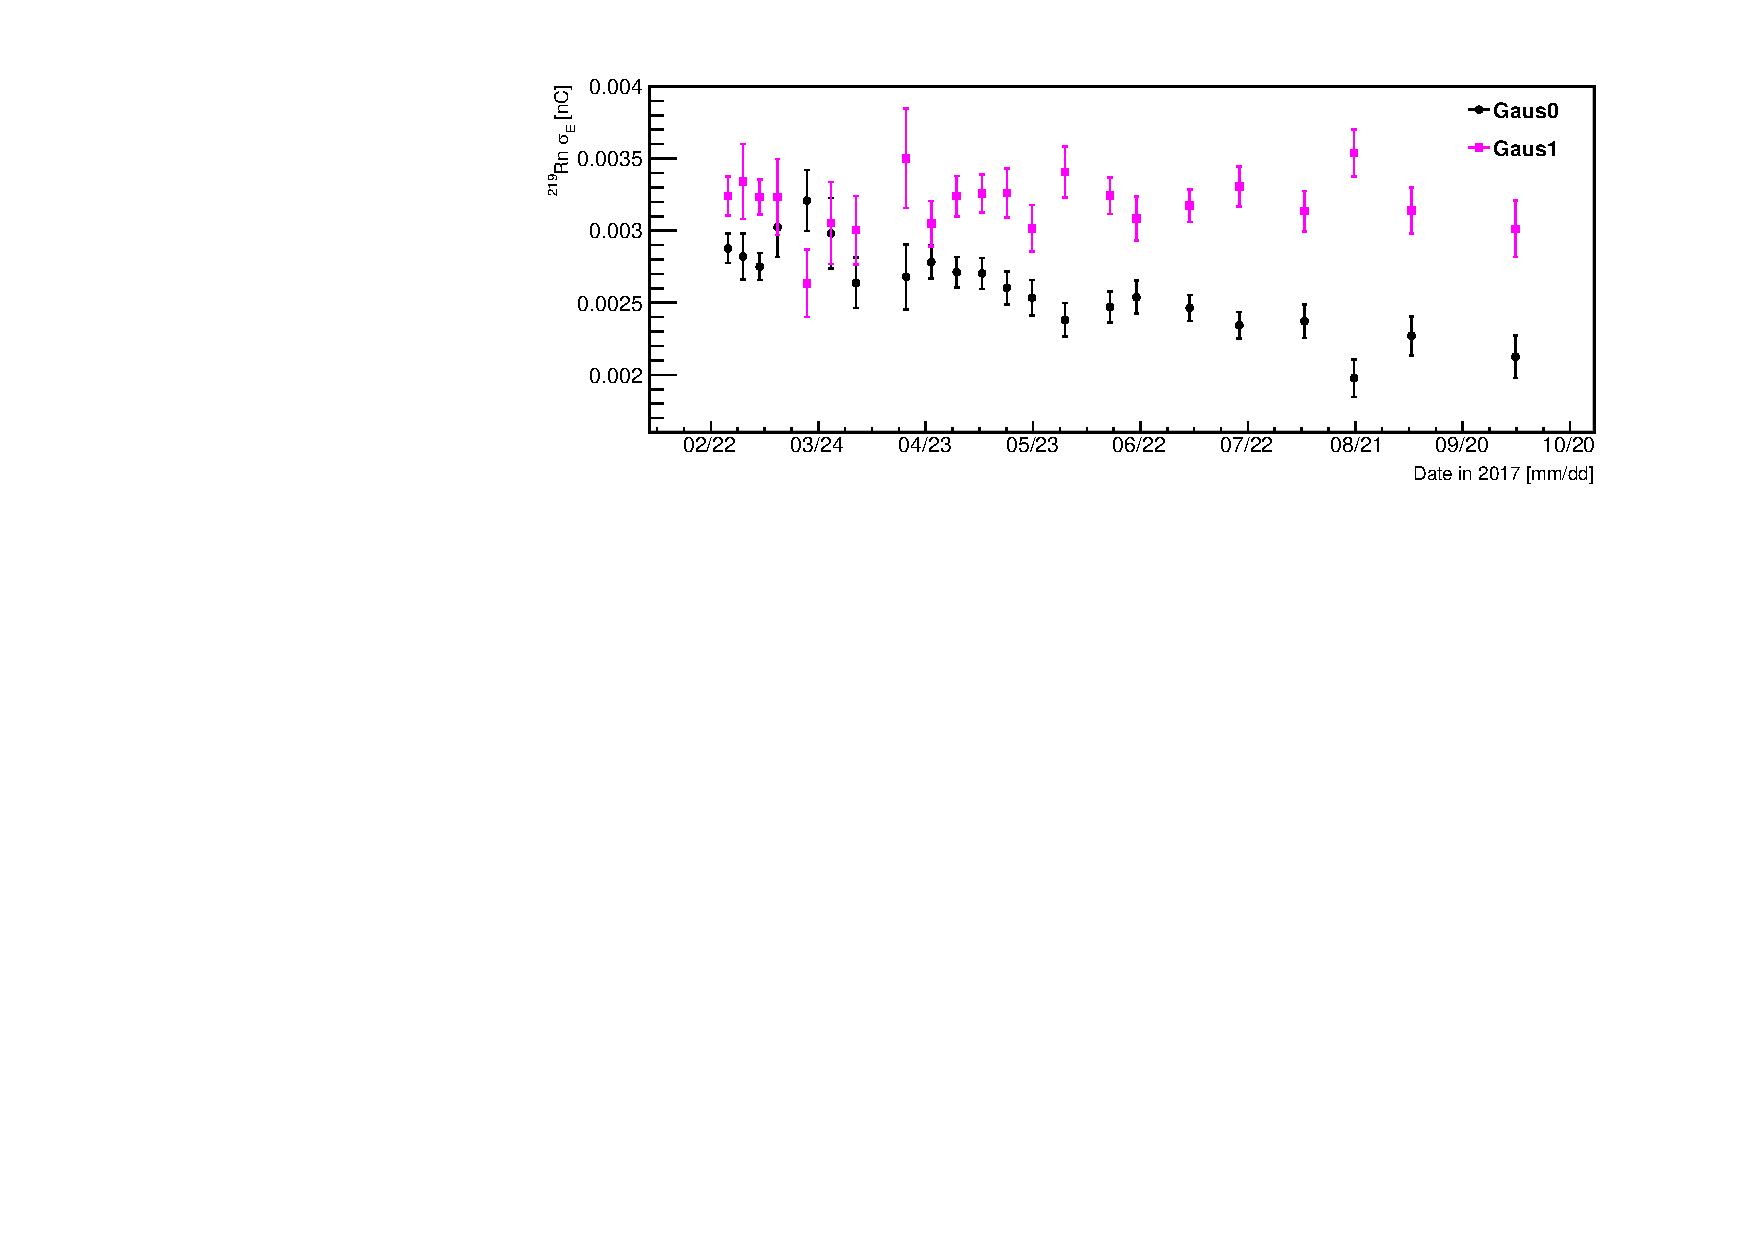
\includegraphics[width=0.9\linewidth]{tex/6-ac227-images/BNL/RnEnWidth_S8}
	\caption{The 1$\sigma$ width of two Gaussians fit to the \Rn energy spectrum versus time for the viton o-ring material sample. Black (circle): higher energy Gaussian, Magenta (square): lower energy Gaussian.}
	\label{fig:rnenwidths8}
\end{figure}



\section{\Ac in the PROSPECT AD}

Material compatibility testing determined that \Ac did not significantly adsorb onto detector materials, confirming that it could be used as a uniformly distributed source.
It will be noted here that \Ac spiked LiLS was added to a prototype detector that consisted of two stacked segments \cite{Ashenfelter:2018cli}.
This was done to determine that the \Ac did not degrade the performance of the liquid scintillator and that it did not introduce significant background.
Initial results from the prototype concluded that it did neither and provided the last step of evidence needed before addition to the full-scale detector.

\subsection{Spiking the LiLS}

After concluding that \Ac would be added to the AD, the goal was to obtain a final activity of 0.01 Bq/segment. 
Assuming a total LiLS mass of 4600 kg and an active mass of 3939 kg implies a total \Ac activity of 1.8 Bq.
The stock solution from which the LiLS was spiked was the same stock that was used for the material studies, which had an activity of $\sim$9.13 Bq/g on December 13, 2017, the day the spiking procedure was performed.
This means that $\sim$200 mg of the stock was needed to spike the LiLS.

In order to add \Ac to the total detector, a vial of spiked LiLS was added to a 55-gallon drum of LiLS prepared previously for detector filling.
Before the detector was filled all drums were added to an ISO-tank (a tank container which is built to the International Organization for Standardization standards) and bubbled with nitrogen to ensure thorough mixing of the LiLS from all drums and the \Ac.

We spiked the drum by diluting the concentration of the stock solution by adding it to an intermediate vial of production LiLS before spiking the vial that was added to the drum. 
This was done to reduce the relative uncertainty from the $\pm10$ mg uncertainty of the balance used to weigh the vials and allowed an assessment of the activity of the remaining vial.
The procedure was duplicated in a second set of vials so that the first vial could immediately be added to the LiLS drum and the second set could be used to measure the final activity and deduce that of the emptied one.

The spiking procedure was performed using four vials, V0, V1, V2, and V3.
The steps were:
\begin{enumerate}
	\item Fill all four vials with production LiLS
	\item Fill V1 and V2 with the \Ac spiked LiLS stock solution
	\item Fill V0 with solution from V1 until desired activity is reached
	\item Fill V3 with solution from V2 until desired activity is reached
	\item Empty V0 into drum of production LiLS 
\end{enumerate}
See Figure~\ref{fig:spikingprocedure} for a graphic of these steps along with Table~\ref{tab:SpikeProc} for a list of the weights of all solutions added and removed from the vials.
\begin{figure}[!b]
	\centering
	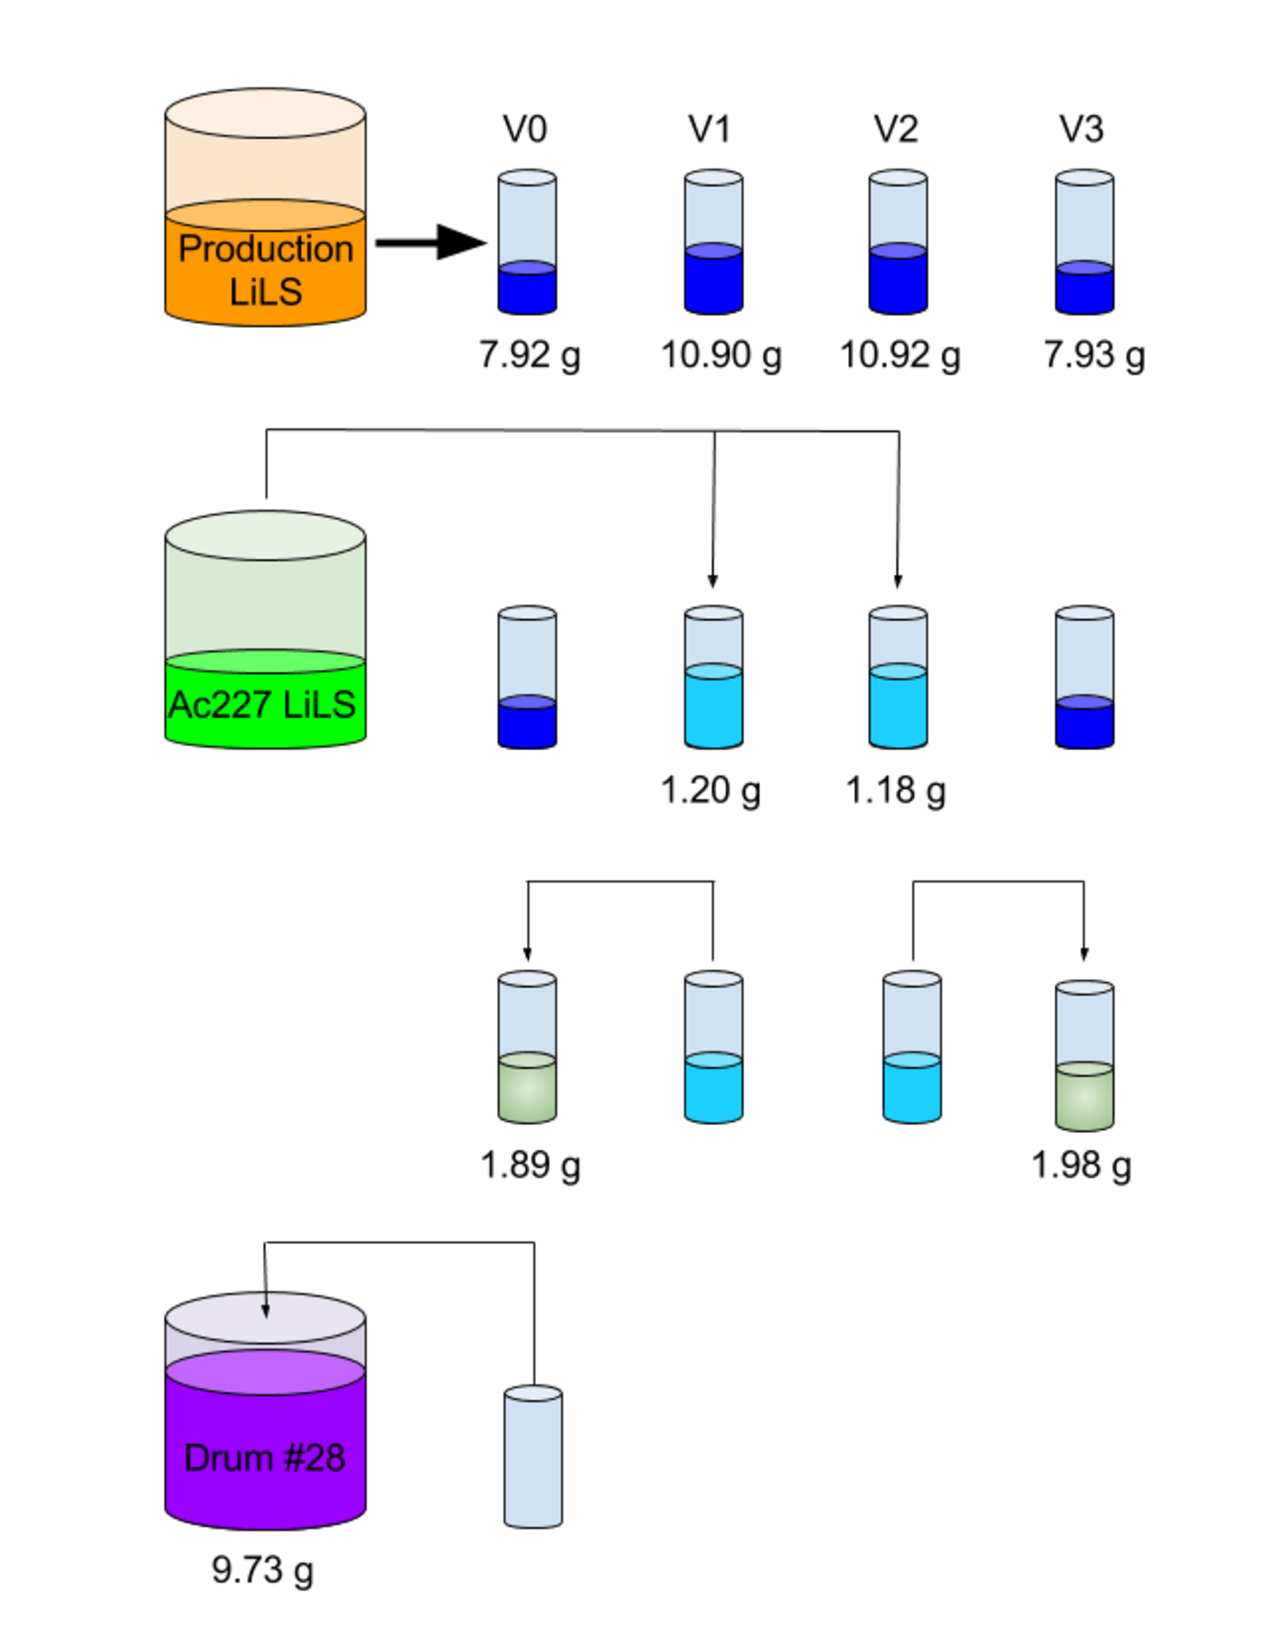
\includegraphics[width=0.5\linewidth]{tex/6-ac227-images/BNL/SpikingProcedure}
	\caption{A graphic of the procedure used to spike the drum of LiLS with \Ac for filling of the AD. The numbers indicate the amount of LiLS transfered, rather than the total weight.}
	\label{fig:spikingprocedure}
\end{figure}
The amount of LiLS that was transfered at each step was initially calculated so that $\sim$10 g would remain in all vials at the end.
The vials were filled and the transfers were completed using pipettes, therefore, some drops inevitably remained in the pipette at every step.
Vials V1 and V2 were gently swirled after the addition of the \Ac spiked LiLS in an attempt to mix the solution.

\begin{table}[!t]
	\centering
\begin{tabular}{r|c|c|c|c}
	\hline 
	& \textbf{V0} & \textbf{V1} & \textbf{V2} & \textbf{V3} \\ 
	\hline 
	\textbf{Production LiLS added, $m_1$ (g)}  & 7.92 & 10.90 & 10.92 & 7.925 \\ 
	\hline 
	\textbf{\Ac spiked solution added, $m_2$ (g)} &  & 1.20 & 1.18 &  \\ 
	\hline 
	\textbf{Solution removed, $m_3$ (g)} &  & 2.047 & 2.09 &  \\ 
	\hline 
	\textbf{Solution added, $m_4$ (g)} & 1.885 &  &  & 1.98 \\ 
	\hline 
\end{tabular} 
\caption{The weight of all solutions added and removed from the four vials for spiking of the LiLS with \Ac for filling of the AD.}
\label{tab:SpikeProc}
\end{table}

The expected \Ac rate, $A$, in vials V0(V3) was calculated as
\begin{equation}
	A = C~m_2 \frac{m_4}{m_1 + m_2},
\end{equation}
where $C$ is the activity of the \Ac spiked stock solution, 9.13 Bq/g, $m_1$ is the amount of production LiLS added to V1(V2), $m_2$ is the amount of the stock solution added to V1(V2), and $m_4$ is the amount of solution from V1(V2) that was added to V0(V3).
The expected rate in vials V1(V2) was then calculated as 
\begin{equation}
A = C~m_2 \left(1 - \frac{m_3}{m_1 + m_2}\right),
\end{equation}
where $m_3$ is the amount of solution removed from V1(V2).
The expected \Ac activity for each vial is listed in Table~\ref{tab:SpikeExpA}.

The \Ac rate in vials V1, V2, and V3 were measured after adding V0 to the drum of LiLS.
The rate of \Ac in V3 should be similar to the rate in AD, recalling that the goal was 1.8 Bq.
A plot of the measured rates for each vial is shown in Figure~\ref{fig:ADVials}.
Each of these rates was fit with a constant, with the results of these fits listed in Table~\ref{tab:SpikeExpA}.
\begin{table}[h]
	\centering
	\begin{tabular}{c|c|c}
		\hline 
		\textbf{Vial} & \textbf{Expected Activity [Bq]} & \textbf{Measured Rate [Hz]} \\ 
		\hline 
		V0 & 1.71 & --- \\ 
		\hline 
		V1 & 9.10 &  9.48 $\pm$ 0.04  \\ 
		\hline 
		V2 & 8.91 & 9.38 $\pm$ 0.06\\ 
		\hline 
		V3 & 1.76 & 0.696 $\pm$ 0.001 \\ 
		\hline 
	\end{tabular} 
	\caption{Expected and measured \Ac activity in vials prepared for spiking the LiLS. }
	\label{tab:SpikeExpA}
\end{table}
It can be seen that the measured rates in V1 and V2 are about 4\% higher than expectation, and the rate in V3 is about 50\% lower.
A possible explanation for this discrepancy is that the solution was not sufficiently mixed before transferring between the stock solution and the vials and between the vials themselves. 
This is bolstered by the fact that the measured rates in V2+V3 = 10.08 Hz, compared to the expected rate of 10.67 Hz, well within a 10\% systematic error that could be assigned from uncertainties in the mixing and measurement procedure.

If this experiment was repeated a more thorough testing of transfer procedures would need to be performed.
In conclusion, the measured rate in V3 indicates that the \Ac rate in the PROSPECT AD should be around 0.7 Hz in the total volume ($\sim0.6 \pm 0.06$ Hz in the active volume), less than half of the initial goal.

\begin{figure}[!t]
	\centering
\begin{subfigure}{1\linewidth}
	\centering
	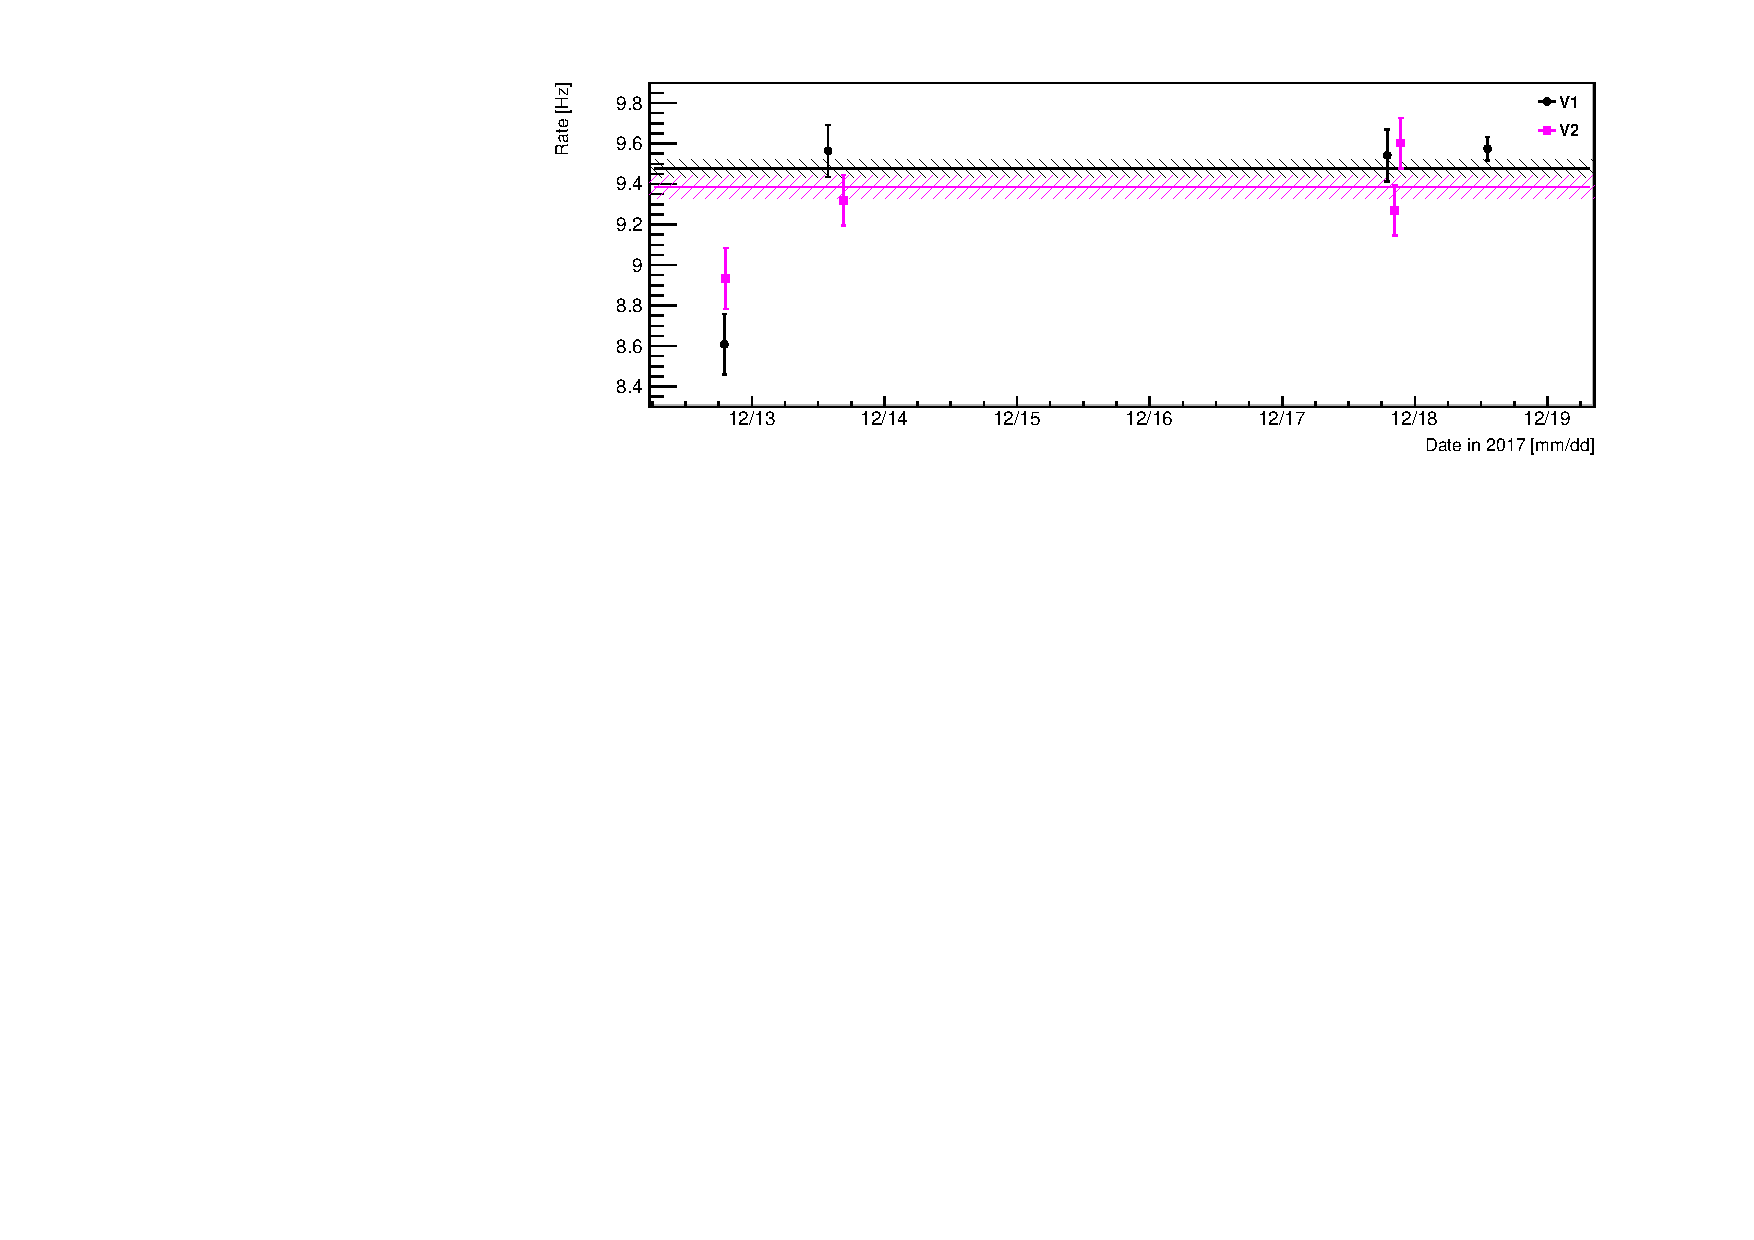
\includegraphics[width=0.9\linewidth]{tex/6-ac227-images/BNL/AD_Rates}
	%\caption{}
	\label{fig:adrates}
\end{subfigure}
\begin{subfigure}{1\linewidth}
	\centering
	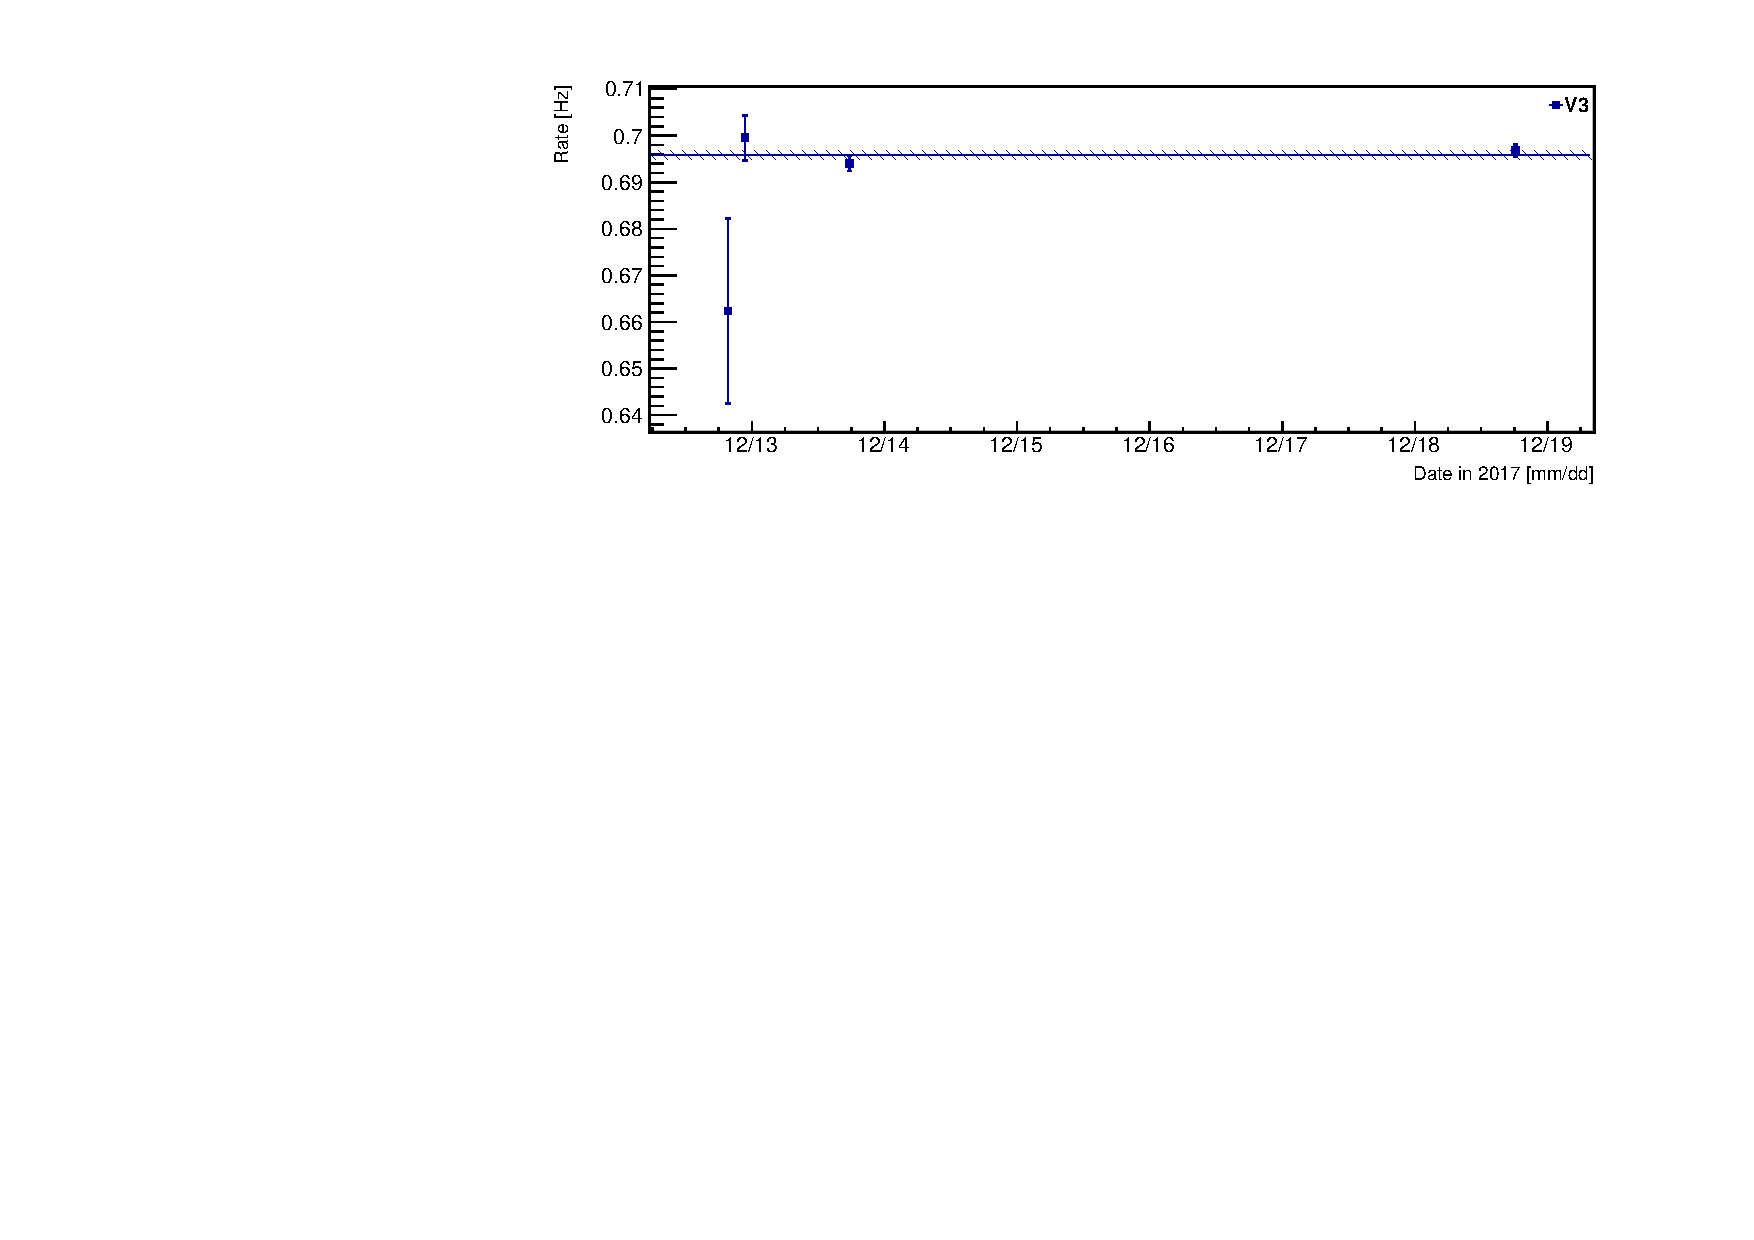
\includegraphics[width=0.9\linewidth]{tex/6-ac227-images/BNL/AD_RateV3}
	%\caption{}
	\label{fig:adratev3}
\end{subfigure}
\caption{Measured \Ac rates of vials used in the procedure performed to add \Ac to the LiLS of the PROSPECT AD. Top: intermediate vials V1 and V2. Bottom: V3, filled in the same method as the vial that was added to the drum of LiLS. All rates were fit with a constant, the results drawn as solid lines with hashed lines representing the error.}
\label{fig:ADVials}
\end{figure}


\subsection{Data Set}

PROSPECT began taking data in March 2018.
The data set used for the \Ac analysis ran from March 5, 2018 - October 6, 2018, with a break from March 31, 2018 - April 17, 2018 when the detector was off for maintenance. 
The total runtime was 4048.9 hrs (2293.7 hrs reactor on, 1755.2 hrs reactor off), which, after dead time corrections, resulted in 4011.7 hrs of livetime data.

During the data collection period used for this analysis, several PMTs exhibited abnormal behavior, including current instabilities, and are no longer in operation.
Preliminary theories for the cause of this are that LiLS leaked into the PMT housings and damaged the voltage dividers, but this has yet to be confirmed. 
To account for this all segments that `turned off' during the data period are excluded in this analysis. 
The result is 90 active segments, as shown in Figure~\ref{fig:segments}. \footnote{Segment 111, though excluded from this analysis, was never off during this data-set. Rather, other abnormalities were observed in this segment that were believed to not be real volume effects. Since this segment is a fiducial segment, and therefore is not included in the oscillation analysis, for simplicity it was excluded in this analysis.}

\begin{figure}[h]
	\centering
	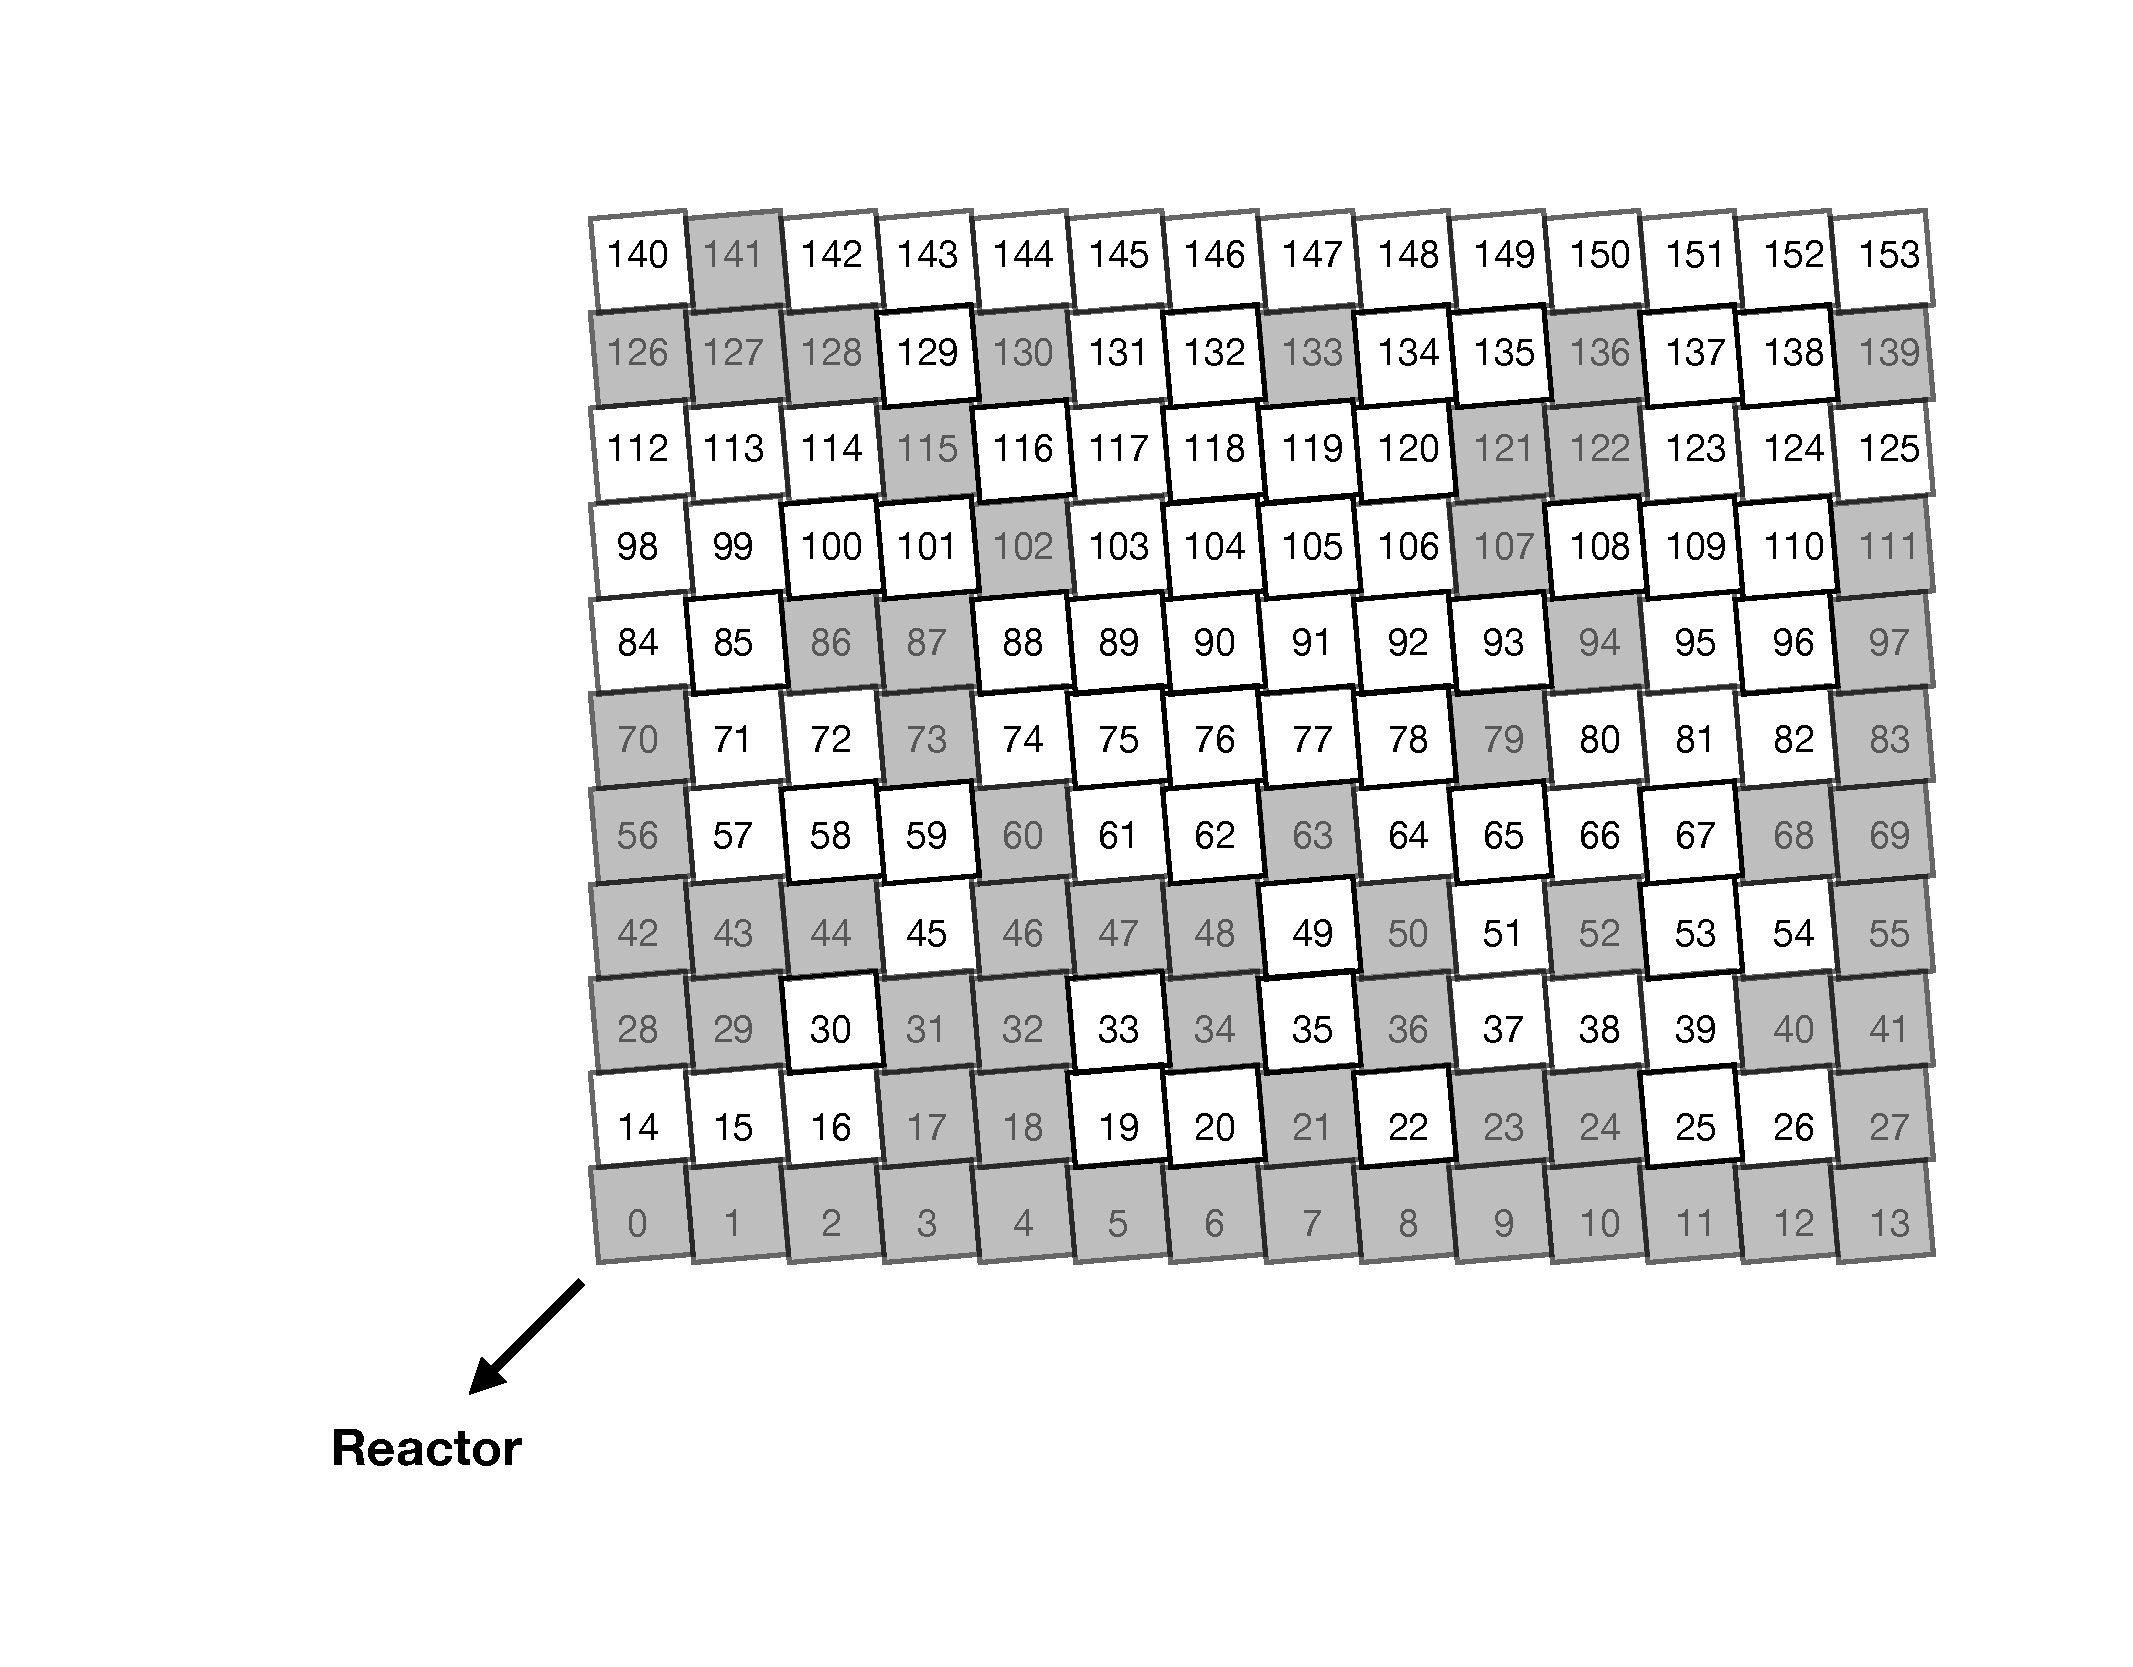
\includegraphics[width=0.7\linewidth]{tex/6-ac227-images/AD_DataSet/Segments}
	\caption{Graphic of 154 segments of the PROSPECT AD. Grayed out segments are those that `turned off' during the data period and are excluded in this analysis.}
	\label{fig:segments}
\end{figure}


\subsection{Event Selection}

RnPo events in the PROSPECT detector were found by looking at event clusters.
A cluster is defined as a collection of events that occur within 20 ns of each other.
Time coincident events were found by first looking for delayed (Po) events. 
These events were required to be in a single multiplicity cluster, because \Po emits a single mono-energetic alpha with no accompanying gammas, and pass broad energy and PSD cuts as outlined in Table~\ref{tab:RnPoCuts}.

We identified coincident prompt events by looking in a 5$\tau$ time window before the delay event, where $\tau = 2.57$ ms is the lifetime of $^{215}$Po.
We required that the highest energy event in a given cluster in that time window occurred in the same segment as the delay event and passed the energy and PSD cuts in Table~\ref{tab:RnPoCuts}.
Due to the close proximity to the neutron capture on $^6$Li signal ($\sim$0.55 MeV), only events where $\Delta t = t_{\textrm{delay}}-t_{\textrm{prompt}} > 0.5$~ms were accepted.
Since the neutron capture time in PROSPECT is about 50 $\mu$s, this cut effectively removes neutron capture contamination in the event selection.
The prompt and delayed alphas are expected to be within a few tens of microns of each other, but, due to detector position resolution, $\Delta z = \abs{z_{\textrm{delay}} - z_{\textrm{prompt}}}$ was required to be less than 250~mm.

Accidental prompt events were found by looking in a 5$\tau$ time window offset 10$\tau$ before the delay event. 
The same cuts applied to coincidental prompt events were applied to accidental prompt events.

\begin{table}[!t]
	\centering
\begin{tabular}{c|c}
	\hline 
	Prompt Energy & 0.48 $<$ E $<$ 1.18 MeV \\ 
	\hline 
	Delay Energy & 0.61 $<$ E $<$ 1.18 MeV \\ 
	\hline 
	PSD & 0.16 $<$ PSD $<$ 0.36 \\ 
	\hline 
	$\Delta z = |z_{\textrm{delay}} - z_{\textrm{prompt}}|$ & $\Delta z < 250$ mm  \\ 
	\hline 
	$\Delta t = t_{\textrm{delay}} - t_{\textrm{prompt}}$ & $0.5 < \Delta t < 5\tau$ ms \\ 
	\hline 
\end{tabular} 
\caption{First pass, broad cuts used to find RnPo events, where $\tau = 2.57~\textrm{ms}$ is the lifetime of \Po. A second pass of the data changes the requirement for the low bounds of energy and PSD to be $< 4 \sigma$ from the mean.}
\label{tab:RnPoCuts}
\end{table}

In addition to energy, PSD, and position cuts a pileup veto was applied to all events.
At the time of a trigger event all boards are signaled to begin a 592 ns acquisition window. 
Events arriving at the end of this window do not re-trigger the data acquisition system, thus causing truncated waveforms.
In order to avoid using these truncated events, any cluster preceded by another cluster in a 800 ns window is vetoed. 

The broad energy and PSD cuts listed in Table~\ref{tab:RnPoCuts} are applied on a first pass analysis of the PROSPECT data.
Changes in detector performance over time, including decreasing energy resolution and PSD, required a second pass of the data, in which the lower bounds of the energy and PSD cuts were changed to be 4$\sigma$ lower than the mean of the distributions for a given time bin or segment.
The range of 4$\sigma$ was chosen in order to avoid large efficiency corrections for these cuts.

To check if these cuts correctly selected RnPo events, one can look at the position distribution of \Po events along $z$, as shown for one segment in Figure~\ref{fig:poposseg76}.
As expected this distribution is fairly stable across the length of the segment and almost all events are reconstructed inside the physical length of the cell (a small percentage are reconstructed in the mineral oil inside the PMT housing).
The PSD versus energy and \Po energy versus \Rn energy distributions, after accidental subtraction, can be seen in Figure~\ref{fig:RnPoPSDEn}.

\begin{figure}[h]
	\centering
	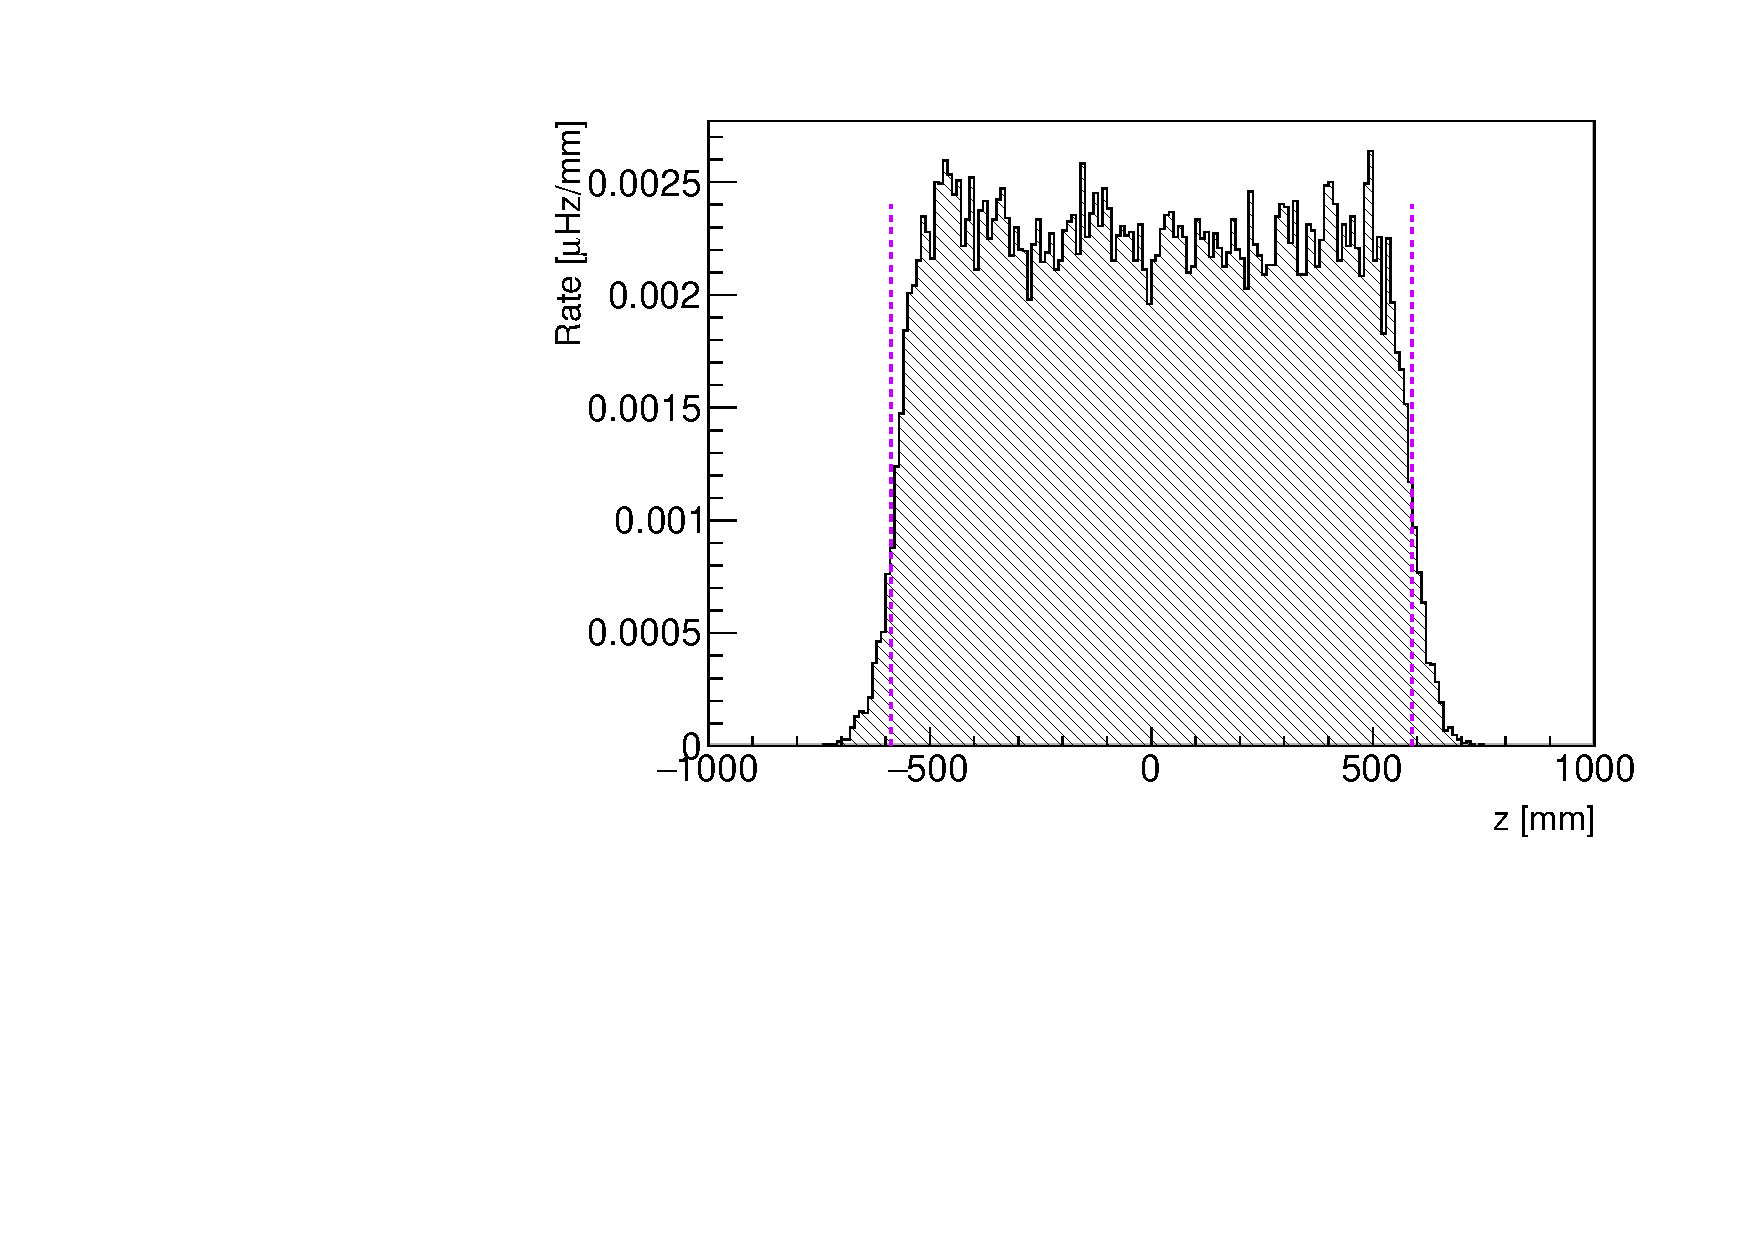
\includegraphics[width=0.6\linewidth]{tex/6-ac227-images/AD_EventSelection/PoPos_Seg76}
	\caption{Reconstructed position distribution for \Po events in a typical segment integrated over all time. Vertical dashed lines (purple) are drawn at the limits of the physical length of the segment.}
	\label{fig:poposseg76}
\end{figure}

\begin{figure}[h]
	\centering
	\begin{subfigure}{0.5\linewidth}
		\centering
		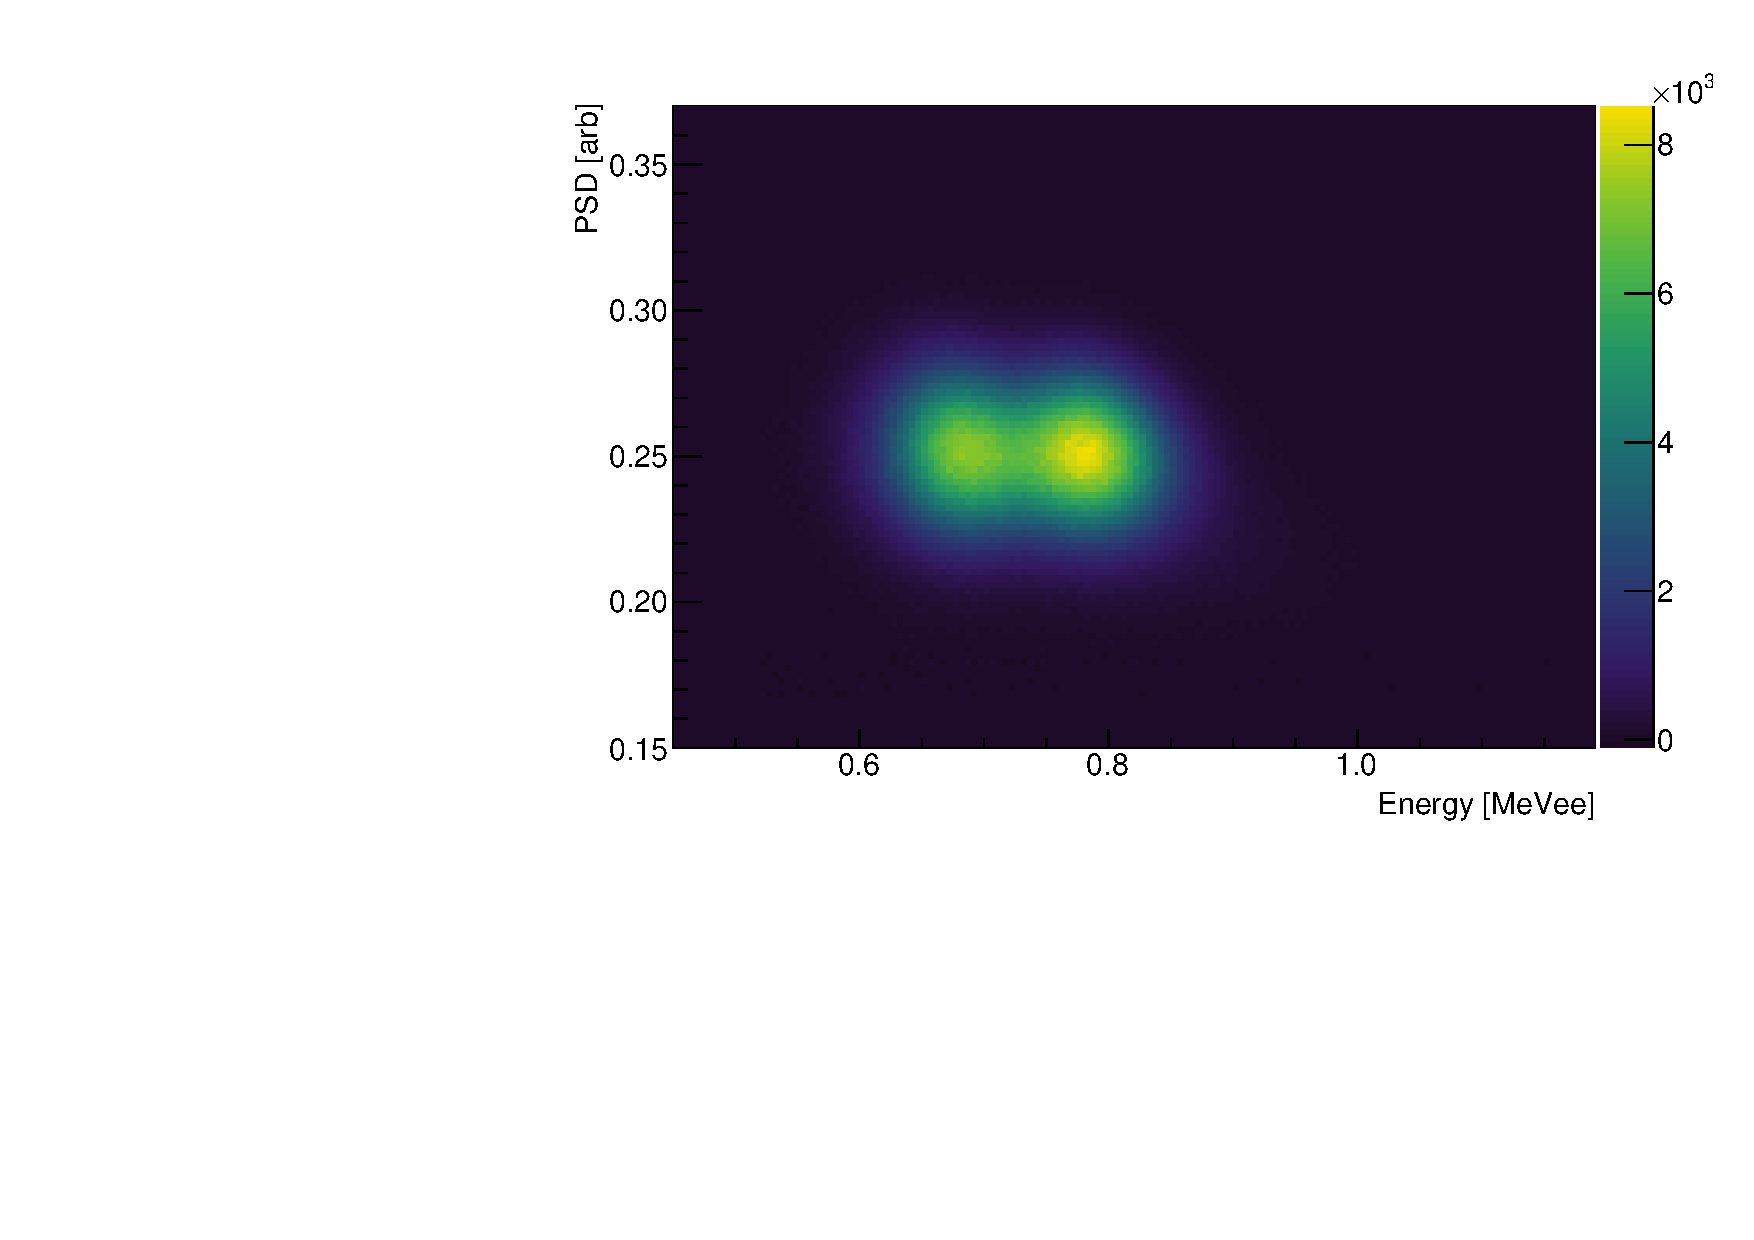
\includegraphics[width=0.9\linewidth]{tex/6-ac227-images/AD_EventSelection/RnPoPSDvsEn_AllCellsAllTime_Time0}
		\caption{RnPo PSD versus Energy.}
		\label{fig:rnpopsdvsentimebin0}
	\end{subfigure}\hspace{0cm}%
	\begin{subfigure}{0.5\linewidth}
		\centering
		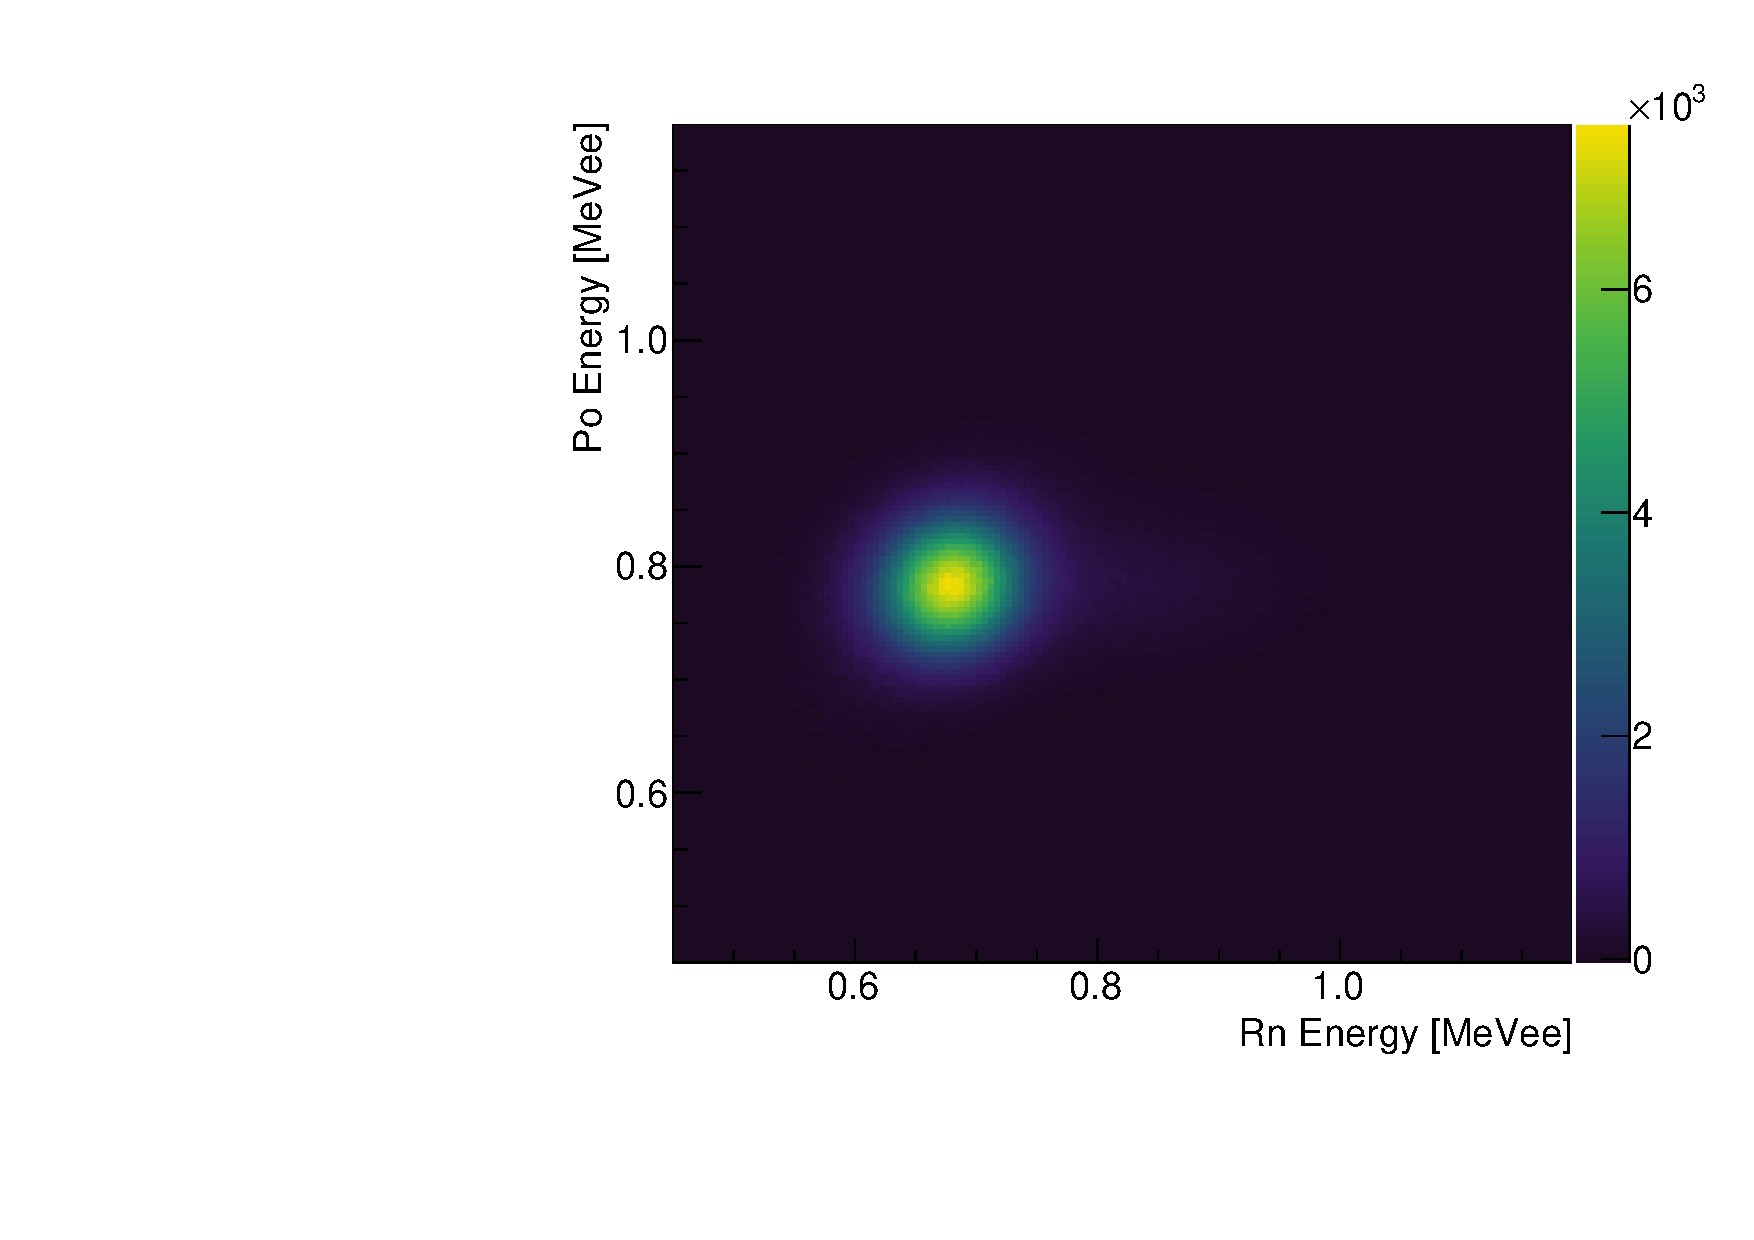
\includegraphics[width=0.7\linewidth]{tex/6-ac227-images/AD_EventSelection/PoEnvsRnEn_AllCellsAllTime_Time0}
		\caption{\Po energy versus \Rn energy.}
		\label{fig:poenvsrnentimebin0}
	\end{subfigure}
	\caption{RnPo distributions for all cells integrated over all time.}
	\label{fig:RnPoPSDEn}
\end{figure}



\subsection{Rate Calculation}

The \Ac rate per segment, or for a given time period, was found by fitting the background subtracted $\Delta t$ distribution, where $\Delta t = t_{\textrm{delay}} - t_{\textrm{prompt}}$, with
\begin{equation}
	f(t) = Ne^{-t/\tau}.
	\label{eq:dtexp}
\end{equation}
where $N$ and $\tau$, the lifetime of $^{215}$Po, were allowed to vary.
For an example of these distributions and fit for a typical segment see Figure~\ref{fig:rnpodtseg76}.
The rate was then calculated as
\begin{equation}
	R = \frac{N~\tau}{\Delta t\textrm{-bin-width}\times\textrm{livetime}\times\textrm{efficiency}},
\end{equation}
\begin{equation}
	\sigma_R = R \times \sqrt{\left(\frac{\sigma_N}{N}\right)^2 + \left(\frac{\sigma_\tau}{\tau}\right)^2  +  \frac{2\sigma_{N\tau}}{N\tau} + \left(\frac{\sigma_{eff.}}{eff.}\right)^2},
\end{equation}
where $N$ and $\tau$ are results of the $\Delta t$ fit.
The robustness of this fit can be tracked by observing the resulting values for $\tau$ per individual segment and versus time for all segments and comparing the averages to the currently accepted value for the lifetime of $^{215}$Po, 2.569 $\pm$ 0.007 ms.
These results are shown in Figure~\ref{fig:tau}.
The average lifetime per individual segment is 2.564 $\pm$ 0.002ms, and versus time for all segments in 2.565 $\pm$ 0.002 ms, in great agreement with the accepted lifetime.

\begin{figure}[h]
	\centering
	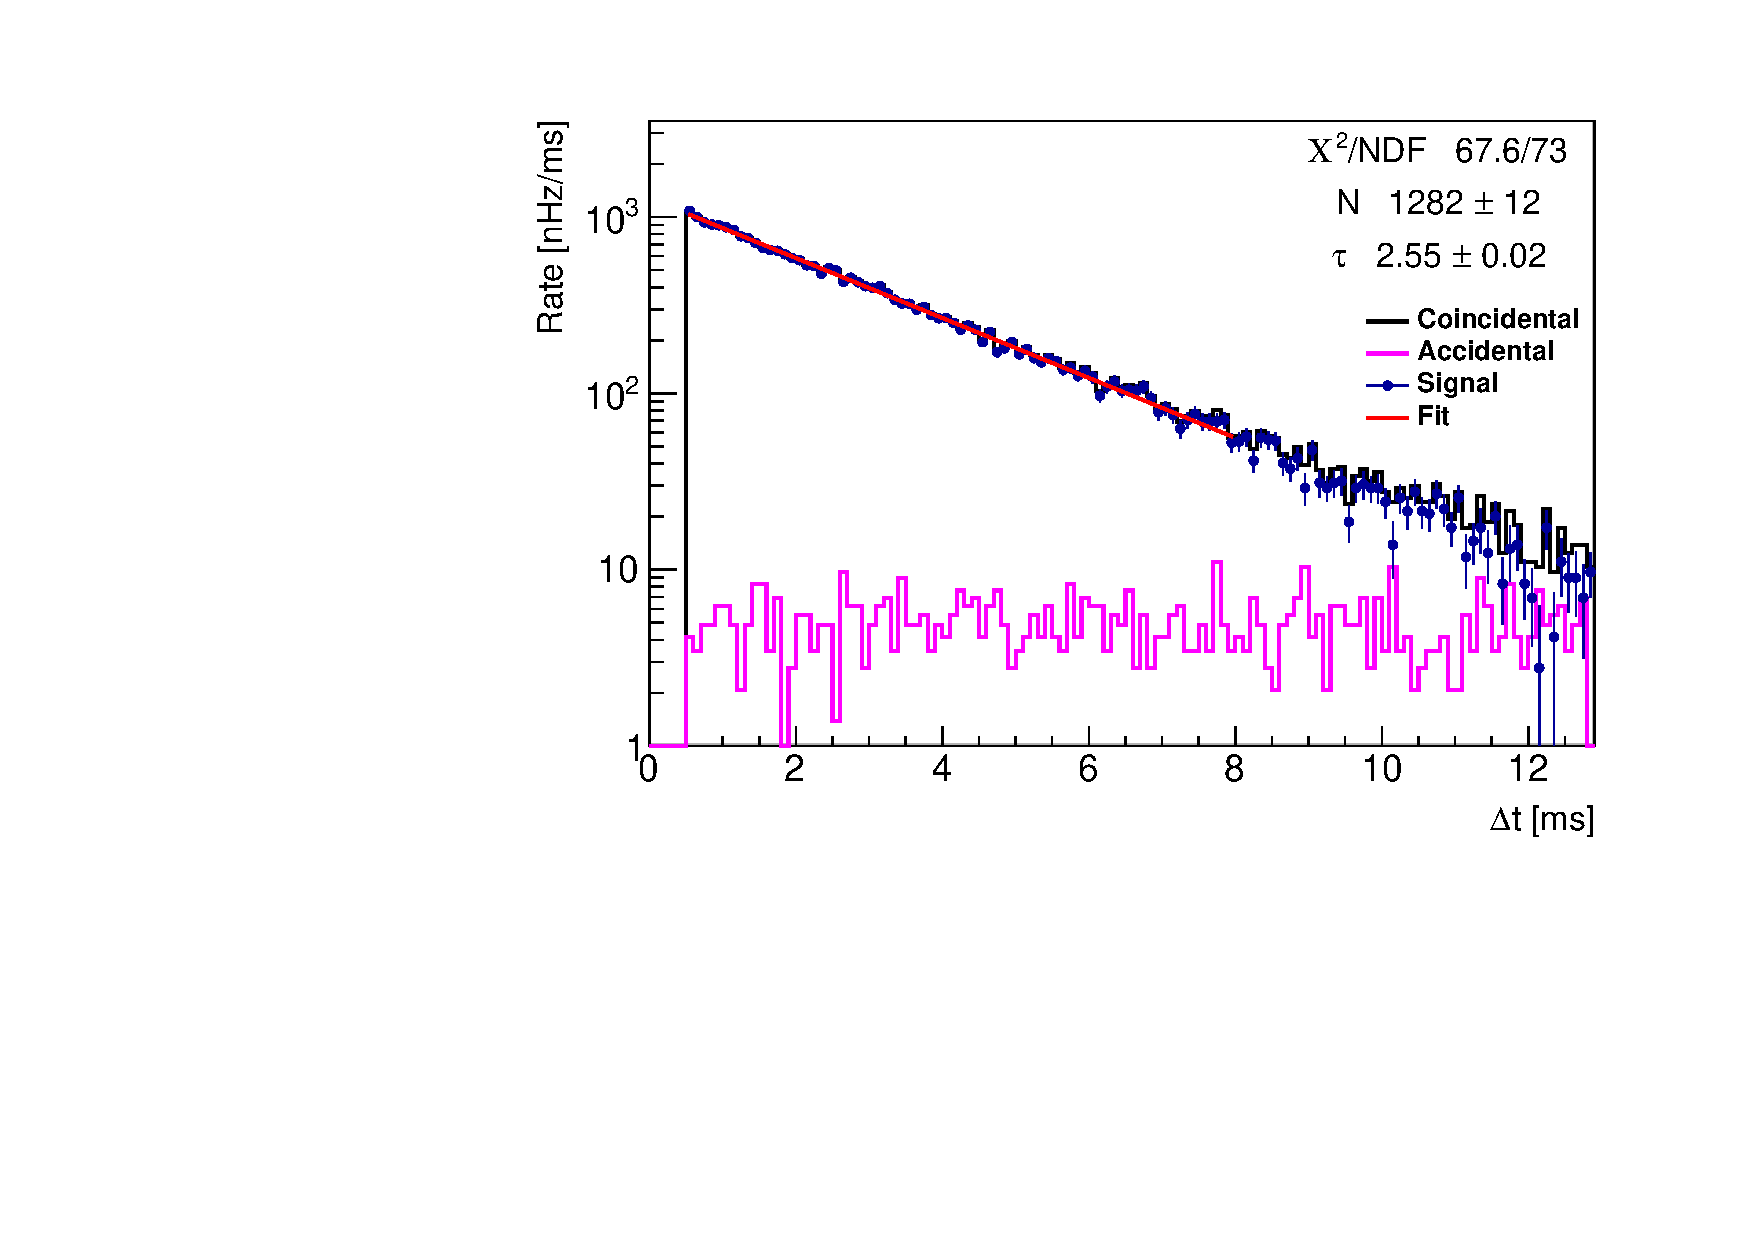
\includegraphics[width=0.65\linewidth]{tex/6-ac227-images/AD_RateCalc/RnPoDt_Seg76}
	\caption{Coincidental (black), accidental (magenta), and background subtracted (blue) $\Delta t$ distributions for a typical segment integrated over all time. A fit of Equation~\ref{eq:dtexp} to the background subtraction distribution is shown in red along with its results.}
	\label{fig:rnpodtseg76}
\end{figure}

\begin{figure}[h]
	\begin{subfigure}{1\linewidth}
	\centering
	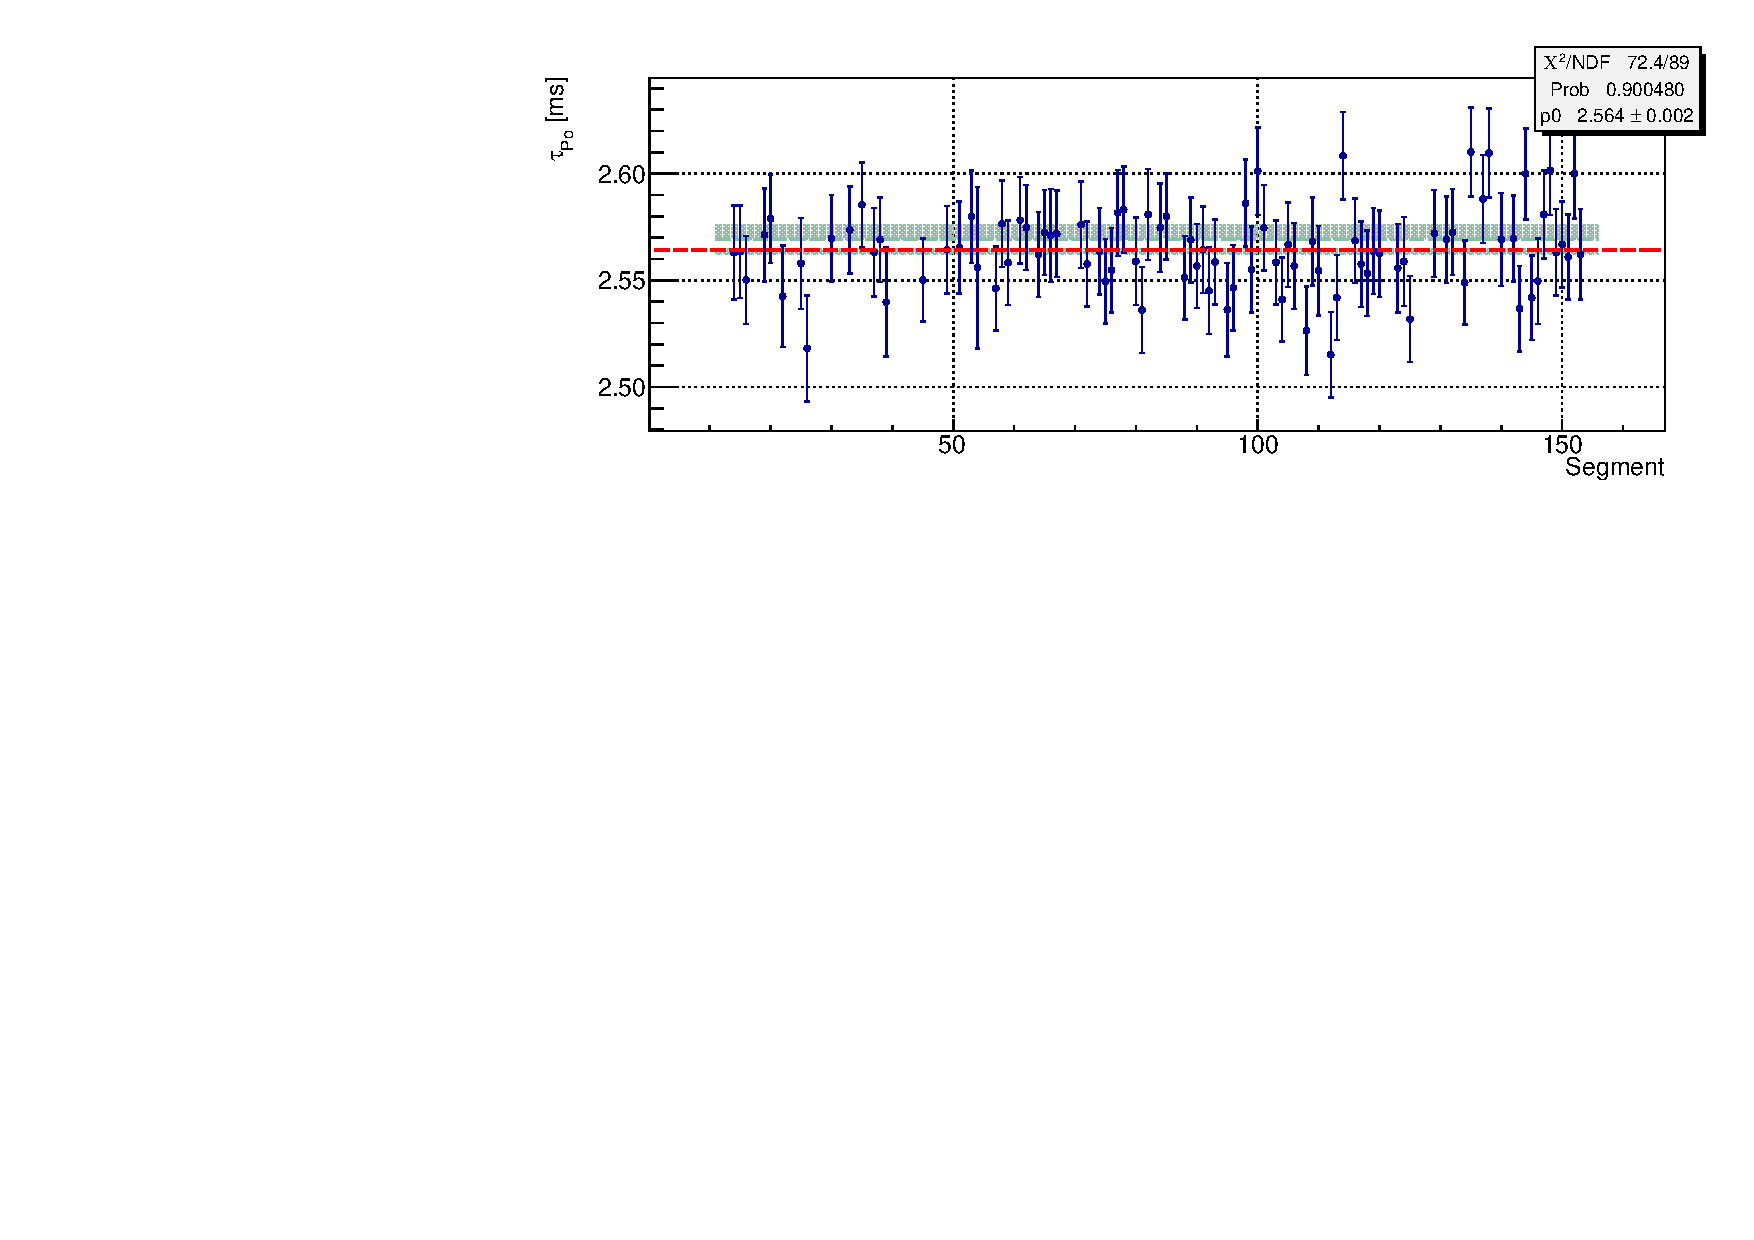
\includegraphics[width=0.8\linewidth]{tex/6-ac227-images/AD_RateCalc/LifetimePerCell}
	\caption{}
	\label{fig:lifetimepercell}
\end{subfigure}
\begin{subfigure}{1\linewidth}
	\centering
	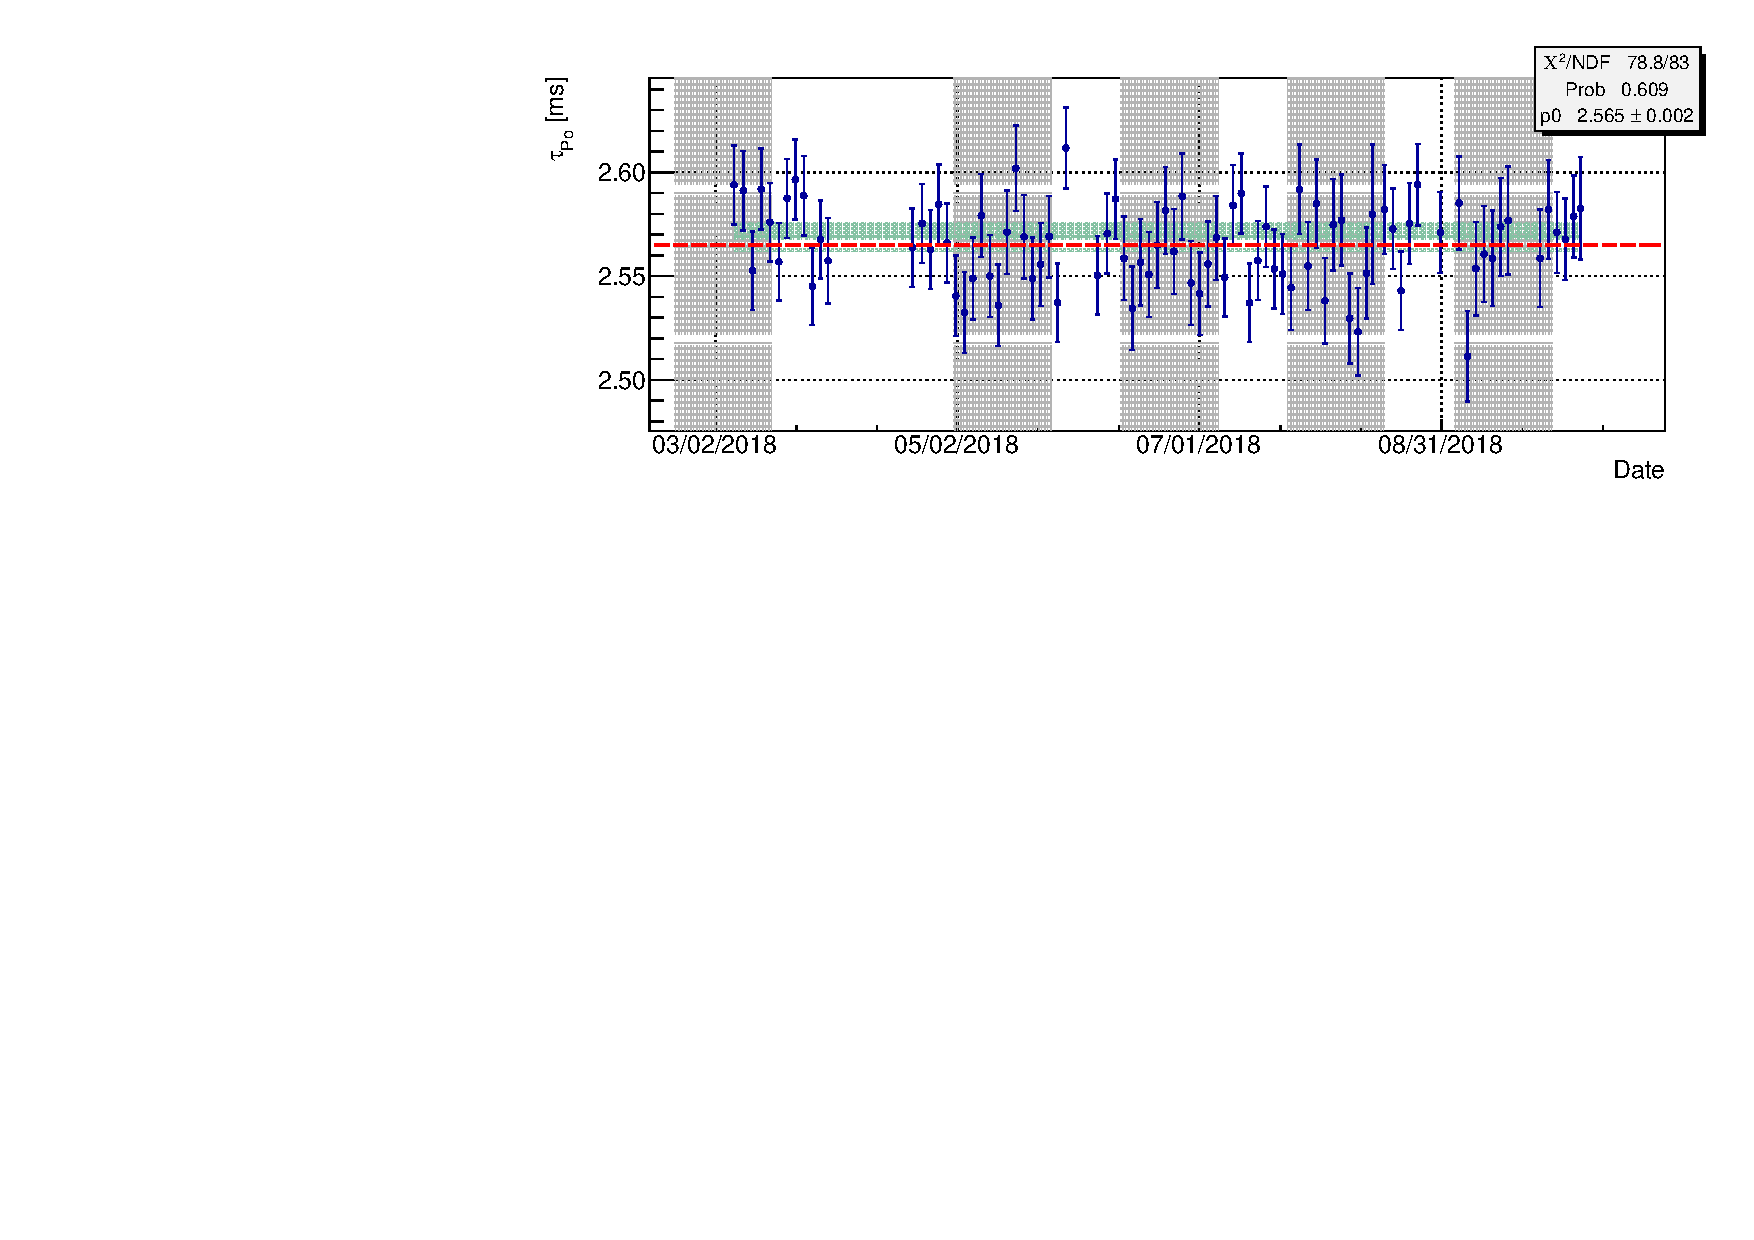
\includegraphics[width=0.8\linewidth]{tex/6-ac227-images/AD_RateCalc/LifetimeVsTime}
	\caption{}
	\label{fig:lifetimevstime}
\end{subfigure}
\caption{The value of $\tau$ obtained from the exponential fit to the $\Delta t$ distribution for each individual segment integrated over all time (a) and for all segments versus time (b). The currently accepted value for $\tau$, 2.569 $\pm$ 0.007 ms, is marked by the shaded green area. A constant fit to the data is shown as the dashed red line. Shaded gray regions in time are reactor on periods.}
\label{fig:tau}
\end{figure}

The uncorrected livetime is calculated, for each data run, as the time from the beginning of the run to the time of the last delay candidate event. 
This is summed for all analyzed runs. 
This livetime was corrected for the dead time introduced by the pileup veto, the software veto imposed before each event to remove issues from hardware triggering and overlapping waveforms that happen when two events are too close to each other in time.
This correction was calculated as the number of clusters, $NClusts$, times the pileup veto time, 800 ns.
Figure~\ref{fig:vetotimevstime} shows the dead time, as a fraction of livetime, versus time.
Because the veto was applied to both prompt and delay candidates the livetime is corrected with 2$\times$ the dead time as
\begin{equation}
	\textrm{livetime} = \sum(t_{\textrm{finalPo}} - t_0) - 2.0 \times NClusts \times 800~\textrm{ns}.
\end{equation}
When measuring the rate per segment the same livetime was applied to all segments. 

\begin{figure}[!t]
	\centering
	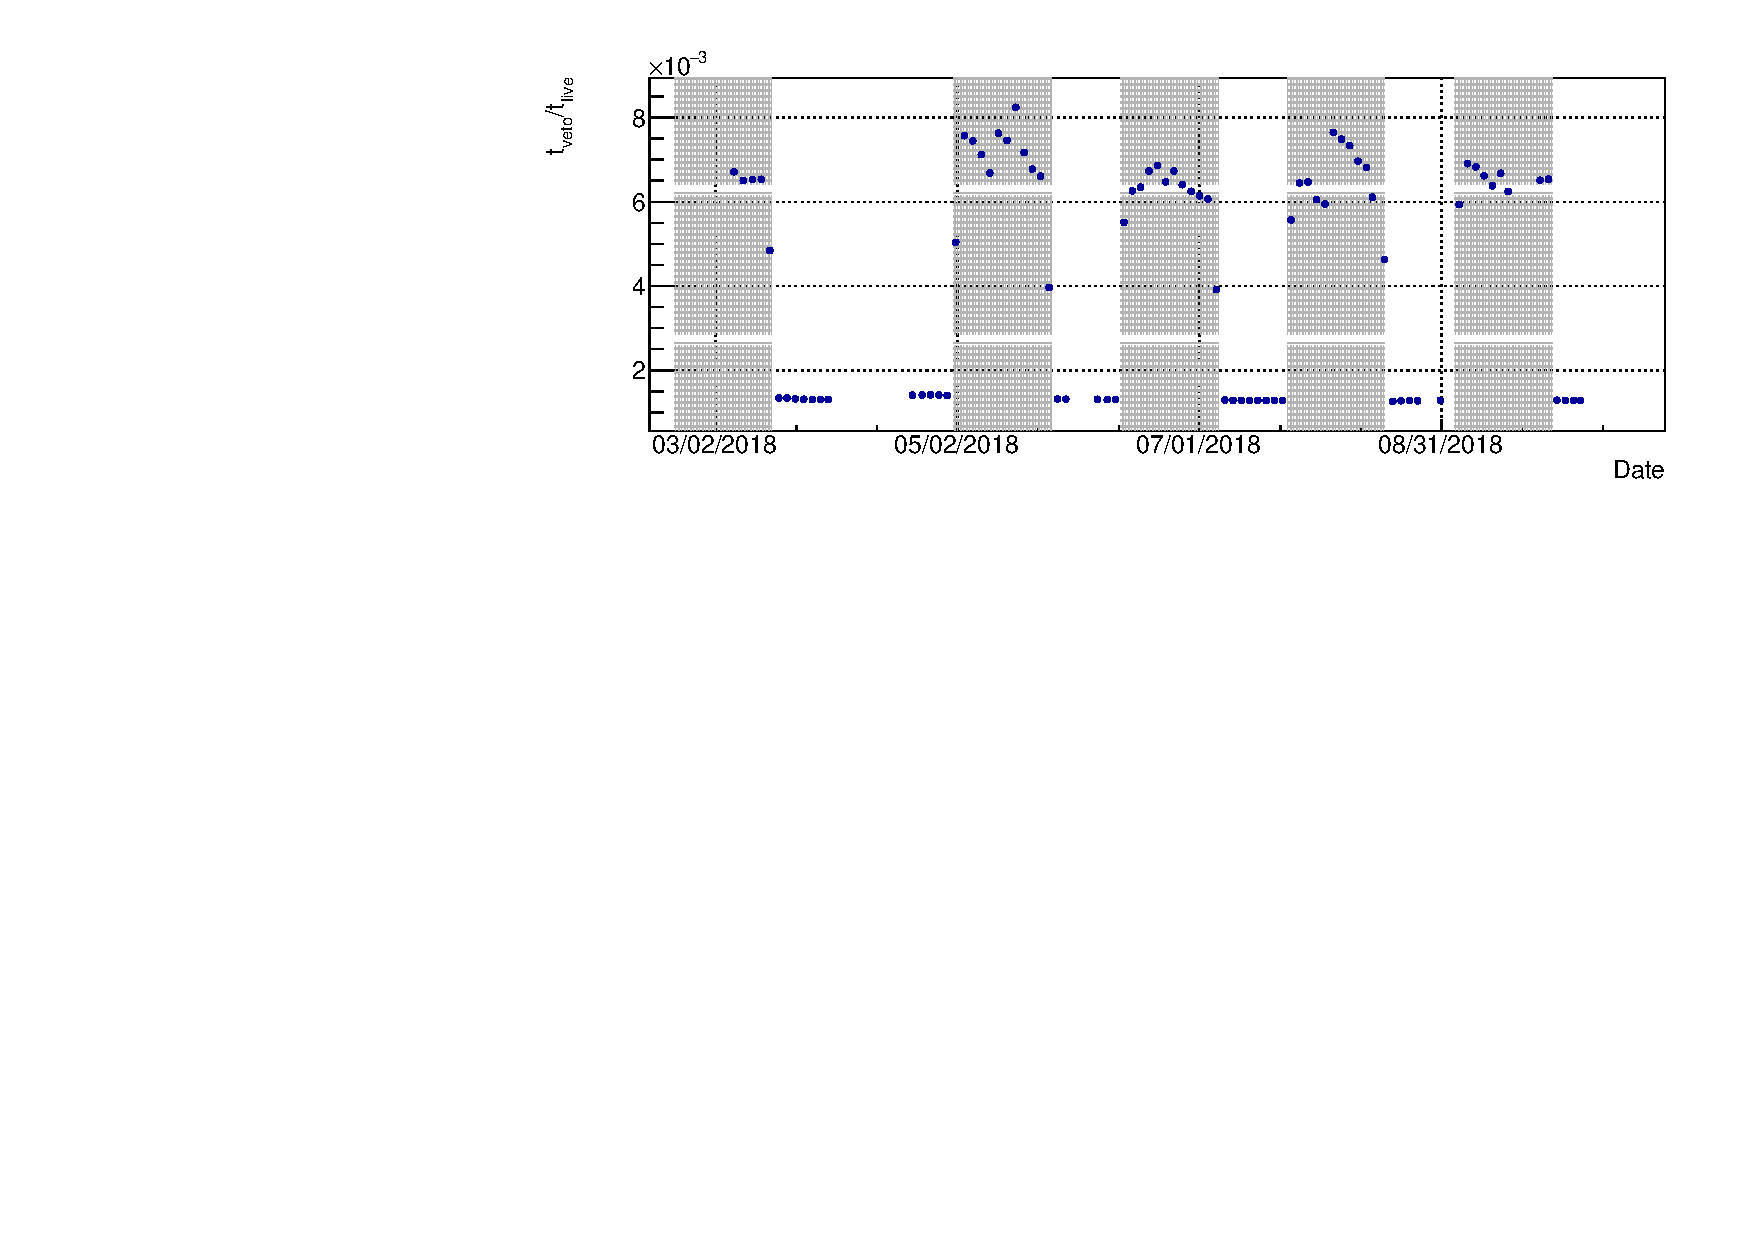
\includegraphics[width=0.8\linewidth]{tex/6-ac227-images/AD_RateCalc/VetoTimeVsTime}
	\caption{The dead time, as a fraction of livetime, due to the pileup veto versus time. Shaded areas are reactor on periods.}
	\label{fig:vetotimevstime}
\end{figure}

The efficiency was calculated for energy and PSD cuts on both prompt and delay events, and for the $\Delta z$ cut.
This was done by fitting each distribution with a Gaussian $\pm 2\sigma$ from the mean.
This is true for all distributions expect the prompt energy, which has a non-Gaussian high energy tail due to its accompanying gammas, see Figure~\ref{fig:rnpoenseg76}. 
Since the high energy cut was always wide enough to include the whole range of this tail, we only care about the low energy cut, which we can approximate with a Gaussian.
Therefore, prompt energy was fit with a Gaussian from -1.3$\sigma$ to +0.6$\sigma$.
The efficiency was then calculated as the ratio of the integral of the Gaussian
between the cuts for that distribution to the integral between $\pm \infty$, as defined in Equation~\ref{eq:Eff}.
The error on the efficiency was treated as a binomial error.
For an example of the distributions and fits for a typical segment see Figure~\ref{fig:RnPoDist}.

\begin{align}
	\text{Eff} = \frac{\int_{\text{low-cut}}^{\text{high-cut}}g(u) du}{\int_{-\infty}^{\infty}g(u) du},
	&& \sigma_{\text{Eff}} =\sqrt{\frac{\text{Eff}(1-\text{Eff})}{N}},
	\label{eq:Eff}
\end{align}	

In general the total efficiency was 99.9\% or higher, for RnPo rates calculated in individual segments and versus time.
Figures~\ref{fig:efficiencypercell} and \ref{fig:efficiencyvstime} show the efficiency calculated for all distributions for all individual segments and versus time, respectively.
See Table~\ref{tab:Cuts} for a summary of all cuts and their average efficiencies.

\begin{figure}[H]
	\begin{subfigure}{0.5\linewidth}
	\centering
	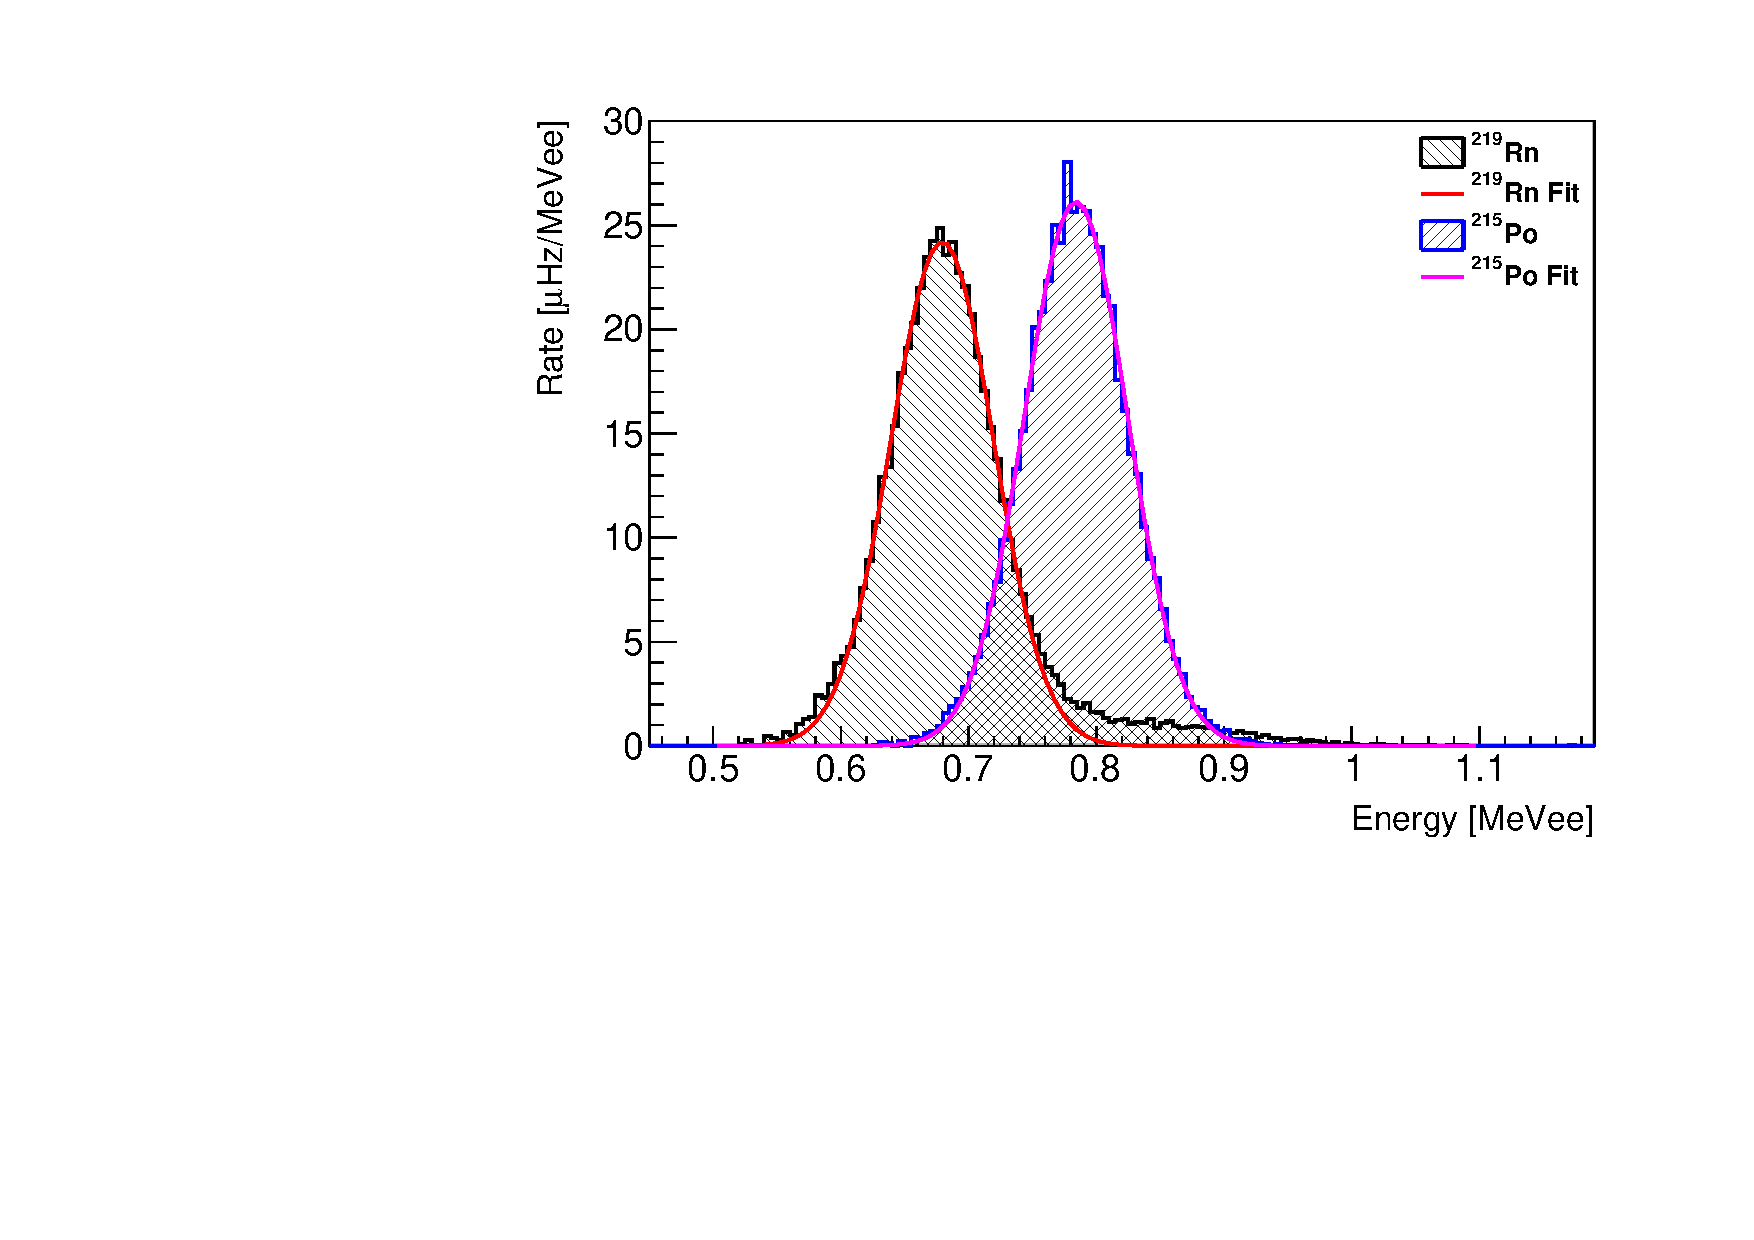
\includegraphics[width=0.95\linewidth]{tex/6-ac227-images/AD_RateCalc/RnPoEn_Seg76}
	\caption{}
	\label{fig:rnpoenseg76}
\end{subfigure}%
\begin{subfigure}{0.5\linewidth}
	\centering
	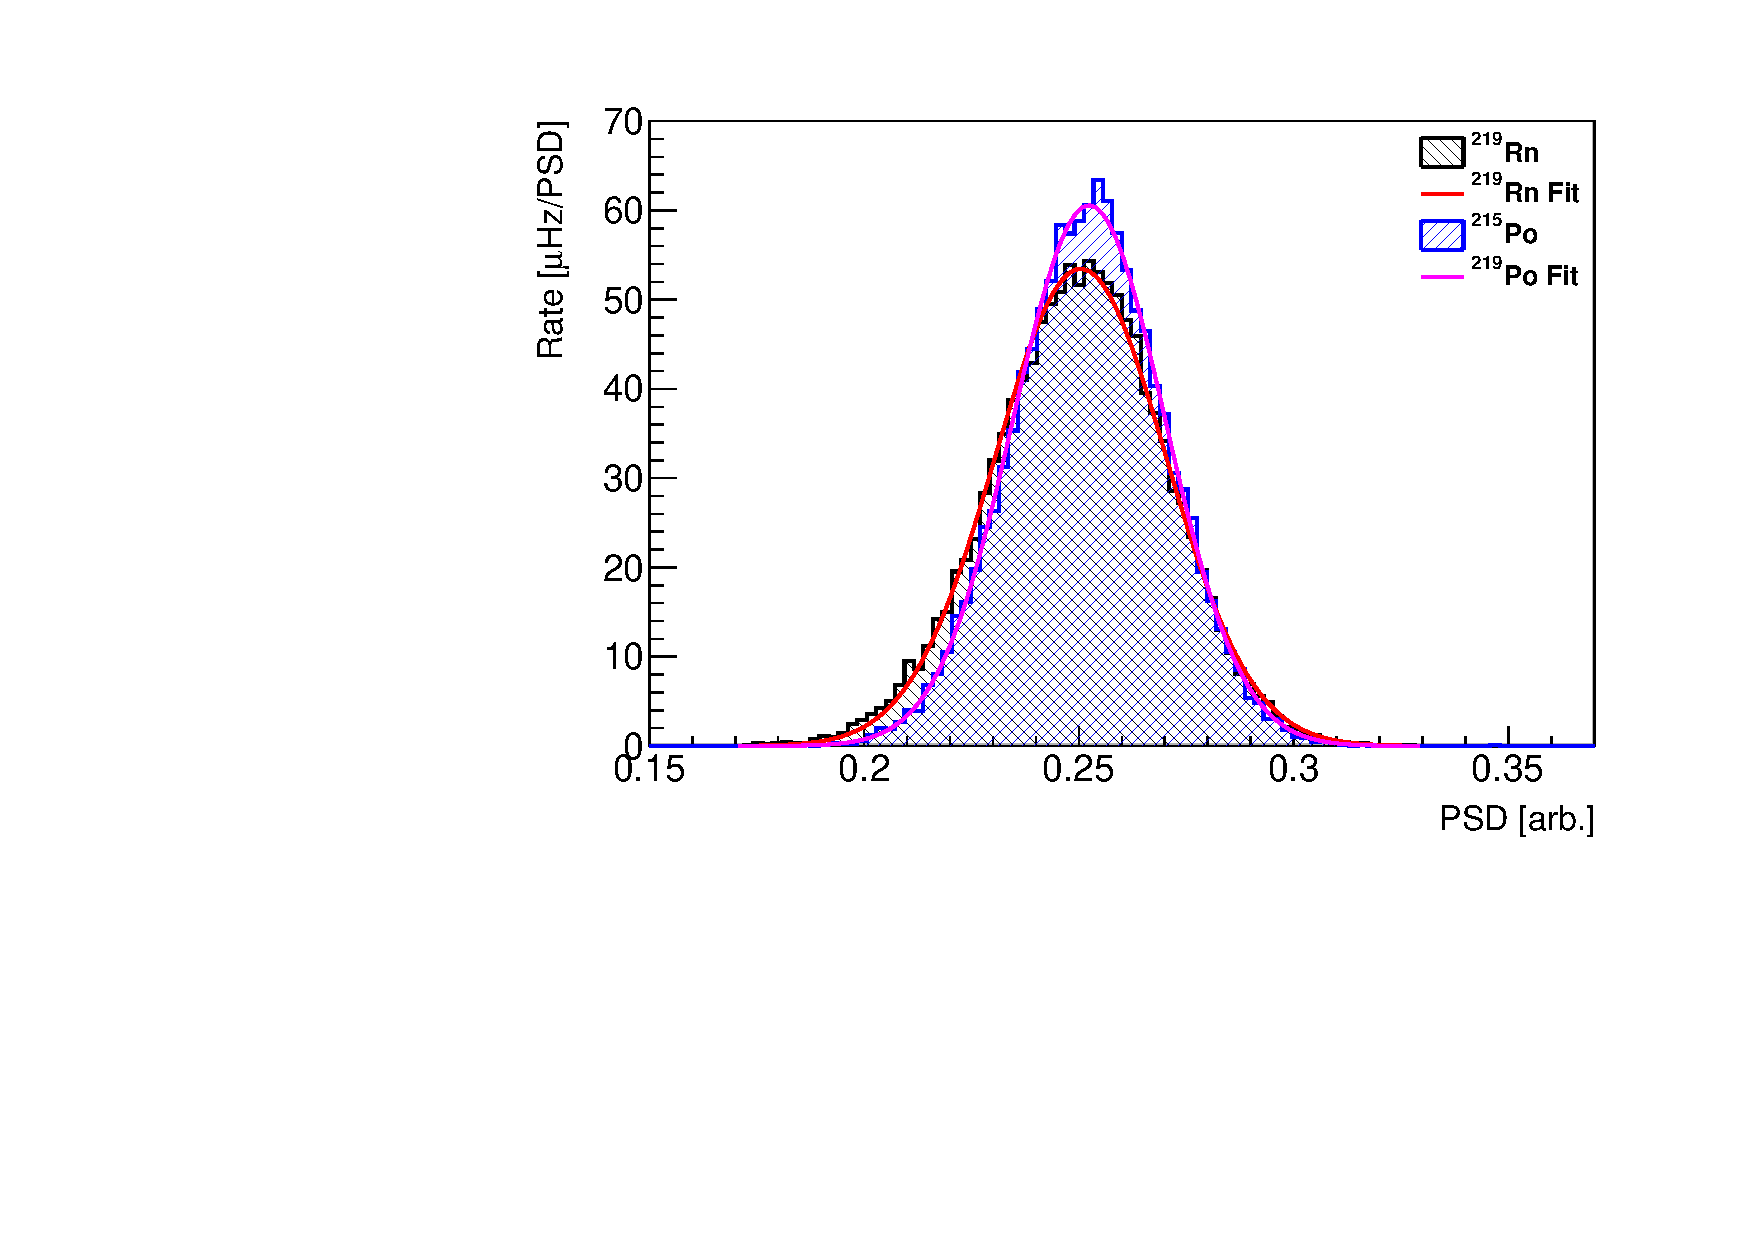
\includegraphics[width=0.95\linewidth]{tex/6-ac227-images/AD_RateCalc/RnPoPSD_Seg76}
	\caption{}
	\label{fig:rnpopsdseg76}
\end{subfigure}
\begin{subfigure}{1\linewidth}
	\centering
	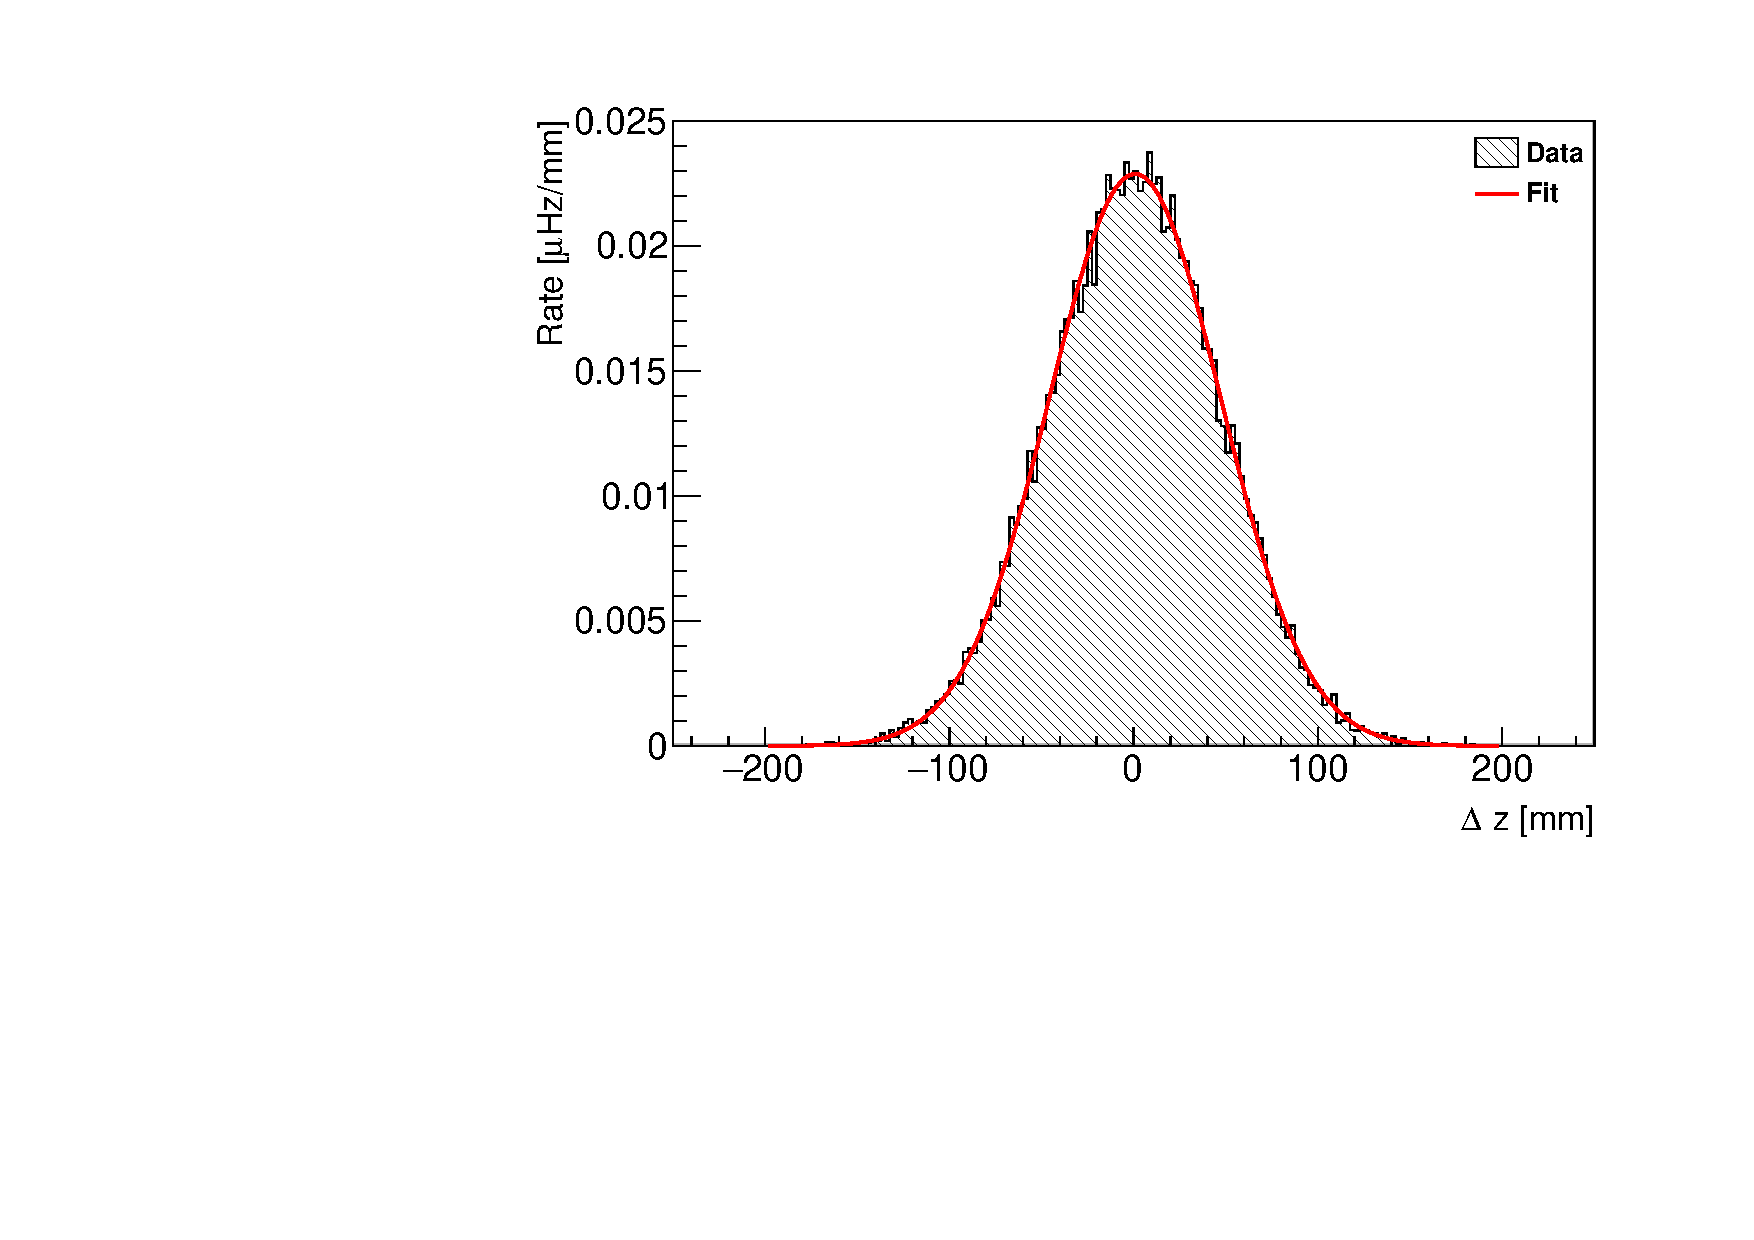
\includegraphics[width=0.475\linewidth]{tex/6-ac227-images/AD_RateCalc/RnPoDz_Seg76}
	\caption{}
	\label{fig:rnpodzseg76}
\end{subfigure}
\caption{Energy (a), PSD (b), and $\Delta z$ (c) distributions for RnPo events in a typical segment integrated over all time. Also shown are the results of fitting each distribution with a Gaussian for the purpose of calculating the cut efficiencies.}
\label{fig:RnPoDist}
\end{figure}

\begin{figure}[h]
	\centering
	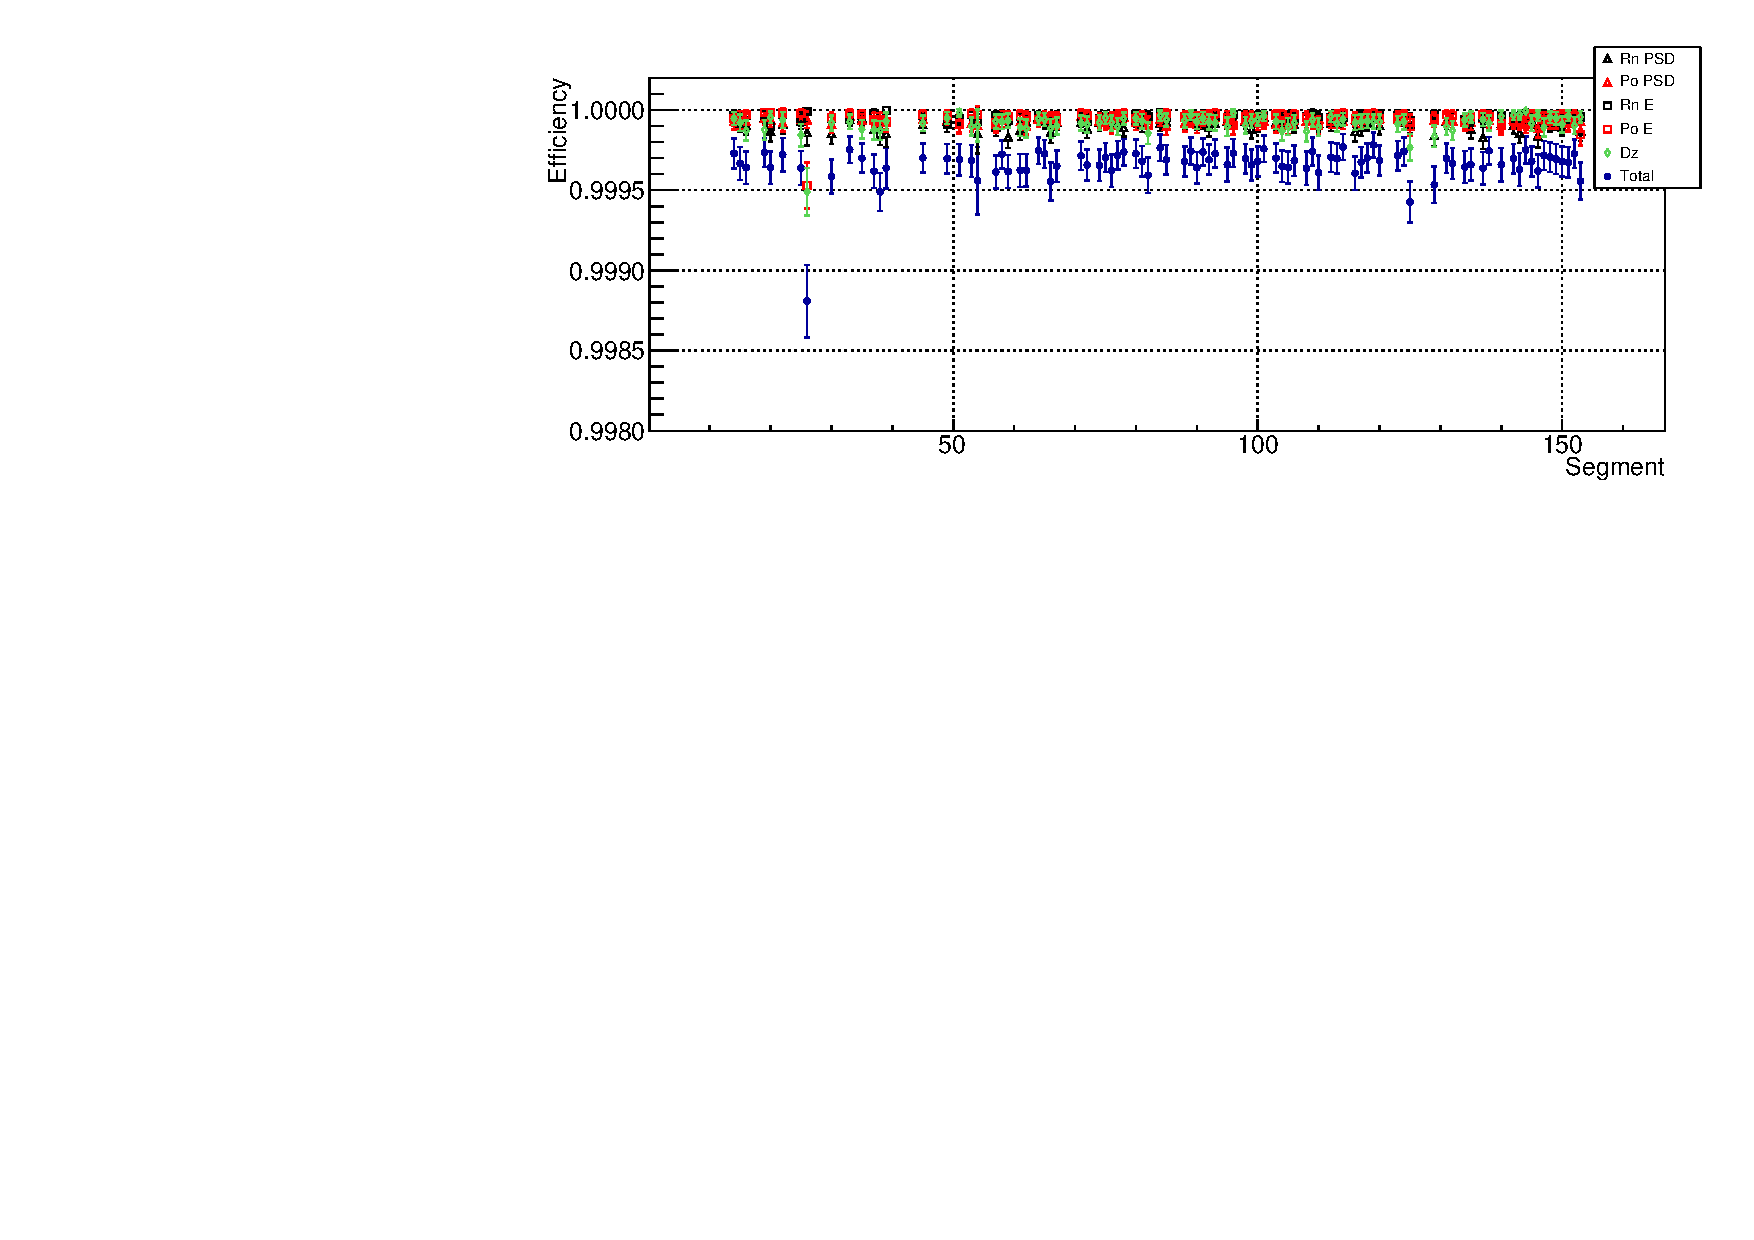
\includegraphics[width=0.9\linewidth]{tex/6-ac227-images/AD_RateCalc/EfficiencyPerCell}
	\caption{Cut efficiencies calculated for RnPo events in individual segments integrated over all time.}
	\label{fig:efficiencypercell}
\end{figure}

\begin{figure}[h]
	\centering
	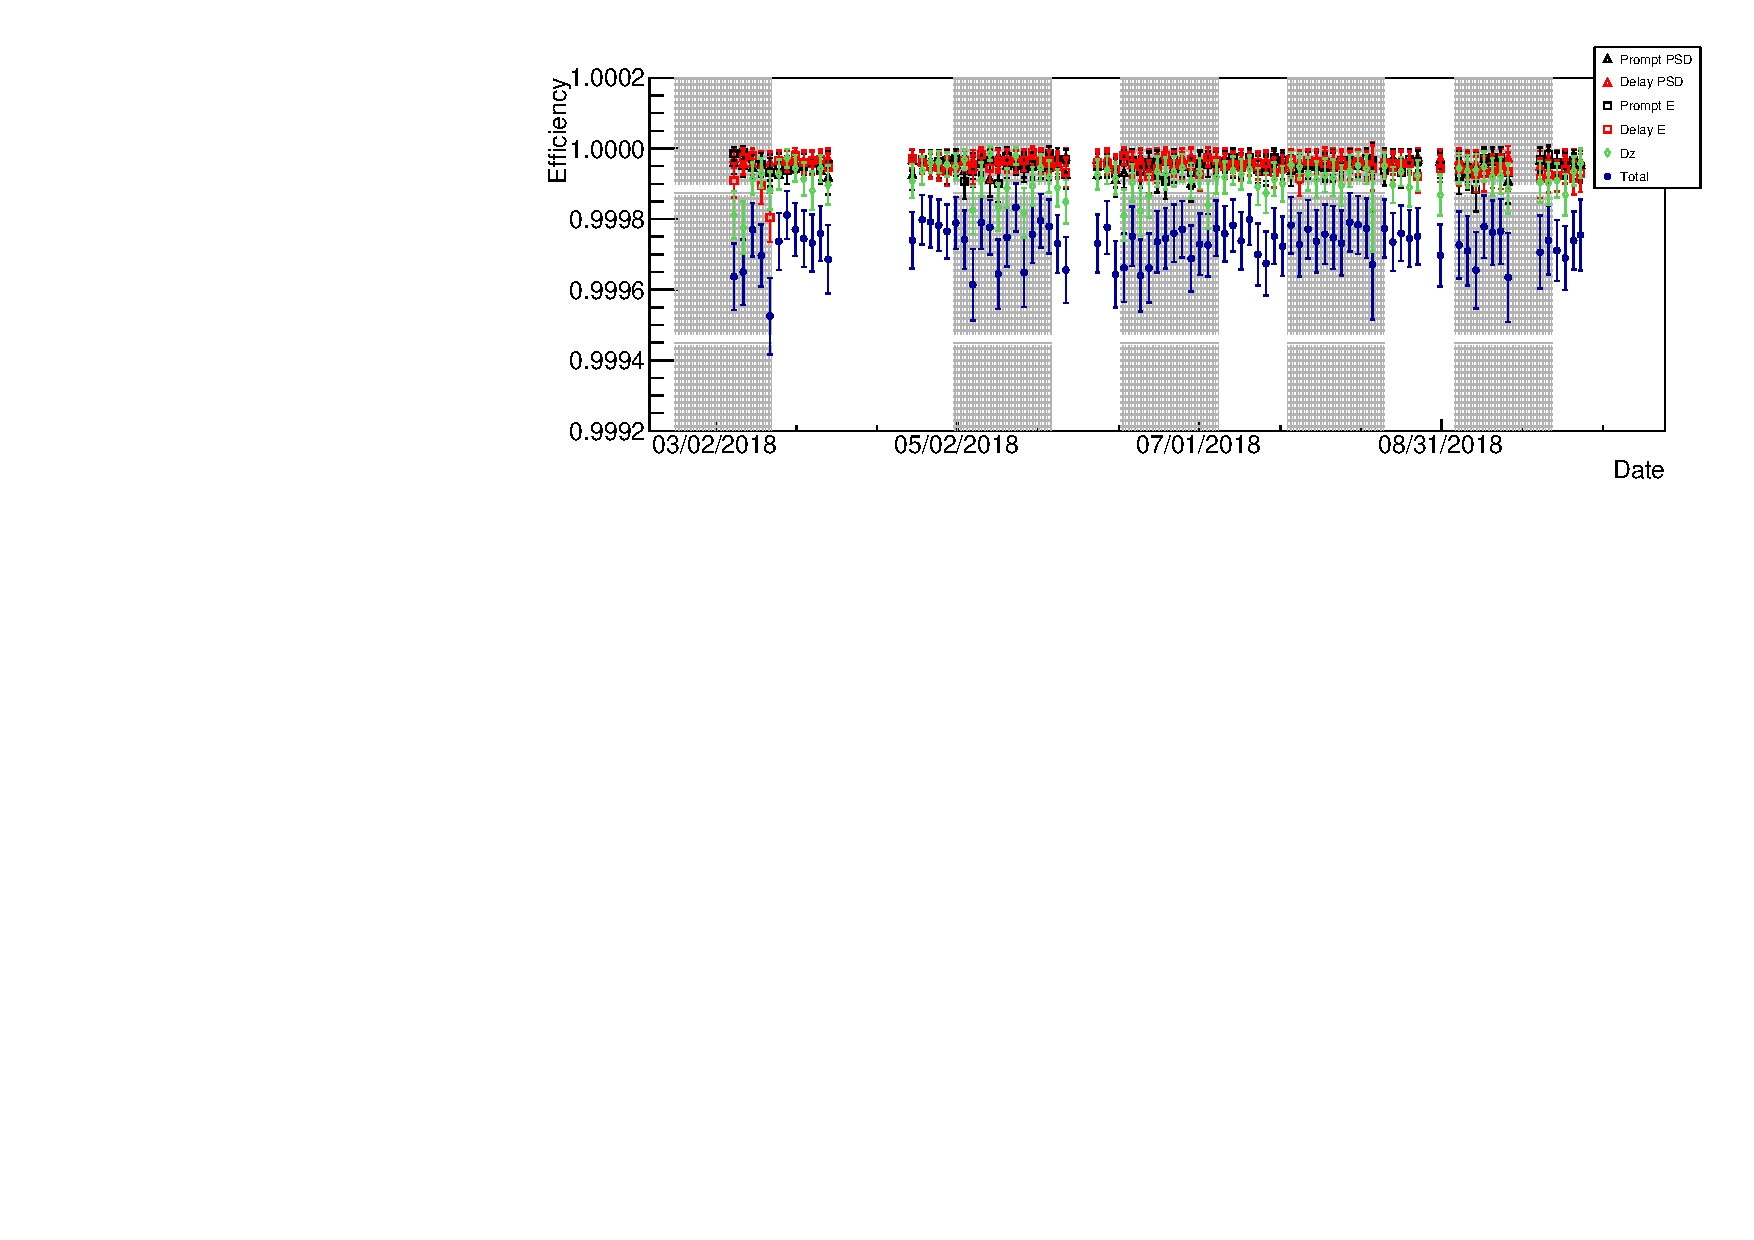
\includegraphics[width=0.9\linewidth]{tex/6-ac227-images/AD_RateCalc/EfficiencyVsTime}
	\caption{Cut efficiencies calculated for RnPo events versus time integrated over all segments. Shaded areas are reactor on periods.}
	\label{fig:efficiencyvstime}
\end{figure}

\begin{table}[H]
	\centering
	\begin{tabular}{c|c|c|c}
		\hline
		\textbf{Cut}         & \textbf{Range} & \textbf{$\langle$Eff$_{\text{Cell}}\rangle$\%} & \textbf{$\langle$Eff$_{\text{Time}}\rangle$\%} \\ \hline
		Pileup veto & Veto any cluster preceded             &   & \\ 
		& less than 800 ns by another cluster   &   & \\ \hline
		PSD         & $\mu - 4\sigma < \text{PSD}_{\text{Rn}} <$ 0.36 & 99.993  & 99.996 \\ 
		& $\mu - 4\sigma < \text{PSD}_{\text{Po}} <$ 0.36 & 99.994  & 99.997 \\ \hline
		Energy      & $\mu - 4\sigma < \text{E}_{\text{Rn}} <$ 1.18 MeV & 99.997  & 99.996  \\
		& $\mu - 4\sigma < \text{E}_{\text{Po}} <$ 1.18 MeV & 99.996  & 99.996 \\ \hline
		Position    & -1000 $< \text{z}_{\text{Rn/Po}} <$ 1000 mm &    &   \\ 
		& Segment-Rn = Segment-Po & & \\ \hline
		$\Delta$z   & $\mu - 4\sigma < \Delta \text{z} < \mu + 4\sigma$   & 99.994   & 99.993  \\ \hline
		$\Delta$t   & $0.5 < \Delta \text{t} < 12.845$ ms &  &   \\ \hline
	\end{tabular}
	\caption{Summary of the chosen cuts and their average efficiencies for determining the \Ac rate in the PROSPECT AD. The means and sigmas are determined by fitting the peaks of all distributions with Gaussians. They are found for each individual segment or each individual time bin (depending on the analysis being done). Average efficiencies are found by fitting the data in Figures~\ref{fig:efficiencypercell} and \ref{fig:efficiencyvstime} with constants.}
	\label{tab:Cuts}
\end{table}


\subsection{Detector Performance as Tracked with \Ac}

Though \Ac was added to the detector in order to measure relative segment-to-segment volume variations, the mono-energetic \Po $\alpha$ was also useful for tracking the performance of the detector and the applied calibrations.
Figure~\ref{fig:EvsT} shows the mean and 1$\sigma$ width of the \Po energy distribution versus time, integrated over all segments. 
It can be seen that the resolution was not stable over time, but rather decreased by $\sim$20\% over a period of 7 months.
This is due to an overall decrease in light collection over time, implying some factor of scintillator degradation such as a loss of transparency or light production, whose cause is not yet understood.

To correct for this in the IBD analysis a variable called $E_{smear}$ was introduced, in which all energy distributions were smeared by artificially adding random noise at the software level to match the worst resolution in a given data taking period.
The results of this are also shown in Figure~\ref{fig:EvsT}, and it can be seen that the new $E_{smear}$ resolution values were time-stable within $\pm$3\% and the mean values within $\pm$0.4\%.
Note that the sharp variations in the energy mean values correspond to times when a new set of calibration constants were introduced in the analysis.

Though introducing the $E_{smear}$ variable corrected for changing detector characteristics, the \Ac analysis used $E$. 
The decreasing resolution was accounted for by applying $\sigma$-based cuts to the energy.

\begin{figure}[h]
\begin{subfigure}{1\linewidth}
	\centering
	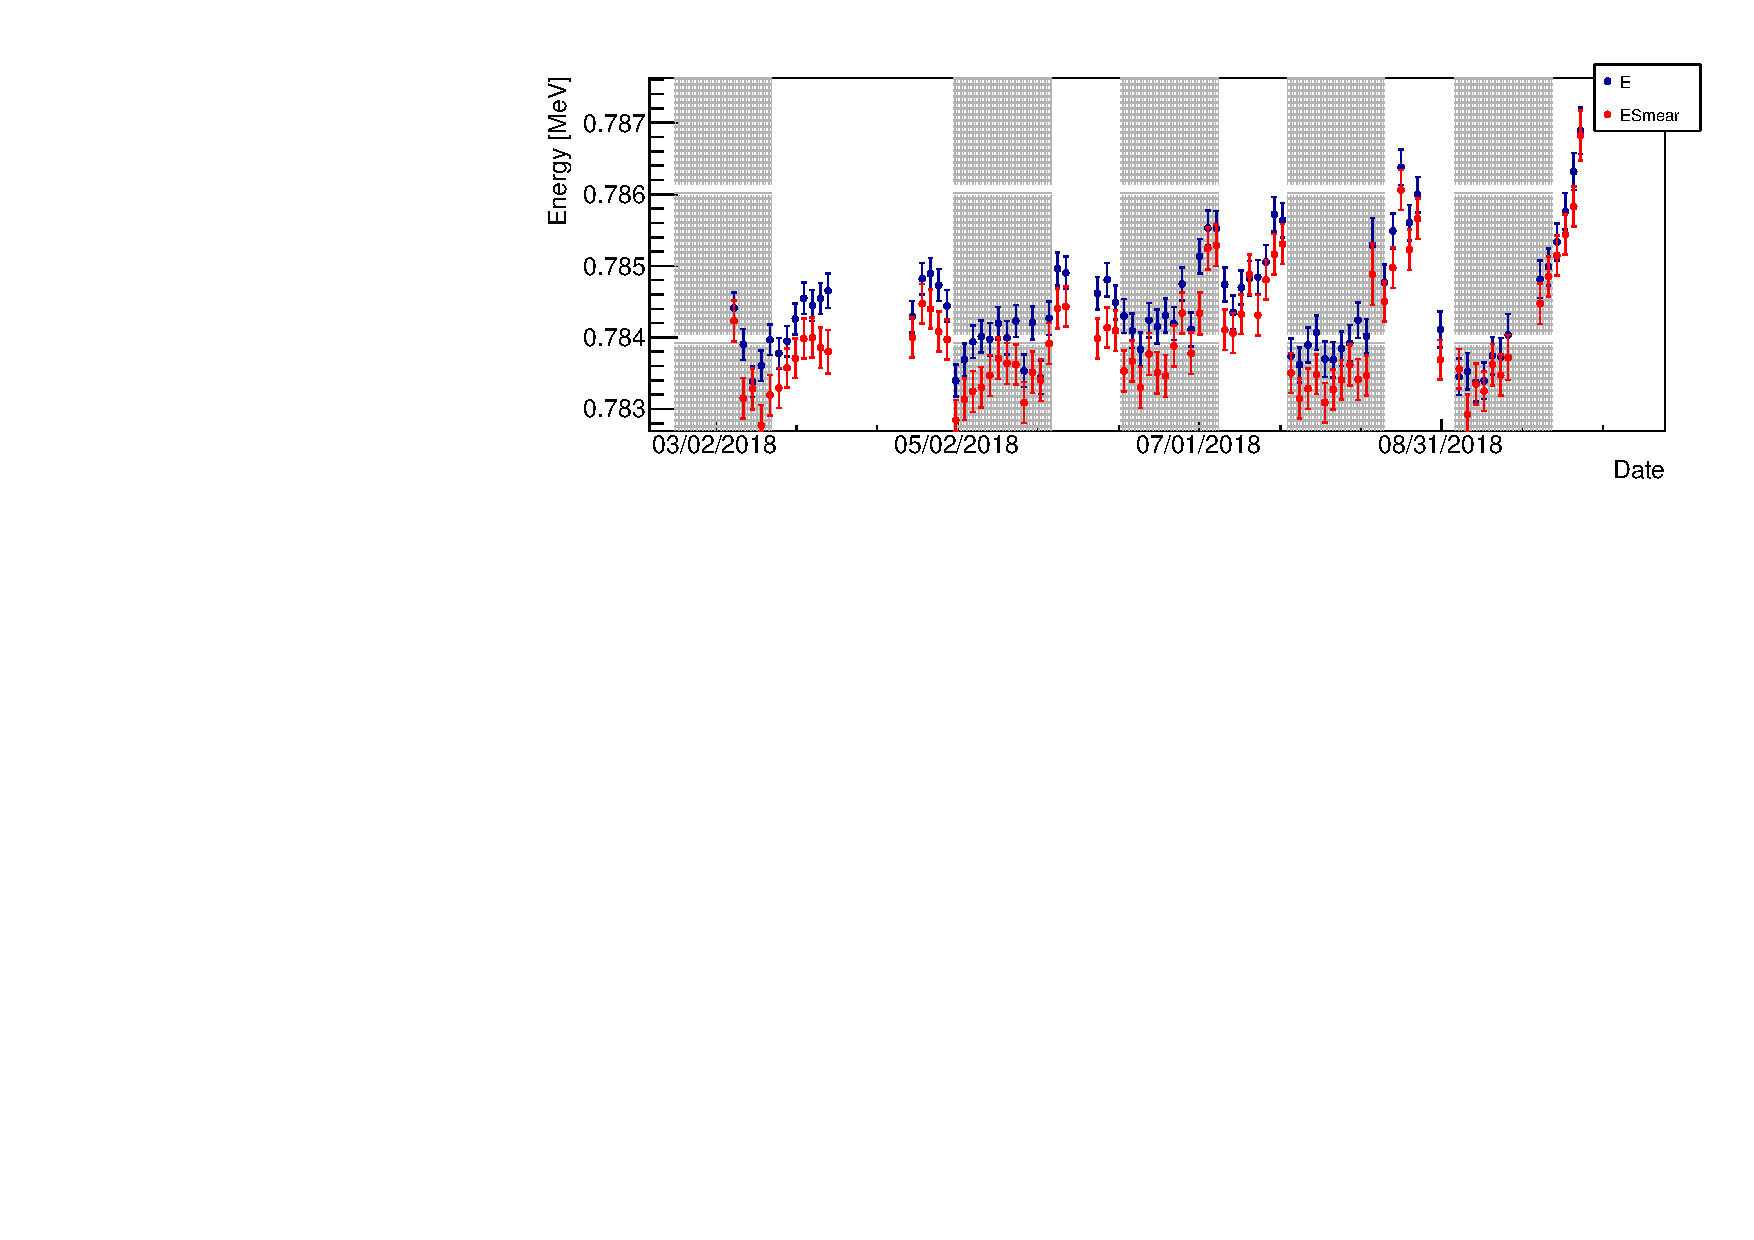
\includegraphics[width=0.9\linewidth]{tex/6-ac227-images/DetPerformance/PoEnMeanVsTime}
	\caption{}
	\label{fig:poenmeanvstime}
\end{subfigure}
\begin{subfigure}{1\linewidth}
	\centering
	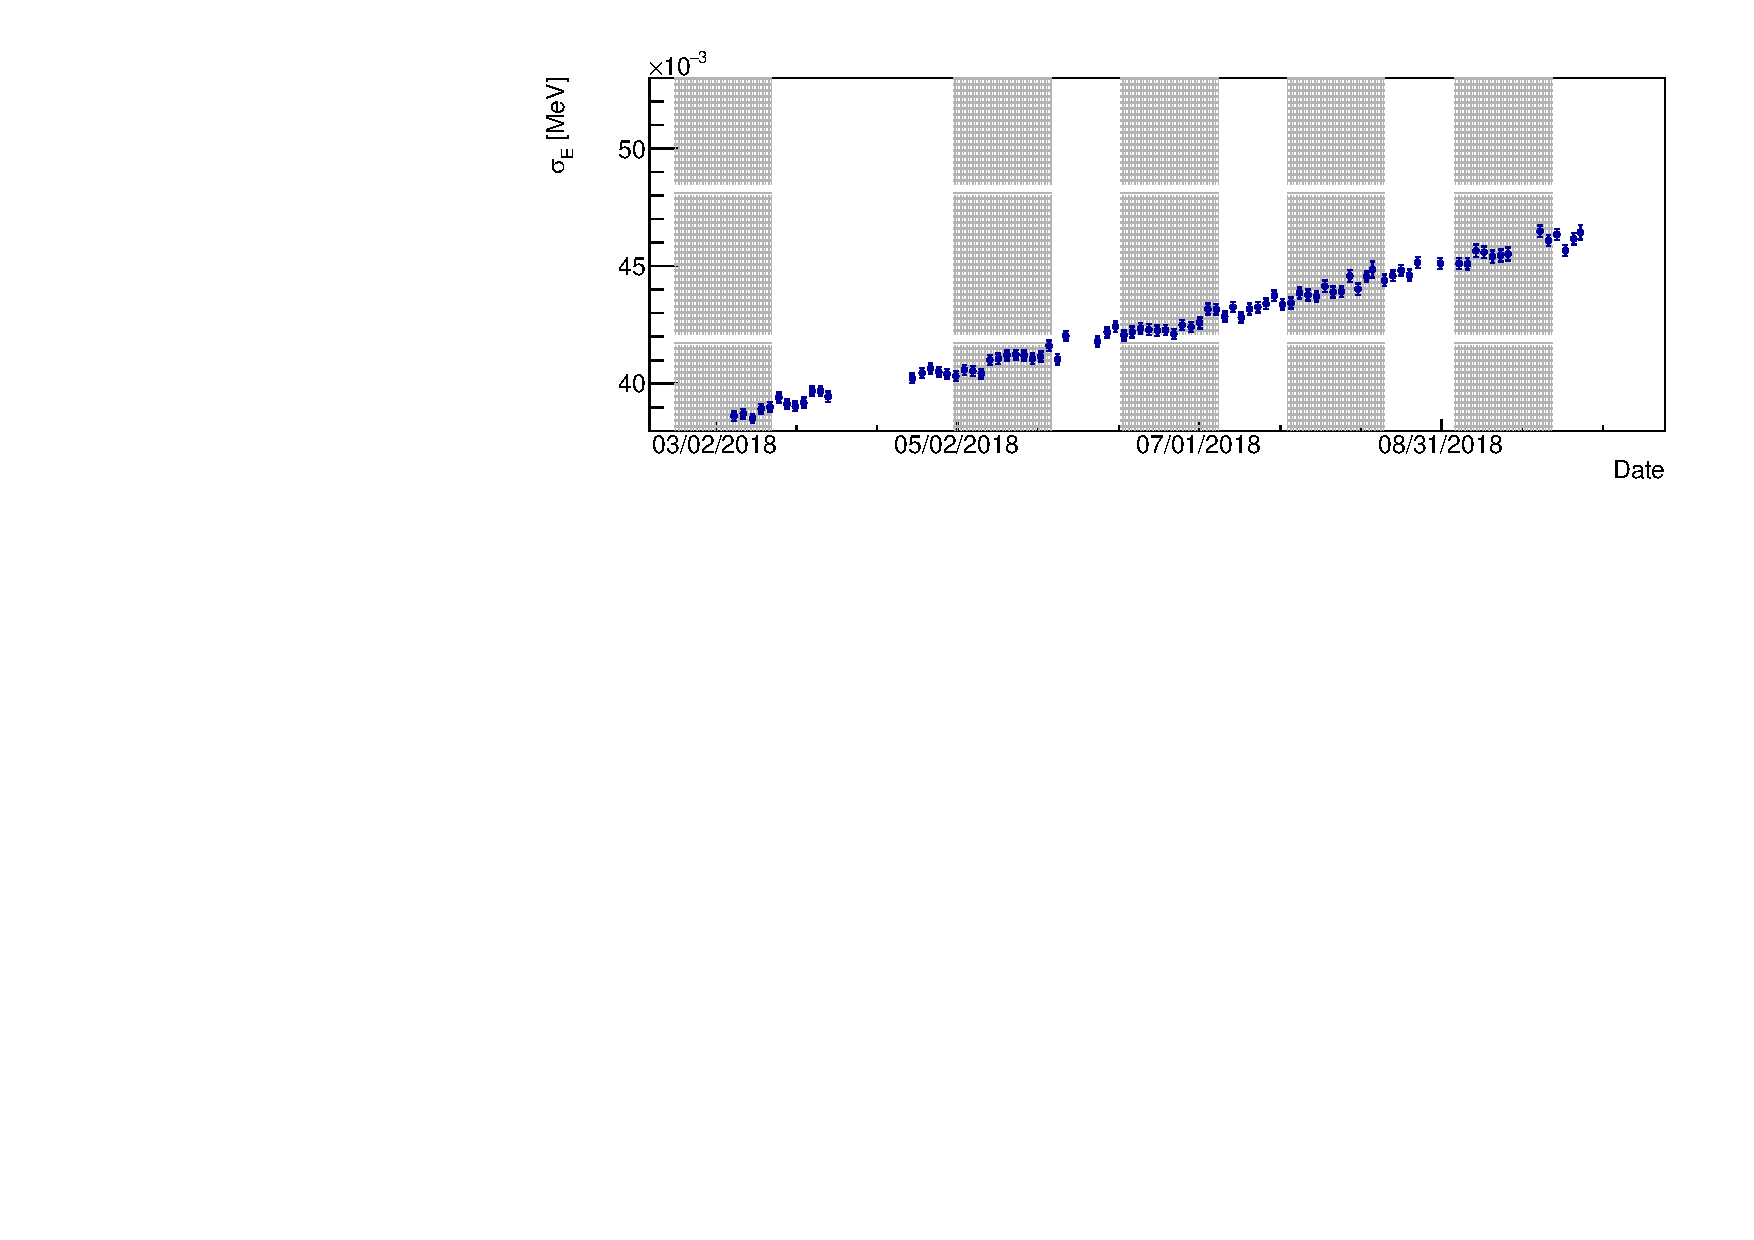
\includegraphics[width=0.9\linewidth]{tex/6-ac227-images/DetPerformance/PoEnSigmaVsTime}
	\caption{}
	\label{fig:poensigmavstime}
\end{subfigure}
\caption{Mean (a) and 1$\sigma$ width (b) of the \Po energy distribution versus time integrated over all segments. Both before applied a correction (E) and after correction (E$_{smear}$) are shown. Shaded areas are reactor on periods.}
\label{fig:EvsT}
\end{figure}

The mean and width of the \Po PSD distribution versus time are shown in Figure~\ref{fig:PSDvsT}.
Similar behavior as was seen in the energy distribution also occurs to the PSD.
Over the 7 month period the PSD distribution increases in width by $\sim$11\% as the mean decreases by $\sim$9\%.
This is accounted for the \Ac analysis by the use of $\sigma$-based cuts on the PSD distributions.

\begin{figure}[h]
\begin{subfigure}{1\linewidth}
	\centering
	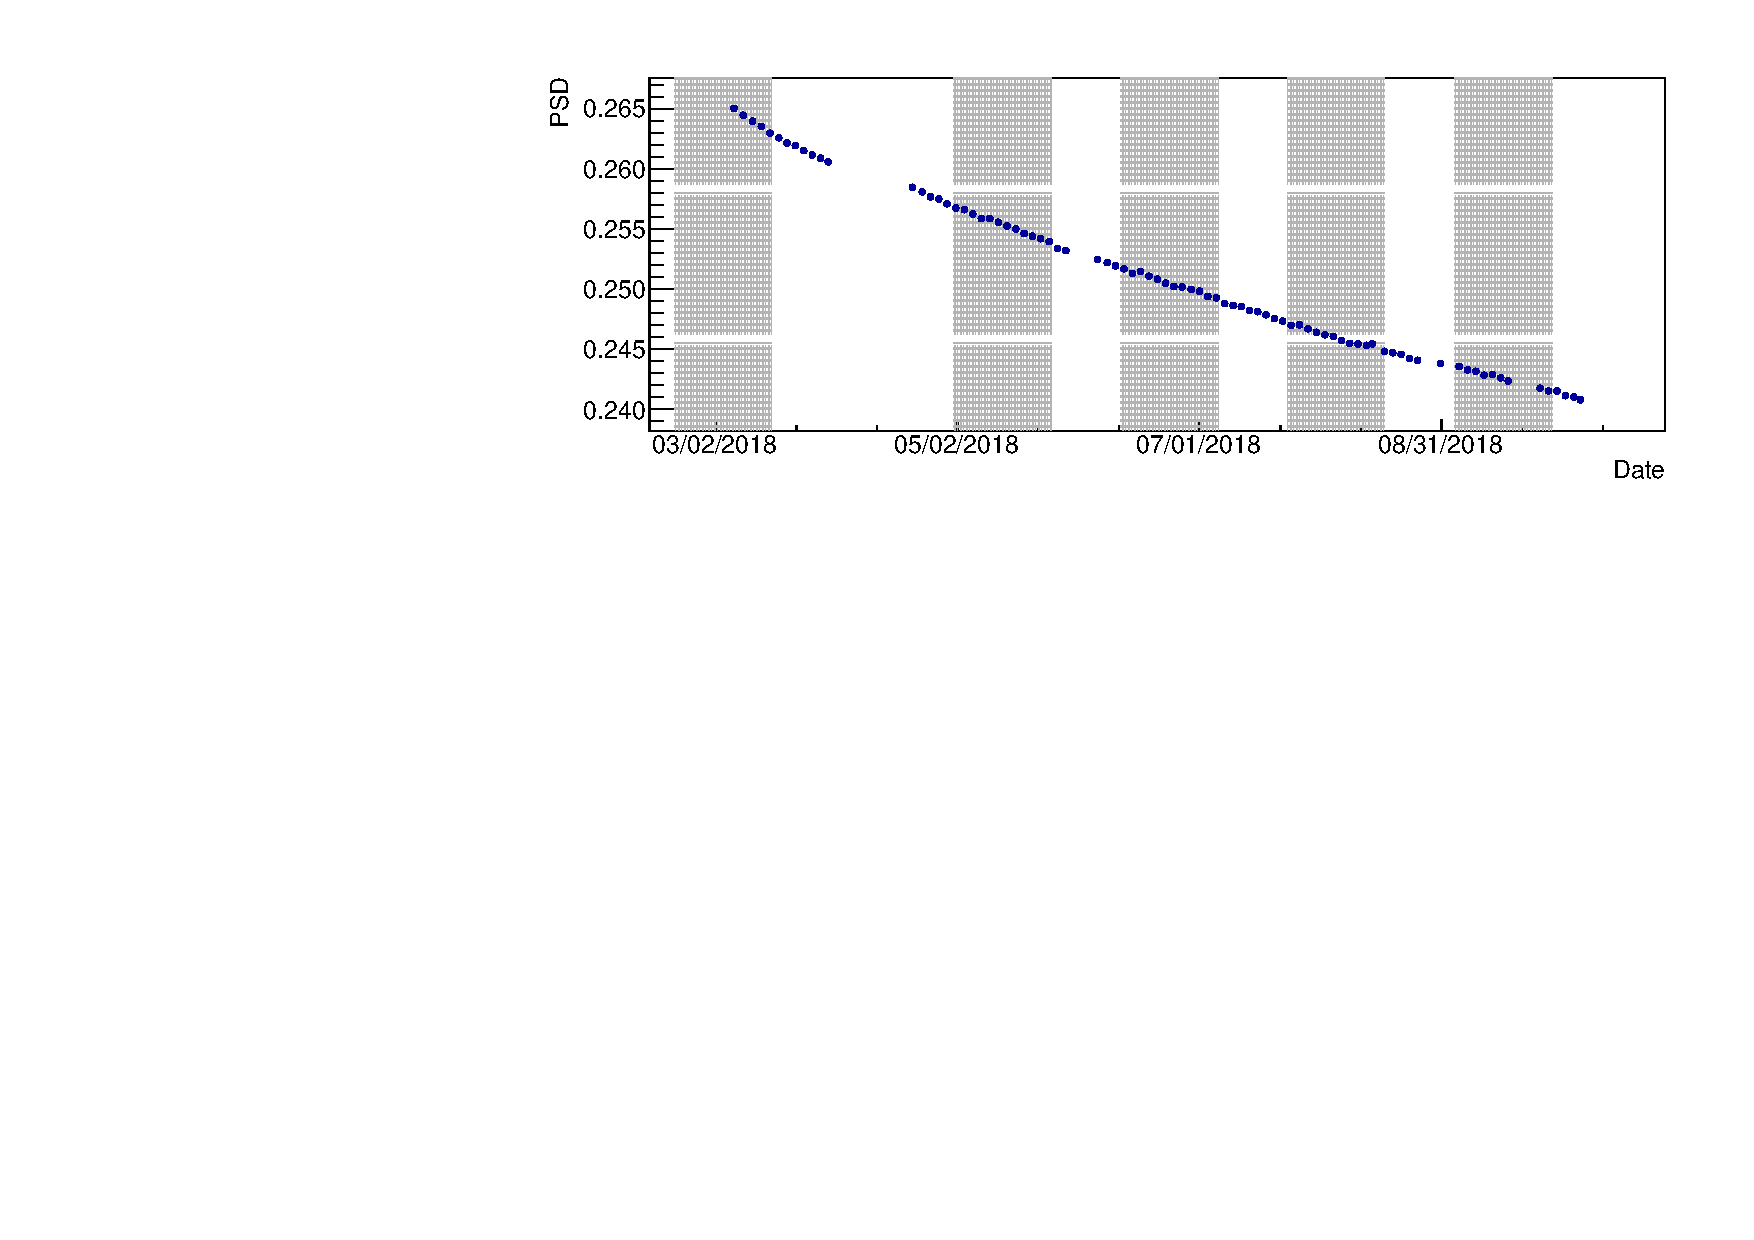
\includegraphics[width=0.9\linewidth]{tex/6-ac227-images/DetPerformance/PoPSDMeanVsTime}
	\caption{}
	\label{fig:popsdmeanvstime}
\end{subfigure}
\begin{subfigure}{1\linewidth}
	\centering
	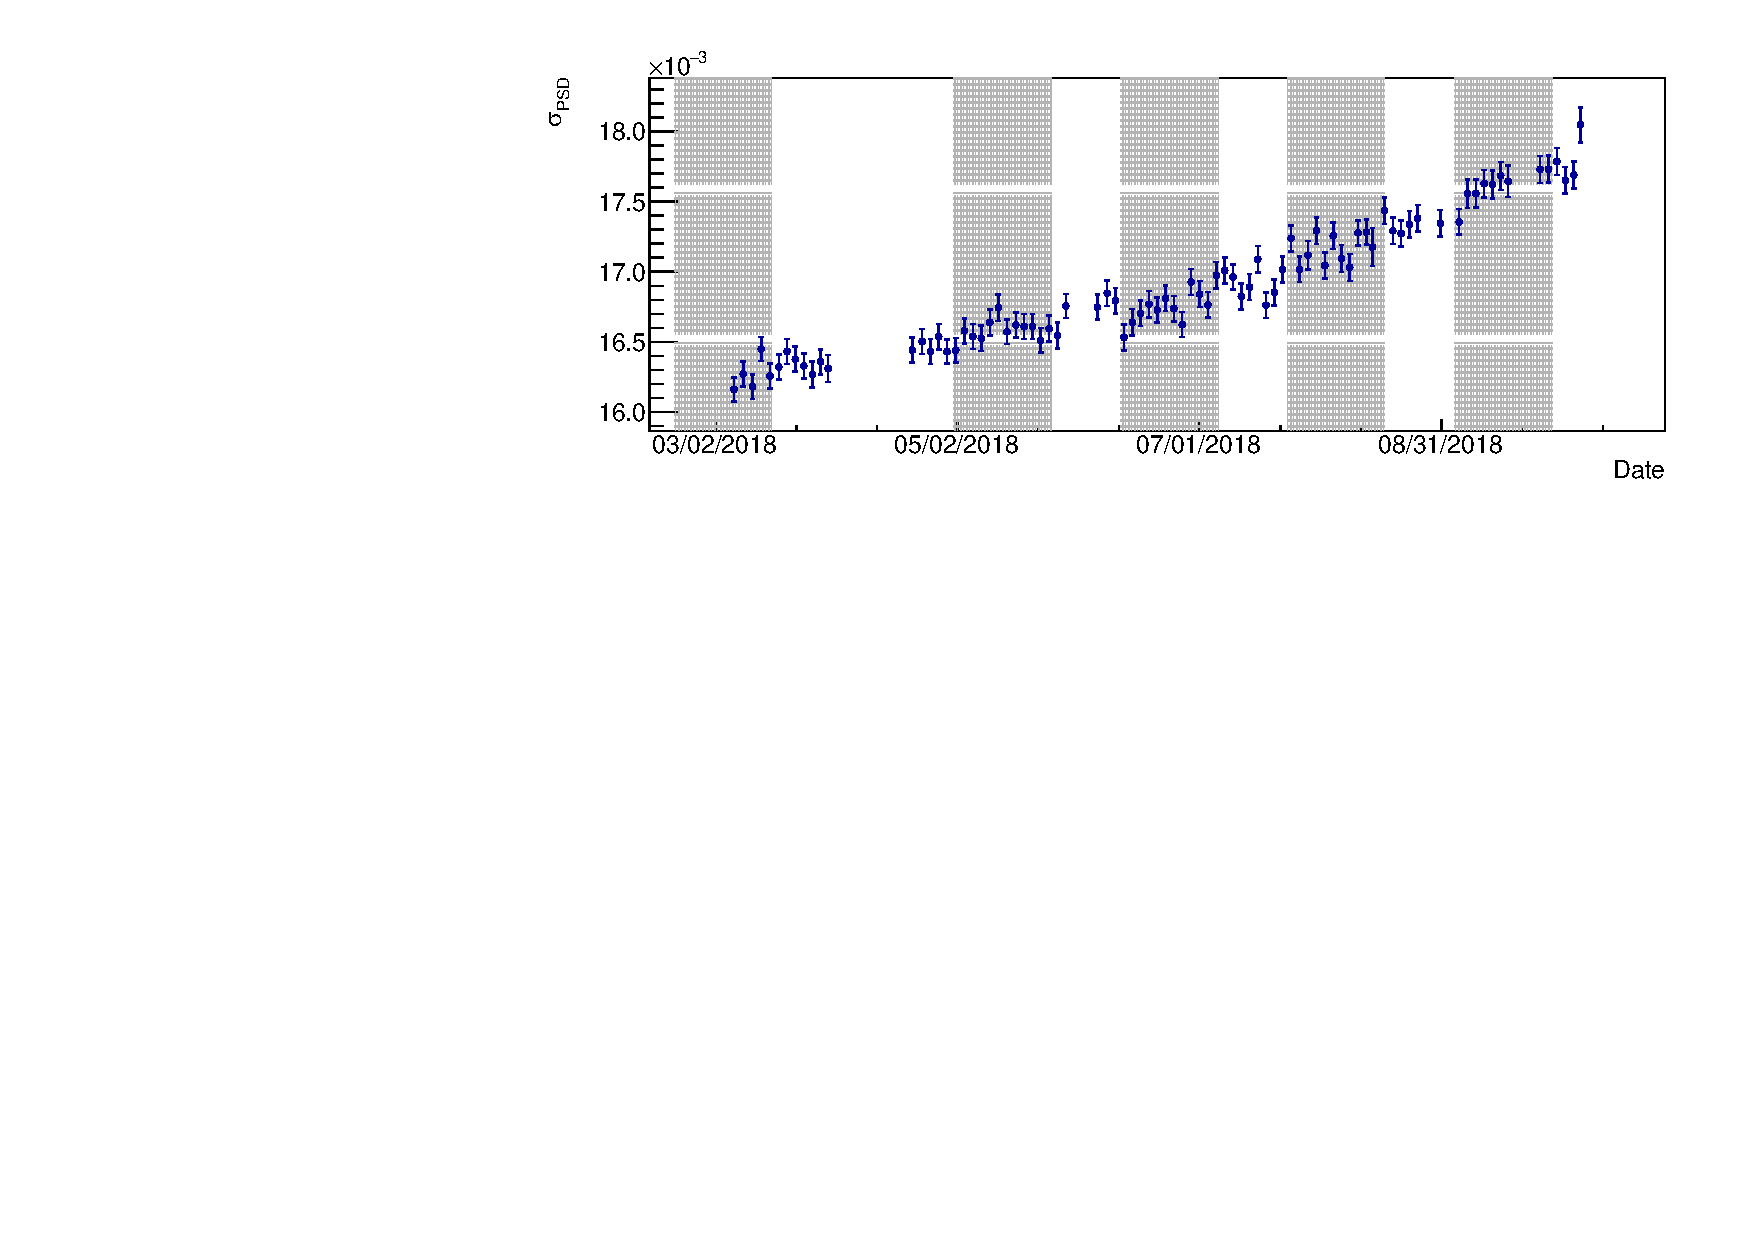
\includegraphics[width=0.9\linewidth]{tex/6-ac227-images/DetPerformance/PoPSDSigmaVsTime}
	\caption{}
	\label{fig:popsdsigmavstime}
\end{subfigure}
\caption{Mean (a) and 1$\sigma$ width (b) of the \Po PSD distribution versus time integrated over all segments. Shaded areas are reactor on periods.}
\label{fig:PSDvsT}
\end{figure}

Position resolution can be determined using the reconstructed position difference of the highly localized coincident alphas.
This is plotted versus time, integrated over all segments, in Figure~\ref{fig:rnpodzsigmavstime}.
It can be seen that the width increases by 7\% over the 7 month period, about 3.5 mm. 
This variation is accounted for in the \Ac analysis in the same way as was done for energy and PSD, by using $\sigma$-based cuts.

\begin{figure}[h]
	\centering
	\includegraphics[width=0.9\linewidth]{tex/6-ac227-images/DetPerformance/RnPoDzSigmaVsTime}
	\caption{1$\sigma$ width of the $\Delta z$ distribution versus time. Shaded areas are reactor on periods.}
	\label{fig:rnpodzsigmavstime}
\end{figure}

Features of the \Po distribution are also useful to compare variations between segments. 
Figure~\ref{fig:histsvsseg} shows the distributions of the \Po energy, energy resolution, position, and position resolution in all individual segments. 
For Hamamatsu segments the energy scale and resolution are identical between segments to within $\sim \pm$0.25\% and $\sim \pm$6.5\% respectively. 
The ET segments vary more than the Hamamatsu segments, but for the case of the IBD analysis these segments are considered outside the fiducial volume.

The position of events along the length of a segment, $z$, was reconstructed individually for each cell by a combination of differences in timing and light yield between the two PMTs. 
As a result, the reconstructed $z$-position may vary from cell to cell. 
The relative alignment of the reconstructed $z$-position between segments can be observed by looking at the distribution of the mean of the position distribution for all segments.
It can be seen that, for Hamamatsu segments, all position reconstructions were aligned within $\pm$7 mm. 
The width of the $\Delta z$ distributions in Hamamatsu segments have a segment-to-segment variation of $\sim \pm$4 mm.

\Ac has proven to be useful in tracking energy, energy resolution, position, and position resolution over time and between segments.
Though IBD events are characteristically very different from RnPo $\alpha$ events, in energy and spatial event topologies, these distributions help to provide limits on systematic errors applied to the IBD analysis due to changing resolution effects and position reconstruction.
They also provide useful cross-checks for the behavior of new variables, such as $E_{smear}$, and tracking calibration performance over time.

\begin{figure}[H]
	\centering
	\includegraphics[width=1\linewidth]{tex/6-ac227-images/DetPerformance/HistsVsSeg}
	\caption{Segment-to-segment stability of the \Po energy (a), energy resolution (b), position reconstruction (c), and position resolution (d). Distributions are shown separately for Hamamatsu and ET segments.}
	\label{fig:histsvsseg}
\end{figure}

\subsection{\Ac Rate versus Time}

Observing the rate of \Ac in the AD over time provides a cross-check of the analysis while giving insight into the behavior of the detector.
Figure~\ref{fig:ratevstimefit} shows the \Ac rate measured versus time, integrated over all segments.
This was fit twice with an exponential of the form
\begin{equation}
	f(t) = R_0e^{\frac{-(t-t_0)\ln(2)}{t_{1/2}}},
	\label{eq:DtExp}
\end{equation}
where $R_0$ is allowed to vary both times and $t_{1/2}$, the half-life of \Ac (21.772~$\pm$~0.003~yrs), is fixed for one fit and allowed to vary in the other.
	
\begin{figure}[!b]
	\centering
	\includegraphics[width=1\linewidth]{tex/6-ac227-images/RateVsTime/RateVsTime_Fit}
	\caption{\Ac rate as measured versus time integrated over all segments. Fit with two exponentials, one in which the half-life of \Ac is allowed to vary (red) and one in which it is fixed (black). Errors are statistical. Shaded areas are reactor on periods.}
	\label{fig:ratevstimefit}
\end{figure}

When the half-life is allowed to vary, the fit returns a half-life of 11.73~$\pm$~0.69~yrs, suggesting that the measured rate of \Ac in the AD is falling 1.56 $\pm$ 0.21 \% faster than expectation over a period of 7 months.
The reason for this discrepancy is unclear.
Measurements of the \Po lifetime versus time, Figure~\ref{fig:lifetimevstime}, are consistent with its accepted lifetime, suggesting that the analysis is correctly accepting and measuring RnPo events.
The use of $\sigma$-based cuts for energy, PSD, and $\Delta z$ result in efficiencies that are always 99.9\% or higher, ruling out loss of events due to changing resolution as a solution.

One hypothesis is that \Ac is falling out of the LiLS solution. 
The process by which this would occur is unclear, but, in an attempt to gain more insight the detector was split into five sections of two rows each, as shown in Figure~\ref{fig:adsegmentsrows}.
The \Ac rate in each of these sections was measured and fit with the exponential in Equation~\ref{eq:DtExp}, allowing the half-life to vary.
See Figure~\ref{fig:ratevstimerows} for the rates and fits, and Figure~\ref{fig:achalflifevsrow} for the half-lives from the fit results versus row.

Though these results are statistics limited, a gradient from top to bottom can be seen in which the half-life gets shorter as one moves to the top of the detector.
This could be a sign of \Ac falling out of solution and sinking to the bottom of the detector.
The process by which this would happen, though, is unclear.
It is also not understood if it would sink in each individual segment, in which case a gradient might not be measured, or if it would gradually settle to the bottom of the detector volume.

In any case, the fact that the measured \Ac rate deviates from expectation indicates that it is not a perfect proxy for a relative segment-to-segment volume measurement.
To account for this a 1\% systematic error was applied to the segment-by-segment measured \Ac rates.

\begin{figure}[h]
	\centering
	\includegraphics[width=0.5\linewidth]{tex/6-ac227-images/RateVsTime/AD_Segments_Rows}
	\caption{The PROSPECT detector divided into five sections of two rows each. Segments shaded in red are excluded from this analysis.}
	\label{fig:adsegmentsrows}
\end{figure}

\begin{figure}[H]
	\centering
	\includegraphics[width=0.87\linewidth]{tex/6-ac227-images/RateVsTime/RateVsTime_Rows_edit}
	\caption{The measured \Ac rate versus time for each section of two rows, fit with an exponential in which the half-life is allowed to vary.}
	\label{fig:ratevstimerows}
\end{figure}

\begin{figure}[H]
	\centering
	\includegraphics[width=0.8\linewidth]{tex/6-ac227-images/RateVsTime/AcHalfLifevsRow}
	\caption{The half-life results from fitting the \Ac rate versus time for five sections of two rows as shown in Figure~\ref{fig:ratevstimerows}.}
	\label{fig:achalflifevsrow}
\end{figure}



\subsection{\Ac Rate in Individual Segments}

The measured \Ac rate in each segment can be seen in Figure~\ref{fig:ratepercell}. 
Statistical errors for each segment are around 0.6\%.
The average rate, including Hamamatsu and ET segments, is 3.262 $\pm$ 0.002 mHz, in line with the expected factor of 3 less than the desired 0.01 Bq/cell.
The majority of segments vary $\pm$1\% from the average. 

The most glaring outliers are the top row, which are $\sim$1.5\% below average. 
A possible explanation for this is that the top row is not completely filled with scintillator, but the reason for these lower rates is unclear.

If the focus is shifted to only Hamamatsu segments, the fiducial segments, the average is found to be 3.270 $\pm$ 0.002 mHz.
The measured \Ac rates in all fiducial segments agree to within $\pm$2\%.
A histogram of the individual segment rates is shown in Figure~\ref{fig:histratepercell}.
The standard deviation of only the Hamamatsu segments is 0.026~mHz.

\begin{figure}[h]
	\centering
	\includegraphics[width=1\linewidth]{tex/6-ac227-images/RatePerSeg/RatePerCell}
	\caption{The \Ac per individual segment integrated over all time. Dashed line represents the average over all segments. Dotted lines are $\pm$1\% and $\pm$2\% from the average. Blue: Hamamatsu segments, red: ET segments. Errors are statistical.}
	\label{fig:ratepercell}
\end{figure}

\begin{figure}[H]
	\centering
	\includegraphics[width=0.7\linewidth]{tex/6-ac227-images/RatePerSeg/HistRatePerCell}
	\caption{Histogram of the individual segment \Ac rates. Blue (solid): Hamamatsu and ET segments, StdDev = 0.031 mHz. Black (dashed): only Hamamatsu segments, StdDev = 0.026 mHz.}
	\label{fig:histratepercell}
\end{figure}



\subsection{Systematic Errors}

Systematic uncertainties in this analysis come from three sources:
(i) the \Ac rate is falling faster than expectation (for this a 1\% systematic is applied), (ii) the energy, PSD, and $\Delta z$ cut efficiencies are calculated by assuming that all distributions are true Gaussians (for this a 0.15\% error is assigned), and (iii) the presence of other coincident alpha decays in the background that could contaminate the RnPo selection (for this a 0.22\% error is assigned).
It should be noted that up to this point only statistical errors have been presented. 
The systematic errors are never directly applied to the \Ac rates until Section~\ref{sec:AcBaseRates}, in which they are used to visualize how much relative rates as a function of distance from the reactor can vary.  

\subsubsection{Energy, PSD, and $\Delta$z Cuts}
In an effort to determine what level of systematic error to apply to the measured \Ac rates per segment a study was performed on the energy, PSD, and $\Delta z$ cuts.
For each cut (prompt and delay energy and PSD, and $\Delta$z) the width of the cut was changed from 2.5$\sigma$ about the mean to 4.0$\sigma$ in steps of 0.5$\sigma$ with the exception of an added step at 3.8$\sigma$.
The rate per segment was calculated for each of these instances and compared to the rate per segment when all cuts were at 4.0$\sigma$.
An example of the calculated rate per segment when the delayed energy cut is changed in this way can be seen in Figure~\ref{fig:ratevscelldelayecut}. 

For each segment and each cut, the quantity 
\begin{equation}
\frac{R_{4\sigma} - R_{i\sigma}}{R_{4\sigma}}
\label{eq:Sys}
\end{equation}
is calculated, where $R_{4\sigma}$ is the rate when a 4$\sigma$ cut is used and $R_{i\sigma}$ is the rate when a i$\sigma$ cut is used where (i: 2.5, 3.0, 3.5, 3.8).
This process was completed for the total data set and for a simulation set.
The simulation was done as an \Ac source dissolved in the scintillator in the AD with no reactor or ambient background.
The distributions of these results for data can be seen in Figure~\ref{fig:CutSys}.

\begin{figure}[!b]
	\centering
	\includegraphics[width=1\linewidth]{tex/6-ac227-images/Systematics_Cuts/RateVsCell_DelayECut}
	\caption{\Ac rate per segment for different $\sigma$-based cuts on the delayed energy.}
	\label{fig:ratevscelldelayecut}
\end{figure}

The mean of each of these distributions is found and plotted according to the $\sigma$ cut used in Figure~\ref{fig:cutstudyresults}. 
The simulation results are shown in the same figure.
It can be seen that the mean of all distributions converge to zero at 4$\sigma$ with the maximum change in rate being $\sim$0.6 \% at 2.5$\sigma$.

If the method used to calculate efficiency was perfect (implying that all distributions are true Gaussians), then the rate would not depend on the $\sigma$ cut that is applied.
The results of this study show that this is not true and, therefore, a systematic error of 0.15\% will be applied to all measured \Ac rates per segment.

\begin{figure}[H]
	\begin{subfigure}{0.5\linewidth}
		\centering
		\includegraphics[width=0.85\linewidth]{tex/6-ac227-images/Systematics_Cuts/ResidVsCell_PromptECut}
		\caption{Prompt Energy}
	\end{subfigure}
	\begin{subfigure}{0.5\linewidth}
		\centering
		\includegraphics[width=0.85\linewidth]{tex/6-ac227-images/Systematics_Cuts/ResidVsCell_DelayECut}
		\caption{Delay Energy}
	\end{subfigure}
	\begin{subfigure}{0.5\linewidth}
		\centering
		\includegraphics[width=0.85\linewidth]{tex/6-ac227-images/Systematics_Cuts/ResidVsCell_PromptPSDCut}
		\caption{Prompt PSD}
	\end{subfigure}
	\begin{subfigure}{0.5\linewidth}
		\centering
		\includegraphics[width=0.85\linewidth]{tex/6-ac227-images/Systematics_Cuts/ResidVsCell_DelayPSDCut}
		\caption{Delay PSD}
	\end{subfigure}
	\begin{subfigure}{1\linewidth}
		\centering
		\includegraphics[width=0.425\linewidth]{tex/6-ac227-images/Systematics_Cuts/ResidVsCell_DzCut}
		\caption{$\Delta$z}
	\end{subfigure}
	\caption{Pictured here are distributions created by calculating for each cell the difference between the rate using a given $\sigma$ cut and the rate using a 4$\sigma$ cut normalized by the rate using a 4$\sigma$ cut for data.}
	\label{fig:CutSys}
\end{figure}

\begin{figure}[H]
	\centering
	\includegraphics[width=0.8\linewidth]{tex/6-ac227-images/Systematics_Cuts/CutStudyResults}
	\caption{The mean of the distributions shown in Figure~\ref{fig:CutSys}. Solid lines: data. Dashed lines: simulation. Connecting lines are not fits; only meant to help guide the eye of the reader.}
	\label{fig:cutstudyresults}
\end{figure}

\subsubsection{Other Coincident Alphas}

There are two known event types with coincident alphas that occur in the PROSPECT AD that could contaminate the RnPo selection group. The first is an $\alpha$-$\alpha$ coincidence in the naturally occurring $^{232}$Th chain (the chain responsible for $^{212}$Bi$\rightarrow^{212}$Po (BiPo) events): $^{220}$Rn$\rightarrow ^{216}$Po$\rightarrow ^{212}$Pb. 
As listed in Table~\ref{tab:CoincAlpha}, the energy of these alphas fall in the selection range of the \Ac RnPo's (0.48/0.61-1.18 MeV), making it possible for them to be incorrectly identified as \Ac RnPo events.
The $^{232}$Th alphas, though, are not expected to be uniform throughout the detector, creating a possibility of them not being completely removed with the background subtraction.

The other possible event is the triple alpha decay in the \Ac chain: \\ \noindent $^{223}$Ra$\rightarrow$\Rn$\rightarrow$\Po$\rightarrow ^{211}$Pb. 
Choosing an accidental background subtraction window that occurs before a given selected delay event (Po), in the time direction of the $^{223}$Ra contamination, helps to get rid of most of this contamination, but the rate of remaining events can be calculated.

Using the information found in Table~\ref{tab:CoincAlpha} and the time windows chosen for the \Ac RnPo selection it is possible to calculate the amount of contamination that is expected from these other alpha coincidences. 
Starting with the $^{232}$Th RnPo's, the fraction of $^{220}$Rn$\rightarrow ^{216}$Po alphas that are selected as `true' \Ac events, based on energy and time cuts, is $\sim$0.0061. 
If the rate of these events is approximated to be 0.085 Hz (based on a BiPo rate of 0.0547 Hz  \cite{Jones2800:2019}) then the rate of selection is $\sim$0.00052 Hz. 
If we approximate a total \Ac rate of 0.29 Hz, and therefore a rate of 0.24 Hz in the 0.5 - 12.845 ms time window used for selection, then the $^{232}$Th RnPo's will make up $\sim$0.22\% of the \Ac RnPo signal selection in the selection time window.
Therefore, a systematic error of 0.22\% will be applied.

The triple alpha in the \Ac chain contributes much less to the RnPo signal selection. Due to the nature of the background subtraction the probability that $^{223}$Ra$\rightarrow$\Rn coincident events pass both the energy cuts and the subtraction is 0.00083\%. No systematic error will be applied for these event types.

See Table~\ref{tab:CoincAlphaRate} for a summary of the energy and time cut efficiencies for both coincident alpha event types. 

\begin{table}[t]
	\centering
	\begin{tabular}{|c|c|c|c|c|}
		\hline 
		\textbf{Isotope} & \textbf{t$_{1/2}$ [ms]} & \textbf{E [MeV]} & \textbf{QE [MeVee]} & \textbf{1$\sigma$ width [MeVee] (5\% res.)} \\ 
		\hline 
		$^{220}$Rn & 55600 & 6.2881 & 0.5942 & 0.0412 \\ 
		\hline 
		$^{216}$Po & 145 & 6.7783 & 0.6776 & 0.0412 \\ 
		\hline \hline
		$^{223}$Ra & 9.88$\times$10$^{8}$ & 5.7162 & 0.5031 & 0.0355 \\ 
		\hline 
		$^{219}$Rn & 3860 & 6.8191 & 0.6847 & 0.0414 \\ 
		\hline 
		$^{215}$Po & 1.781 & 7.3861 & 0.7876 & 0.0444 \\ 
		\hline 
	\end{tabular} 
	\caption{Dominant $\alpha$ energies for coincident $\alpha$ event chains that could contaminate the \Ac RnPo signal. Also given are the quenched energies (QE) and 1$\sigma$ widths based on a 5\% energy resolution.}
	\label{tab:CoincAlpha}
\end{table}

\begin{table}[H]
	\centering
	\begin{tabular}{|c|c|c|c|c|c|}
		\hline 
		\textbf{Prompt} & \textbf{Delay} & \textbf{t$_{1/2}$ [ms]} & \textbf{Energy Cut Eff.} & \textbf{Time Cut Eff.} & \textbf{Rate [mHz]} \\ 
		\hline 
		$^{220}$Rn & $^{216}$Po & 145 & 0.925 & 0.0066 & 0.52  \\ 
		\hline 
		$^{223}$Ra & $^{219}$Rn & 3860 & 0.815 & 0.000010  & 0.0021 \\ 
		\hline 
	\end{tabular} 
	\caption{Energy and time cut efficiencies and resulting rates (assuming an \Ac rate of 240 mHz) for both coincident $\alpha$ event chains that could contribute to contamination of the \Ac RnPo signal selection.}
	\label{tab:CoincAlphaRate}
\end{table}


\subsection{\Ac Rates per Baseline} \label{sec:AcBaseRates}

The original goal of adding \Ac to the PROSPECT detector was to measure relative volume differences and apply these corrections to the oscillation analysis. 
The oscillation analysis is carried out by dividing the detector into baselines, or distances from the reactor core, and comparing the measured spectra between baselines.
A similar process can be done for the \Ac rates, and then corrections can be applied to the number of IBD counts versus baseline based on the \Ac results.

The detector was divided into 10 individual baselines, where baseline 1 is closest to the reactor core.
Figure~\ref{fig:adsegments} shows the configuration of baselines that was chosen for this data set.
The \Ac rate measured for each segment was then averaged over each baseline (error-weighted) and then plotted relative to the average rate in the first baseline.
The results of this can be seen in Figure~\ref{fig:ratevsbaseline}.

It can be seen that the average rates vary less than 0.5\% over all baselines.
The statistics of this data set do not require volume corrections at this level, but these results provide a lower limit that could be applied to the oscillation analysis.\footnote{As the oscillation analysis for this data set is not yet completed, these results cannot currently be applied as corrections to the IBD rate versus baseline. 
Instead, the same analysis described in this chapter was applied to the data set used for the published oscillation results and corrections were applied accordingly, as described in the next chapter.}
For a data set with large statistics, in which volume variations could become an important systematic error, this method of adding \Ac and measuring the decay rates as a proxy for volume is proven to be effective.

\begin{figure}[!t]
	\centering
	\includegraphics[width=0.6\linewidth]{tex/6-ac227-images/Baseline/AD_Segments}
	\caption{The PROSPECT AD divided into 10 baselines, where baseline 1 is closest to the reactor. Segments in white are either fiducial segments or were turned off.}
	\label{fig:adsegments}
\end{figure}

\begin{figure}[h]
	\centering
	\includegraphics[width=0.9\linewidth]{tex/6-ac227-images/Baseline/RateVsBaseline_PRD_Relative}
	\caption{The \Ac rate averaged over each of the 10 defined baselines and relative to the first baseline. Error bars are statistical, systematic errors are shown as the shaded region.}
	\label{fig:ratevsbaseline}
\end{figure}






\chapter{\uppercase{Inverse Beta Decay Event Selection}}

\section{Selection Criteria and Efficiency}

\section{Properties of the Event Selection}


\chapter{\uppercase{Neutrino Oscillation in the PROSPECT AD}}

\section{Analysis Method}

\section{Result}


\chapter{CONCLUSIONS}

.


%: ----------------------------------------------------------------------
%: Back matter: appendicies, references, etc.
%: ----------------------------------------------------------------------

% the back matter: appendix and references close the thesis

%: ----------------------------------------------------------------------
%: Bibliography
%: ----------------------------------------------------------------------

\bibliographystyle{apsrev}
\renewcommand{\bibname}{REFERENCES} % changes the header; default: Bibliography

%\bibliographystyle{unsrt}   % unsorted references: appear in order they're cited

\bibliography{ThesisBib}

% Appendix
% NOTE: We add special commands in the ./Appendix/*.tex files
% to make sure that only chapter-level information shows up in the TOC.
%\renewcommand\chaptername{APPENDIX}
%\renewcommand{\appendixname}{APPENDIX}
%\include{Appendix/appendix}

\printindex
\end{document}
